%********************************************%
%*       Generated from PreTeXt source      *%
%*       on 2025-09-09T09:53:32-04:00       *%
%*   A recent stable commit (2022-07-01):   *%
%* 6c761d3dba23af92cba35001c852aac04ae99a5f *%
%*                                          *%
%*         https://pretextbook.org          *%
%*                                          *%
%********************************************%
\documentclass[oneside,10pt,]{book}
%% Custom Preamble Entries, early (use latex.preamble.early)
%% Default LaTeX packages
%%   1.  always employed (or nearly so) for some purpose, or
%%   2.  a stylewriter may assume their presence
\usepackage[total={6.5in,9in}]{geometry}
%% Some aspects of the preamble are conditional,
%% the LaTeX engine is one such determinant
\usepackage{ifthen}
%% etoolbox has a variety of modern conveniences
\usepackage{etoolbox}
\usepackage{ifxetex,ifluatex}
%% Raster graphics inclusion
\usepackage{graphicx}
%% Color support, xcolor package
%% Always loaded, for: add/delete text, author tools
%% Here, since tcolorbox loads tikz, and tikz loads xcolor
\PassOptionsToPackage{dvipsnames,svgnames,table}{xcolor}
\usepackage{xcolor}
%% begin: defined colors, via xcolor package, for styling
%% end: defined colors, via xcolor package, for styling
%% Colored boxes, and much more, though mostly styling
%% skins library provides "enhanced" skin, employing tikzpicture
%% boxes may be configured as "breakable" or "unbreakable"
%% "raster" controls grids of boxes, aka side-by-side
\usepackage{tcolorbox}
\tcbuselibrary{skins}
\tcbuselibrary{breakable}
\tcbuselibrary{raster}
%% We load some "stock" tcolorbox styles that we use a lot
%% Placement here is provisional, there will be some color work also
%% First, black on white, no border, transparent, but no assumption about titles
\tcbset{ bwminimalstyle/.style={size=minimal, boxrule=-0.3pt, frame empty,
colback=white, colbacktitle=white, coltitle=black, opacityfill=0.0} }
%% Second, bold title, run-in to text/paragraph/heading
%% Space afterwards will be controlled by environment,
%% independent of constructions of the tcb title
%% Places \blocktitlefont onto many block titles
\tcbset{ runintitlestyle/.style={fonttitle=\blocktitlefont\upshape\bfseries, attach title to upper} }
%% Spacing prior to each exercise, anywhere
\tcbset{ exercisespacingstyle/.style={before skip={1.5ex plus 0.5ex}} }
%% Spacing prior to each block
\tcbset{ blockspacingstyle/.style={before skip={2.0ex plus 0.5ex}} }
%% xparse allows the construction of more robust commands,
%% this is a necessity for isolating styling and behavior
%% The tcolorbox library of the same name loads the base library
\tcbuselibrary{xparse}
%% The tcolorbox library loads TikZ, its calc package is generally useful,
%% and is necessary for some smaller documents that use partial tcolor boxes
%% See:  https://github.com/PreTeXtBook/pretext/issues/1624
\usetikzlibrary{calc}
%% We use some more exotic tcolorbox keys to restore indentation to parboxes
\tcbuselibrary{hooks}
%% Save default paragraph indentation and parskip for use later, when adjusting parboxes
\newlength{\normalparindent}
\newlength{\normalparskip}
\AtBeginDocument{\setlength{\normalparindent}{\parindent}}
\AtBeginDocument{\setlength{\normalparskip}{\parskip}}
\newcommand{\setparstyle}{\setlength{\parindent}{\normalparindent}\setlength{\parskip}{\normalparskip}}%% Hyperref should be here, but likes to be loaded late
%%
%% Inline math delimiters, \(, \), need to be robust
%% 2016-01-31:  latexrelease.sty  supersedes  fixltx2e.sty
%% If  latexrelease.sty  exists, bugfix is in kernel
%% If not, bugfix is in  fixltx2e.sty
%% See:  https://tug.org/TUGboat/tb36-3/tb114ltnews22.pdf
%% and read "Fewer fragile commands" in distribution's  latexchanges.pdf
\IfFileExists{latexrelease.sty}{}{\usepackage{fixltx2e}}
%% Footnote counters and part/chapter counters are manipulated
%% April 2018:  chngcntr  commands now integrated into the kernel,
%% but circa 2018/2019 the package would still try to redefine them,
%% so we need to do the work of loading conditionally for old kernels.
%% From version 1.1a,  chngcntr  should detect defintions made by LaTeX kernel.
\ifdefined\counterwithin
\else
    \usepackage{chngcntr}
\fi
%% Text height identically 9 inches, text width varies on point size
%% See Bringhurst 2.1.1 on measure for recommendations
%% 75 characters per line (count spaces, punctuation) is target
%% which is the upper limit of Bringhurst's recommendations
\geometry{letterpaper,total={340pt,9.0in}}
%% Custom Page Layout Adjustments (use publisher page-geometry entry)
%% This LaTeX file may be compiled with pdflatex, xelatex, or lualatex executables
%% LuaTeX is not explicitly supported, but we do accept additions from knowledgeable users
%% The conditional below provides  pdflatex  specific configuration last
%% begin: engine-specific capabilities
\ifthenelse{\boolean{xetex} \or \boolean{luatex}}{%
%% begin: xelatex and lualatex-specific default configuration
\ifxetex\usepackage{xltxtra}\fi
%% realscripts is the only part of xltxtra relevant to lualatex
\ifluatex\usepackage{realscripts}\fi
%% end:   xelatex and lualatex-specific default configuration
}{
%% begin: pdflatex-specific default configuration
%% We assume a PreTeXt XML source file may have Unicode characters
%% and so we ask LaTeX to parse a UTF-8 encoded file
%% This may work well for accented characters in Western language,
%% but not with Greek, Asian languages, etc.
%% When this is not good enough, switch to the  xelatex  engine
%% where Unicode is better supported (encouraged, even)
\usepackage[utf8]{inputenc}
%% end: pdflatex-specific default configuration
}
%% end:   engine-specific capabilities
%%
%% Fonts.  Conditional on LaTex engine employed.
%% Default Text Font: The Latin Modern fonts are
%% "enhanced versions of the [original TeX] Computer Modern fonts."
%% We use them as the default text font for PreTeXt output.
%% Default Monospace font: Inconsolata (aka zi4)
%% Sponsored by TUG: http://levien.com/type/myfonts/inconsolata.html
%% Loaded for documents with intentional objects requiring monospace
%% See package documentation for excellent instructions
%% fontspec will work universally if we use filename to locate OTF files
%% Loads the "upquote" package as needed, so we don't have to
%% Upright quotes might come from the  textcomp  package, which we also use
%% We employ the shapely \ell to match Google Font version
%% pdflatex: "varl" package option produces shapely \ell
%% pdflatex: "var0" package option produces plain zero (not used)
%% pdflatex: "varqu" package option produces best upright quotes
%% xelatex,lualatex: add OTF StylisticSet 1 for shapely \ell
%% xelatex,lualatex: add OTF StylisticSet 2 for plain zero (not used)
%% xelatex,lualatex: add OTF StylisticSet 3 for upright quotes
%%
%% Automatic Font Control
%% Portions of a document, are, or may, be affected by defined commands
%% These are perhaps more flexible when using  xelatex  rather than  pdflatex
%% The following definitions are meant to be re-defined in a style, using \renewcommand
%% They are scoped when employed (in a TeX group), and so should not be defined with an argument
\newcommand{\divisionfont}{\relax}
\newcommand{\blocktitlefont}{\relax}
\newcommand{\contentsfont}{\relax}
\newcommand{\pagefont}{\relax}
\newcommand{\tabularfont}{\relax}
\newcommand{\xreffont}{\relax}
\newcommand{\titlepagefont}{\relax}
%%
\ifthenelse{\boolean{xetex} \or \boolean{luatex}}{%
%% begin: font setup and configuration for use with xelatex
%% Generally, xelatex is necessary for non-Western fonts
%% fontspec package provides extensive control of system fonts,
%% meaning *.otf (OpenType), and apparently *.ttf (TrueType)
%% that live *outside* your TeX/MF tree, and are controlled by your *system*
%% (it is possible that a TeX distribution will place fonts in a system location)
%%
%% The fontspec package is the best vehicle for using different fonts in  xelatex
%% So we load it always, no matter what a publisher or style might want
%%
\usepackage{fontspec}
%%
%% begin: xelatex main font ("font-xelatex-main" template)
%% Latin Modern Roman is the default font for xelatex and so is loaded with a TU encoding
%% *in the format* so we can't touch it, only perhaps adjust it later
%% in one of two ways (then known by NFSS names such as "lmr")
%% (1) via NFSS with font family names such as "lmr" and "lmss"
%% (2) via fontspec with commands like \setmainfont{Latin Modern Roman}
%% The latter requires the font to be known at the system-level by its font name,
%% but will give access to OTF font features through optional arguments
%% https://tex.stackexchange.com/questions/470008/
%% where-and-how-does-fontspec-sty-specify-the-default-font-latin-modern-roman
%% http://tex.stackexchange.com/questions/115321
%% /how-to-optimize-latin-modern-font-with-xelatex
%%
%% end:   xelatex main font ("font-xelatex-main" template)
%% begin: xelatex mono font ("font-xelatex-mono" template)
%% (conditional on non-trivial uses being present in source)
\IfFontExistsTF{Inconsolatazi4-Regular.otf}{}{\GenericError{}{The font "Inconsolatazi4-Regular.otf" requested by PreTeXt output processed by the  xelatex  executable is not available.  Either a file cannot be located in default locations via a filename, or a font is not known by its name as part of your system.}{Consult the PreTeXt Guide for help with LaTeX fonts, or perhaps try using  pdflatex  as a test.}{}}
\IfFontExistsTF{Inconsolatazi4-Bold.otf}{}{\GenericError{}{The font "Inconsolatazi4-Bold.otf" requested by PreTeXt output processed by the  xelatex  executable is not available.  Either a file cannot be located in default locations via a filename, or a font is not known by its name as part of your system.}{Consult the PreTeXt Guide for help with LaTeX fonts, or perhaps try using  pdflatex  as a test.}{}}
\usepackage{zi4}
\setmonofont[BoldFont=Inconsolatazi4-Bold.otf,StylisticSet={1,3}]{Inconsolatazi4-Regular.otf}
%% end:   xelatex mono font ("font-xelatex-mono" template)
%% begin: xelatex font adjustments ("font-xelatex-style" template)
%% end:   xelatex font adjustments ("font-xelatex-style" template)
%%
%% Extensive support for other languages
\usepackage{polyglossia}
%% Set main/default language based on pretext/@xml:lang value
%% document language code is "en-US", US English
%% usmax variant has extra hypenation
\setmainlanguage[variant=usmax]{english}
%% Enable secondary languages based on discovery of @xml:lang values
%% Enable fonts/scripts based on discovery of @xml:lang values
%% Western languages should be ably covered by Latin Modern Roman
%% end:   font setup and configuration for use with xelatex
}{%
%% begin: font setup and configuration for use with pdflatex
%% begin: pdflatex main font ("font-pdflatex-main" template)
\usepackage{lmodern}
\usepackage[T1]{fontenc}
%% end:   pdflatex main font ("font-pdflatex-main" template)
%% begin: pdflatex mono font ("font-pdflatex-mono" template)
%% (conditional on non-trivial uses being present in source)
\usepackage[varqu,varl]{inconsolata}
%% end:   pdflatex mono font ("font-pdflatex-mono" template)
%% begin: pdflatex font adjustments ("font-pdflatex-style" template)
%% end:   pdflatex font adjustments ("font-pdflatex-style" template)
%% end:   font setup and configuration for use with pdflatex
}
%% Micromanage spacing, etc.  The named "microtype-options"
%% template may be employed to fine-tune package behavior
\usepackage{microtype}
%% Symbols, align environment, commutative diagrams, bracket-matrix
\usepackage{amsmath}
\usepackage{amscd}
\usepackage{amssymb}
%% allow page breaks within display mathematics anywhere
%% level 4 is maximally permissive
%% this is exactly the opposite of AMSmath package philosophy
%% there are per-display, and per-equation options to control this
%% split, aligned, gathered, and alignedat are not affected
\allowdisplaybreaks[4]
%% allow more columns to a matrix
%% can make this even bigger by overriding with  latex.preamble.late  processing option
\setcounter{MaxMatrixCols}{30}
%%
%%
%% Division Titles, and Page Headers/Footers
%% titlesec package, loading "titleps" package cooperatively
%% See code comments about the necessity and purpose of "explicit" option.
%% The "newparttoc" option causes a consistent entry for parts in the ToC
%% file, but it is only effective if there is a \titleformat for \part.
%% "pagestyles" loads the  titleps  package cooperatively.
\usepackage[explicit, newparttoc, pagestyles]{titlesec}
%% The companion titletoc package for the ToC.
\usepackage{titletoc}
%% Fixes a bug with transition from chapters to appendices in a "book"
%% See generating XSL code for more details about necessity
\newtitlemark{\chaptertitlename}
%% begin: customizations of page styles via the modal "titleps-style" template
%% Designed to use commands from the LaTeX "titleps" package
%% Plain pages should have the same font for page numbers
\renewpagestyle{plain}{%
\setfoot{}{\pagefont\thepage}{}%
}%
%% Single pages as in default LaTeX
\renewpagestyle{headings}{%
\sethead{\pagefont\slshape\MakeUppercase{\ifthechapter{\chaptertitlename\space\thechapter.\space}{}\chaptertitle}}{}{\pagefont\thepage}%
}%
\pagestyle{headings}
%% end: customizations of page styles via the modal "titleps-style" template
%%
%% Create globally-available macros to be provided for style writers
%% These are redefined for each occurence of each division
\newcommand{\divisionnameptx}{\relax}%
\newcommand{\titleptx}{\relax}%
\newcommand{\subtitleptx}{\relax}%
\newcommand{\shortitleptx}{\relax}%
\newcommand{\authorsptx}{\relax}%
\newcommand{\epigraphptx}{\relax}%
%% Create environments for possible occurences of each division
%% Environment for a PTX "preface" at the level of a LaTeX "chapter"
\NewDocumentEnvironment{preface}{mmmmmmm}
{%
\renewcommand{\divisionnameptx}{#1}%
\renewcommand{\titleptx}{#2}%
\renewcommand{\subtitleptx}{#3}%
\renewcommand{\shortitleptx}{#4}%
\renewcommand{\authorsptx}{#5}%
\renewcommand{\epigraphptx}{#6}%
\chapter*{#2}%
\addcontentsline{toc}{chapter}{#4}
\label{#7}%
}{}%
%% Environment for a PTX "chapter" at the level of a LaTeX "chapter"
\NewDocumentEnvironment{chapterptx}{mmmmmmm}
{%
\renewcommand{\divisionnameptx}{#1}%
\renewcommand{\titleptx}{#2}%
\renewcommand{\subtitleptx}{#3}%
\renewcommand{\shortitleptx}{#4}%
\renewcommand{\authorsptx}{#5}%
\renewcommand{\epigraphptx}{#6}%
\chapter[{#4}]{#2}%
\label{#7}%
}{}%
%% Environment for a PTX "section" at the level of a LaTeX "section"
\NewDocumentEnvironment{sectionptx}{mmmmmmm}
{%
\renewcommand{\divisionnameptx}{#1}%
\renewcommand{\titleptx}{#2}%
\renewcommand{\subtitleptx}{#3}%
\renewcommand{\shortitleptx}{#4}%
\renewcommand{\authorsptx}{#5}%
\renewcommand{\epigraphptx}{#6}%
\section[{#4}]{#2}%
\label{#7}%
}{}%
%% Environment for a PTX "subsection" at the level of a LaTeX "subsection"
\NewDocumentEnvironment{subsectionptx}{mmmmmmm}
{%
\renewcommand{\divisionnameptx}{#1}%
\renewcommand{\titleptx}{#2}%
\renewcommand{\subtitleptx}{#3}%
\renewcommand{\shortitleptx}{#4}%
\renewcommand{\authorsptx}{#5}%
\renewcommand{\epigraphptx}{#6}%
\subsection[{#4}]{#2}%
\label{#7}%
}{}%
%% Environment for a PTX "subsubsection" at the level of a LaTeX "subsubsection"
\NewDocumentEnvironment{subsubsectionptx}{mmmmmmm}
{%
\renewcommand{\divisionnameptx}{#1}%
\renewcommand{\titleptx}{#2}%
\renewcommand{\subtitleptx}{#3}%
\renewcommand{\shortitleptx}{#4}%
\renewcommand{\authorsptx}{#5}%
\renewcommand{\epigraphptx}{#6}%
\subsubsection[{#4}]{#2}%
\label{#7}%
}{}%
%% Environment for a PTX "appendix" at the level of a LaTeX "chapter"
\NewDocumentEnvironment{appendixptx}{mmmmmmm}
{%
\renewcommand{\divisionnameptx}{#1}%
\renewcommand{\titleptx}{#2}%
\renewcommand{\subtitleptx}{#3}%
\renewcommand{\shortitleptx}{#4}%
\renewcommand{\authorsptx}{#5}%
\renewcommand{\epigraphptx}{#6}%
\chapter[{#4}]{#2}%
\label{#7}%
}{}%
%%
%% Styles for six traditional LaTeX divisions
\titleformat{\part}[display]
{\divisionfont\Huge\bfseries\centering}{\divisionnameptx\space\thepart}{30pt}{\Huge#1}
[{\Large\centering\authorsptx}]
\titleformat{\chapter}[display]
{\divisionfont\huge\bfseries}{\divisionnameptx\space\thechapter}{20pt}{\Huge#1}
[{\Large\authorsptx}]
\titleformat{name=\chapter,numberless}[display]
{\divisionfont\huge\bfseries}{}{0pt}{#1}
[{\Large\authorsptx}]
\titlespacing*{\chapter}{0pt}{50pt}{40pt}
\titleformat{\section}[hang]
{\divisionfont\Large\bfseries}{\thesection}{1ex}{#1}
[{\large\authorsptx}]
\titleformat{name=\section,numberless}[block]
{\divisionfont\Large\bfseries}{}{0pt}{#1}
[{\large\authorsptx}]
\titlespacing*{\section}{0pt}{3.5ex plus 1ex minus .2ex}{2.3ex plus .2ex}
\titleformat{\subsection}[hang]
{\divisionfont\large\bfseries}{\thesubsection}{1ex}{#1}
[{\normalsize\authorsptx}]
\titleformat{name=\subsection,numberless}[block]
{\divisionfont\large\bfseries}{}{0pt}{#1}
[{\normalsize\authorsptx}]
\titlespacing*{\subsection}{0pt}{3.25ex plus 1ex minus .2ex}{1.5ex plus .2ex}
\titleformat{\subsubsection}[hang]
{\divisionfont\normalsize\bfseries}{\thesubsubsection}{1em}{#1}
[{\small\authorsptx}]
\titleformat{name=\subsubsection,numberless}[block]
{\divisionfont\normalsize\bfseries}{}{0pt}{#1}
[{\normalsize\authorsptx}]
\titlespacing*{\subsubsection}{0pt}{3.25ex plus 1ex minus .2ex}{1.5ex plus .2ex}
\titleformat{\paragraph}[hang]
{\divisionfont\normalsize\bfseries}{\theparagraph}{1em}{#1}
[{\small\authorsptx}]
\titleformat{name=\paragraph,numberless}[block]
{\divisionfont\normalsize\bfseries}{}{0pt}{#1}
[{\normalsize\authorsptx}]
\titlespacing*{\paragraph}{0pt}{3.25ex plus 1ex minus .2ex}{1.5em}
%%
%% Styles for five traditional LaTeX divisions
\titlecontents{part}%
[0pt]{\contentsmargin{0em}\addvspace{1pc}\contentsfont\bfseries}%
{\Large\thecontentslabel\enspace}{\Large}%
{}%
[\addvspace{.5pc}]%
\titlecontents{chapter}%
[0pt]{\contentsmargin{0em}\addvspace{1pc}\contentsfont\bfseries}%
{\large\thecontentslabel\enspace}{\large}%
{\hfill\bfseries\thecontentspage}%
[\addvspace{.5pc}]%
\dottedcontents{section}[3.8em]{\contentsfont}{2.3em}{1pc}%
\dottedcontents{subsection}[6.1em]{\contentsfont}{3.2em}{1pc}%
\dottedcontents{subsubsection}[9.3em]{\contentsfont}{4.3em}{1pc}%
%%
%% Begin: Semantic Macros
%% To preserve meaning in a LaTeX file
%%
%% \mono macro for content of "c", "cd", "tag", etc elements
%% Also used automatically in other constructions
%% Simply an alias for \texttt
%% Always defined, even if there is no need, or if a specific tt font is not loaded
\newcommand{\mono}[1]{\texttt{#1}}
%%
%% Following semantic macros are only defined here if their
%% use is required only in this specific document
%%
%% Used for warnings, typically bold and italic
\newcommand{\alert}[1]{\textbf{\textit{#1}}}
%% Used for inline definitions of terms
\newcommand{\terminology}[1]{\textbf{#1}}
%% End: Semantic Macros
%% Equation Numbering
%% Controlled by  numbering.equations.level  processing parameter
%% No adjustment here implies document-wide numbering
\numberwithin{equation}{section}
%% "tcolorbox" environment for a single image, occupying entire \linewidth
%% arguments are left-margin, width, right-margin, as multiples of
%% \linewidth, and are guaranteed to be positive and sum to 1.0
\tcbset{ imagestyle/.style={bwminimalstyle} }
\NewTColorBox{tcbimage}{mmm}{imagestyle,left skip=#1\linewidth,width=#2\linewidth}
%% Wrapper environment for tcbimage environment with a fourth argument
%% Fourth argument, if nonempty, is a vertical space adjustment
%% and implies image will be preceded by \leavevmode\nopagebreak
%% Intended use is for alignment with a list marker
\NewDocumentEnvironment{image}{mmmm}{\notblank{#4}{\leavevmode\nopagebreak\vspace{#4}}{}\begin{tcbimage}{#1}{#2}{#3}}{\end{tcbimage}%
}%% For improved tables
\usepackage{array}
%% Some extra height on each row is desirable, especially with horizontal rules
%% Increment determined experimentally
\setlength{\extrarowheight}{0.2ex}
%% Define variable thickness horizontal rules, full and partial
%% Thicknesses are 0.03, 0.05, 0.08 in the  booktabs  package
\newcommand{\hrulethin}  {\noalign{\hrule height 0.04em}}
\newcommand{\hrulemedium}{\noalign{\hrule height 0.07em}}
\newcommand{\hrulethick} {\noalign{\hrule height 0.11em}}
%% We preserve a copy of the \setlength package before other
%% packages (extpfeil) get a chance to load packages that redefine it
\let\oldsetlength\setlength
\newlength{\Oldarrayrulewidth}
\newcommand{\crulethin}[1]%
{\noalign{\global\oldsetlength{\Oldarrayrulewidth}{\arrayrulewidth}}%
\noalign{\global\oldsetlength{\arrayrulewidth}{0.04em}}\cline{#1}%
\noalign{\global\oldsetlength{\arrayrulewidth}{\Oldarrayrulewidth}}}%
\newcommand{\crulemedium}[1]%
{\noalign{\global\oldsetlength{\Oldarrayrulewidth}{\arrayrulewidth}}%
\noalign{\global\oldsetlength{\arrayrulewidth}{0.07em}}\cline{#1}%
\noalign{\global\oldsetlength{\arrayrulewidth}{\Oldarrayrulewidth}}}
\newcommand{\crulethick}[1]%
{\noalign{\global\oldsetlength{\Oldarrayrulewidth}{\arrayrulewidth}}%
\noalign{\global\oldsetlength{\arrayrulewidth}{0.11em}}\cline{#1}%
\noalign{\global\oldsetlength{\arrayrulewidth}{\Oldarrayrulewidth}}}
%% Single letter column specifiers defined via array package
\newcolumntype{A}{!{\vrule width 0.04em}}
\newcolumntype{B}{!{\vrule width 0.07em}}
\newcolumntype{C}{!{\vrule width 0.11em}}
%% tcolorbox to place tabular outside of a sidebyside
\tcbset{ tabularboxstyle/.style={bwminimalstyle,} }
\newtcolorbox{tabularbox}[3]{tabularboxstyle, left skip=#1\linewidth, width=#2\linewidth,}
%% Footnote Numbering
%% Specified by numbering.footnotes.level
%% Undo counter reset by chapter for a book
\counterwithout{footnote}{chapter}
\counterwithin*{footnote}{section}
%% Program listing support: for listings, programs, consoles, and Sage code
\ifthenelse{\boolean{xetex} \or \boolean{luatex}}%
  {\tcbuselibrary{listings}}%
  {\tcbuselibrary{listingsutf8}}%
%% We define the listings font style to be the default "ttfamily"
%% To fix hyphens/dashes rendered in PDF as fancy minus signs by listing
%% http://tex.stackexchange.com/questions/33185/listings-package-changes-hyphens-to-minus-signs
\makeatletter
\lst@CCPutMacro\lst@ProcessOther {"2D}{\lst@ttfamily{-{}}{-{}}}
\@empty\z@\@empty
\makeatother
%% We define a null language, free of any formatting or style
%% for use when a language is not supported, or pseudo-code, or consoles
%% Not necessary for Sage code, so in limited cases included unnecessarily
\lstdefinelanguage{none}{identifierstyle=,commentstyle=,stringstyle=,keywordstyle=}
\ifthenelse{\boolean{xetex}}{}{%
%% begin: pdflatex-specific listings configuration
%% translate U+0080 - U+00F0 to their textmode LaTeX equivalents
%% Data originally from https://www.w3.org/Math/characters/unicode.xml, 2016-07-23
%% Lines marked in XSL with "$" were converted from mathmode to textmode
\lstset{extendedchars=true}
\lstset{literate={ }{{~}}{1}{¡}{{\textexclamdown }}{1}{¢}{{\textcent }}{1}{£}{{\textsterling }}{1}{¤}{{\textcurrency }}{1}{¥}{{\textyen }}{1}{¦}{{\textbrokenbar }}{1}{§}{{\textsection }}{1}{¨}{{\textasciidieresis }}{1}{©}{{\textcopyright }}{1}{ª}{{\textordfeminine }}{1}{«}{{\guillemotleft }}{1}{¬}{{\textlnot }}{1}{­}{{\-}}{1}{®}{{\textregistered }}{1}{¯}{{\textasciimacron }}{1}{°}{{\textdegree }}{1}{±}{{\textpm }}{1}{²}{{\texttwosuperior }}{1}{³}{{\textthreesuperior }}{1}{´}{{\textasciiacute }}{1}{µ}{{\textmu }}{1}{¶}{{\textparagraph }}{1}{·}{{\textperiodcentered }}{1}{¸}{{\c{}}}{1}{¹}{{\textonesuperior }}{1}{º}{{\textordmasculine }}{1}{»}{{\guillemotright }}{1}{¼}{{\textonequarter }}{1}{½}{{\textonehalf }}{1}{¾}{{\textthreequarters }}{1}{¿}{{\textquestiondown }}{1}{À}{{\`{A}}}{1}{Á}{{\'{A}}}{1}{Â}{{\^{A}}}{1}{Ã}{{\~{A}}}{1}{Ä}{{\"{A}}}{1}{Å}{{\AA }}{1}{Æ}{{\AE }}{1}{Ç}{{\c{C}}}{1}{È}{{\`{E}}}{1}{É}{{\'{E}}}{1}{Ê}{{\^{E}}}{1}{Ë}{{\"{E}}}{1}{Ì}{{\`{I}}}{1}{Í}{{\'{I}}}{1}{Î}{{\^{I}}}{1}{Ï}{{\"{I}}}{1}{Ð}{{\DH }}{1}{Ñ}{{\~{N}}}{1}{Ò}{{\`{O}}}{1}{Ó}{{\'{O}}}{1}{Ô}{{\^{O}}}{1}{Õ}{{\~{O}}}{1}{Ö}{{\"{O}}}{1}{×}{{\texttimes }}{1}{Ø}{{\O }}{1}{Ù}{{\`{U}}}{1}{Ú}{{\'{U}}}{1}{Û}{{\^{U}}}{1}{Ü}{{\"{U}}}{1}{Ý}{{\'{Y}}}{1}{Þ}{{\TH }}{1}{ß}{{\ss }}{1}{à}{{\`{a}}}{1}{á}{{\'{a}}}{1}{â}{{\^{a}}}{1}{ã}{{\~{a}}}{1}{ä}{{\"{a}}}{1}{å}{{\aa }}{1}{æ}{{\ae }}{1}{ç}{{\c{c}}}{1}{è}{{\`{e}}}{1}{é}{{\'{e}}}{1}{ê}{{\^{e}}}{1}{ë}{{\"{e}}}{1}{ì}{{\`{\i}}}{1}{í}{{\'{\i}}}{1}{î}{{\^{\i}}}{1}{ï}{{\"{\i}}}{1}{ð}{{\dh }}{1}{ñ}{{\~{n}}}{1}{ò}{{\`{o}}}{1}{ó}{{\'{o}}}{1}{ô}{{\^{o}}}{1}{õ}{{\~{o}}}{1}{ö}{{\"{o}}}{1}{÷}{{\textdiv }}{1}{ø}{{\o }}{1}{ù}{{\`{u}}}{1}{ú}{{\'{u}}}{1}{û}{{\^{u}}}{1}{ü}{{\"{u}}}{1}{ý}{{\'{y}}}{1}{þ}{{\th }}{1}{ÿ}{{\"{y}}}{1}}
%% end: pdflatex-specific listings configuration
}
%% End of generic listing adjustments
%% Program listings via new tcblisting environment
%% First a universal color scheme for parts of any language
%% Colors match a subset of Google prettify "Default" style
%% Full colors for "electronic" version
%% http://code.google.com/p/google-code-prettify/source/browse/trunk/src/prettify.css
\definecolor{identifiers}{rgb}{0.375,0,0.375}
\definecolor{comments}{rgb}{0.5,0,0}
\definecolor{strings}{rgb}{0,0.5,0}
\definecolor{keywords}{rgb}{0,0,0.5}
%% Options passed to the listings package via tcolorbox
\lstdefinestyle{programcodestyle}{identifierstyle=\color{identifiers},commentstyle=\color{comments},stringstyle=\color{strings},keywordstyle=\color{keywords}, breaklines=true, breakatwhitespace=true, columns=fixed, extendedchars=true, aboveskip=0pt, belowskip=0pt}
\lstdefinestyle{programcodenumberedstyle}{style=programcodestyle, numbers=left}
\tcbset{ programboxstyle/.style={left=3ex, right=0pt, top=0ex, bottom=0ex, middle=0pt, toptitle=0pt, bottomtitle=0pt, boxsep=0pt,
listing only, fontupper=\small\ttfamily,
colback=white, sharp corners, boxrule=-0.3pt, leftrule=0.5pt, toprule at break=-0.3pt, bottomrule at break=-0.3pt,
breakable,
} }
%% Overwrite the margin to make room for numbers (up to line 999)
\tcbset{ programboxnumberedstyle/.style={programboxstyle, left=6ex} }
\newtcblisting{program}[4]{programboxstyle, left skip=#2\linewidth, width=#3\linewidth, listing options={language=#1, style=programcodestyle}}
\newtcblisting{programnumbered}[4]{programboxnumberedstyle, left skip=#2\linewidth, width=#3\linewidth, listing options={language=#1, style=programcodenumberedstyle}}
\newcommand{\programfragment}[2]{\lstinline[language=#1, style=programcodestyle, basicstyle=\ttfamily]#2}
%% Fancy Verbatim for consoles, preformatted, code display, literate programming
\usepackage{fancyvrb}
%% code display (cd), by analogy with math display (md)
%% (a) indented slightly, so a paragraph appears to hang together
\DefineVerbatimEnvironment{codedisplay}{Verbatim}{xleftmargin=4ex}
%% (b) flush left works well in exceptions like list items, etc
\DefineVerbatimEnvironment{codedisplayleft}{Verbatim}{}
%% More flexible list management, esp. for references
%% But also for specifying labels (i.e. custom order) on nested lists
\usepackage{enumitem}
%% Description lists as tcolorbox sidebyside
%% "dli" short for "description list item"
\newlength{\dlititlewidth}
\newlength{\dlimaxnarrowtitle}\setlength{\dlimaxnarrowtitle}{11ex}
\newlength{\dlimaxmediumtitle}\setlength{\dlimaxmediumtitle}{18ex}
\newlength{\dlimaxwidetitle}\setlength{\dlimaxwidetitle}{25ex}
\tcbset{ dlistyle/.style={sidebyside, sidebyside align=top seam, lower separated=false, bwminimalstyle, bottomtitle=0.75ex, after skip=1.5ex, boxsep=0pt, left=0pt, right=0pt, top=0pt, bottom=0pt, before lower app={\setparstyle\noindent}} }
\tcbset{ dlinarrowstyle/.style={dlistyle, lefthand width=\dlimaxnarrowtitle, sidebyside gap=1ex, halign=flush left, righttitle=10ex} }
\tcbset{ dlimediumstyle/.style={dlistyle, lefthand width=\dlimaxmediumtitle, sidebyside gap=4ex, halign=flush right} }
\tcbset{ dliwidestyle/.style={dlistyle, lefthand width=\dlimaxwidetitle, sidebyside gap=4ex, halign=flush right} }
\NewDocumentEnvironment{descriptionlist}{}{\par\vspace*{1.5ex}}{\par\vspace*{1.5ex}}%
%% begin enviroment has an if/then to open the tcolorbox
\NewDocumentEnvironment{dlinarrow}{mm}{%
\settowidth{\dlititlewidth}{{\textbf{#1}}}%
\ifthenelse{\dlititlewidth > \dlimaxnarrowtitle}%
{\begin{tcolorbox}[title={\textbf{#1}}, phantom={\hypertarget{#2}{}}, dlinarrowstyle]\tcblower}%
{\begin{tcolorbox}[dlinarrowstyle, phantom={\hypertarget{#2}{}}]\textbf{#1}\tcblower}%
}%
{\end{tcolorbox}}%
%% medium option is simpler
\NewDocumentEnvironment{dlimedium}{mm}%
{\begin{tcolorbox}[dlimediumstyle, phantom={\hypertarget{#2}{}}]\textbf{#1}\tcblower}%
{\end{tcolorbox}}%
%% wide option is similar
\NewDocumentEnvironment{dliwide}{mm}%
{\begin{tcolorbox}[dliwidestyle, phantom={\hypertarget{#2}{}}]\textbf{#1}\tcblower}%
{\end{tcolorbox}}%
%% hyperref driver does not need to be specified, it will be detected
%% Footnote marks in tcolorbox have broken linking under
%% hyperref, so it is necessary to turn off all linking
%% It *must* be given as a package option, not with \hypersetup
\usepackage[hyperfootnotes=false]{hyperref}
%% configure hyperref's  \href{}{}  and  \nolinkurl  to match listings' inline verbatim
\renewcommand\UrlFont{\small\ttfamily}
%% Hyperlinking active in electronic PDFs, all links without surrounding boxes and blue
\hypersetup{colorlinks=true,linkcolor=blue,citecolor=blue,filecolor=blue,urlcolor=blue}
%% Less-clever names for hyperlinks are more reliable, *especially* for structural parts
%% See comments in the code to learn more about the importance of this setting
\hypersetup{hypertexnames=false}
%%The  hypertexnames  setting then confuses the hyperlinking from the index
%%This patch resolves the incorrect links, see code for StackExchange post.
\makeatletter
\patchcmd\Hy@EveryPageBoxHook{\Hy@EveryPageAnchor}{\Hy@hypertexnamestrue\Hy@EveryPageAnchor}{}{\fail}
\makeatother
\hypersetup{pdftitle={Linear Optimization}}
%% If you manually remove hyperref, leave in this next command
%% This will allow LaTeX compilation, employing this no-op command
\providecommand\phantomsection{}
%% Division Numbering: Chapters, Sections, Subsections, etc
%% Division numbers may be turned off at some level ("depth")
%% A section *always* has depth 1, contrary to us counting from the document root
%% The latex default is 3.  If a larger number is present here, then
%% removing this command may make some cross-references ambiguous
%% The precursor variable $numbering-maxlevel is checked for consistency in the common XSL file
\setcounter{secnumdepth}{3}
%%
%%
%% A faux tcolorbox whose only purpose is to provide common numbering
%% facilities for most blocks (possibly not projects, 2D displays)
%% Controlled by  numbering.theorems.level  processing parameter
\newtcolorbox[auto counter, number within=section]{block}{}
%%
%% This document is set to number PROJECT-LIKE on a separate numbering scheme
%% So, a faux tcolorbox whose only purpose is to provide this numbering
%% Controlled by  numbering.projects.level  processing parameter
\newtcolorbox[auto counter, number within=section]{project-distinct}{}
%% A faux tcolorbox whose only purpose is to provide common numbering
%% facilities for 2D displays which are subnumbered as part of a "sidebyside"
\makeatletter
\newtcolorbox[auto counter, number within=tcb@cnt@block, number freestyle={\noexpand\thetcb@cnt@block(\noexpand\alph{\tcbcounter})}]{subdisplay}{}
\makeatother
%%
%% tcolorbox, with styles, for THEOREM-LIKE
%%
%% lemma: fairly simple numbered block/structure
\tcbset{ lemmastyle/.style={bwminimalstyle, runintitlestyle, blockspacingstyle, after title={\space}, before upper app={\setparstyle}, } }
\newtcolorbox[use counter from=block]{lemma}[4]{title={{#1~\thetcbcounter\notblank{#2#3}{\space}{}\notblank{#2}{\space#2}{}\notblank{#3}{\space(#3)}{}}}, phantomlabel={#4}, breakable, after={\par}, fontupper=\itshape, lemmastyle, }
%% theorem: fairly simple numbered block/structure
\tcbset{ theoremstyle/.style={bwminimalstyle, runintitlestyle, blockspacingstyle, after title={\space}, before upper app={\setparstyle}, } }
\newtcolorbox[use counter from=block]{theorem}[4]{title={{#1~\thetcbcounter\notblank{#2#3}{\space}{}\notblank{#2}{\space#2}{}\notblank{#3}{\space(#3)}{}}}, phantomlabel={#4}, breakable, after={\par}, fontupper=\itshape, theoremstyle, }
%% algorithm: fairly simple numbered block/structure
\tcbset{ algorithmstyle/.style={bwminimalstyle, runintitlestyle, blockspacingstyle, after title={\space}, before upper app={\setparstyle}, } }
\newtcolorbox[use counter from=block]{algorithm}[4]{title={{#1~\thetcbcounter\notblank{#2#3}{\space}{}\notblank{#2}{\space#2}{}\notblank{#3}{\space(#3)}{}}}, phantomlabel={#4}, breakable, after={\par}, fontupper=\itshape, algorithmstyle, }
%% corollary: fairly simple numbered block/structure
\tcbset{ corollarystyle/.style={bwminimalstyle, runintitlestyle, blockspacingstyle, after title={\space}, before upper app={\setparstyle}, } }
\newtcolorbox[use counter from=block]{corollary}[4]{title={{#1~\thetcbcounter\notblank{#2#3}{\space}{}\notblank{#2}{\space#2}{}\notblank{#3}{\space(#3)}{}}}, phantomlabel={#4}, breakable, after={\par}, fontupper=\itshape, corollarystyle, }
%%
%% tcolorbox, with styles, for PROOF-LIKE
%%
%% proof: title is a replacement
\tcbset{ proofstyle/.style={bwminimalstyle, fonttitle=\blocktitlefont\itshape, attach title to upper, after title={\space}, after upper={\space\space\hspace*{\stretch{1}}\(\blacksquare\)},
} }
\newtcolorbox{proof}[3]{title={\notblank{#2}{#2}{#1.}}, phantom={\hypertarget{#3}{}}, breakable, after={\par}, proofstyle, before upper app={\setparstyle} }
%%
%% tcolorbox, with styles, for DEFINITION-LIKE
%%
%% definition: fairly simple numbered block/structure
\tcbset{ definitionstyle/.style={bwminimalstyle, runintitlestyle, blockspacingstyle, after title={\space}, after upper={\space\space\hspace*{\stretch{1}}\(\lozenge\)}, before upper app={\setparstyle}, } }
\newtcolorbox[use counter from=block]{definition}[3]{title={{#1~\thetcbcounter\notblank{#2}{\space\space#2}{}}}, phantomlabel={#3}, breakable, after={\par}, definitionstyle, }
%%
%% tcolorbox, with styles, for REMARK-LIKE
%%
%% note: fairly simple numbered block/structure
\tcbset{ notestyle/.style={bwminimalstyle, runintitlestyle, blockspacingstyle, after title={\space}, before upper app={\setparstyle}, } }
\newtcolorbox[use counter from=block]{note}[3]{title={{#1~\thetcbcounter\notblank{#2}{\space\space#2}{}}}, phantomlabel={#3}, breakable, after={\par}, notestyle, }
%% remark: fairly simple numbered block/structure
\tcbset{ remarkstyle/.style={bwminimalstyle, runintitlestyle, blockspacingstyle, after title={\space}, before upper app={\setparstyle}, } }
\newtcolorbox[use counter from=block]{remark}[3]{title={{#1~\thetcbcounter\notblank{#2}{\space\space#2}{}}}, phantomlabel={#3}, breakable, after={\par}, remarkstyle, }
%%
%% tcolorbox, with styles, for EXAMPLE-LIKE
%%
%% example: fairly simple numbered block/structure
\tcbset{ examplestyle/.style={bwminimalstyle, runintitlestyle, blockspacingstyle, after title={\space}, after upper={\space\space\hspace*{\stretch{1}}\(\square\)}, before upper app={\setparstyle}, } }
\newtcolorbox[use counter from=block]{example}[3]{title={{#1~\thetcbcounter\notblank{#2}{\space\space#2}{}}}, phantomlabel={#3}, breakable, after={\par}, examplestyle, }
%% problem: fairly simple numbered block/structure
\tcbset{ problemstyle/.style={bwminimalstyle, runintitlestyle, blockspacingstyle, after title={\space}, after upper={\space\space\hspace*{\stretch{1}}\(\square\)}, before upper app={\setparstyle}, } }
\newtcolorbox[use counter from=block]{problem}[3]{title={{#1~\thetcbcounter\notblank{#2}{\space\space#2}{}}}, phantomlabel={#3}, breakable, after={\par}, problemstyle, }
%%
%% tcolorbox, with styles, for inline exercises
%%
%% inlineexercise: fairly simple numbered block/structure
\tcbset{ inlineexercisestyle/.style={bwminimalstyle, runintitlestyle, blockspacingstyle, after title={\space}, before upper app={\setparstyle}, } }
\newtcolorbox[use counter from=block]{inlineexercise}[3]{title={{#1~\thetcbcounter\notblank{#2}{\space\space#2}{}}}, phantomlabel={#3}, breakable, after={\par}, inlineexercisestyle, }
%%
%% tcolorbox, with styles, for GOAL-LIKE
%%
%% objectives: early in a subdivision, introduction/list/conclusion
\tcbset{ objectivesstyle/.style={bwminimalstyle, blockspacingstyle, fonttitle=\blocktitlefont\large\bfseries, toprule=0.1ex, toptitle=0.5ex, top=2ex, bottom=0.5ex, bottomrule=0.1ex} }
\newtcolorbox{objectives}[2]{title={#1}, phantomlabel={#2}, breakable, objectivesstyle, before upper app={\setparstyle}}
%%
%% tcolorbox, with styles, for FIGURE-LIKE
%%
%% figureptx: 2-D display structure
\tcbset{ figureptxstyle/.style={bwminimalstyle, middle=1ex, blockspacingstyle, fontlower=\blocktitlefont} }
\newtcolorbox[use counter from=block]{figureptx}[4]{lower separated=false, before lower={{\textbf{#1~\thetcbcounter}\space#2}}, phantomlabel={#3}, unbreakable, figureptxstyle, }
%% tableptx: 2-D display structure
\tcbset{ tableptxstyle/.style={bwminimalstyle, middle=1ex, blockspacingstyle, coltitle=black, bottomtitle=2ex, titlerule=-0.3pt, fonttitle=\blocktitlefont, breakable} }
\newtcolorbox[use counter from=block]{tableptx}[4]{title={{\textbf{#1~\thetcbcounter}\space#2}}, phantomlabel={#3}, unbreakable, tableptxstyle, }
%% listingptx: 2-D display structure
\tcbset{ listingptxstyle/.style={bwminimalstyle, blockspacingstyle, bottomtitle=2ex, fonttitle=\blocktitlefont} }
\newtcolorbox[use counter from=block]{listingptx}[4]{title={{\textbf{#1~\thetcbcounter}\space#2}}, phantomlabel={#3}, unbreakable, listingptxstyle, }
%%
%% xparse environments for introductions and conclusions of divisions
%%
%% introduction: in a structured division
\NewDocumentEnvironment{introduction}{m}
{\notblank{#1}{\noindent\textbf{#1}\space}{}}{\par\medskip}
%%
%% tcolorbox, with styles, for miscellaneous environments
%%
%% paragraphs: the terminal, pseudo-division
%% We use the lowest LaTeX traditional division
\titleformat{\subparagraph}[runin]{\normalfont\normalsize\bfseries}{\thesubparagraph}{1em}{#1}
\titlespacing*{\subparagraph}{0pt}{3.25ex plus 1ex minus .2ex}{1em}
\NewDocumentEnvironment{paragraphs}{mm}
{\subparagraph*{#1}\hypertarget{#2}{}}{}
%% back colophon, at the very end, typically on its own page
\tcbset{ backcolophonstyle/.style={bwminimalstyle, blockspacingstyle, before skip=5ex, left skip=0.15\textwidth, right skip=0.15\textwidth, fonttitle=\blocktitlefont\large\bfseries, center title, halign=center, bottomtitle=2ex} }
\newtcolorbox{backcolophon}[2]{title={#1}, phantom={\hypertarget{#2}{}}, breakable, backcolophonstyle, before upper app={\setparstyle}}
%% Graphics Preamble Entries
\usepackage[svgnames]{xcolor}
\usepackage{tikz, pgfplots, skak}
\usetikzlibrary{positioning,matrix,arrows.meta}
\usetikzlibrary{shapes,decorations,shadows,fadings,patterns}
\usetikzlibrary{decorations.markings}
\pgfplotsset{compat=1.18}
%% If tikz has been loaded, replace ampersand with \amp macro
\ifdefined\tikzset
    \tikzset{ampersand replacement = \amp}
\fi
%% Custom Preamble Entries, late (use latex.preamble.late)
%% extpfeil package for certain extensible arrows,
%% as also provided by MathJax extension of the same name
%% NB: this package loads mtools, which loads calc, which redefines
%%     \setlength, so it can be removed if it seems to be in the
%%     way and your math does not use:
%%
%%     \xtwoheadrightarrow, \xtwoheadleftarrow, \xmapsto, \xlongequal, \xtofrom
%%
%%     we have had to be extra careful with variable thickness
%%     lines in tables, and so also load this package late
\usepackage{extpfeil}
%% Begin: Author-provided macros
%% (From  docinfo/macros  element)
%% Plus three from PTX for XML characters
\newcommand{\N}{\mathbb N}
\newcommand{\Z}{\mathbb Z}
\newcommand{\Q}{\mathbb Q}
\newcommand{\R}{\mathbb R}
\newcommand{\lt}{<}
\newcommand{\gt}{>}
\newcommand{\amp}{&}
%% End: Author-provided macros
\begin{document}
%% bottom alignment is explicit, since it normally depends on oneside, twoside
\raggedbottom
\frontmatter
%% begin: half-title
\thispagestyle{empty}
{\titlepagefont\centering
\vspace*{0.28\textheight}
{\Huge Linear Optimization}\\[2\baselineskip]
{\LARGE Modeling and Solving Linear problems with Julia and WebCAS}\\
}
\clearpage
%% end:   half-title
%% begin: title page
%% Inspired by Peter Wilson's "titleDB" in "titlepages" CTAN package
\thispagestyle{empty}
{\titlepagefont\centering
\vspace*{0.14\textheight}
%% Target for xref to top-level element is ToC
\addtocontents{toc}{\protect\hypertarget{linear-optimization-julia}{}}
{\Huge Linear Optimization}\\[\baselineskip]
{\LARGE Modeling and Solving Linear problems with Julia and WebCAS}\\[3\baselineskip]
{\Large Peter Staab}\\[0.5\baselineskip]
{\Large Fitchburg State University}\\[3\baselineskip]
{\Large September 9, 2025}\\}
\clearpage
%% end:   title page
%% begin: copyright-page
\thispagestyle{empty}
\hypertarget{front-colophon}{}\vspace*{\stretch{2}}
\noindent{\bfseries Website}: \href{https://pretextbook.org}{My Website}\par\medskip
\noindent\textcopyright{}2020\textendash{}2025\quad{}Peter Staab\\[0.5\baselineskip]
This work is licensed under the Creative Commons Attribution-ShareAlike 4.0 International License. To view a copy of this license, visit \href{http://creativecommons.org/licenses/by-sa/4.0/}{CreativeCommons.org}\par\medskip
\vspace*{\stretch{1}}
\null\clearpage
%% end:   copyright-page
%
%
\typeout{************************************************}
\typeout{Preface  Preface}
\typeout{************************************************}
%
\begin{preface}{Preface}{Preface}{}{Preface}{}{}{frontmatter-4}
\begin{paragraphs}{To the Student.}{frontmatter-4-1}%
I decided to write this book to give you an accessible text in this field.  There is a fantastic book by Glenn Hurlbert which I recommend you picking up if you have the resources.  That books often leaves the details to the student (that's the purpose of the text), and I found that wasn't always the best for you.  It also was lacking in any technology, which is a must for this class.  I feel that showing how to perform the steps with technology is key to understanding the material%
\end{paragraphs}%
\end{preface}
%% begin: table of contents
%% Adjust Table of Contents
\setcounter{tocdepth}{1}
\renewcommand*\contentsname{Contents}
\tableofcontents
%% end:   table of contents
\mainmatter
%
%
\typeout{************************************************}
\typeout{Chapter 1 Background Mathematics for Linear Optimization}
\typeout{************************************************}
%
\begin{chapterptx}{Chapter}{Background Mathematics for Linear Optimization}{}{Background Mathematics for Linear Optimization}{}{}{ch-background}
\renewcommand*{\chaptername}{Chapter}
\begin{introduction}{}%
%
\end{introduction}%
%
%
\typeout{************************************************}
\typeout{Section 1.1 Lines and Planes}
\typeout{************************************************}
%
\begin{sectionptx}{Section}{Lines and Planes}{}{Lines and Planes}{}{}{sect-lines-planes}
\begin{objectives}{Objectives}{sect-lines-planes-2}
%
\begin{itemize}[label=\textbullet]
\item{}Write a line in \terminology{intercept form} and use the line to produce a plot.%
\item{}Plot the set of points defined by a set of inequalities and define this as a \terminology{feasible set}.%
\item{}Determine if a feasible set is bounded or unbounded.%
\item{}Define a plane and hyperplane as a linear equation.%
\item{}Define a convex set.%
\end{itemize}
\end{objectives}
\begin{introduction}{}%
I'm guessing that if you are reading this book (either you picked it up or have been assigned it) that you have a fair bit of mathematical background. That being said, I'm guessing that you are quite familiar with lines\textemdash{}you may even be embarrassed if you are seen reading a section on lines. However, review is nearly always good and seeing the context of old material in a new way expands your thinking. In short, it will be worth your while to read through this chapter.%
\end{introduction}%
%
%
\typeout{************************************************}
\typeout{Subsection 1.1.1 Lines}
\typeout{************************************************}
%
\begin{subsectionptx}{Subsection}{Lines}{}{Lines}{}{}{sect-lines}
When most mathematics students are asked about lines, the response is \(y=mx+b\), the \terminology{slope-intercept form} of the line. This is often presented in a Precalculus class in which linear functions fall from this naturally. However, not all lines can be written in this form. The exception is vertical lines, like \(x=1\).%
\par
Instead, we will use the \terminology{general form} of the line or%
\par
%
\begin{equation}
ax + by = c\label{eq-standard-form-line}
\end{equation}
%
\par
as long as \(a\) and \(b\) are both not zero,\footnote{A nice way to ensure this is \(ab \neq 0\).\label{sect-lines-5-3}} and the \(b\) in this formula is not the \(y\)-intercept. This form allows horizontal, vertical and any oblique lines.%
\par
This form is quite nice in that if \(a\) is zero, then the line is horizontal, if \(b\) is zero, then the line is vertical and if both are non-zero then the line is oblique with \(x\)-intercept of \(c/a\), \(y\)-intercept of \(c/b\) and slope of \(-a/b\). If we take the line in \hyperref[eq-standard-form-line]{({\xreffont\ref{eq-standard-form-line}})} with \(ab \neq 0\) and divide through by \(c\), this can take on the \terminology{intercept form of the line}:%
\par
%
\begin{equation}
\frac{x}{x_0} + \frac{y}{y_0} = 1\label{eq-intercept-form-line}
\end{equation}
%
\par
and in this form the \(x\)-intercept is \(x_0\) and the \(y\)-intercept is \(y_0\) .%
\begin{example}{Example}{}{sect-lines-9}%
Put the line given by \(3x+5y = 30\) into intercept form and find the intercepts.%
\par\smallskip%
\noindent\textbf{\blocktitlefont Solution}.\hypertarget{sect-lines-9-2}{}\quad{}Divide through by 30 to get%
\par
%
\begin{align*}
\frac{3x}{30} + \frac{5y}{30} \amp = 1 \amp\amp\text{or} \amp\amp \frac{x}{10} + \frac{y}{6} = 1
\end{align*}
%
\par
This shows that the \(x\)-intercept is 10 and the \(y\)-intercept is 6.%
\end{example}
The above example showed how we can use the intercept form to easily read off the intercepts. The following exercise will use these to plot the lines.%
\begin{inlineexercise}{Checkpoint}{}{sect-lines-11}%
Plot the following lines: \(x=3\), \(y= 4\), \(2x+ 3y = 24\) and \(-3x+4y = 12\) on the same axes. Note: do this by hand instead of graphing calculator\slash{}website\slash{}software.%
\par\smallskip%
\noindent\textbf{\blocktitlefont Hint}.\hypertarget{sect-lines-11-2}{}\quad{}Use the information above to note if it is horizontal, vertical or oblique and in the latter case, use intercepts to plot the line.%
\par\smallskip%
\noindent\textbf{\blocktitlefont Solution}.\hypertarget{sect-lines-11-3}{}\quad{}In this case, note that the first line is vertical, the second is horizontal. For the third line, divide through by \(24\) and simplify to%
\par
%
\begin{equation*}
\frac{x}{12} + \frac{y}{8} = 1
\end{equation*}
%
\par
which will have the intercepts \((12,0)\) and \((0,8)\)and the last line can be simplified to%
\par
%
\begin{equation*}
-\frac{x}{4} + \frac{y}{3} = 1
\end{equation*}
%
\par
which will have the intercepts \((-4,0)\) and \((0,3)\).%
\begin{figureptx}{Figure}{A graph of the lines \(x=3, y=4, 2x+3y=24\) and \(-3x+4y = 12\) with the result shaded.}{fig-exercise-lines}{}%
\begin{image}{0.125}{0.75}{0.125}{}%
\resizebox{\linewidth}{!}{%
  \begin{tikzpicture}[scale=0.5]
    \draw [->] (-9,0) -- (13,0) node [above right] {$x$};
    \foreach \x in {-8,-6,...,-2,2,4,...,12}
     \draw (\x,3pt) -- (\x,-3pt) node [below] {\x};
    \draw [->] (0,-9) -- (0,9) node [above right] {$y$};
    \foreach \y in {-8,-7,...,-1,1,2,...,8}
      \draw (3pt,\y) -- (-3pt,\y) node [left] {\y};
    \draw[<->,thick] (3,-8)--(3,8) node [above] {$x=3$};
    \draw[<->,thick] (-8.5,4)--(11,4) node [above] {$y=4$};
    \draw[<->,thick] (-2,{(24-2*(-2))/3}) -- (12.5,{(24-2*(12.5))/3}) node [pos = 0, left] {$-3x+4y=24$};
    \draw[<->,thick] (-8,{(12+3*(-8))/4}) -- (8,{(12+3*(8))/4}) node [pos=0, below right] {$2x+3y=24$};
\end{tikzpicture}%
}%
\end{image}%
\tcblower
\end{figureptx}%
\end{inlineexercise}%
\end{subsectionptx}
%
%
\typeout{************************************************}
\typeout{Subsection 1.1.2 Linear Inequalities}
\typeout{************************************************}
%
\begin{subsectionptx}{Subsection}{Linear Inequalities}{}{Linear Inequalities}{}{}{sect-linear-inequality}
Related to lines is that of linear inequalities. Consider the inequality \(3x+ 4y \leq 12\) and let \(S\) be the set of all points that satisfy the inequality. The line \(3x+4y=12\) cuts the \(xy\)-plane into two regions and in this case, the line is included in the set \(S\).%
\par
Which side of the line satisfies the inequality? Since every point that is not on the line either satisfies the inequality or not, we can pick any point to determine this. For example in the line \(3x+4y=12\) above, an easy point to pick is \((0,0)\) and since \(3(0)+4(0) \leq 12\) is true, then the side of the line containing the origin is in the set. The following is plot:%
\begin{figureptx}{Figure}{A plot of the inequality \(3x+4y \leq 12\) and the shaded part is the set of points that satisfy the inequality.}{fig-example-inequality}{}%
\begin{image}{0.2}{0.6}{0.2}{}%
\resizebox{\linewidth}{!}{%
  \begin{tikzpicture}
  \fill[lightgray] (-2.5,-2.5) -- (5.5, -2.5) -- (5.5,{(12-3*(5.5))/4}) -- (-2.5,{(12-3*(-2.5))/4})
    -- cycle;
    \draw [->] (-3,0) -- (6,0) node [above right] {$x$};
    \foreach \x in {-2,...,-1,1,2,...,5}
     \draw (\x,3pt) -- (\x,-3pt) node [below] {\x};
    \draw [->] (0,-3) -- (0,6) node [above right] {$y$};
    \foreach \y in {-2,...,-1,1,2,...,5}
      \draw (3pt,\y) -- (-3pt,\y) node [left] {\y};
    \draw[<->,thick] (-3,{(12-3*(-3))/4}) -- (6,{(12-3*(6))/4});
    \draw (1,1) node [above right] {$F$};
\end{tikzpicture}%
}%
\end{image}%
\tcblower
\end{figureptx}%
The set that satisfies the inequality we have labelled \(F\) and shaded in light gray. When combined with other inequalities, we often call the set a \terminology{feasible set}, hence labelling it as \(F\).%
\par
As we will see throughout this book, it is common that there are multiple inequalities. For example, let's add the inequality \(y \geq x+1\) to the inequality above and determine the set of points that satisfy both inequalities. There are two techniques that can be used.%
\par
\alert{Technique 1: Graph the lines and Pick}.   First, let's plot the two lines (ignoring the inequality) \(y=x+1\) and \(3x+4y=12\).  The first line is in slope-intercept form and the second was plotted above.  A plot with both graphs is%
\begin{figureptx}{Figure}{A graph of the lines \(y=x+1\) and \(3x+4y=12\), which cuts the plane into four regions.  These are numbered 1 through 4.}{fig-example-two-lines}{}%
\begin{image}{0.2}{0.6}{0.2}{}%
\resizebox{\linewidth}{!}{%
  \begin{tikzpicture}
    \draw [->] (-3,0) -- (6,0) node [above right] {$x$};
    \foreach \x in {-2,...,-1,1,2,...,5}
     \draw (\x,3pt) -- (\x,-3pt) node [below] {\x};
    \draw [->] (0,-3) -- (0,6) node [above right] {$y$};
    \foreach \y in {-2,...,-1,1,2,...,5}
      \draw (3pt,\y) -- (-3pt,\y) node [left] {\y};
    \draw[<->,thick] (-3,{(12-3*(-3))/4}) -- (6,{(12-3*(6))/4});
    \draw[<->,thick] (-3,-2) -- (5,6);
    \draw (1,1) node {\textbf{1}};
    \draw (-1,2.5) node {\textbf{2}};
    \draw (1,4) node {\textbf{3}};
    \draw (3,2) node {\textbf{4}};
\end{tikzpicture}%
}%
\end{image}%
\tcblower
\end{figureptx}%
The 2 lines split the plane into four regions and only one of these satisfies both inequalities. If we pick four points (one for each region), we can determine the feasible set. The following table does this formally.%
\begin{tableptx}{Table}{\textbf{Evaluation of inequalities}}{tab-regions}{}%
\centering%
{\tabularfont%
\begin{tabular}{llll}
Region \#&Point&\(3x+4y\leq 12\)&\(y \geq x+1\)\tabularnewline\hrulemedium
1&(0,0)&true&false\tabularnewline[0pt]
2&(0,2)&true&true\tabularnewline[0pt]
3&(1,4)&true&false\tabularnewline[0pt]
4&(3,2)&false&false
\end{tabular}
}%
\end{tableptx}%
From \hyperref[tab-regions]{Table~{\xreffont\ref{tab-regions}}}, region 2 satisfies both inequalities. Therefore this is the feasible set together with the lines that are the boundary of region 2.%
\par
This technique will work however, as the number of lines increases it become increasingly difficult to plot and determine all of th inequalities. The next technique is often more desirable.%
\par
\alert{Technique \#2: Cross Out Regions} Instead, we start with one region and then cross out the region not in the feasible set.  Each subsequent inequality, we repeat and the only region not crossed out is the feasible set.  Performing this technique with the same pair of equalities, we'll start with the inequality \(3x+4y \leq 12\).  We've already seen this and will cross out the region in the northeast part.%
\begin{figureptx}{Figure}{A graph of the line \(3x+4y=12\) and the side of the line that does not satisfy the inequality \(3x+4y \leq 12\) is crossed out.}{fig-example-inequality-2}{}%
\begin{image}{0.2}{0.6}{0.2}{}%
\resizebox{\linewidth}{!}{%
  \begin{tikzpicture}
    \draw [->] (-3,0) -- (6,0) node [above right] {$x$};
    \foreach \x in {-2,...,-1,1,2,...,5}
     \draw (\x,3pt) -- (\x,-3pt) node [below] {\x};
    \draw [->] (0,-3) -- (0,6) node [above right] {$y$};
    \foreach \y in {-2,...,-1,1,2,...,5}
      \draw (3pt,\y) -- (-3pt,\y) node [left] {\y};
    \draw[<->,thick] (-3,{(12-3*(-3))/4}) -- (6,{(12-3*(6))/4});
    \begin{scope}
    \clip (6,{(12-3*6)/4}) --  (5.5,{(12-3*(5.5))/4}) -- (-2.5,{(12-3*(-2.5))/4})
    -- (-2.5,5.5) -- (6,5.5) -- cycle;
    \foreach \y in {-4,-3.75,...,7.5} \draw plot [domain=-3:6] (\x,{0.5*\x+\y});
    \end{scope}
\end{tikzpicture}%
}%
\end{image}%
\tcblower
\end{figureptx}%
Now we will add the second inequality, \(y \geq x+1\). Graph the line and then cross out the region that does not satisfy the inequality. Note that this is the southeast side of the line.%
\begin{figureptx}{Figure}{A graph of the lines \(3x+4y=12\) and \(y=x+1\) with the corresponding inequalities crossed out. The feasible set is labelled \(\boldsymbol{F}\)}{fig-example-inequality-3}{}%
\begin{image}{0.2}{0.6}{0.2}{}%
\resizebox{\linewidth}{!}{%
  \begin{tikzpicture}
    \draw [->] (-3,0) -- (6,0) node [above right] {$x$};
    \foreach \x in {-2,...,-1,1,2,...,5}
     \draw (\x,3pt) -- (\x,-3pt) node [below] {\x};
    \draw [->] (0,-3) -- (0,6) node [above right] {$y$};
    \foreach \y in {-2,...,-1,1,2,...,5}
      \draw (3pt,\y) -- (-3pt,\y) node [left] {\y};
    \draw[<->,thick] (-3,{(12-3*(-3))/4}) -- (6,{(12-3*(6))/4});
    \draw[<->,thick] (-3,-2) -- (5,6);
    \begin{scope}
    \clip (6,{(12-3*6)/4}) --  (5.5,{(12-3*(5.5))/4}) -- (-2.5,{(12-3*(-2.5))/4})
    -- (-2.5,5.5) -- (6,5.5) -- cycle;
    \foreach \y in {-4,-3.75,...,7.5} \draw plot [domain=-3:6] (\x,{0.5*\x+\y});
    \end{scope}
    \begin{scope}
    \clip (-2.5,-1.5) -- (6,-1.5) -- (6,5.5) -- (4.5,5.5) -- cycle;
    \foreach \y in {-4,-3.75,...,7.5} \draw plot [domain=-3:6] (\x,{-0.3*\x+\y});
    \end{scope}
    \draw (-1,2) node {$\boldsymbol{F}$};
\end{tikzpicture}%
}%
\end{image}%
\tcblower
\end{figureptx}%
From \hyperref[fig-example-inequality-3]{Figure~{\xreffont\ref{fig-example-inequality-3}}}, the region not crossed out is the feasible set and is the same that was found with Technique \#1 as shown in \hyperref[fig-example-two-lines]{Figure~{\xreffont\ref{fig-example-two-lines}}}. Although either technique will result in the correct answer, this one is generally faster to perform with a large number of inequalities.%
\begin{inlineexercise}{Checkpoint}{}{fig-feasible-set-unbounded}%
Find the feasible set for the following set of inequalities%
\par
%
\begin{align*}
x \geq \amp 0, \\
y \geq \amp 0,\\
x+y \geq \amp 6, \\
5x+8y \geq \amp 40.
\end{align*}
%
\par\smallskip%
\noindent\textbf{\blocktitlefont Solution}.\hypertarget{fig-feasible-set-unbounded-2}{}\quad{}In this case, we'll graph and cross out the false side of each line. The first two lines are the coordinate axes. The 3rd and 4th lines can be written in intercept form as%
\par
%
\begin{equation*}
\frac{x}{6} + \frac{y}{6} = 1 \qquad \frac{x}{8} + \frac{x}{5} = 1
\end{equation*}
%
\par
So the 3rd line has the intercepts \((6,0)\) and \((0,6)\). The 4th line has the intercepts \((8,0)\) and \((0,5)\).%
\begin{figureptx}{Figure}{The feasible set of the given inequalities.  The side of the line not in the feasible set is crossed out and the remaining region is the feasible set and labelled \(\boldsymbol{F}.\)}{fig-exercise-inequality}{}%
\begin{image}{0.2}{0.6}{0.2}{}%
\resizebox{\linewidth}{!}{%
\begin{tikzpicture}
  \draw [->] (-2,0) -- (9.5,0) node [above right] {$x$};
  \foreach \x in {-1,1,2,...,9}
   \draw (\x,3pt) -- (\x,-3pt) node [below] {\x};
  \draw [->] (0,-2) -- (0,9.5) node [above right] {$y$};
  \foreach \y in {-1,1,2,...,9}
    \draw (3pt,\y) -- (-3pt,\y) node [left] {\y};
  \draw[<->,thick] (-2,{(40-5*(-2))/8}) -- (9,{(40-5*(9))/8});
  \draw[<->,thick] (-2,8) -- (8,-2);
  \begin{scope}
  \clip (-1.5,-1.5) -- (9.5,-1.5) -- (9.5,0) -- (-1.5,0) -- cycle;
  \foreach \y in {-6,-5.75,...,2} \draw plot [domain=-5:10] (\x,{0.5*\x+\y});
  \end{scope}
  \begin{scope}
  \clip (-1.5,-1.5) -- (-1.5,9.5) -- (0,9.5) -- (0,-1.5) -- cycle;
  \foreach \y in {-6,-5.75,...,10.5} \draw plot [domain=-1.5:0] (\x,{-0.3*\x+\y});
  \end{scope}
  \begin{scope}
  \clip (-1.5,-1.5) -- (-1.5,7.5) -- (7.5,-1.5) -- cycle;
  \foreach \y in {-20,-19.5,...,11.5} \draw plot [domain=-1.5:7] (\x,{2*\x+\y});
  \end{scope}
  \begin{scope}
  \clip (-1.5,-1.5) -- (-1.5,{(40-5*(-1.5))/8}) -- ({(40-8*(-1.5))/5},-1.5) -- cycle;
  \foreach \y in {-5,-4.75,...,6.5} \draw plot [domain=-1.5:10] (\x,{0.25*\x+\y});
  \end{scope}
  \draw (4, 5) node {$\boldsymbol{F}$};
\end{tikzpicture}%
}%
\end{image}%
\tcblower
\end{figureptx}%
and from the plot, the region in the northeast section that is not crossed out is the feasible set.%
\par
Note: as we will see throughout this book, it is common that we have a nonnegative constraint, like \(x \geq 0\) and \(y \geq 0\). With only two variables, this means outside the first quadrant is crossed out.%
\end{inlineexercise}%
\end{subsectionptx}
%
%
\typeout{************************************************}
\typeout{Subsection 1.1.3 Bounded and Unbounded Feasible Sets}
\typeout{************************************************}
%
\begin{subsectionptx}{Subsection}{Bounded and Unbounded Feasible Sets}{}{Bounded and Unbounded Feasible Sets}{}{}{sect-bounded-feasible-sets}
Another feature of feasible sets is that of being bounded. For feasible sets in the plane, a feasible set that is a polygon (or technically the interior of a polygon), is bounded. For example, in \hyperref[sect-geometry]{Section~{\xreffont\ref{sect-geometry}}}, we will see the feasible set \(F\) be set defined by%
\par
%
\begin{equation*}
\begin{aligned} x+ y \leq 7, \\ 2x + 3y \leq 18, \\ x \geq 0, \\ y \geq 0.
\end{aligned}
\end{equation*}
%
\par
which can be plotted as%
\begin{figureptx}{Figure}{A graph of the feasible set of the above problem. For each inequality, the side of the line not in the feasible set is crossed out.  The set of points left is the feasible set for the inequalities and labelled \(\boldsymbol{F}\).}{fig-feasible-bounded}{}%
\begin{image}{0.15}{0.7}{0.15}{}%
\resizebox{\linewidth}{!}{%
\begin{tikzpicture}[scale=0.75]
  \draw[->] (-1,0) -- (10,0) node [above right] {$x_1$};
  \foreach \x in {1,...,9} \draw (\x,0.15) -- (\x,-0.15) node [below] {$\x$};
  \draw[->] (0,-1) -- (0,8.5) node [above right] {$x_2$};
  \foreach \y in {1,...,8} \draw (0.15,\y) -- (-0.15,\y) node [left] {$\y$};
  \draw[<->] (-1,8) -- (8,-1);
  \draw[<->] (-1,{6-2*(-1)/3}) -- ({9-3*(-1)/2},-1);
  \draw(2.5,2.5) node {$F$};
  \begin{scope}
    \clip (-0.8,-0.8) -- (-0.8,8.5) -- (0,8.5) -- (0,-0.8) -- cycle;
    \foreach \y in {-6,-5.75,...,10.5} \draw plot [domain=-1.5:0] (\x,{-0.3*\x+\y});
  \end{scope}
  \begin{scope}
    \clip (-0.8,-0.8) -- (9.5,-0.8) -- (9.5,0) -- (-0.8,0) -- cycle;
    \foreach \a in {-1,-0.75,...,10} \draw plot [domain=-1.5:10]
      (\x,{2*(\x-\a)});
  \end{scope}
  \begin{scope}
    \clip (-1,{(18-2*(-1))/3}) -- (9.5,{(18-2*9.5)/3}) -- (9.5,7) -- (-1,7) -- cycle;
    \foreach \y in {-6,-5.75,...,12.5} \draw plot [domain=-0.8:10] (\x,{0.7*\x+\y});
  \end{scope}
  \begin{scope}
    \clip (-1,8) -- (8,8) -- (8,-1) -- cycle;
    \foreach \y in {-6,-5.75,...,12.5} \draw plot [domain=-0.8:10] (\x,{0.25*\x+\y});
  \end{scope}
\end{tikzpicture}%
}%
\end{image}%
\tcblower
\end{figureptx}%
The feasible set is the interior of the polygon together with its boundary and appears to be bounded. In contrast, the feasible set in \hyperref[fig-feasible-set-unbounded]{Checkpoint~{\xreffont\ref{fig-feasible-set-unbounded}}} is not a polygon and the feasible set extends without bound. The definition below is more general for a feasible set in any dimension.%
\par
Before defining a bounded feasible set, we need the following:%
\begin{definition}{Definition}{}{def-ball}%
A \terminology{ball} in \(\mathbb{R}^n\) centered at the origin is the set points%
\par
%
\begin{equation*}
B = \{ (x_1, x_2, \ldots x_n) \; | \; x_1^2 + x_2^2 + \cdots + x_n^2 \leq r^2 \}
\end{equation*}
%
\end{definition}
A ball in \(\mathbb{R}^2\) is the circle with its interior. In \(\mathbb{R}^3\), it is a sphere with its interior.%
\par
With the knowledge of a ball, we can now define a bounded feasible set.%
\begin{definition}{Definition}{}{def-bounded-feasible-set}%
A feasible set, \(F\) in \(\mathbb{R}^n\) is \terminology{bounded}, if there exists a ball centered at the origin, \(B\) such that \(F \subset B\). If no ball exists, the set \(F\) is \terminology{unbounded}.%
\end{definition}
The feasible set in \hyperref[fig-feasible-bounded]{Figure~{\xreffont\ref{fig-feasible-bounded}}} is bounded because the ball with radius 8 would encompass the feasible set. The feasible set in \hyperref[fig-feasible-set-unbounded]{Checkpoint~{\xreffont\ref{fig-feasible-set-unbounded}}} has no ball that encompasses it, so is unbounded.%
\end{subsectionptx}
%
%
\typeout{************************************************}
\typeout{Subsection 1.1.4 Planes and Hyperplanes}
\typeout{************************************************}
%
\begin{subsectionptx}{Subsection}{Planes and Hyperplanes}{}{Planes and Hyperplanes}{}{}{sect-planes}
A linear equation in three variables is a \terminology{plane}. For example the equation \(x+2y-3z = 12\) describes points in \(\mathbb{R}^3\), the set of all three-dimensional space. Like a line in \(\mathbb{R}^2\), it extends indefinitely and is flat. The following shows a plot of the plane \(2x+3y + 4z = 24\).%
\begin{figureptx}{Figure}{A plot of the plane \(2x+3y + 4z = 24\) in \(\mathbb{R}^3\).  If reading on the web, this figure is interactive and the orientation can be changed.}{fig-plane}{}%
\begin{image}{0}{1}{0}{}%
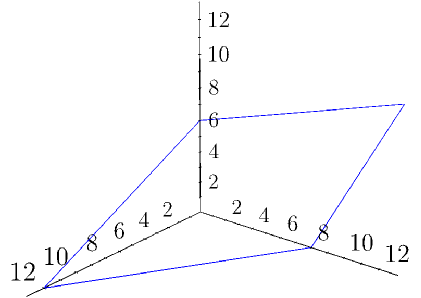
\includegraphics[width=\linewidth]{generated/asymptote/fig-plane-2.pdf}
\end{image}%
\tcblower
\end{figureptx}%
We will encounter inequalities involving three variables. As seen in two dimensions, the feasible set will be the set of all points satisfying all of inequalities. It is difficult to graph this, but one can imagine that in three dimensions, the same ideas hold as those above. For example, one can cross out the side of the plane that is not in the feasible set and then the region in \(\mathbb{R}^3\) is the region not crossed out.%
\begin{figureptx}{Figure}{A plot of a feasible set of in \(\mathbb{R}^3\).  If this is being viewed in a web browser, the graph should be interactive in that it can be rotated.}{fig-plane-2}{}%
\begin{image}{0}{1}{0}{}%
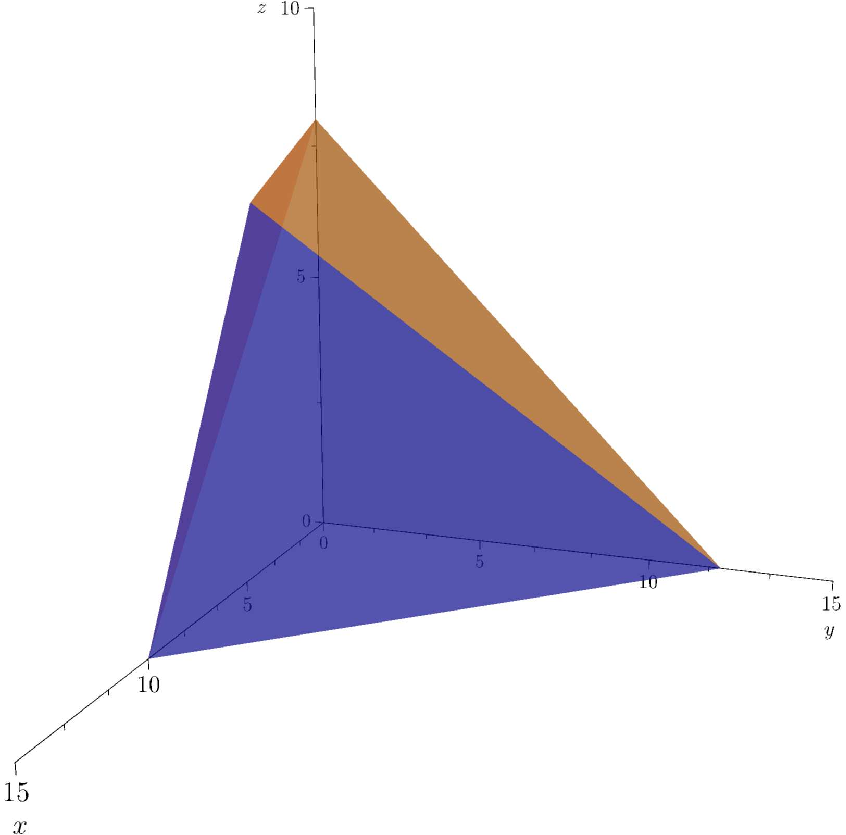
\includegraphics[width=\linewidth]{generated/asymptote/fig-plane-2-2.pdf}
\end{image}%
\tcblower
\end{figureptx}%
Linear equations with more than 3 variables are often called \terminology{hyperplanes.} Although impossible to graph, these work the same ways as lines and planes in that the cut the Euclidean space in half.%
\end{subsectionptx}
%
%
\typeout{************************************************}
\typeout{Subsection 1.1.5 Convex Sets}
\typeout{************************************************}
%
\begin{subsectionptx}{Subsection}{Convex Sets}{}{Convex Sets}{}{}{sect-convex}
As we will see later, a convex feasible set is key to the simplex method working. What does \emph{convex} mean? We will explore this and show that a feasible set constructed of linear inequalities is always convex.%
\begin{definition}{Definition}{}{def-convex}%
A set \(S\) in \(\mathbb{R}^n\) is \terminology{convex} if for any two points \(\boldsymbol{x}\) and \(\boldsymbol{y}\) in \(S\) that all points in the line segment connecting \(\boldsymbol{x}\) and \(\boldsymbol{y}\) is in \(S\)%
\end{definition}
\begin{note}{Note}{}{sect-convex-4}%
Note: a line segment between points \(\boldsymbol{x}\) and \(\boldsymbol{y}\) can be written%
\par
%
\begin{equation*}
L = \{ \boldsymbol{x} t + \boldsymbol{y} (1-t) \; | \; t \in [0,1]\}.
\end{equation*}
%
\end{note}
In two dimensions, a convex set is a set in \(\mathbb{R}^2\) such that its boundary is convex in the standard sense. Sets like the interior of circles, rectangles and the ``inside'' of parabolas are examples. To get a sense of this, the sets consisting of the interior of the following objects are convex:%
\begin{figureptx}{Figure}{Examples of convex sets (interiors of circles and polygons).  Example line segments are shown within the figures.}{fig-convex-objects}{}%
\begin{image}{0.125}{0.75}{0.125}{}%
\resizebox{\linewidth}{!}{%
\begin{tikzpicture}
  \draw (0,0) rectangle (4,3);
  \draw (5,0) -- (7,3) -- (9,0) -- cycle;
  \draw (12,2) circle [radius = 2];
  \draw[thick, blue] (0.25,0.5) -- (3.5,2);
  \draw[thick, blue] (7.5,0.5) -- (6.7,2);
  \draw[thick,blue] (11.5,1.8) -- (13,1.1);
\end{tikzpicture}%
}%
\end{image}%
\tcblower
\end{figureptx}%
Although example line segments are shown drawn within the figures in \hyperref[fig-convex-objects]{Figure~{\xreffont\ref{fig-convex-objects}}}, recall that in order to be convex, all line segments need to be within the set, not just an example line segment.%
\par
However, the interior of the objects in \hyperref[fig-non-convex-objects]{Figure~{\xreffont\ref{fig-non-convex-objects}}} are not. A line is shown in blue with point endpoints that are in the set, but the are parts of the line that are not in the set.%
\begin{figureptx}{Figure}{The interior of these shapes are not convex.  Example line segments are drawn which have points that are outside the shape (sets).}{fig-non-convex-objects}{}%
\begin{image}{0.125}{0.75}{0.125}{}%
\resizebox{\linewidth}{!}{%
\begin{tikzpicture}
   \draw (0,3) -- (2,0.5) -- (4,3) -- (2,0) -- cycle;
  \draw (5,2) arc[start angle = 180, end angle = 360, radius = 2] --
  (9,2) arc[start angle = 0, end angle = 180, radius = 0.75] --
  (7.5,2) arc[start angle = 360, end angle = 180, radius = 0.5] --
  (6.5, 2) arc[start angle = 0, end angle = 180, radius= 0.75] -- cycle;
 \draw[thick, blue] (6,2.2) -- (8,2);
 \draw[thick,blue ] (1.4,1) -- (2.95,1.5);
\end{tikzpicture}%
}%
\end{image}%
\tcblower
\end{figureptx}%
The next lemma states the seemingly obvious fact that splitting the plane with a linear inequality results in a convex set.%
\begin{lemma}{Lemma}{}{}{lem-convex-one-inequality}%
Let \(S = \{ (x,y) \; | \; a x + b y \leq c \}\) with \(a, b, c \in \mathbb{R}\) and \(ab \neq 0\). The set \(S\) is convex.%
\end{lemma}
\begin{proof}{Proof}{}{lem-convex-one-inequality-2}
Let \((x_1, y_1)\) and \((x_2, y_2)\) be two points in \(S\). The line segment between them is the parametric equation%
\par
%
\begin{equation*}
x(t) = x_1 t + (1-t) x_2 \qquad y(t) = y_1 t + (1-t) y_2.
\end{equation*}
%
\par
To show convexity, the line segment must be in \(S\). That is,%
\par
%
\begin{align*}
a (x_1 t + (1-t) x_2) + b(y_1 t + (1-t)y_2) \amp = t (a x_1 + b y_1) + (1-t) (a x_2 + b y_2) \\
\amp \leq tc + (1-t) c \\
\amp = tc+c-ct = c
\end{align*}
%
\par
And since the both points \((x_1,y_1)\) and \((x_2, y_2)\) are in \(S\), then \(a (x_1 t + (1-t) x_2) + b(y_1 t + (1-t)y_2) \leq c\), the line segment is in \(S\), therefore the set is convex.%
\end{proof}
This showed that the linear inequality in \(\mathbb{R}^2\) is convex, however this is true in any dimension.%
\begin{lemma}{Lemma}{}{}{lem-lin-inequality-Rn}%
Let \(\boldsymbol{x} = (x_1, x_2, \ldots, x_n)\) and \(S = \{ \boldsymbol{x} \; | \; a_1 x_1 + a_2 x_2 + \cdots a_n x_n \leq c \}\) for \(a_1, a_2, \ldots, a_n, c\) constants. The set \(S\) is convex.%
\end{lemma}
This lemma is the first step in showing the general convexity of more complex sets. The next one will give the next step.%
\begin{lemma}{Lemma}{}{}{sect-convex-15}%
Let \(S\) and \(T\) be two convex sets. The intersection \(S \cap T\) is convex.%
\end{lemma}
The proof is left to the reader.%
\end{subsectionptx}
\end{sectionptx}
%
%
\typeout{************************************************}
\typeout{Section 1.2 Using Software for Plotting}
\typeout{************************************************}
%
\begin{sectionptx}{Section}{Using Software for Plotting}{}{Using Software for Plotting}{}{}{sect-plotting-software}
\begin{objectives}{Objectives}{sect-plotting-software-2}
%
\begin{itemize}[label=\textbullet]
\item{}Using Desmos or other software to plot lines and linear inequalities.%
\end{itemize}
\end{objectives}
%
%
\typeout{************************************************}
\typeout{Subsection 1.2.1 Plotting Lines}
\typeout{************************************************}
%
\begin{subsectionptx}{Subsection}{Plotting Lines}{}{Plotting Lines}{}{}{sect-plotting-lines}
Software can help with the plotting of lines, planes and linear inequalities. In \hyperref[sect-lines]{Subsection~{\xreffont\ref{sect-lines}}}, the equation \(3x+4y=12\) and linearly inequality \(3x+4y \leq 12\) was plotted.%
\par
Visit \href{https://www.desmos.com/calculator}{Desmos} which will look like:%
\begin{figureptx}{Figure}{}{fig-desmos}{}%
\begin{image}{0}{1}{0}{}%
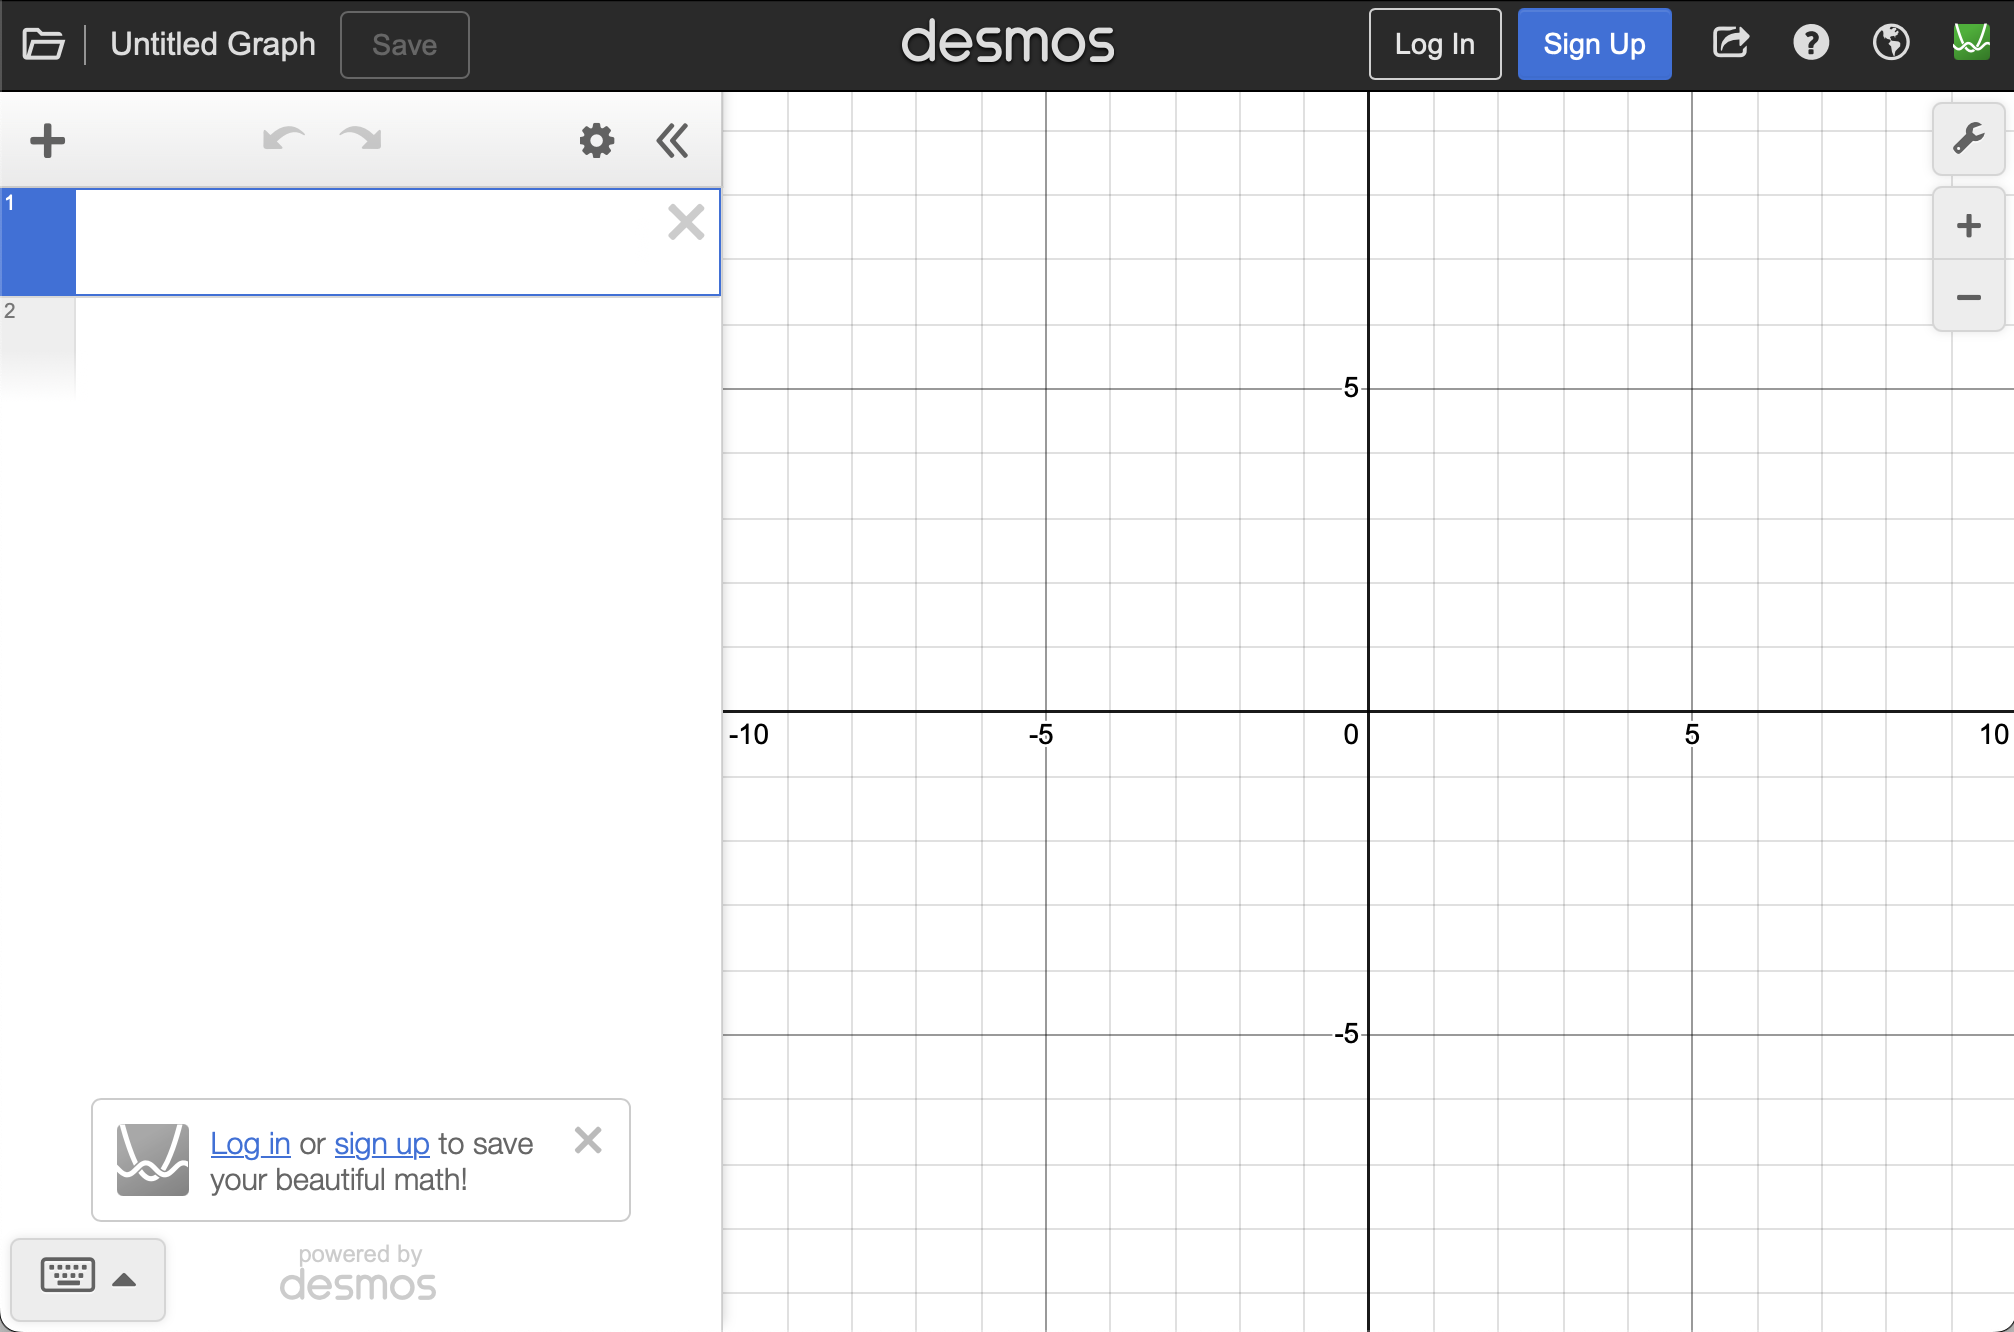
\includegraphics[width=\linewidth]{external/images/desmos.png}
\end{image}%
\tcblower
\end{figureptx}%
Enter \mono{3x+4y=12} in the first box (outlined in blue) and you should see%
\begin{figureptx}{Figure}{}{fig-desmos-line-plot}{}%
\begin{image}{0}{1}{0}{}%
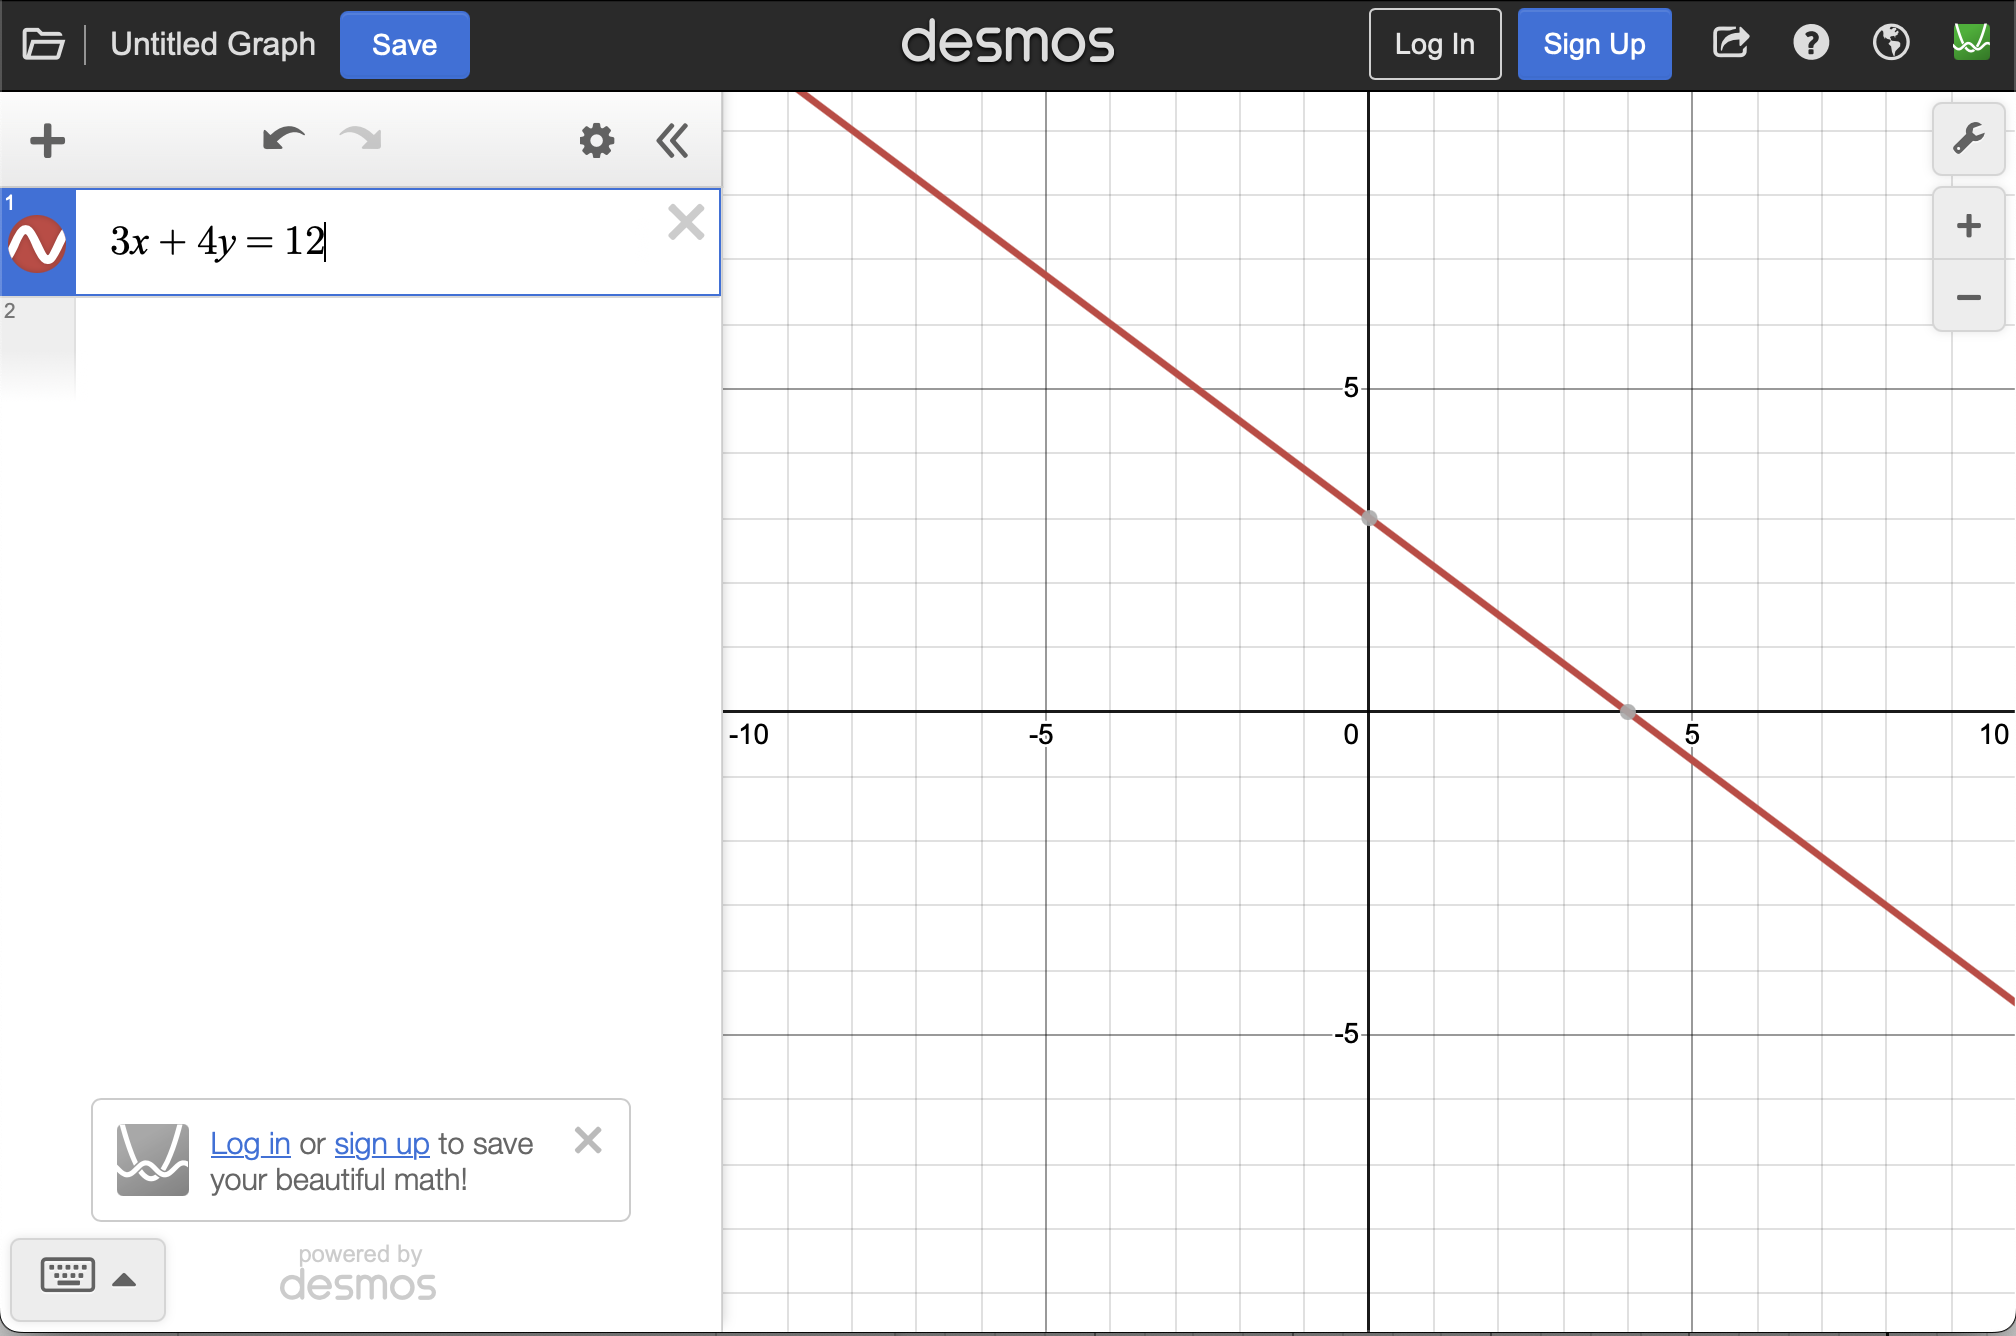
\includegraphics[width=\linewidth]{external/images/desmos-line-plot.png}
\end{image}%
\tcblower
\end{figureptx}%
Additional lines can be plotted by adding them to the box below the previous line. For example, enter \mono{y=2x=3} results in%
\begin{figureptx}{Figure}{}{fig-desmos-two-lines}{}%
\begin{image}{0}{1}{0}{}%
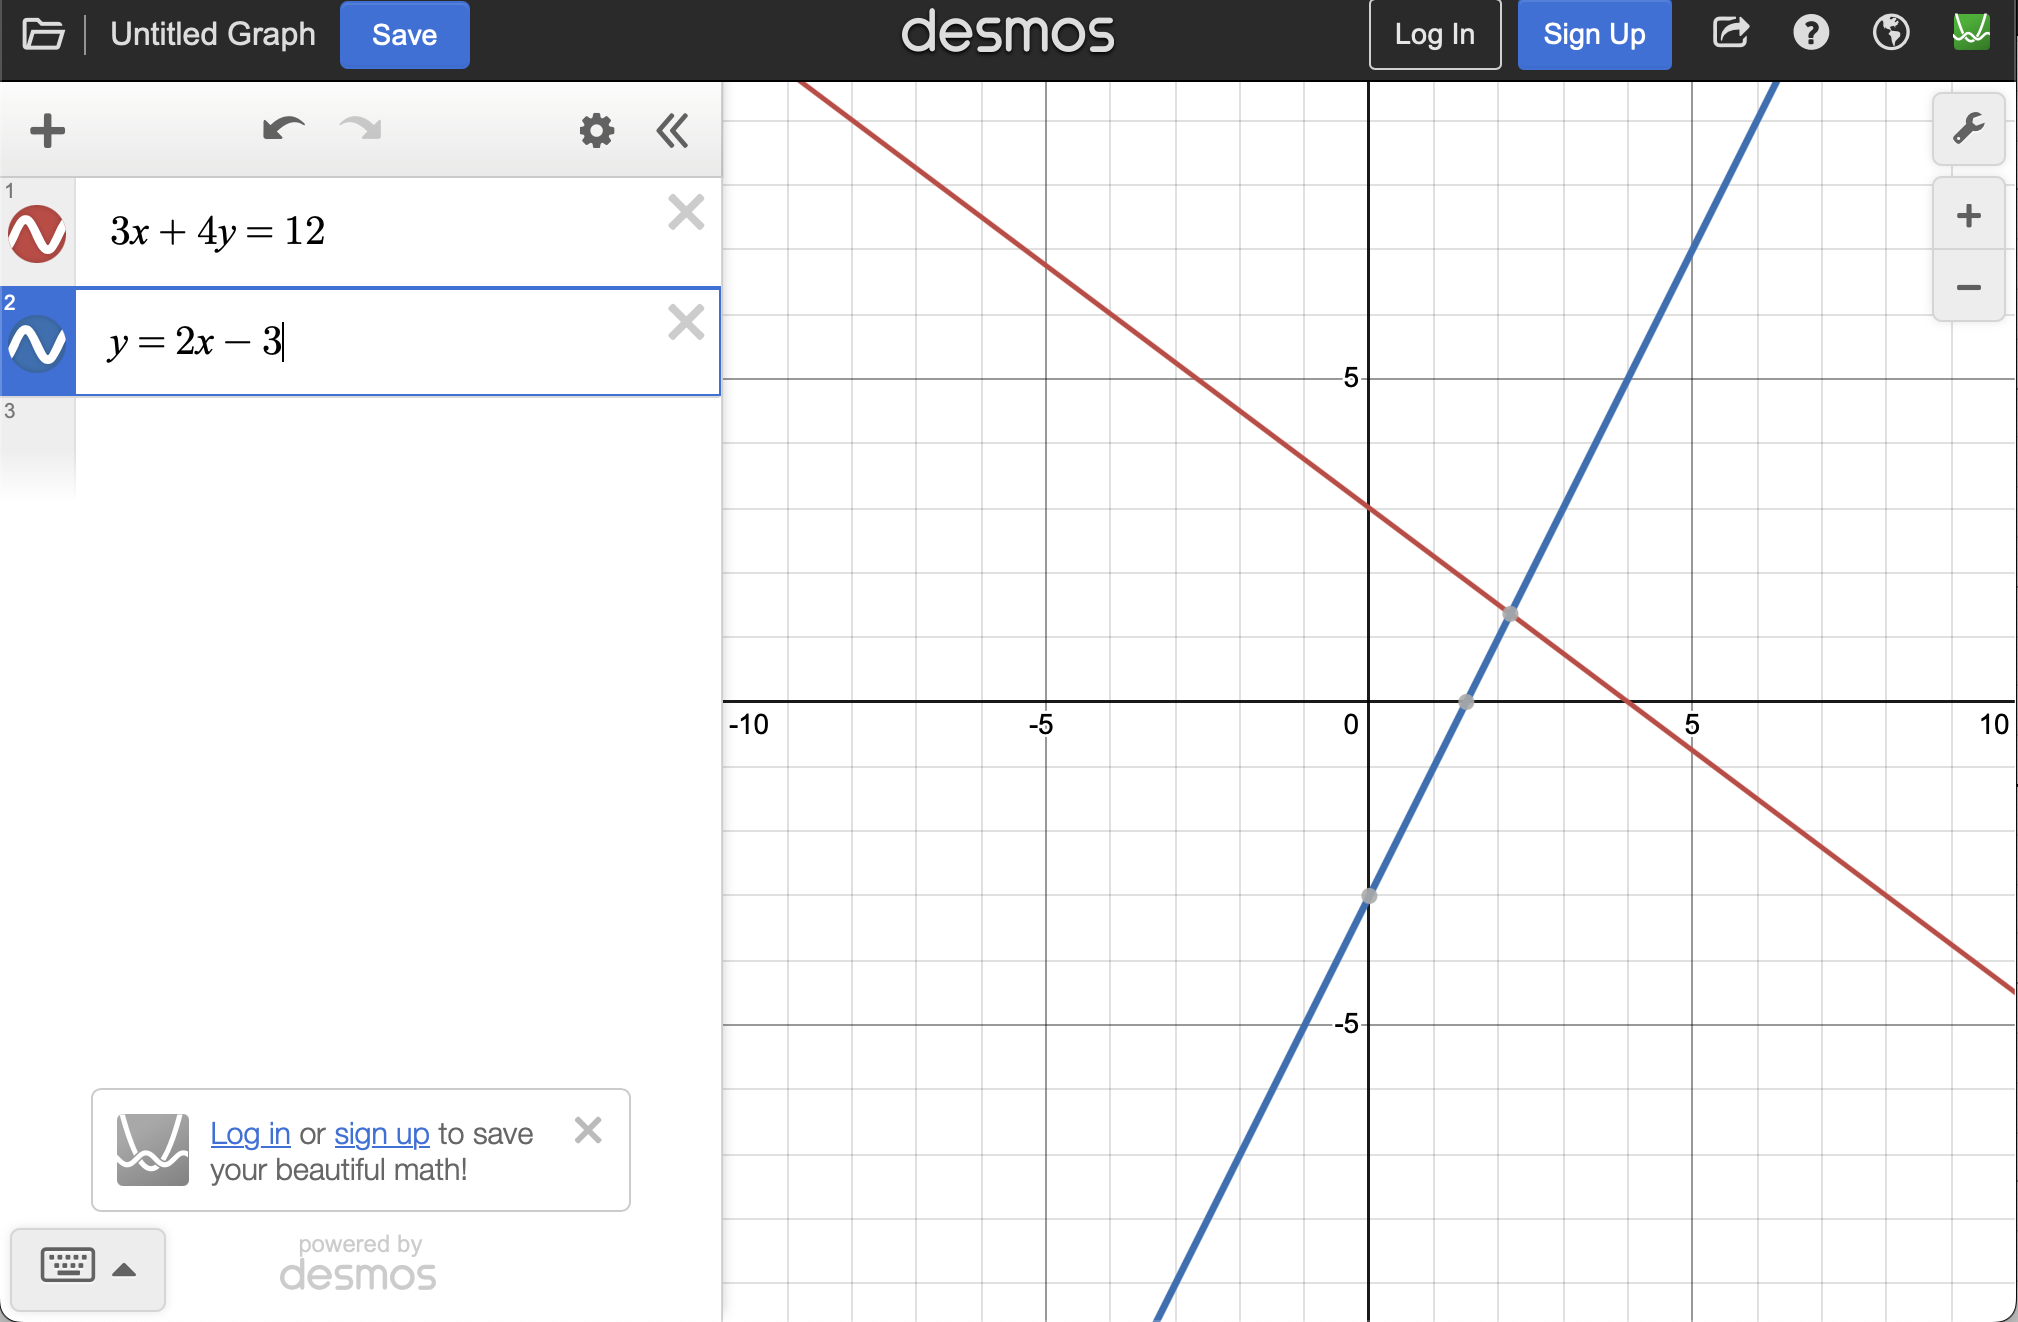
\includegraphics[width=\linewidth]{external/images/desmos-two-lines.png}
\end{image}%
\tcblower
\end{figureptx}%
\end{subsectionptx}
%
%
\typeout{************************************************}
\typeout{Subsection 1.2.2 Plotting Inequalities and Feasible Sets}
\typeout{************************************************}
%
\begin{subsectionptx}{Subsection}{Plotting Inequalities and Feasible Sets}{}{Plotting Inequalities and Feasible Sets}{}{}{sect-plotting-inequalities}
Inequalities can also be plotted. Return to desmos and remove all equations by hitting the X on the right side of each entry box. Now add \mono{3x+4y ≤ 12} where Demos will automatically convert \mono{<=} to \mono{≤}. The resulting plot will be%
\begin{figureptx}{Figure}{}{fig-desmos-inequality}{}%
\begin{image}{0}{1}{0}{}%
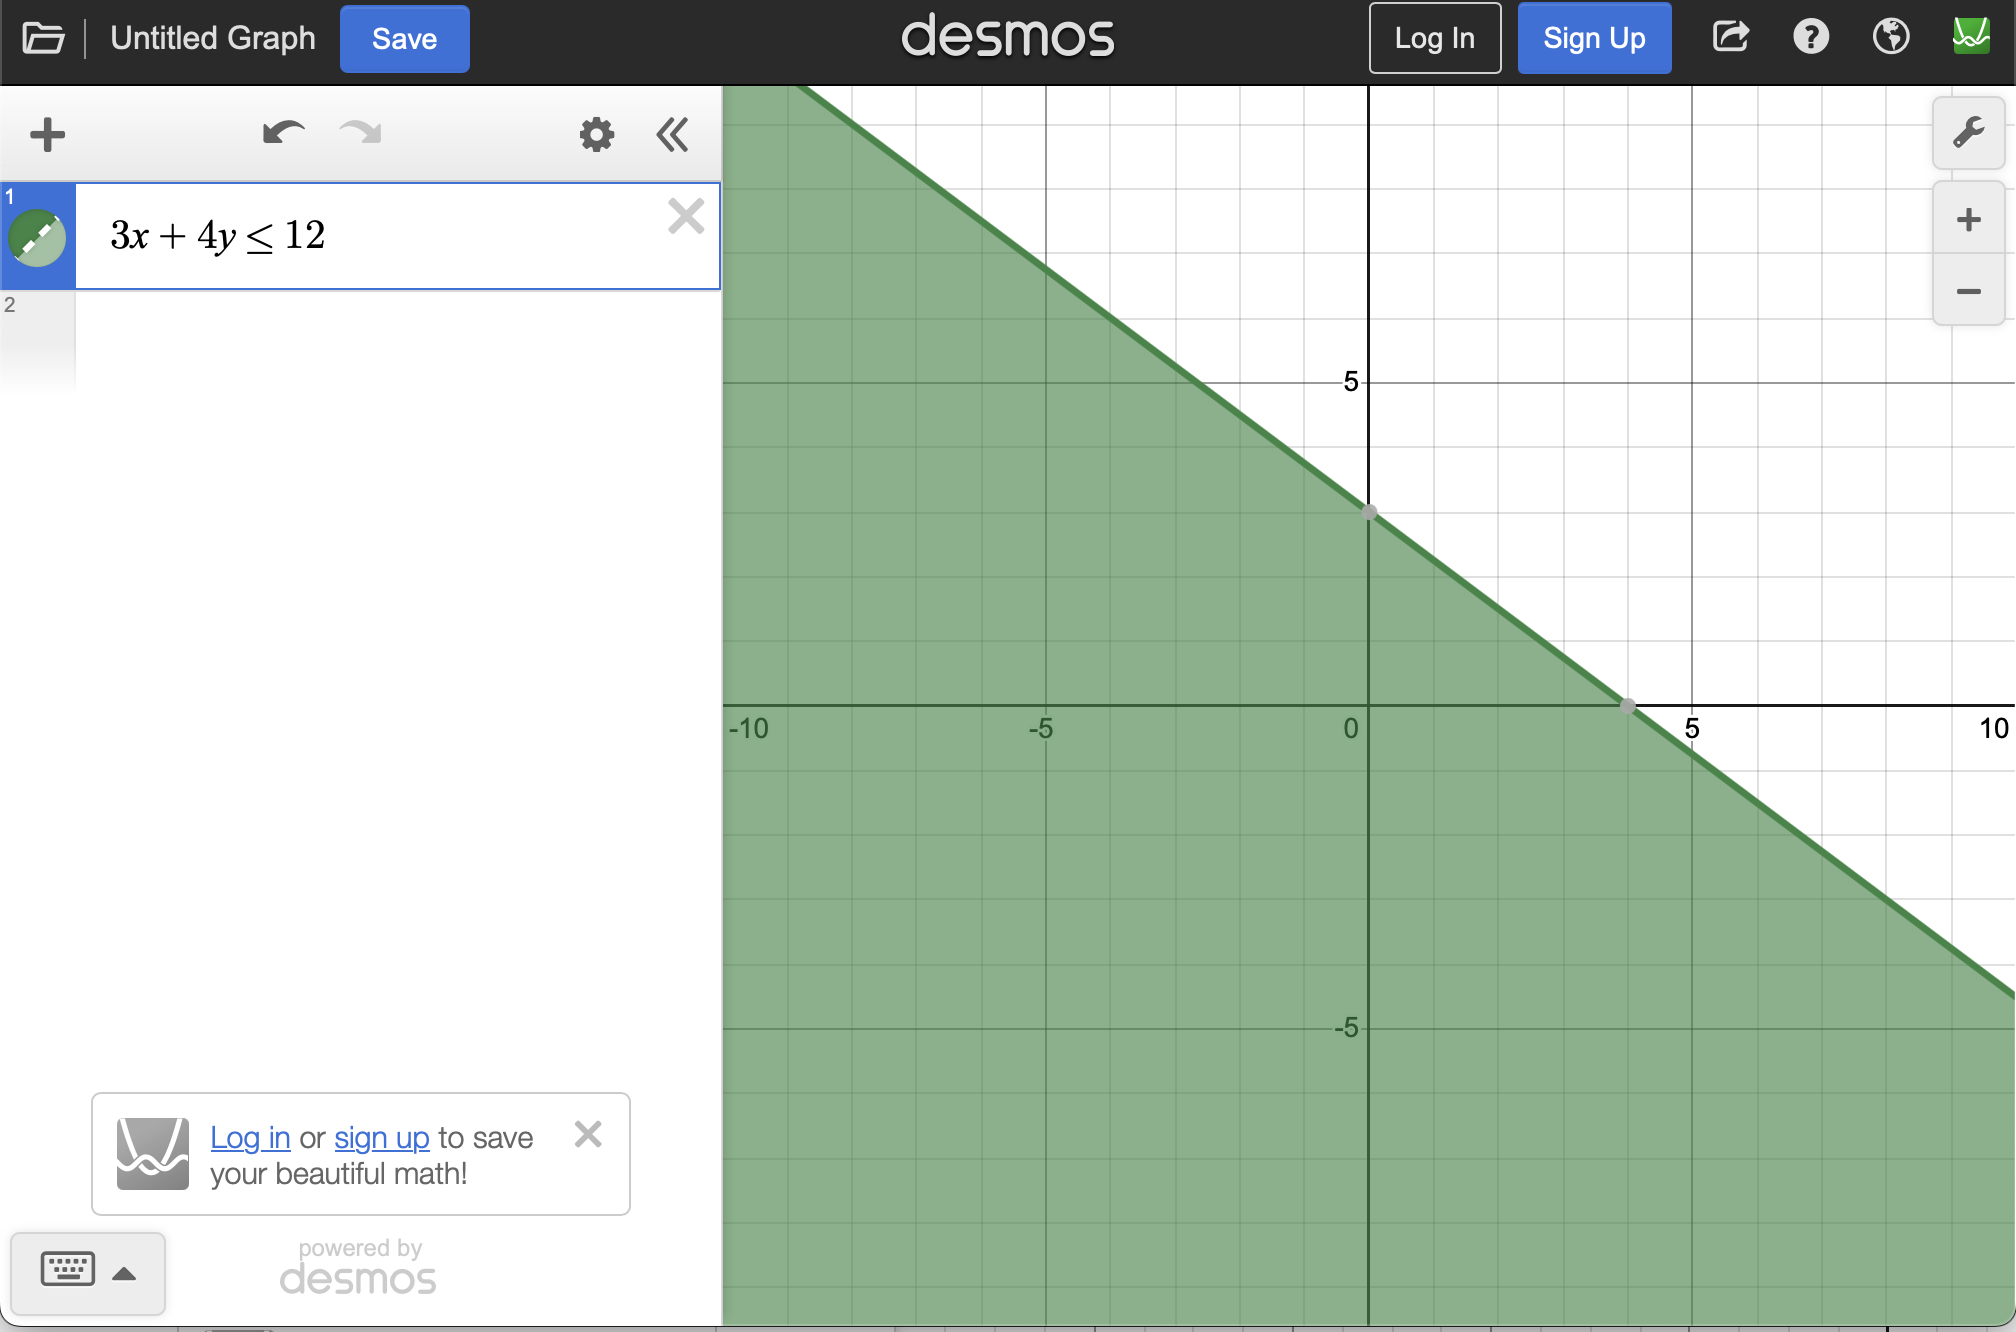
\includegraphics[width=\linewidth]{external/images/desmos-inequality.png}
\end{image}%
\tcblower
\end{figureptx}%
Note that the colors of all the plots may be different. Desmos usually cycles through the colors in a specific manner, but this may differ as you enter equations.%
\par
The graph shows both the line as solid and the color as a light green indicating that the region below and left of the line is part of the inequality.%
\par
This idea can be extended to plotting sets of inequalities to arrive at a feasible set. Recall that in \hyperref[sect-lines-planes]{Section~{\xreffont\ref{sect-lines-planes}}} the set of inequalities:%
\par
%
\begin{align*}
3x+4y \amp \leq 12 \\
y \amp \geq x+1
\end{align*}
%
\par
was plotted. If we add the second inequality to Demos we get%
\begin{figureptx}{Figure}{}{fig-desmos-two-inequalities}{}%
\begin{image}{0}{1}{0}{}%
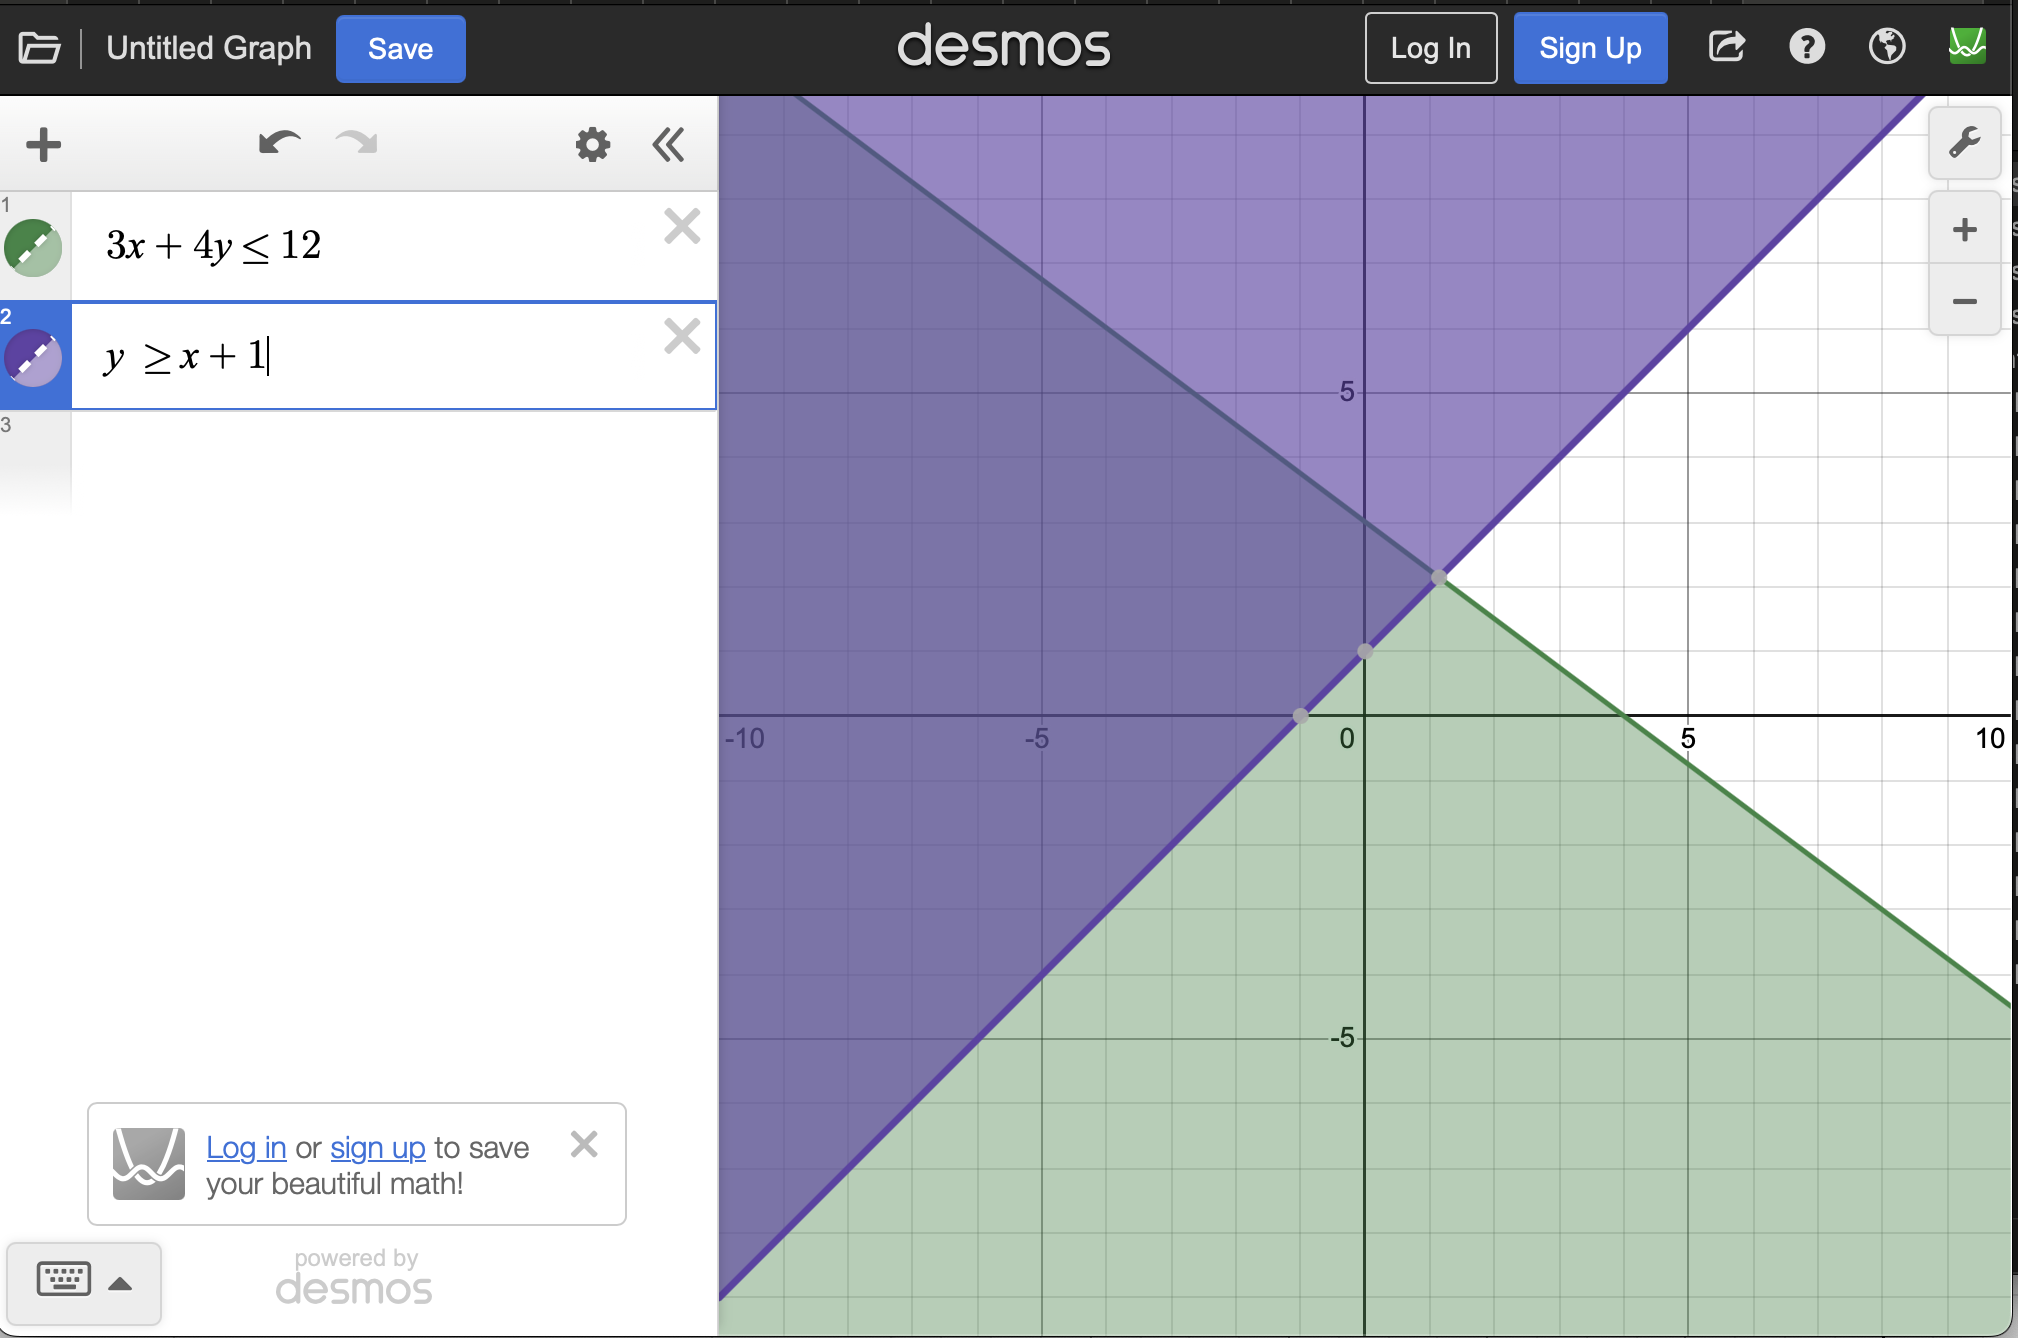
\includegraphics[width=\linewidth]{external/images/desmos-two-inequalities.png}
\end{image}%
\tcblower
\end{figureptx}%
With only two inequalities, visually the overlap (the set of points that satisfy both inequalities) is reasonably easy to see, however, as these grow, it can be more difficulty to see. One way is to plot the opposite inequality and then area of the plane with no coloring would be the resultant set.%
\begin{example}{Example}{}{sect-plotting-inequalities-11}%
Use Desmos to plot the region that satisfies the following:%
\par
%
\begin{equation*}
\begin{aligned} x - 2y \leq -2, \\ 5x-2y \geq 15, \\ 3x+5y \geq 75. \end{aligned}
\end{equation*}
%
\par\smallskip%
\noindent\textbf{\blocktitlefont Solution}.\hypertarget{sect-plotting-inequalities-11-2}{}\quad{}We open up Desmos and add all three of the inequalities, except switching each inequality. The result is%
\begin{figureptx}{Figure}{}{fig-desmos-three-inequalities}{}%
\begin{image}{0}{1}{0}{}%
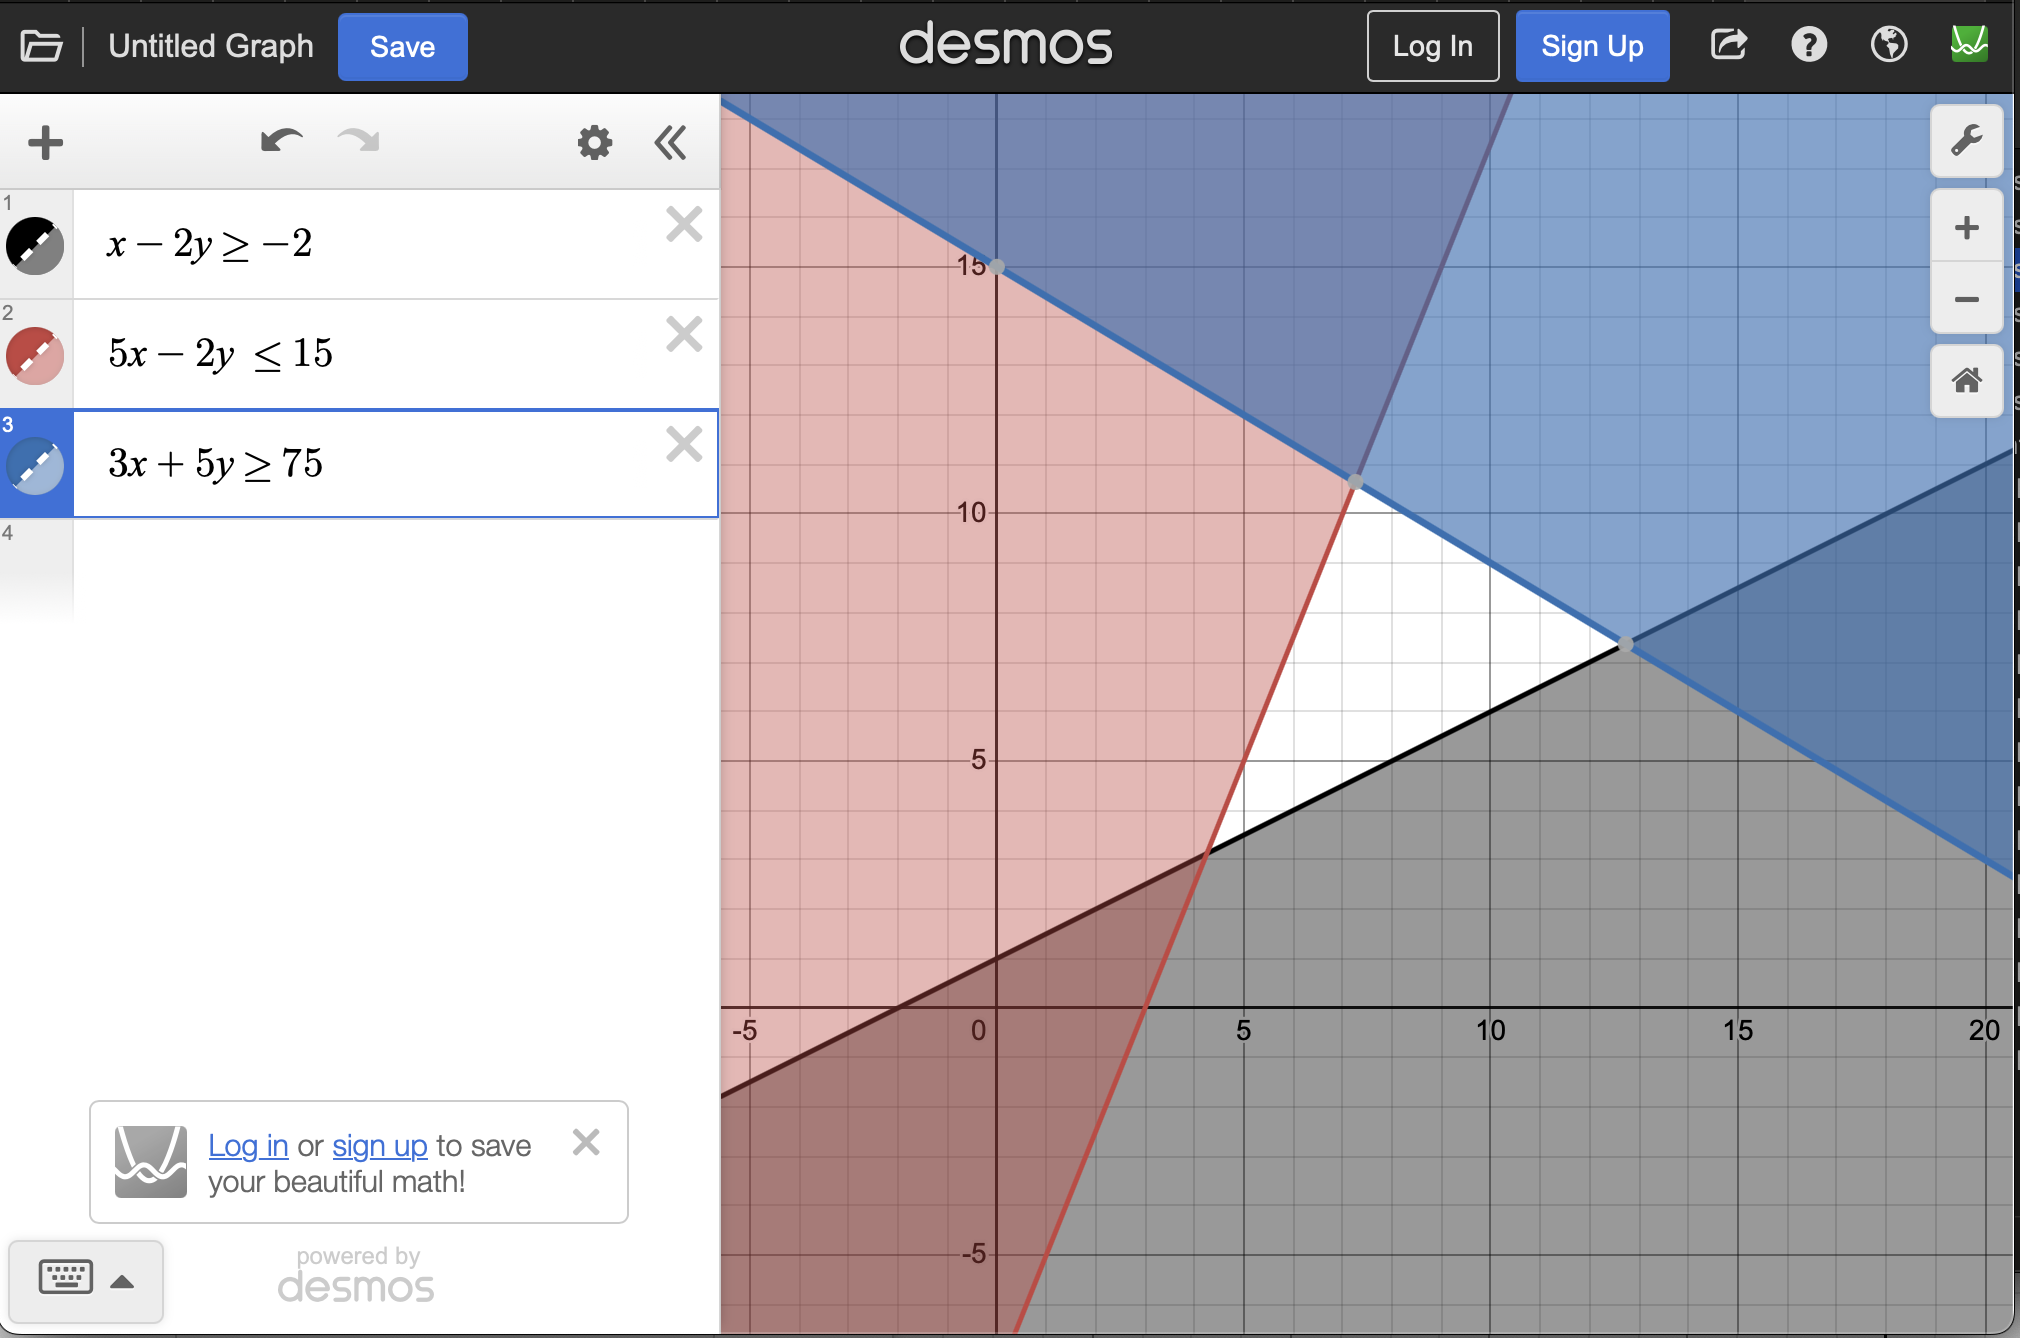
\includegraphics[width=\linewidth]{external/images/desmos-three-inequalities.png}
\end{image}%
\tcblower
\end{figureptx}%
The set of points that satisfy the three inequalities is the triangular region without any shading.%
\end{example}
\end{subsectionptx}
%
%
\typeout{************************************************}
\typeout{Subsection 1.2.3 Graphing Planes}
\typeout{************************************************}
%
\begin{subsectionptx}{Subsection}{Graphing Planes}{}{Graphing Planes}{}{}{sect-graphing-planes}
As we saw in \hyperref[sect-lines-planes]{Section~{\xreffont\ref{sect-lines-planes}}}, planes are another example of linear functions that we will encounter in this text.  Desmos also has a \href{https://www.desmos.com/3d}{3D graphing calculator}.   Open up the webpage and it will look like the regular graphing calculator, however the default axes are in \(\mathbb{R}^3\).%
\par
Add \mono{x+2y+3z=12} to the plot and you should get a plane.  Spin the axes around and zoom in and out with the + and - buttons.  You may get something that looks like%
\begin{figureptx}{Figure}{}{fig-desmos-plane}{}%
\begin{image}{0}{1}{0}{}%
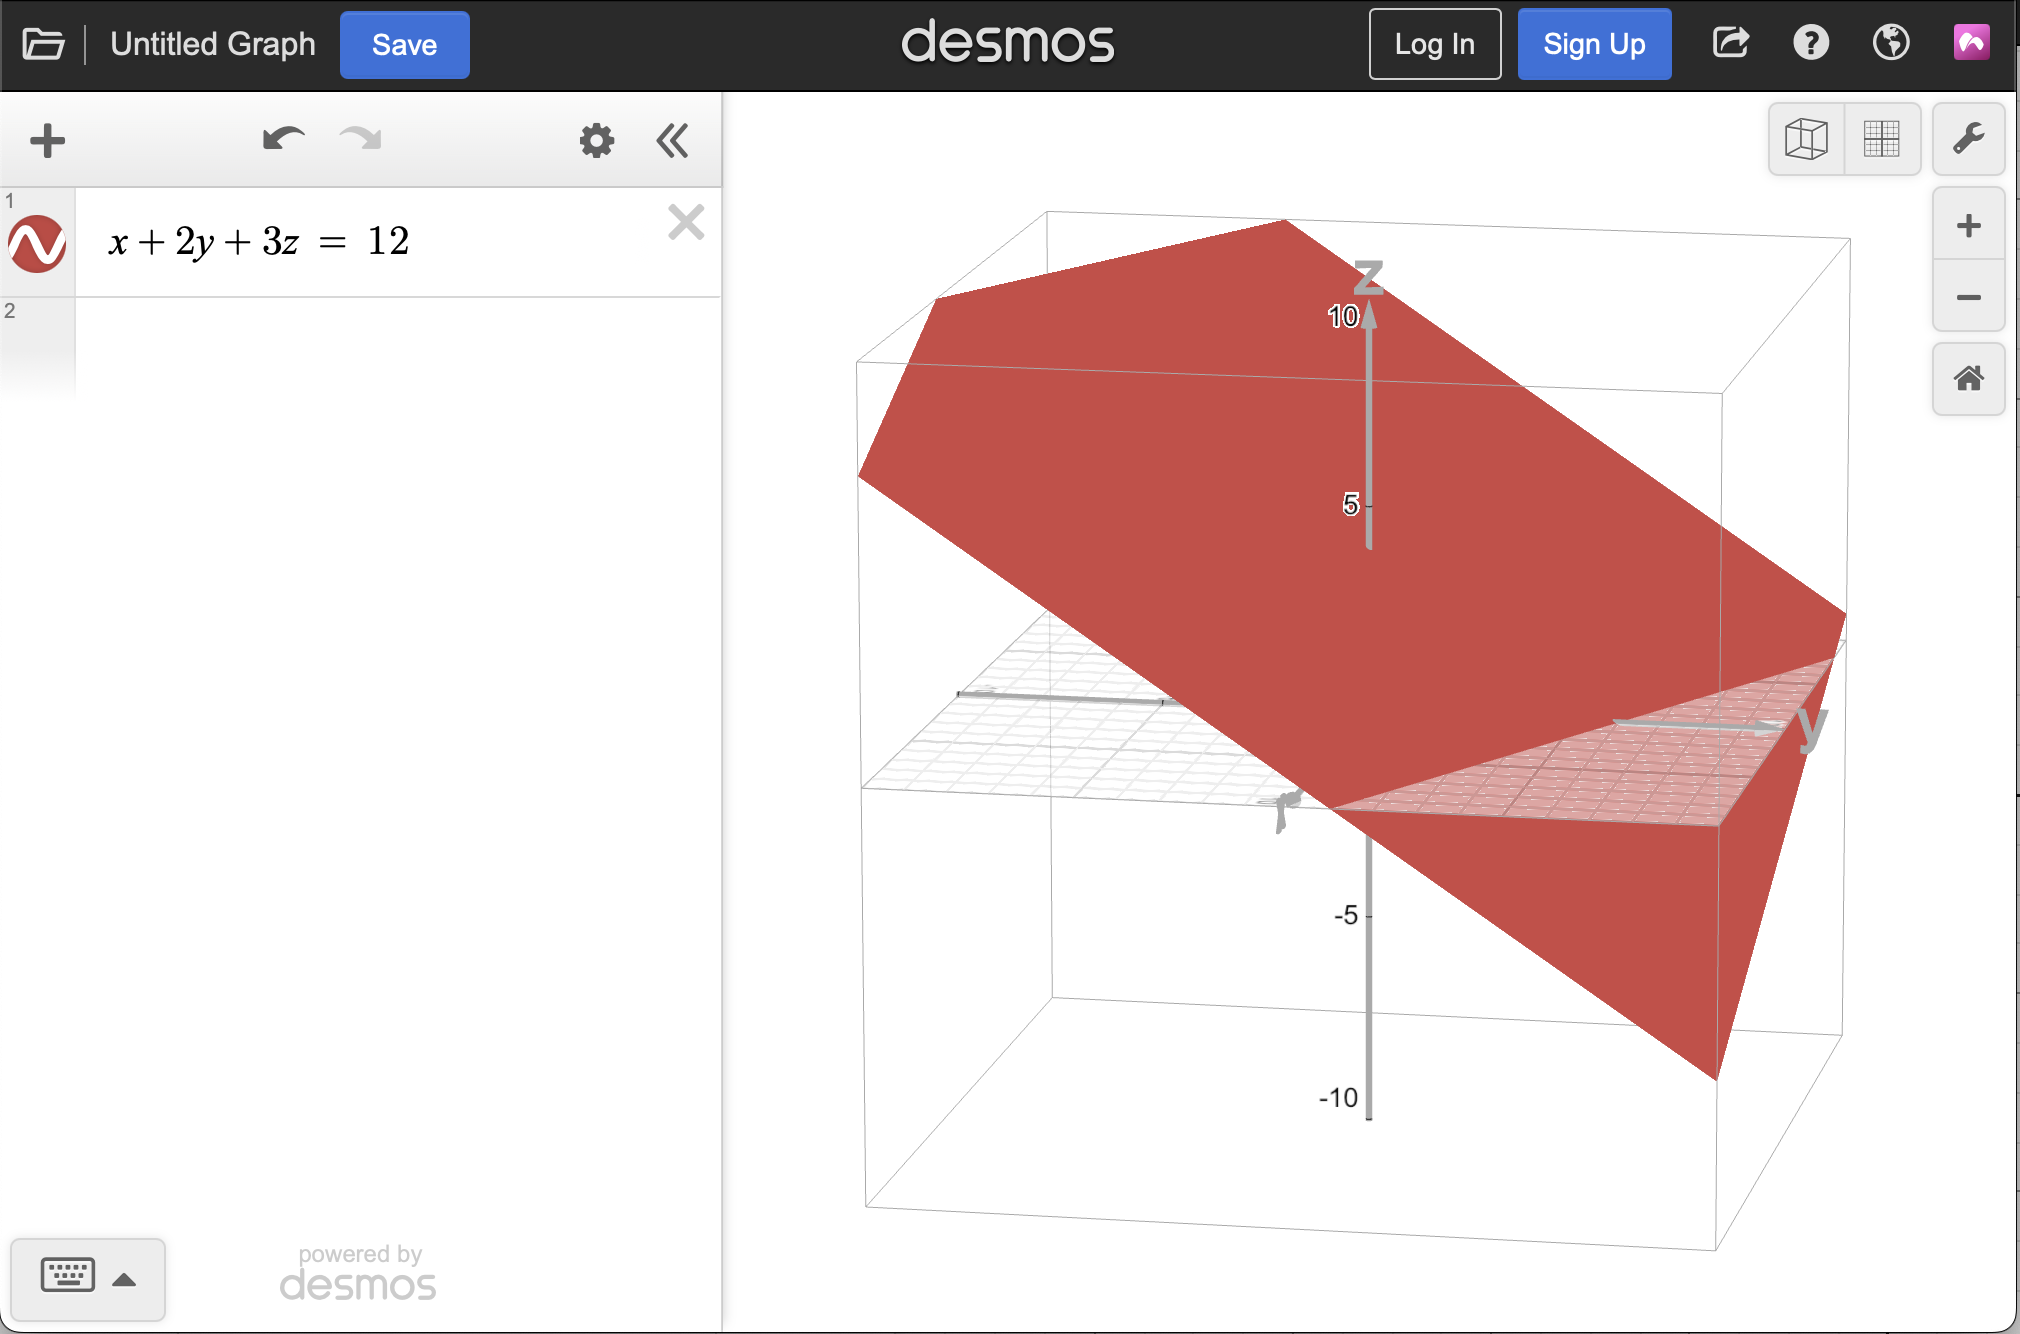
\includegraphics[width=\linewidth]{external/images/desmos-plane.png}
\end{image}%
\tcblower
\end{figureptx}%
Inequalities can also be plotted, however, they are difficult to read.  For example, change the \(=\) in the previous plane to a \(\leq\) or \(\geq\) and you will see that half of the \(\mathbb{R}^3\) space is now colored red (in my case). However, adding another inequality will be quite difficult to see the intersecting region.%
\end{subsectionptx}
\end{sectionptx}
%
%
\typeout{************************************************}
\typeout{Section 1.3 Matrices and Matrix Reduction}
\typeout{************************************************}
%
\begin{sectionptx}{Section}{Matrices and Matrix Reduction}{}{Matrices and Matrix Reduction}{}{}{sect-matrix-reduction}
\begin{introduction}{}%
Matrices are generally presented in either a linear algebra or matrix methods class. The material presented here is some basics behind matrices that are needed for performing linear optimization. This should be review for most readers of the text, but is helpful for the context and notation later in the text.%
\end{introduction}%
%
%
\typeout{************************************************}
\typeout{Subsection 1.3.1 Linear Systems}
\typeout{************************************************}
%
\begin{subsectionptx}{Subsection}{Linear Systems}{}{Linear Systems}{}{}{sect-linear-systems}
Let's start with an example.%
\begin{example}{Example}{Traffic Flow.}{ex-streets}%
A simple model of traffic flow can be represented by the following graph:%
\begin{figureptx}{Figure}{A map of a few streets in Boston where the arrows denote the direction of traffic flow (all of these streets are one-way) and the numbers represent the numbers of cars driving down the street in a given time period. The letters \(A\) through \(D\) will be the names of the intersections.}{fig-streets}{}%
\begin{image}{0.125}{0.75}{0.125}{}%
\resizebox{\linewidth}{!}{%
\begin{tikzpicture}[scale=1.5] \draw[{Latex[length=2mm]}-] (0,1) -- (2,1) node [at start,below left] {Newbury St.}; \draw[-{Latex[length=2mm]}] (0,0) -- (3,0) node [at end,above right] {Bolyston St.} ; \draw[{Latex[length=2mm]}-] (1,2) -- (1,-1) node [at start,above left=5pt+3pt] {Berkeley St.}; \draw[{Latex[length=2mm]}-] (2,-1) -- (2,2) node [at end,above right=5pt+3pt] {Arlington St.} ; \draw[{Latex[length=2mm]}-] (2,1.5) -- (2,1.6); \draw[{Latex[length=2mm]}-] (2,0.5) -- (2,0.6); \draw[-{Latex[length=2mm]}] (1,-0.5) -- (1,-0.4); \draw[-{Latex[length=2mm]}] (1,0.5) -- (1,0.6); \draw[{Latex[length=2mm]}-] (0.5,0) -- (0.4,0); \draw[{Latex[length=2mm]}-] (1.5,0) -- (1.4,0); \draw[{Latex[length=2mm]}-] (1.5,1) -- (1.6,1); \draw (3,0) node [below right] {400}; \draw (2,-1) node [below right] {200}; \draw (0,0) node [above left] {500}; \draw (1,-1) node [below left] {200}; \draw (0,1) node [above left] {$ x_1$}; \draw (1,2) node [above] {250}; \draw (2,2) node [above] {350}; \draw (1.5,0) node [below] {$ x_2$}; \draw (2,0.5) node [right] {$ x_3$}; \draw (1.5,1) node [above] {$ x_4$}; \draw (1,0.5) node [left] {$ x_5$}; \fill (1,1) circle[radius=1.5pt] node [above left] {$ A$}; \fill (2,1) circle[radius=1.5pt] node [above right] {$ B$}; \fill (1,0) circle[radius=1.5pt] node [above right] {$ C$}; \fill (2,0) circle[radius=1.5pt] node [below right] {$ D$}; \end{tikzpicture}%
}%
\end{image}%
\tcblower
\end{figureptx}%
Write down the equations that balance each of the numbers of cars entering and leaving each of the intersections \(A, B, C\) and \(D\).%
\par\smallskip%
\noindent\textbf{\blocktitlefont Solution}.\hypertarget{ex-streets-3}{}\quad{}In this case, we have:%
\par
%
\begin{equation}
\begin{aligned} x_4 + x_5 \amp = x_1 + 250 350 \amp = x_3 + x_4 700 \amp = x_2 + x_5 x_3 + x_2 \amp = 600 \end{aligned}\label{eq-traffic}
\end{equation}
%
\par
for intersections \(A\), \(B\), \(C\) and \(D\) respectively.%
\end{example}
\begin{definition}{Definition}{}{sect-linear-systems-4}%
%
\begin{itemize}[label=\textbullet]
\item{}A \terminology{linear combination} of \(x_1, x_2, x_3, \ldots, x_n\) has the form%
\par
%
\begin{equation*}
a_1 x_1 + a_2 x_2 + \cdots + a_n x_n,
\end{equation*}
%
\par
where the constants \(a_1, a_2, \ldots, a_n \in \mathbb{R}\) are the combinations coefficients.%
\item{}A \terminology{linear equation} has the form%
\par
%
\begin{equation}
a_1 x_1 + a_2 x_2 + \cdots + a_n x_n = b\label{eq-def-lin-eq}
\end{equation}
%
\par
where \(b \in \mathbb{R}\) is a constant and \(a_1, a_2, \ldots, a_n \in \mathbb{R}\). These are the lines, planes and hyperplanes discussed in \hyperref[sect-lines-planes]{Section~{\xreffont\ref{sect-lines-planes}}}.%
\item{}The \(n\)-tuple \((s_1,s_2,\ldots,s_n)\) \terminology{satisfies} or is a \terminology{solution} of \hyperref[eq-def-lin-eq]{({\xreffont\ref{eq-def-lin-eq}})} if this point satisfies \hyperref[eq-def-lin-eq]{({\xreffont\ref{eq-def-lin-eq}})} or%
\par
%
\begin{equation*}
a_1 s_1 + a_2 s_2 + \cdots + a_n s_n = b
\end{equation*}
%
\item{}A \terminology{system of linear equations} or \terminology{linear system} is a set of linear equations:%
\par
%
\begin{align}
a_{1,1} x_1 + a_{1,2} x_2 + \cdots + a_{1,n} x_n \amp = b_1 , \notag\\
a_{2,1} x_1 + a_{2,2} x_2 + \cdots + a_{2,n} x_n \amp = b_2, \label{eq-def-lin-sys}\\
\vdots \amp = \vdots \notag\\
a_{m,1} x_1 + a_{m,2} x_2 + \cdots + a_{m,n} x_n \amp = b_m, \notag
\end{align}
%
\par
and this linear system has \(m\) equations and \(n\) unknowns (variables). The equations in \hyperref[eq-traffic]{({\xreffont\ref{eq-traffic}})} is an example of a linear system.%
\item{}The \(n\)-tuple \((s_1,s_2,\ldots,s_n)\) \terminology{satisfies} or is a \terminology{solution} of \hyperref[eq-def-lin-sys]{({\xreffont\ref{eq-def-lin-sys}})} if this point satisfies \emph{every} equation of \hyperref[eq-def-lin-sys]{({\xreffont\ref{eq-def-lin-sys}})}.%
\end{itemize}
%
\end{definition}
\begin{example}{Example}{Linear Equations.}{sect-linear-systems-5}%
The following are linear equations:%
\par
%
\begin{align*}
2x + 3y \amp = 6, \amp y_1 -y_2+y_3-y_4 \amp = 10, \\
10x_1 - x_3 + 5x_5 \amp = 9, \amp \sum_{i=1}^{10} i x_i \amp = 0
\end{align*}
%
\par
where summation notation has been used in the last one and note the variable names can vary. The following equations are not linear:%
\par
%
\begin{align*}
x_1^2+x_2 \amp = 6, \amp y_1y_2 + y_3 \amp = 5, \\
\frac{x_1+x_2}{x_3} \amp = 6, \amp \sin(x+y) \amp = z
\end{align*}
%
\par
Each of the equations in the latter group have multiplications, squares, division or other functions between variables.%
\end{example}
The next two examples give a way to determine if a point or \(n\)-tuple is a solution to a linear system.%
\begin{example}{Example}{Showing a Point is a Solution to a Linear System.}{sect-linear-systems-7}%
Show that the point \((2,3)\) is a solution of the linear system:%
\par
%
\begin{align*}
3x_1 - x_2 \amp = 3 \\
2x_1 + 4x_2 \amp = 16
\end{align*}
%
\par\smallskip%
\noindent\textbf{\blocktitlefont Solution}.\hypertarget{sect-linear-systems-7-3}{}\quad{}Substitute \(x_1=2\) and \(x_2=3\) into both equations and check.%
\par
%
\begin{align*}
3(2) - 3 \amp = 3, \\
2(2) + 4(3) \amp = 16.
\end{align*}
%
\par
Since each equation is satisfied at the point \((2,3)\) is a solution to the linear system.%
\end{example}
\begin{example}{Example}{}{sect-linear-systems-8}%
Show that \((200,500, 100, 250, 200)\) and \((200, 450, 150, 200, 250)\) are both solutions to the linear system in \hyperref[eq-traffic]{({\xreffont\ref{eq-traffic}})}.%
\par\smallskip%
\noindent\textbf{\blocktitlefont Solution}.\hypertarget{sect-linear-systems-8-2}{}\quad{}In each case, the values must satisfy each equation. In the first case:%
\par
%
\begin{equation*}
\begin{aligned} 250 + 200 \amp = 200 + 250, \\ 350 \amp = 100 + 250, \\ 700 \amp = 500 + 200, \\ 100 + 500 \amp = 600, \end{aligned}
\end{equation*}
%
\par
and since equation equation is satisfied, it is a solution. In the second case:%
\par
%
\begin{equation*}
\begin{aligned} 200 + 250 \amp = 200 + 250 \\ 350 \amp = 150 + 200 \\ 700 \amp = 450 + 250 \\ 150 + 450 \amp = 600 \end{aligned}
\end{equation*}
%
\par
and again, each equation is satisfied.%
\par
This shows that the linear system in \hyperref[eq-traffic]{({\xreffont\ref{eq-traffic}})} has more than one solution. In this case, there are different traffic levels that satisfy the equations.%
\end{example}
\end{subsectionptx}
%
%
\typeout{************************************************}
\typeout{Subsection 1.3.2 Elementary Row Operations}
\typeout{************************************************}
%
\begin{subsectionptx}{Subsection}{Elementary Row Operations}{}{Elementary Row Operations}{}{}{sect-elementary-row-operations}
\begin{introduction}{}%
We now seek a method to solve the above linear systems (and any linear system). Gauss' method and variations of it are the standard ways that all large linear systems are solved presently. The next section shows how to systematically solve a linear system using rules of algebra that keep linear equations linear.%
\par
Consider the following example of two linear equations:%
\par
%
\begin{align}
x+2y+3z \amp =6 \label{eq-ex-lin-sys-1}\\
-2x+3y-z \amp =4 \label{eq-ex-lin-sys-2}
\end{align}
%
\par
We seek to find operations on these equations that keep these equations linear and don't change the solution. First, the order that we wrote them down doesn't matter and we could swap these equations as in:%
\par
%
\begin{align*}
-2x+3y-z \amp =4 \\
x+2y+3z \amp =6
\end{align*}
%
\par
The second possible operation is to multiply a single equation by a constant. For example, if we multiply  \hyperref[eq-ex-lin-sys-1]{({\xreffont\ref{eq-ex-lin-sys-1}})} by 2, we get the system:%
\par
%
\begin{align*}
2x+4y+6z \amp =12 \\
-2x+3y-z \amp =4
\end{align*}
%
\par
The third operation is that we can add two equations and the replace one of the equations with the sum. For example adding \hyperref[eq-ex-lin-sys-1]{({\xreffont\ref{eq-ex-lin-sys-1}})} and \hyperref[eq-ex-lin-sys-2]{({\xreffont\ref{eq-ex-lin-sys-2}})} and putting the sum in the 2nd row results in%
\par
%
\begin{align*}
x+2y+3z \amp =6 \\
-x+5y+2z \amp =10
\end{align*}
%
\par
A more common operation is to combine the last two operations and that is to multiply an equation by a constant and add to another. If we multiply \hyperref[eq-ex-lin-sys-1]{({\xreffont\ref{eq-ex-lin-sys-1}})} by 2 and add to \hyperref[eq-ex-lin-sys-2]{({\xreffont\ref{eq-ex-lin-sys-2}})} we get the system:%
\par
%
\begin{align*}
x+2y+3z \amp =6 \\
7y + 5z \amp = 16
\end{align*}
%
\begin{definition}{Definition}{Elementary Row Operations.}{sect-elementary-row-operations-2-12}%
The three operations%
\par
%
\begin{enumerate}
\item{}Two equations of the linear system are swapped,%
\item{}An equation is multiplied by a nonzero number,%
\item{}An equation is replaced by the sum of itself and a multiple of another equation,%
\end{enumerate}
%
\par
are called the \terminology{elementary row operations} of a linear system.%
\end{definition}
\end{introduction}%
%
%
\typeout{************************************************}
\typeout{Subsubsection 1.3.2.1 Gauss's Method}
\typeout{************************************************}
%
\begin{subsubsectionptx}{Subsubsection}{Gauss's Method}{}{Gauss's Method}{}{}{sect-gauss-method}
The following example shows how to use the elementary row operations seen above to solve a linear system with a technique called \emph{Gauss's	Method}.%
\par
%
\begin{align*}
x -2y + 3z \amp = 6, \\
2x + 2y\phantom{+3z} \amp = 6, \\
-3x \phantom{+2y}+\phantom{3} z \amp = 0.
\end{align*}
%
\par
If one equation had only one variable, it would be quite easy to find the solution to that equation. The following steps will result in such a system. For example, if the first equation is multiplied by \(-2\) and added to the second equation and the second equation is replaced (which we denote with \(-2R_1+R_2 \rightarrow R_2\)), then the above equations are replaced with%
\par
%
\begin{align*}
\amp \amp x -2y + 3z \amp = 6, \\
-2R_1+R_2 \rightarrow R_2\qquad\amp \amp 6 y-6z \amp = -6, \\
\amp \amp -3x \phantom{+2y}+\phantom{3} z \amp = 0.
\end{align*}
%
\par
Next, we'd like to get rid of the \(x\) term in the 3rd equation. We can do that by multiplying the first equation by 3 and adding to the 3rd and writing down this operation as well we get:%
\par
%
\begin{align*}
\amp \amp x -2y + \phantom{1}3z \amp = 6, \\
3R_1+R_3 \rightarrow R_3\quad \amp \amp 6 y-\phantom{1}6z \amp = -6, \\
\amp \amp -6y+10z \amp = 18.
\end{align*}
%
\par
Next we will eliminate the \(y\) term in the 3rd equation. We can do that by adding equations 2 and 3 and putting the result in equation 3.%
\par
%
\begin{align}
\amp \amp x -2y + 3z \amp = 6, \notag\\
R_2+R_3 \rightarrow R_3\quad \amp \amp 6 y-6z \amp = -6 \label{eq-gauss-method}\\
\amp \amp 4z \amp = 12. \notag
\end{align}
%
\par
At this point we can solve for \(z\) in the third equation of \hyperref[eq-gauss-method]{({\xreffont\ref{eq-gauss-method}})} to get \(z=3\). From this, plug in \(z=3\) into the second equation of \hyperref[eq-gauss-method]{({\xreffont\ref{eq-gauss-method}})} to get%
\par
%
\begin{align*}
6y -6(3) \amp = -6 \\
6y \amp = 12 \\
y \amp = 2
\end{align*}
%
\par
and finally we can use \(z=3\) and \(y=2\) to substitute into the first equation of \hyperref[eq-gauss-method]{({\xreffont\ref{eq-gauss-method}})} to get%
\par
%
\begin{align*}
x-2(2)+3(3)\amp = 6 \\
x-4+9\amp = 6 \\
x \amp = 1
\end{align*}
%
\par
therefore, \(x=1\). The point \((1,2,3)\) is a solution to linear system. Because this is the only point that satisfies all equations, this point is \emph{unique}. We will also use the terminology triple to describe \((1,2,3)\).%
\begin{theorem}{Theorem}{Gauss's Method.}{}{thm-gauss-method}%
If a linear system (\(A\)) is changed into a second linear system (\(B\)) by one of the elementary row operations then linear systems (\(A\)) and (\(B\)) have the same set of solutions.%
\end{theorem}
\begin{proof}{Proof}{}{thm-gauss-method-3}
We will consider only the first operation in this proof. Let's assume that we swap equations \(i\) and \(j\), thus system (\(A\)),%
\par
%
\begin{align*}
a_{1,1} x_1 + a_{1,2} x_2 + \cdots + a_{1,n} x_n \amp = b_1 , \\
a_{2,1} x_1 + a_{2,2} x_2 + \cdots + a_{2,n} x_n \amp = b_2, \\
\vdots \qquad \qquad \amp \vdots \\
a_{i,1} x_1 + a_{i,2} x_2 + \cdots + a_{i,n} x_n \amp = b_i, \\
\vdots \qquad \qquad \amp \vdots \\
a_{j,1} x_1 + a_{j,2} x_2 + \cdots + a_{j,n} x_n \amp = b_j, \\
\vdots \qquad \qquad \amp \vdots \\
a_{m,1} x_1 + a_{m,2} x_2 + \cdots + a_{m,n} x_n \amp = b_m,
\end{align*}
%
\par
is transformed to%
\par
%
\begin{align*}
a_{1,1} x_1 + a_{1,2} x_2 + \cdots + a_{1,n} x_n \amp = b_1 , \\
a_{2,1} x_1 + a_{2,2} x_2 + \cdots + a_{2,n} x_n \amp = b_2, \\
\vdots \qquad \qquad \amp \vdots \\
a_{j,1} x_1 + a_{j,2} x_2 + \cdots + a_{j,n} x_n \amp = b_j, \\
\vdots \qquad \qquad \amp \vdots \\
a_{i,1} x_1 + a_{i,2} x_2 + \cdots + a_{i,n} x_n \amp = b_i, \\
\vdots \qquad \qquad \amp \vdots \\
a_{m,1} x_1 + a_{m,2} x_2 + \cdots + a_{m,n} x_n \amp = b_m,
\end{align*}
%
\par
Let \((s_1,s_2, \ldots, s_n)\) be a solution of (\(A\)) if it exists and note it may be one of many \(n\)-tuples in the solution. Thus it satisfies each equation of linear system (\(A\)). Since the exact same equations are in (\(B\)) in just a different order, \((s_1,s_2,\ldots,s_n)\) is a solution to (\(B\)). If there is more than one \(n\)-tuple in the solution to (\(A\)), repeat this for every one. If there is no solution to (\(A\)), then there will be no solution to (\(B\)) since it is the same set of equations.%
\par
Proof of \#2 and \#3 above are quite similar and are not shown.%
\end{proof}
\begin{note}{Note}{}{note-elimination}%
Although Gauss' Method is very flexible, generally, one tries to eliminate all \(x_1\) terms in all equations below equation 1, \(x_2\) terms in all equations below equation 2 and so on.%
\end{note}
\end{subsubsectionptx}
\end{subsectionptx}
%
%
\typeout{************************************************}
\typeout{Subsection 1.3.3 Matrices}
\typeout{************************************************}
%
\begin{subsectionptx}{Subsection}{Matrices}{}{Matrices}{}{}{sect-matrices}
When we solved a linear system above, you probably noticed that the variables didn't play much of a role, the coefficients changed and the variables stayed in the same place as we solved for them. Because of this, we will adopt that technique to only works with the coefficients. We first define a matrix that we will use to solve linear systems for the rest of this book.%
\begin{definition}{Definition}{}{sect-matrices-3}%
An \terminology{\(m\) by \(n\) matrix} is a rectangular grid of numbers with \(m\) rows and \(n\) columns. The \terminology{size} of a matrix is the pair of number \(m\) and \(n\) and is typically written \(m\) by \(n\) or \(m \times n\). Each number of the matrix is called the \terminology{entry} or \terminology{element}.%
\end{definition}
\begin{example}{Example}{Matrices.}{ex-matrices}%
The following are examples of matrices:%
\par
%
\begin{equation*}
\begin{bmatrix} 1 \amp 2 \amp 3 \\ 4 \amp 5 \amp 6 \end{bmatrix} \qquad \begin{bmatrix} \pi \amp 2 \\ -1 \amp 4 \\ 2.5 \amp 7/3 \\ -11 \amp 1000 \end{bmatrix} \qquad \begin{bmatrix} 2 \\ 4 \\ 6 \\ 8 \\ 9 \end{bmatrix} \qquad \begin{bmatrix} 8 \amp -3 \amp 2 \end{bmatrix}
\end{equation*}
%
\end{example}
A common notation for a matrix is to use upper case letters (and often bold), for example \(A\), \(B\) and \(C\) are common matrices. The entry or element in the \(i\)th row and \(j\)th column of \(A\) is \(a_{i,j}\). Also, the set of all \(m\) by \(n\) matrices is denoted \({\cal M}_{m \times n}\).%
\begin{definition}{Definition}{}{sect-matrices-6}%
A matrix with only 1 row is called a \terminology{row vector}. A matrix with only 1 column is called a \terminology{column vector}. The \terminology{size} of a vector is the number of rows (for a column vector) or the number of columns (for a row vector).%
\end{definition}
The 3rd matrix in \hyperref[ex-matrices]{Example~{\xreffont\ref{ex-matrices}}} above is a column vector of size 5. The 4th matrix is a row vector of size 3. Vectors are very important and will see them throughout this book.%
\end{subsectionptx}
%
%
\typeout{************************************************}
\typeout{Subsection 1.3.4 Matrices and Linear Systems}
\typeout{************************************************}
%
\begin{subsectionptx}{Subsection}{Matrices and Linear Systems}{}{Matrices and Linear Systems}{}{}{sect-matrix-reduction-6}
Let's look at the following linear system.%
\par
%
\begin{align*}
x + 2y \amp = 7, \\
4x -3 y \amp = 6.
\end{align*}
%
\par
We will write the coefficients of the variables and the right hand side in a matrix called an an \terminology{augmented coefficient matrix.} The following is this matrix for the linear system above.%
\par
%
\begin{equation*}
\left[ \begin{array}{rr|r} 1 \amp 2 \amp 7 \\ 4 \amp -3 \amp 6 \\ \end{array} \right]
\end{equation*}
%
\par
and the two rows of the matrix represent the two equations. The first column represents the coefficient of the \(x\) variable, and the second column represents the coefficient of the \(y\) variable. The last column is the right hand sides of the linear system, and the vertical line occurs where the equal sign is in the equations.%
\begin{example}{Example}{Linear System as an Augmented Matrix.}{sect-matrix-reduction-6-7}%
Write down the following linear system as an augmented matrix:%
\par
%
\begin{align*}
3x -2 y + z \amp = 11, \\
2x + 4y -3z \amp = 2, \\
-4x + y + 4z \amp = 0.
\end{align*}
%
\par\smallskip%
\noindent\textbf{\blocktitlefont Solution}.\hypertarget{sect-matrix-reduction-6-7-3}{}\quad{}%
\begin{equation*}
\left[ \begin{array}{rrr|r} 3 \amp -2 \amp 1 \amp 11 \\ 2 \amp 4 \amp -3 \amp 2 \\ -4 \amp 1 \amp 4 \amp 0 \\ \end{array} \right]
\end{equation*}
%
\end{example}
And the next example shows how to rewrite a matrix as a linear system.%
\begin{example}{Example}{Augmented Matrix as a Linear System.}{sect-matrix-reduction-6-9}%
Write down the following augmented matrix as a linear system:%
\par
%
\begin{equation*}
\left[ \begin{array}{rrr|r} 3 \amp 0 \amp -1 \amp 7 \\ -2 \amp 1 \amp 5 \amp 6 \\ 0 \amp 3 \amp 4 \amp 8 \\ \end{array} \right]
\end{equation*}
%
\par\smallskip%
\noindent\textbf{\blocktitlefont Solution}.\hypertarget{sect-matrix-reduction-6-9-3}{}\quad{}In this case, we are doing the opposite of the step above. That is, take a matrix and find the linear system.%
\par
Since the matrix has 4 columns, there are 3 variables (the last column is the right hand side). Let's use \(x\), \(y\) and \(z\).%
\par
%
\begin{align*}
3x + 0 y - z \amp = 7 \\
-2x + y + 5z \amp = 6 \\
0x + 3y + 4 z \amp = 8
\end{align*}
%
\par
Alternatively, we could have used \(x_1,x_2\) and \(x_3\) as variables.%
\end{example}
\end{subsectionptx}
%
%
\typeout{************************************************}
\typeout{Subsection 1.3.5 Row Operations and Matrices}
\typeout{************************************************}
%
\begin{subsectionptx}{Subsection}{Row Operations and Matrices}{}{Row Operations and Matrices}{}{}{sect-row-operations-and-matrices}
We can perform the same row operations that we have seen above on matrices.%
\par
%
\begin{descriptionlist}
\begin{dlimedium}{Row Swap}{sect-row-operations-and-matrices-3-1-1}%
\(R_i \leftrightarrow R_j\) swaps rows \(i\) and \(j\).%
\end{dlimedium}%
\begin{dlimedium}{Multiply by a number}{sect-row-operations-and-matrices-3-1-2}%
\(c R_i\) multiplies row \(i\) by \(c\). The notation \(c R_i \to R_i\) is also used.%
\end{dlimedium}%
\begin{dlimedium}{Multiply by a number and add to another}{sect-row-operations-and-matrices-3-1-3}%
\(cR_i + R_j\) multiplies row \(i\) by \(c\) and adds to row \(j\). The notation \(cR_i + R_j \to R_j\) is also used.%
\end{dlimedium}%
\end{descriptionlist}
%
\par
In the next section, we will formalize the solving of linear system using matrices, however, the last example here reproduces the same solution technique for the example in \hyperref[sect-gauss-method]{Subsubsection~{\xreffont\ref{sect-gauss-method}}}.%
\begin{example}{Example}{}{sect-row-operations-and-matrices-5}%
Solve the linear system%
\par
%
\begin{align*}
x -2y + 3z \amp = 6, \\
2x + 2y\phantom{+3z} \amp = 6, \\
-3x \phantom{+2y}+\phantom{3} z \amp = 0.
\end{align*}
%
\par
by first writing as an augmented coefficient matrix and then performing elementary row operations on the matrix.%
\par\smallskip%
\noindent\textbf{\blocktitlefont Solution}.\hypertarget{sect-row-operations-and-matrices-5-2}{}\quad{}First, the augmented coefficient matrix is%
\par
%
\begin{equation*}
\left[\begin{array}{rrr|r} 1 \amp -2 \amp 3 \amp 6 \\ 2 \amp 2 \amp 0 \amp 6 \\ -3 \amp 0 \amp 1 \amp 0 \end{array}\right]
\end{equation*}
%
\par
Now perform the same elementary row operations as above. We first seek to change the second row, first column to a 0%
\par
%
\begin{equation*}
-2 R_1 + R_2 \to R_2 \qquad \left[\begin{array}{rrr|r} 1 \amp -2 \amp 3 \amp 6 \\ 0 \amp 6 \amp -6 \amp -6 \\ -3 \amp 0 \amp 1 \amp 0 \end{array}\right]
\end{equation*}
%
\par
and notice that this is the matrix representation of the second step in the solution listed in \hyperref[sect-gauss-method]{Subsubsection~{\xreffont\ref{sect-gauss-method}}}. Next, we seek to change the 3rd row, first column from \(-3\) to a 0.%
\par
%
\begin{equation*}
3 R_1 + R_3 \to R_3 \qquad \left[\begin{array}{rrr|r} 1 \amp -2 \amp 3 \amp 6 \\ 0 \amp 6 \amp -6 \amp -6 \\ 0 \amp -6 \amp 10 \amp 18 \end{array}\right]
\end{equation*}
%
\par
And since we seek to get only a single variable in the third row, only one more step is needed.%
\par
%
\begin{equation*}
R_2 + R_3 \to R_3 \qquad \left[\begin{array}{rrr|r} 1 \amp -2 \amp 3 \amp 6 \\ 0 \amp 6 \amp -6 \amp -6 \\ 0 \amp 0 \amp 4 \amp 12 \end{array}\right]
\end{equation*}
%
\par
At this point, if we return the augmented matrix to a set of equations, we get%
\par
%
\begin{align*}
x - 2y + 3z \amp = 6 \\
6y - 6z \amp = -6\\
4z \amp = 12
\end{align*}
%
\par
and we can get the same solution using the same steps as above to get \(z=3, y=2, x=1\) .%
\end{example}
We will see in the next section that actually if we continue working with the matrix, we can more easily find the solution as well as find solutions for a broader range of linear systems.%
\begin{example}{Example}{}{ex-solve-lin-sys}%
Solve%
\par
%
\begin{equation}
\left[\begin{array}{rrr|r} -4 \amp 1 \amp -2 \amp 5\\ 3 \amp -1 \amp 0 \amp 2\\ 1 \amp 0 \amp -3 \amp -3\\ \end{array} \right]\label{eq-row-ops1}
\end{equation}
%
\par
using Gauss-Jordan Elimination%
\par\smallskip%
\noindent\textbf{\blocktitlefont Solution}.\hypertarget{ex-solve-lin-sys-2}{}\quad{}If this is done "by hand", one would probably swap rows 1 and 4 to get a 1 in the upper left, however let's skip and get a 1 there by dividing through by \(-4\), then eliminate the rest of the column:%
\par
%
\begin{equation*}
\begin{array}{r} -\frac{1}{4} R_1 \to R_1, \\ -3 R_1 + R_2 \to R_2, \\ -R_1 + R_3 \to R_3 \end{array} \qquad \left[\begin{array}{rrr|r} 1 \amp -1/4 \amp 1/2 \amp -5/4\\ 0 \amp -1/4 \amp -3/2 \amp 23/4\\ 0 \amp 1/4 \amp -7/2 \amp -7/4\\ \end{array} \right]
\end{equation*}
%
\par
Typically we now want to get a 1 in the 2nd row, 2nd column of the matrix and can be done by multiplying row 2 by \(-4\) and then eliminating the rest of the column with%
\par
%
\begin{equation*}
\begin{array}{r} -4 R_2 \to R_2, \\ \frac{1}{4} R_2 + R_1 \to R_1, \\ -\frac{1}{4} R_2 + R_3 \to R_3, \end{array} \qquad \left[\begin{array}{rrr|r} 1 \amp 0 \amp 2 \amp -7\\ 0 \amp 1 \amp 6 \amp -23\\ 0 \amp 0 \amp -5 \amp 4\\ \end{array} \right]
\end{equation*}
%
\par
Lastly, we will make row 3, column 3 a 1 and then use this to eliminate the rest of the 3rd column with%
\par
%
\begin{equation}
\begin{array}{r} -\frac{1}{5} R_3 \to R_3, \\ -2 R_3 + R_1 \to R_1, \\ -6 R_3 + R_2 \to R_2, \\ \end{array} \qquad \left[\begin{array}{rrr|r} 1 \amp 0 \amp 0 \amp -27/5\\ 0 \amp 1 \amp 0 \amp -91/5\\ 0 \amp 0 \amp 1 \amp -4/5\\ \end{array} \right]\label{eq-lin-sys-rref}
\end{equation}
%
\par
And this reveals the solution is the vector \(\begin{bmatrix} -27/5 \amp -91/5 \amp -4/5 \end{bmatrix}^{\intercal}\)%
\end{example}
\begin{inlineexercise}{Checkpoint}{}{ex-solve-traffic}%
Put the linear system from \hyperref[eq-traffic]{({\xreffont\ref{eq-traffic}})} in a augmented coefficient matrix and use row operations to put the matrix in reduced row-echelon form.%
\par\smallskip%
\noindent\textbf{\blocktitlefont Solution}.\hypertarget{ex-solve-traffic-2}{}\quad{}First, ensure that all of the variables are on the left of the equations in \hyperref[eq-traffic]{({\xreffont\ref{eq-traffic}})} and the constants on the right. This can be written as the augmented coefficient matrix,%
\par
%
\begin{equation*}
\left[\begin{array}{rrrrr|r} -1 \amp 0 \amp 0 \amp 1 \amp 1 \amp 250 \\ 0 \amp 0 \amp 1 \amp 1 \amp 0 \amp 350 \\ 0 \amp 1 \amp 0 \amp 0 \amp 1 \amp 700 \\ 0 \amp 1 \amp 1 \amp 0 \amp 0 \amp 600 \end{array}\right]
\end{equation*}
%
\par
Row operations are now performed%
\par
%
\begin{align*}
-R_1 \to R_1 \qquad \amp \left[\begin{array}{rrrrr|r} 1 \amp 0 \amp 0 \amp -1 \amp -1 \amp -250\\ 0 \amp 0 \amp 1 \amp 1 \amp 0 \amp 350\\ 0 \amp 1 \amp 0 \amp 0 \amp 1 \amp 700\\ 0 \amp 1 \amp 1 \amp 0 \amp 0 \amp 600\\ \end{array} \right] \\
R_2 \leftrightarrow R_3 \qquad \amp \left[\begin{array}{rrrrr|r} 1 \amp 0 \amp 0 \amp -1 \amp -1 \amp -250\\ 0 \amp 1 \amp 0 \amp 0 \amp 1 \amp 700\\ 0 \amp 0 \amp 1 \amp 1 \amp 0 \amp 350\\ 0 \amp 1 \amp 1 \amp 0 \amp 0 \amp 600\\ \end{array} \right] \\
-R_2 + R_4 \to R_4 \qquad \amp \left[\begin{array}{rrrrr|r} 1 \amp 0 \amp 0 \amp -1 \amp -1 \amp -250\\ 0 \amp 1 \amp 0 \amp 0 \amp 1 \amp 700\\ 0 \amp 0 \amp 1 \amp 1 \amp 0 \amp 350\\ 0 \amp 0 \amp 1 \amp 0 \amp -1 \amp -100\\ \end{array} \right] \\
-R_3 + R_4 \to R_4 \qquad \amp \left[\begin{array}{rrrrr|r} 1 \amp 0 \amp 0 \amp -1 \amp -1 \amp -250\\ 0 \amp 1 \amp 0 \amp 0 \amp 1 \amp 700\\ 0 \amp 0 \amp 1 \amp 1 \amp 0 \amp 350\\ 0 \amp 0 \amp 0 \amp -1 \amp -1 \amp -450\\ \end{array} \right] \\
-R_4 \to R_4 \qquad \amp \left[\begin{array}{rrrrr|r} 1 \amp 0 \amp 0 \amp -1 \amp -1 \amp -250\\ 0 \amp 1 \amp 0 \amp 0 \amp 1 \amp 700\\ 0 \amp 0 \amp 1 \amp 1 \amp 0 \amp 350\\ 0 \amp 0 \amp 0 \amp 1 \amp 1 \amp 450\\ \end{array} \right] \\
\begin{array}{r} R_4 + R_1 \to R_1, \\ -R_4 + R_3\to R_3, \end{array} \qquad \amp \left[\begin{array}{rrrrr|r} 1 \amp 0 \amp 0 \amp 0 \amp 0 \amp 200\\ 0 \amp 1 \amp 0 \amp 0 \amp 1 \amp 700\\ 0 \amp 0 \amp 1 \amp 0 \amp -1 \amp -100\\ 0 \amp 0 \amp 0 \amp 1 \amp 1 \amp 450\\ \end{array} \right]
\end{align*}
%
\end{inlineexercise}%
\begin{remark}{Remark}{A fourth operation.}{sect-row-operations-and-matrices-9}%
Another handy row operation is that of replacing a row with linear combination of itself and another row. In general this is%
\par
%
\begin{equation*}
c_i R_i + c_j R_j \rightarrow R_j
\end{equation*}
%
\par
Since this is a combination of two row operations together, we will use it, however, not consider it a separate (fourth) row operation.%
\end{remark}
\end{subsectionptx}
%
%
\typeout{************************************************}
\typeout{Subsection 1.3.6 Matrix Pivots}
\typeout{************************************************}
%
\begin{subsectionptx}{Subsection}{Matrix Pivots}{}{Matrix Pivots}{}{}{sect-matrix-pivot}
The technique of getting a 1 somewhere in a column and 0's elsewhere is known as performing a \terminology{matrix pivot}. In fact, this is what was done in \hyperref[ex-solve-lin-sys]{Example~{\xreffont\ref{ex-solve-lin-sys}}} and is the standard step in performing Gauss-Jordan Elimination in the goal to get a matrix in reduced row-echelon form.%
\par
If we desire a 1 at row \(i\) in column \(j\), then the following row operations will produce this 1 and zeros throughout the remainder of the column. Let the matrix have coefficients \(a_{i,j}\).%
\par
%
\begin{enumerate}
\item{}The step%
\par
%
\begin{equation*}
\frac{1}{a_{i,j}} R_i \to R_i
\end{equation*}
%
\par
will get a 1 at row \(i\), column \(j\).%
\item{}The step%
\par
%
\begin{equation*}
- a_{k,j} R_i + R_k \to R_k \qquad \text{for $k \neq i$}
\end{equation*}
%
\par
will zero out the rest of the column. This is called the \terminology{elimination step} .%
\end{enumerate}
%
\par
If we look at \hyperref[ex-solve-lin-sys]{Example~{\xreffont\ref{ex-solve-lin-sys}}}, then these steps succeeded in producing the desired structure, however, notice that it introduces fractions and always will if the pivot is not a 1. If we adapt the steps above, we can perform a pivot that keeps fractions at bay.\footnote{Realistic matrices will often have non integer entries, so this technique does not work in general, however it does make operations on integer matrices easier to do\textemdash{}and there are a number of realistic matrices contain only integers.\label{sect-matrix-pivot-5-2}}%
\begin{algorithm}{Algorithm}{Fraction Free Pivot.}{}{alg-fraction-free-pivot}%
If the matrix \(A\) has only integer entries, then the following will perform a \terminology{fraction-free pivot} at row \(i\), column \(j\), which will eliminate a column, but not produce a 1 at the pivot point. The result will be a matrix with all integer entries.%
\par
Let \(a_{i,j}\) be the coefficient of a \(m \times n\) matrix (and an integer). If \(a_{i,j} \lt 0\), then perform:%
\begin{equation*}
- R_i \to R_i.
\end{equation*}
Then the following row operations%
\par
%
\begin{equation*}
-a_{k,j} R_i + a_{i,j} R_k \to R_k \qquad \text{for $k=1, \ldots m$, $k \neq i$}
\end{equation*}
%
\par
will eliminate column \(j\).%
\par
Lastly, let \(d\) be the positive integer that is the \((i,j)\) entry. The other rows will be multiples of \(d\) and the row operation%
\par
%
\begin{equation*}
\frac{1}{d} R_k \to R_k \qquad \text{for $i \neq k$}
\end{equation*}
%
\par
and any other pivots will now have a entry of \(d\).%
\end{algorithm}
The following example applies this algorithm to a previously solved linear system.%
\begin{example}{Example}{}{sect-matrix-pivot-8}%
Solve \hyperref[eq-row-ops1]{({\xreffont\ref{eq-row-ops1}})} using \hyperref[alg-fraction-free-pivot]{Algorithm~{\xreffont\ref{alg-fraction-free-pivot}}}.%
\par\smallskip%
\noindent\textbf{\blocktitlefont Solution}.\hypertarget{sect-matrix-pivot-8-2}{}\quad{}The first step use the matrix pivot in \hyperref[alg-fraction-free-pivot]{Algorithm~{\xreffont\ref{alg-fraction-free-pivot}}} to perform a matrix pivot on row 1, column 1:%
\par
%
\begin{equation*}
\begin{array}{r} -3R_1-4R_2 \to R_2 \\ -R_1-4R_3 \to R_3 \\ -R_1 \to R_1 \end{array} \qquad \left[\begin{array}{rrr|r} 4 \amp -1 \amp 2 \amp -5\\ 0 \amp 1 \amp 6 \amp -23\\ 0 \amp -1 \amp 14 \amp 7\\ \end{array} \right]
\end{equation*}
%
\par
Next, let's perform a pivot about row 2, column 2.%
\par
%
\begin{equation*}
\begin{array}{r} R_2 + R_1 \to R_1 \\ R_2 + R_3 \to R_3 \\ \end{array} \qquad \left[\begin{array}{rrr|r} 4 \amp 0 \amp 8 \amp -28\\ 0 \amp 1 \amp 6 \amp -23\\ 0 \amp 0 \amp -20 \amp -16\\ \end{array} \right]
\end{equation*}
%
\par
The first and third rows are both multiples of \(4\), the previous pivot. If we perform:%
\par
%
\begin{equation*}
\begin{array}{r} \frac{1}{4} R_1 \to R_1, \\ \frac{1}{4} R_3 \to R_3 \end{array} \qquad \left[\begin{array}{rrr|r} 1 \amp 0 \amp 2 \amp -7\\ 0 \amp 1 \amp 6 \amp -23\\ 0 \amp 0 \amp 5 \amp -4\\ \end{array} \right]
\end{equation*}
%
\par
Lastly, let's perform another FF pivot on row 3, column 3:%
\par
%
\begin{equation*}
\begin{array}{r} -6R_3 + 5R_2 \to R_2 \\ -2R_3 + 5R_1 \to R_1 \\ \end{array} \qquad \left[\begin{array}{rrr|r} 5 \amp 0 \amp 0 \amp -27\\ 0 \amp 5 \amp 0 \amp -91\\ 0 \amp 0 \amp 5 \amp -4\\ \end{array} \right]
\end{equation*}
%
\par
And compare this matrix to that in the final reduced-row echelon form of \hyperref[eq-lin-sys-rref]{({\xreffont\ref{eq-lin-sys-rref}})} which if each row of the matrix above is multiplied through by \(1/5\), then \hyperref[eq-lin-sys-rref]{({\xreffont\ref{eq-lin-sys-rref}})} is created. The solution can be read from the matrix as the left hand side divided by \(d\), in this case 5.This solution is%
\par
%
\begin{equation*}
\boldsymbol{x} = \frac{1}{5}\begin{bmatrix} -27 \amp -91 \amp -4 \end{bmatrix}^{\intercal}
\end{equation*}
%
\par
and note that this is the same solution as in \hyperref[ex-solve-lin-sys]{Example~{\xreffont\ref{ex-solve-lin-sys}}} and in many ways is nicer in that all of the entries of the matrix are integers.%
\end{example}
In this course, we will perform matrix pivots, but not in a way to put the matrix in Reduced Row Echelon Form. Instead, the matrices we use will have more variables than rows, resulting in free variables and depending on different conditions, we will use different free variables. Let's look at another example:%
\begin{example}{Example}{}{ex-lin-sys2}%
Let the following matrix have variables \(x_1, x_2, \ldots, x_6\). Solve the matrix for \(x_1,x_3\) and \(x_6\) and have free variables \(x_2, x_4\) and \(x_5\). Use the Fraction-Free pivots in the solve.%
\par
%
\begin{equation*}
\left[\begin{array}{rrrrrr|r} 3 \amp 1 \amp 0 \amp 0 \amp 2 \amp -7 \amp 11\\ -2 \amp 0 \amp 3 \amp 1 \amp -3 \amp 0 \amp 15\\ 1 \amp 1 \amp 0 \amp 0 \amp 2 \amp -2 \amp 13\\ \end{array} \right]
\end{equation*}
%
\par\smallskip%
\noindent\textbf{\blocktitlefont Solution}.\hypertarget{ex-lin-sys2-2}{}\quad{}If we are trying to solve for \(x_1\), then we can perform a pivot about an element in column 1. Let's pivot about row 1, column 1,%
\par
%
\begin{equation*}
\begin{array}{r} -2R_1 - 3R_2 \to R_2,\\ R_1 -3R_3 \to R_3 \end{array} \qquad \left[\begin{array}{rrrrrr|r} 3 \amp 1 \amp 0 \amp 0 \amp 2 \amp -7 \amp 11\\ 0 \amp -2 \amp -9 \amp -3 \amp 5 \amp 14 \amp -67\\ 0 \amp -2 \amp 0 \amp 0 \amp -4 \amp -1 \amp -28\\ \end{array} \right]
\end{equation*}
%
\par
Next, we are looking to solve for \(x_3\) and since row 1 gives a solution for \(x_1\), we don't want to mess that up and instead will choose row 2 to perform a pivot, so pivot about row 2, column 3:%
\par
%
\begin{equation*}
\begin{array}{r} 0R_2 + 9R_1 \to R_1 \\ 0R_2 + 9R_3 \to R_3 \end{array} \qquad \left[\begin{array}{rrrrrr|r} 27 \amp 9 \amp 0 \amp 0 \amp 18 \amp -63 \amp 99\\ 0 \amp -2 \amp -9 \amp -3 \amp 5 \amp 14 \amp -67\\ 0 \amp -18 \amp 0 \amp 0 \amp -36 \amp -9 \amp -252\\ \end{array} \right]
\end{equation*}
%
\par
Note that we didn't really need to do any steps here since the form was correctly. However, for consistency between steps, we did this anyway.%
\par
Now, we perform some cleanup. First, let's make the 2nd row, 2nd column positive. and then since the first and 3rd rows are multiples of 3, the previous value of \(d\), we will multiply through by \(1/3\).%
\par
%
\begin{equation*}
\begin{array}{r} \frac{1}{3} R_1 \to R_1, \\\frac{1}{3} R_3 \to R_3, \end{array} \qquad \left[\begin{array}{rrrrrr|r} 9 \amp 3 \amp 0 \amp 0 \amp 6 \amp -21 \amp 33\\ 0 \amp 2 \amp 9 \amp 3 \amp -5 \amp -14 \amp 67\\ 0 \amp -6 \amp 0 \amp 0 \amp -12 \amp -3 \amp -84\\ \end{array} \right]
\end{equation*}
%
\par
Lastly, we want to solve for \(x_6\), so we will pivot about row 3, column 6 with the following row operations%
\par
%
\begin{equation*}
\begin{array}{r} -21R_3 + 3R_1 \to R1, \\ -14R_3 + 3R_2 \to R_2 \end{array} \qquad \left[\begin{array}{rrrrrr|r} 27 \amp 135 \amp 0 \amp 0 \amp 270 \amp 0 \amp 1863\\ 0 \amp 90 \amp 27 \amp 9 \amp 153 \amp 0 \amp 1377\\ 0 \amp -6 \amp 0 \amp 0 \amp -12 \amp -3 \amp -84\\ \end{array} \right]
\end{equation*}
%
\par
And again with some cleanup to the pivot in row 3, column 6 to be \(+3\) and the pivots at row 1, column 1 and row 2, column 2 to also be \(3\).%
\par
%
\begin{equation*}
\begin{array}{r} -R_3 \to R_3 \\ -\frac{1}{9}R_2 \to R_2 \\ -\frac{1}{9} R_1 \to R_1 \end{array} \qquad \left[\begin{array}{rrrrrr|r} 3 \amp 15 \amp 0 \amp 0 \amp 30 \amp 0 \amp 207\\ 0 \amp 10 \amp 3 \amp 1 \amp 17 \amp 0 \amp 153\\ 0 \amp 6 \amp 0 \amp 0 \amp 12 \amp 3 \amp 84\\ \end{array} \right]
\end{equation*}
%
\par
We can actually write down the equation that this matrix represents as%
\par
%
\begin{align*}
3 x_1 + 15 x_2 + 30 x_5 \amp = 207\\
10x_2 + 3x_3 + x_4 + 17x_5 \amp = 153 \\
6 x_2 + 12x_5 + 3x_6 \amp = 84
\end{align*}
%
\par
and solve for \(x_1, x_3\) and \(x_6\) as%
\par
%
\begin{align*}
x_1 \amp = \frac{1}{3}(207 -15 x_2  - 30 x_5)\\
x_2 \amp = \frac{1}{3}(153 -10x_2 - x_4 - 17 x_5) \\
x_6 \amp = \frac{1}{3}(84 - 6x_2 +2x_4-3x_5)
\end{align*}
%
\par
And note that the three variables on the right hand side are free variables. This example will be similar to matrices in this class and understanding this example will get you far in understanding the matrices using here.%
\end{example}
As we will see in this class, the matrices presented here are quite small, and clearly take a lot of operations to perform and the slightly arithmetic error results in the wrong answer. Once you have the idea under your belt, you should move onto using software to do these operations and we will show how to do this in the next section.%
\end{subsectionptx}
%
%
\typeout{************************************************}
\typeout{Subsection 1.3.7 Geometry of Linear Systems of 2 variables}
\typeout{************************************************}
%
\begin{subsectionptx}{Subsection}{Geometry of Linear Systems of 2 variables}{}{Geometry of Linear Systems of 2 variables}{}{}{sect-geom-lin-sys-2var}
If we consider only linear systems with two variables, then each equation is just a line, which we can graph on a set of axes. We are going to examine the geometry of linear systems of two variables.%
\par
First, we are going to look at three linear systems that each have different types of solutions. We can see the solutions by looking at the graphs.%
\par
%
\begin{itemize}[label=\textbullet]
\item{}The graph of each line in the linear system%
\par
%
\begin{equation}
\begin{aligned} x + 2 y \amp = 5, \\ 2x - 3 y \amp = -4, \end{aligned}\label{eq-linear-system-geom1}
\end{equation}
%
\par
is%
\begin{figureptx}{Figure}{Plot of two intersecting lines}{fig-plot-lines}{}%
\begin{image}{0.125}{0.75}{0.125}{}%
\resizebox{\linewidth}{!}{%
\begin{tikzpicture}[scale=0.8] \draw[->] (-4,0) -- (4,0) node [above right] {$x$}; \draw[->] (0,-4) -- (0,4) node [above right] {$y$}; \foreach \x in {-3,-2,-1,1,2,3} {\draw (\x,0.15) -- (\x,-0.15) node [below] {$\x$};} \foreach \y in {-3,-2,-1,1,2,3} {\draw (0.15,\y) -- (-0.15,\y) node [left] {$\y$};} \draw[<->,thick] (-4,4.5) -- (4,0.5); \draw[<->,thick] (-4,{(-4+8)/-3}) -- (4,{(-4-8)/-3}); \end{tikzpicture}%
}%
\end{image}%
\tcblower
\end{figureptx}%
The solution of the system is the point at which they cross. In this case it looks like the point \((1,2)\) or \(x=1\) and \(y=2\). This is an example where there is only one solution (or a \terminology{unique solution}).%
\item{}If we graph the lines in the linear system%
\par
%
\begin{equation}
\begin{aligned} 3x + 7 y \amp= 10, \\ 6 x + 14 y \amp= 5, \end{aligned}\label{eq-linear-system-geom2}
\end{equation}
%
\par
we get%
\begin{figureptx}{Figure}{Plot of two parallel lines}{fig-plot-lines-2}{}%
\begin{image}{0.125}{0.75}{0.125}{}%
\resizebox{\linewidth}{!}{%
\begin{tikzpicture}[scale=0.8] \draw[->] (-4,0) -- (4,0) node [above right] {$ x$}; \draw[->] (0,-4) -- (0,4) node [above right] {$ y$}; \foreach \x in {-3,-2,-1,1,2,3} {\draw (\x,0.15) -- (\x,-0.15) node [below] {$ \x$};} \foreach \y in {-3,-2,-1,1,2,3} {\draw (0.15,\y) -- (-0.15,\y) node [left] {$ \y$};} \draw[<->,thick] (-4,{(5+24)/14}) -- (4,{(5-24)/14}); \draw[<->,thick] (-4,{(10+12)/7}) -- (4,{(10-12)/7}); \end{tikzpicture}%
}%
\end{image}%
\tcblower
\end{figureptx}%
As you can see, it doesn't appear that the lines cross anywhere. In fact, they don't because the lines are parallel. This is an example of a linear system with \terminology{no solution}.%
\item{}The linear system%
\par
%
\begin{equation}
\begin{aligned} x + 2 y = 5, \\ 2x + 4 y = 10, \end{aligned}\label{eq-linear-system-geom3}
\end{equation}
%
\par
has the following graph for each line%
\begin{figureptx}{Figure}{A plot of two equivalent lines}{fig-plot-lines3}{}%
\begin{image}{0.125}{0.75}{0.125}{}%
\resizebox{\linewidth}{!}{%
\begin{tikzpicture}[scale=0.8] \draw[->] (-4,0) -- (4,0) node [above right] {$ x$}; \draw[->] (0,-4) -- (0,4) node [above right] {$ y$}; \foreach \x in {-3,-2,-1,1,2,3} {\draw (\x,0.15) -- (\x,-0.15) node [below] {$ \x$};} \foreach \y in {-3,-2,-1,1,2,3} {\draw (0.15,\y) -- (-0.15,\y) node [left] {$ \y$};} \draw[<->,thick] (-4,{(5+4)/2}) -- (4,{(5-4)/2}); \end{tikzpicture}%
}%
\end{image}%
\tcblower
\end{figureptx}%
It appears that there is only one line. This is because both lines have the same graph. Each point on the line is a solution to the linear system and since there are an infinite number of such points, this is an example of a linear system with \terminology{infinite number of solutions}.%
\end{itemize}
%
\par
You can see if you have two lines, each with two variables, the example in \hyperref[eq-linear-system-geom1]{({\xreffont\ref{eq-linear-system-geom1}})} is what happens if the two slopes are different. In this case, there is one (or a \terminology{unique}) solution.%
\par
In the other two cases as in equations \hyperref[eq-linear-system-geom2]{({\xreffont\ref{eq-linear-system-geom2}})} and \hyperref[eq-linear-system-geom3]{({\xreffont\ref{eq-linear-system-geom3}})}, both sets of lines have the same slope. In the case of \hyperref[eq-linear-system-geom2]{({\xreffont\ref{eq-linear-system-geom2}})} the lines have different \(y\)-intercepts, and therefore the lines are parallel and thus there is \terminology{no solution} to the linear system. In the case of \hyperref[eq-linear-system-geom3]{({\xreffont\ref{eq-linear-system-geom3}})}, both the slope and \(y\)-intercepts are equal, so the lines are equal and thus any point on the line is a solution, and this system has an \terminology{infinite number of solutions}.%
\end{subsectionptx}
\end{sectionptx}
%
%
\typeout{************************************************}
\typeout{Section 1.4 Using Software to Perform Matrix Pivots}
\typeout{************************************************}
%
\begin{sectionptx}{Section}{Using Software to Perform Matrix Pivots}{}{Using Software to Perform Matrix Pivots}{}{}{sect-pivot-webcas}
\begin{objectives}{Objectives}{sect-pivot-webcas-2}
%
\begin{itemize}[label=\textbullet]
\item{}Using WebCAS to perform row operations and pivots on matrices.%
\end{itemize}
\end{objectives}
\begin{introduction}{}%
In the previous section, we performed row operations and matrix pivots to develop solutions to linear systems. In this section, we will show software to do this.%
\par
Almost all software that handles matrices have some way to do row operations on the matrix. However, often it is complicated to do. Clearly any software that will help with the understanding here should be used. We will show using a website called \href{https://webwork.fitchburgstate.edu/webcas}{WebCAS} that handles matrices in a very nice way. In this section, we will show some of the features.%
\end{introduction}%
%
%
\typeout{************************************************}
\typeout{Subsection 1.4.1 Using WebCAS to do Row Operations}
\typeout{************************************************}
%
\begin{subsectionptx}{Subsection}{Using WebCAS to do Row Operations}{}{Using WebCAS to do Row Operations}{}{}{sect-webcas-rowop}
In this section, we will enter matrices into WebCAS and perform row operations on the matrix. Let's start with the matrix that we saw in \hyperref[ex-lin-sys2]{Example~{\xreffont\ref{ex-lin-sys2}}}. From the WebCAS main page, select the \emph{Gaussian Eliminator} tool. Within the large box, enter the matrix as numbers separated by one or more spaces and each row on a separate line. This matrix can go in as%
\begin{figureptx}{Figure}{Screenshot of WebCAS, a web-based software to do matrix operations.}{fig-webcas}{}%
\begin{image}{0}{1}{0}{}%
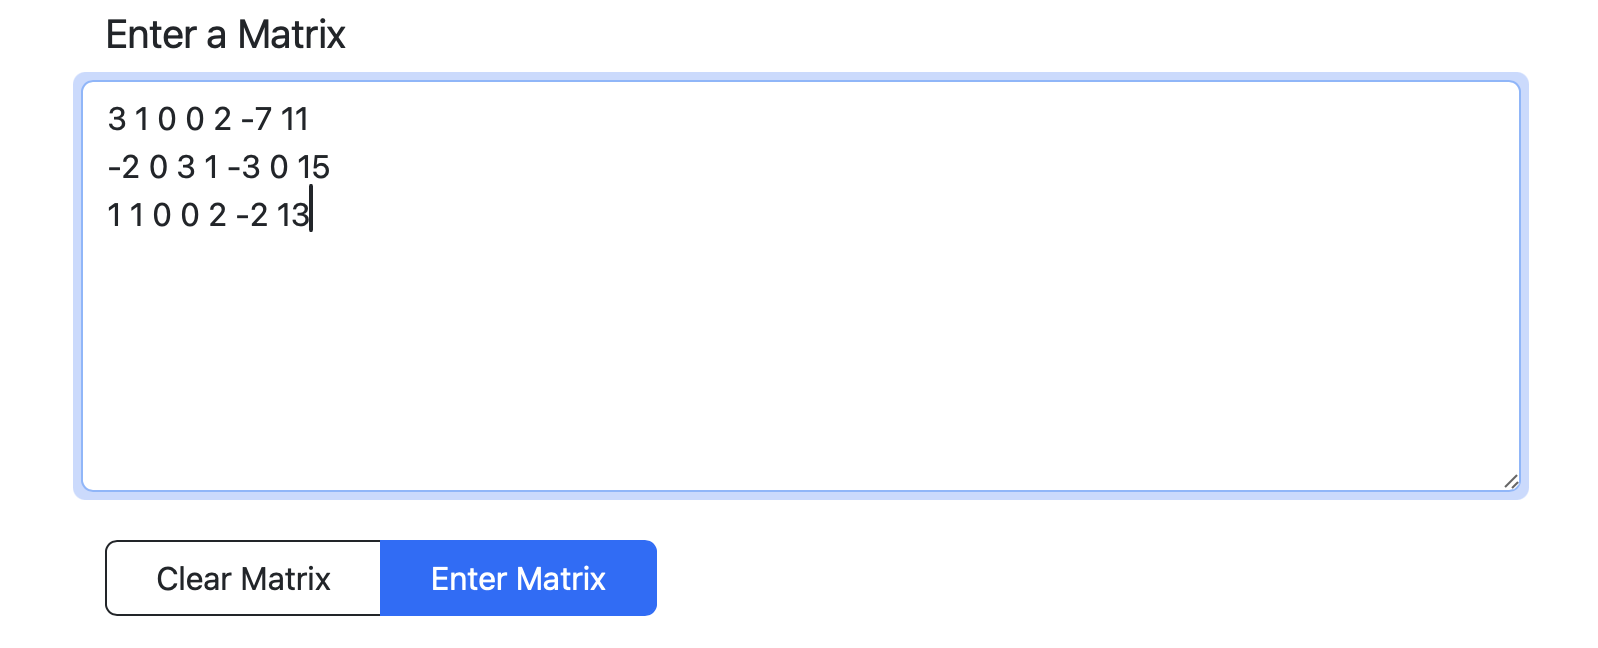
\includegraphics[width=\linewidth]{external/images/webcas01.png}
\end{image}%
\tcblower
\end{figureptx}%
and then click \emph{Enter Matrix} and you should see the matrix displayed in a mathematical form.%
\begin{note}{Note}{}{sect-webcas-rowop-5}%
Although the matrix above probably does not have the vertical line on the last column. This is a matrix decoration\textemdash{}it's purpose is to separate out the last column visually. To get this, click the gear icon in the top bar and the first option is \emph{Vertical Line Mode}. Select \emph{Before Last Column} then click \emph{Save Changes}.%
\par
You won't see them immediately, but if you click \emph{Restart} and then enter the matrix again, you should see the results that you expect.%
\end{note}
\begin{figureptx}{Figure}{The mathematical output of the matrix above put into WebCAS.}{fig-webcas2}{}%
\begin{image}{0.25}{0.5}{0.25}{}%
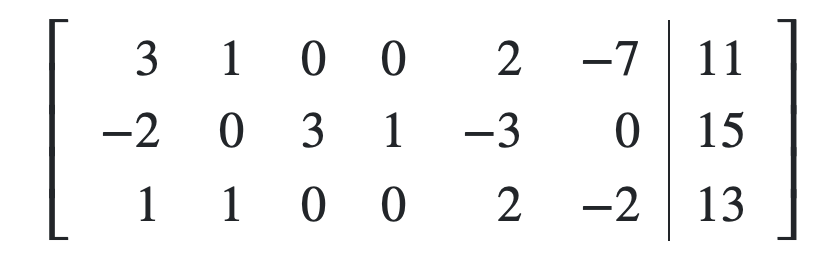
\includegraphics[width=\linewidth]{external/images/webcas2.png}
\end{image}%
\tcblower
\end{figureptx}%
To perform row operations in the Gaussian Eliminator, the following are supported%
\par
%
\begin{descriptionlist}
\begin{dlimedium}{Multiply Row by a Constant}{sect-webcas-rowop-8-1-1}%
If we want to multiply a row by a constant, like \(3R_2 \to R_2\), then enter \mono{3R2 -> R2}%
\end{dlimedium}%
\begin{dlimedium}{Multiply a Row by a Constant and add to another row}{sect-webcas-rowop-8-1-2}%
Mathematically, if you want to do \(R_1 + 3R_2 \to R_2\), in WebCAS, enter \mono{R1+3R2 -> R2}%
\end{dlimedium}%
\begin{dlimedium}{Linear Combination of Rows}{sect-webcas-rowop-8-1-3}%
A linear combination of rows is the above two operations above mushed together. This is often not an elementary row operation because for certain operations (like finding a determinant), one needs to be careful. However, this is a nice convenient operation for matrix pivots.%
\par
If you want to do \(-2R_1 + 3R_2 \to R_2\), then enter \mono{-2R1+3R2 -> R2}%
\end{dlimedium}%
\begin{dlimedium}{Row swaps}{sect-webcas-rowop-8-1-4}%
The row swap \(R_1 \leftrightarrow R_2\) can be done with \mono{R1 <-> R2}.%
\end{dlimedium}%
\end{descriptionlist}
%
\par
For the operations except the Row Swap, if you leave off the \mono{ -> R2} or an row, it will use the previous row as the row to insert. This way, complicated row operations can be done.%
\par
Returning to the matrix above from \hyperref[ex-lin-sys2]{Example~{\xreffont\ref{ex-lin-sys2}}}, we wanted to perform a matrix pivot about row 1, column 1. This was done with the two operations \(-2R_1 - 3R_2 \to R_2, R_1 -3R_3 \to R_3\) and in the Gaussian Eliminator, you can add both operations in the same box with \mono{-2R1-3R2->R2, R1-3R3->R3}. (Or drop the arrow and last row). Hitting the \emph{Enter} button (or the \emph{enter} key on your keyboard), you should see:%
\begin{figureptx}{Figure}{Row operations on the above matrix performed in WebCAS.  This is a matrix pivot about row 1, column 1 and the image is the result of the two operations.}{fig-webcas3}{}%
\begin{image}{0.05}{0.9}{0.05}{}%
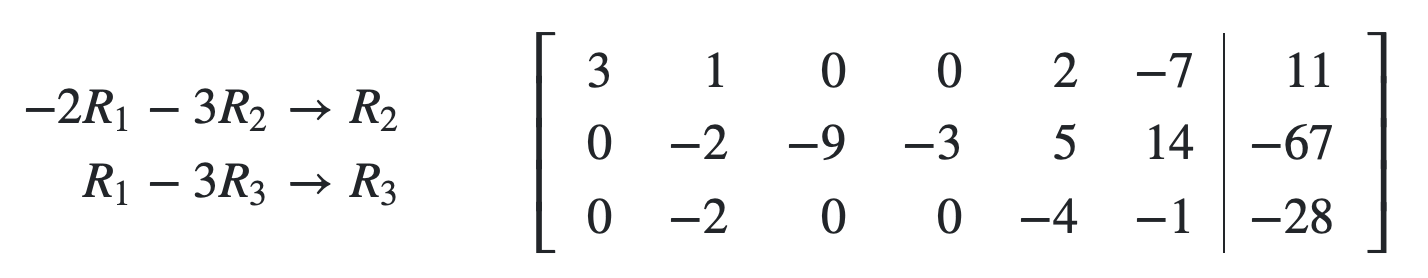
\includegraphics[width=\linewidth]{external/images/webcas3.png}
\end{image}%
\tcblower
\end{figureptx}%
\begin{note}{Note}{}{sect-webcas-rowop-12}%
Recall that on a matrix pivot the goal is to zero out the column that you are pivoting about (and we will want to get a positive number on the pivot element). Therefore, it should be clear that the pivot was done correctly. If not, there is an \emph{Undo} button which will bring back the previous matrix and reinserts the row operation. Edits can be done and re-entered.%
\par
From my experience over many years, this is the students' favorite feature of this tool.%
\end{note}
Continuing to do a matrix pivot on row 2, column 3, we do the following operation:%
\begin{figureptx}{Figure}{Row operations on the above matrix performed in WebCAS.  This is a matrix pivot about row 2, column 3 and the image is the result of the two operations.}{fig-webcas4}{}%
\begin{image}{0.05}{0.9}{0.05}{}%
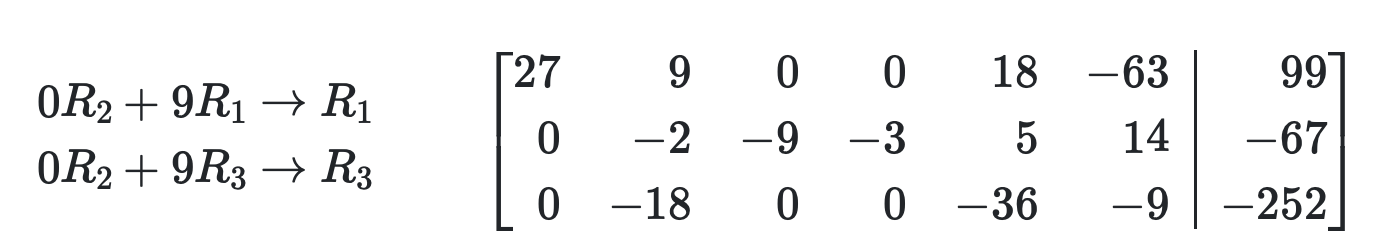
\includegraphics[width=\linewidth]{external/images/webcas04.png}
\end{image}%
\tcblower
\end{figureptx}%
Note that as we described in \hyperref[ex-lin-sys2]{Example~{\xreffont\ref{ex-lin-sys2}}}, this operation wasn't quite needed (the second row already is solved for \(x_3\)).  However, we did it to fit in with the standard pivot operations.%
\par
To finish the pivot, we need to negative the second row and then multiply the other two rows by \(1/3\), where \(3\) is used as the pivot value of the previous step.%
\begin{figureptx}{Figure}{Continued work on the previous pivot.  The second row is negated to ensure that the pivot element is positive.  Then the other two rows are multiplied by \(1/3\) to keep all previous pivots with the same value.}{fig-webcas5}{}%
\begin{image}{0.05}{0.9}{0.05}{}%
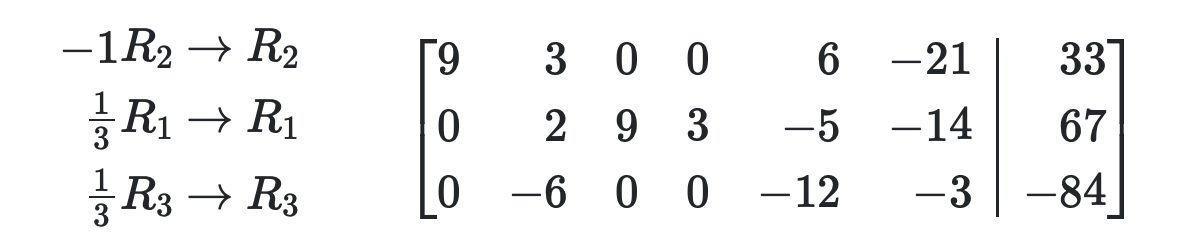
\includegraphics[width=\linewidth]{external/images/webcas05.png}
\end{image}%
\tcblower
\end{figureptx}%
The fraction operations are put in like \mono{1/3R1, 1/3R3} and a nice feature of WebCAS is that it uses fractions under the hood and doesn't do a floating-point divide that most languages might do with a \mono{1/3}.%
\par
The last pivot that we wanted to do is row 3, column 6. This can be done with%
\begin{figureptx}{Figure}{Row operations on the above matrix performed in WebCAS.  This is a matrix pivot about row 3, column 6 and the image is the result of the two operations.}{fig-webcas6}{}%
\begin{image}{0.05}{0.9}{0.05}{}%
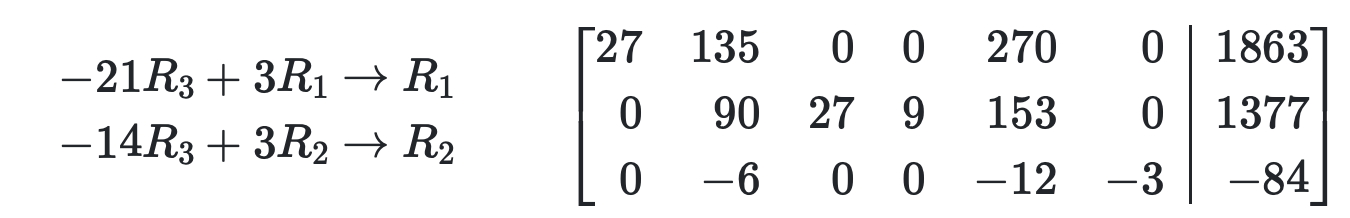
\includegraphics[width=\linewidth]{external/images/webcas06.png}
\end{image}%
\tcblower
\end{figureptx}%
and then we'll do the cleanup with%
\begin{figureptx}{Figure}{}{fig-webcas7}{}%
\begin{image}{0.05}{0.9}{0.05}{}%
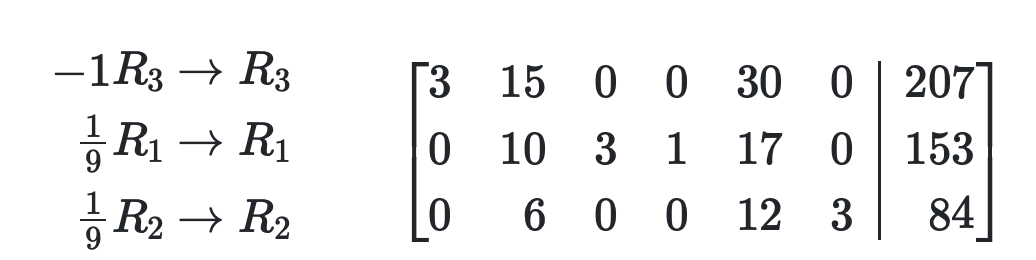
\includegraphics[width=\linewidth]{external/images/webcas07.png}
\end{image}%
\tcblower
\end{figureptx}%
and this is the same matrix that we got in \hyperref[ex-lin-sys2]{Example~{\xreffont\ref{ex-lin-sys2}}} and we could then right now the linear system and the solution as we did in that example.%
\end{subsectionptx}
%
%
\typeout{************************************************}
\typeout{Subsection 1.4.2 Matrix Pivots in WebCAS}
\typeout{************************************************}
%
\begin{subsectionptx}{Subsection}{Matrix Pivots in WebCAS}{}{Matrix Pivots in WebCAS}{}{}{sect-webcas-pivot}
You should clearly notice that using WebCAS to perform the row operations were quite nice in that it eliminates arithmetic errors. However, it still takes a number of steps that can be automated. In this section we will use the \mono{piv} command in WebCAS to further simplify these steps.%
\par
Let's return to \hyperref[ex-lin-sys2]{Example~{\xreffont\ref{ex-lin-sys2}}} and if you still have that matrix in the Gaussian Eliminator, then you can click \emph{Restart} and then reenter the matrix.\footnote{\begin{image}{0}{1}{0}{}%

\includegraphics[width=\linewidth]{external/images/matrix-movie.png}
\end{image}%
\label{sect-webcas-pivot-3-3}} Now at this step if we want to do a matrix pivot about row 1, column 1, then enter \mono{piv(1,1)}, and you should get:%
\begin{figureptx}{Figure}{Pivoting the original matrix about row 1 column 1.}{fig-webcas8}{}%
\begin{image}{0.125}{0.75}{0.125}{}%
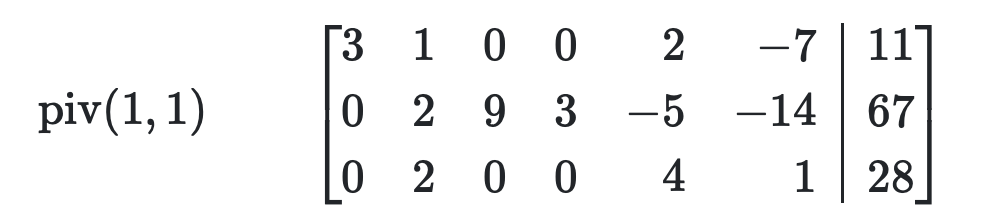
\includegraphics[width=\linewidth]{external/images/webcas08.png}
\end{image}%
\tcblower
\end{figureptx}%
And note that this differs from that of \hyperref[fig-webcas3]{Figure~{\xreffont\ref{fig-webcas3}}} in that the last two rows differ by a multiple of \(-1\). One can get from one to the other by row multiplications. The next pivot was about row 2, column 3, so entering \mono{piv(2,3)} results in%
\begin{figureptx}{Figure}{Pivoting the original matrix about row 2 column 3.}{fig-webcas9}{}%
\begin{image}{0.125}{0.75}{0.125}{}%
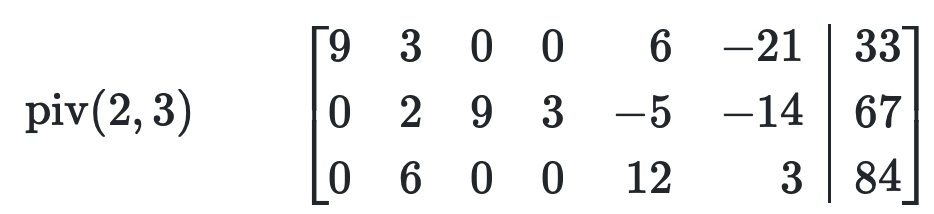
\includegraphics[width=\linewidth]{external/images/webcas09.png}
\end{image}%
\tcblower
\end{figureptx}%
and again this only differs by a sign in the last row in \hyperref[fig-webcas5]{Figure~{\xreffont\ref{fig-webcas5}}}. Lastly, we performed a pivot about row 3, column 6, so \mono{piv(3,6)} results in%
\begin{figureptx}{Figure}{Pivoting the original matrix about row 3 column 6.}{fig-webcas10}{}%
\begin{image}{0.125}{0.75}{0.125}{}%
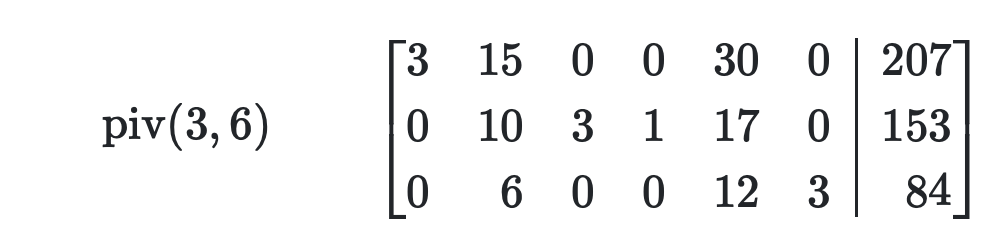
\includegraphics[width=\linewidth]{external/images/webcas10.png}
\end{image}%
\tcblower
\end{figureptx}%
and this is now equivalent to the matrix in \hyperref[fig-webcas7]{Figure~{\xreffont\ref{fig-webcas7}}}.  Using this fraction-free pivot method, or the \mono{piv} command in WebCAS will keep the matrix in integers and the pivot elements equal (and positive).  As we will see, using this and a related form of the pivot will simplify many operations used in later chapters.%
\end{subsectionptx}
%
%
\typeout{************************************************}
\typeout{Subsection 1.4.3 Click to Pivot in WebCAS}
\typeout{************************************************}
%
\begin{subsectionptx}{Subsection}{Click to Pivot in WebCAS}{}{Click to Pivot in WebCAS}{}{}{sect-click-to-pivot}
Another feature of WebCAS is \emph{Click To Pivot}.  When selected, this allows the user to click on an element in the matrix and perform the click.  Once enabled, you can simply click on any entry in the matrix to perform a pivot about that element. This feature streamlines the process, especially for larger matrices, by reducing the need to manually enter pivot commands. After clicking, the matrix will update automatically to reflect the pivot operation. This will help as the size of the matrix increases.%
\par
First, to use this in WebCAS, return to the settings (with the Gear icon) on the top bar, and enable the \emph{Click To Pivot} option then save the changes.%
\par
After this is set and a matrix is entered, there will be a Checkbox at the top.  Selecting the  \emph{Click to Pivot} option puts this in a click mode.%
\par
Enter a matrix in the standard way.  Then you can click on the number that you wish to pivot upon.%
\end{subsectionptx}
\end{sectionptx}
\end{chapterptx}
%
%
\typeout{************************************************}
\typeout{Chapter 2 Developing Linear Models}
\typeout{************************************************}
%
\begin{chapterptx}{Chapter}{Developing Linear Models}{}{Developing Linear Models}{}{}{ch-linear-models}
\renewcommand*{\chaptername}{Chapter}
\begin{introduction}{}%
Linear models arise from many different fields including business, manufacturing as well as the sciences. This chapter shows many applied problems and how they can be created mathematically into a category called linear optimization problems. For problems of only two variables it relatively straightforward to graph the constraints and make a geometric argument about where the optimal value is.%
\end{introduction}%
%
%
\typeout{************************************************}
\typeout{Section 2.1 Introduction to Linear Optimization}
\typeout{************************************************}
%
\begin{sectionptx}{Section}{Introduction to Linear Optimization}{}{Introduction to Linear Optimization}{}{}{sect-linear-models}
\begin{objectives}{Objectives}{sect-linear-models-2}
%
\begin{itemize}[label=\textbullet]
\item{}Provide examples of linear optimization problems.%
\item{}Writing down an applied problem as a mathematical linear optimization problem.%
\end{itemize}
\end{objectives}
\begin{introduction}{}%
This section goes into a number of applied problems that have linear constraints and a linear objective function. Consider the following:%
\begin{problem}{Problem}{The toy car problem.}{prob-toymaker}%
Luis is a toymaker who builds toy cars with wood. His most popular toys are a car, an SUV and a truck. The car is made with 6 units of pine, 3 units of birch and take a total of 45 minutes to make. The SUV is made with 5 units of pine, 6 units of birch and takes a total of 75 minutes to make. The truck takes 4 units of pine, 7 units of birch and takes a total of 90 minutes to make. For each car he makes \textdollar{}10 in profit, for each SUV is \textdollar{}15 in profit and for each truck is \textdollar{}12 in profit.%
\par
Luis has 183 units of pine, 204 units of birch. For the week, he has a total of 2655 minutes of time the shop can spend building toys. How many of each toy should he make to maximize his profit?%
\end{problem}
Example of Linear Optimization Problems (LOPs) occur in many fields. This section introduces a few more examples.%
\begin{problem}{Problem}{Shipping Coffee Problem.}{prob-coffee}%
A coffee supplier has warehouses in Seattle and San José. The coffee supplier receives orders from coffee retailers in Salt Lake City and Reno.%
\par
The retailer in Salt Lake City needs 400 pounds of coffee and the the retailer in Reno needs 350 pounds of coffee. The Seattle warehouse has 700 pounds available and the San José warehouse has 500 pounds available.%
\par
The cost of shipping from Seattle to Salt Lake City is \textdollar{}2.50 per pound, from Seattle to Reno \textdollar{}3 per pound, from San José to Salt Lake is \textdollar{}4 per pound and from San José to Reno is \textdollar{}2 per pound.%
\par
Find the number of pounds to be shipped from each warehouse to each retailer to minimize the cost.%
\end{problem}
\begin{problem}{Problem}{Scheduling Librarians.}{sect-linear-models-3-5}%
The FSU library needs to make sure that there is at least one reference librarian on duty during open hours. If there are 3 reference librarians, how do you schedule them to work such that a) each one works at least 30 hours per week. b) No one work longer than 10 hours in a given day. How would you schedule them such that the total number of hours worked by all reference librarians is minimized.%
\end{problem}
\begin{problem}{Problem}{A Diet Problem.}{prob-diet}%
Consider the problem: Gary goes on a diet eating only a salad, turkey sandwich or a bagel with cream cheese for a week. (Yes. It’s the worst!). The following table shows important information for each%
\begin{center}%
{\tabularfont%
\begin{tabular}{lllll}
&calories&protein&carbs&fat\tabularnewline\hrulemedium
salad&600&5&7&4\tabularnewline[0pt]
sandwich&750&18&10&8\tabularnewline[0pt]
bagel&500&10&24&12
\end{tabular}
}%
\end{center}%
Gary is trying to minimize the total calories ensuring that he eats at least 54 grams of protein, 45 grams of fat and 60 grams of carbs. Write down the objective function and the set of linear constraints?%
\end{problem}
\begin{problem}{Problem}{Blending Problem.}{sect-linear-models-3-7}%
\emph{Becky’s Bakery} has the following amounts of ingredients on hand: 32 cups flour, 2 dozen eggs and 20 cups of sugar. They would like to make some number of batches of Chocolate Chip Cookies, Brownies and Sugar Cookies. The recipes for these call for the following amounts of flour, eggs and sugar:%
\begin{center}%
{\tabularfont%
\begin{tabular}{llll}
Recipe&Flour&Eggs&Sugar\tabularnewline\hrulemedium
\tabularnewline[0pt]
Choc. Chip Cookies&3&2&1\tabularnewline[0pt]
Brownies&2&1&2\tabularnewline[0pt]
Sugar Cookies&1&2&2
\end{tabular}
}%
\end{center}%
If the profit made for each recipe is 20, 24, and 16 dollars respectively, find the number of batches of each baked good that the bakery should make to maximize the profit.%
\end{problem}
\begin{problem}{Problem}{Allocation Problem.}{sect-linear-models-3-8}%
Jane has four courses this given semester. Let's call them Mathematics (M), History (H), Writing (W) and Psychology (Psy). We want to determine a number of constraints on the amount of studying she does in these classes.%
\par
%
\begin{enumerate}
\item{}The total number of hours for studying is 360.%
\item{}Jane is on a scholarship and needs to keep a 3.0.%
\item{}Jane needs to pass every class to stay on the scholarship.%
\item{}From past experience, the following table lists the amount of time Jane needs to earn 1 grade point in each course:%
\begin{center}%
{\tabularfont%
\begin{tabular}{ll}
Course&hour\slash{}grade point\tabularnewline\hrulemedium
Mathematics&30\tabularnewline[0pt]
Psychology&20\tabularnewline[0pt]
History&25\tabularnewline[0pt]
Writing&20
\end{tabular}
}%
\end{center}%
\end{enumerate}
%
\par
What is the minimum number of hours that Jane should study in each class?%
\end{problem}
\begin{problem}{Problem}{Urban Farming Project.}{prob-urban-farm}%
A non-profit organization, \emph{GreenHarvest}, aims to establish a sustainable urban farm within a limited city space.\footnotemark{} They want to maximize their total profit from selling produce to local restaurants and farmers' markets while adhering to various constraints. They have identified four key crops to cultivate:%
\par
%
\begin{enumerate}
\item{}Heirloom Tomatoes (T): High-profit, but require significant space and water.%
\item{}Organic Lettuce (L): Moderate profit, quick growing, but sensitive to sun exposure.%
\item{}Specialty Herbs (H): Low profit per plant, but very space-efficient and high demand.%
\item{}Root Vegetables (R): Moderate profit, require deep soil beds and longer growth cycles.%
\end{enumerate}
%
\par
The project has 50 growing beds for all crops. Due to city regulations and sustainable practices, there's a limit on daily water consumption. Each crop type has different water requirements per bed. The total water usage cannot exceed 1500 liters per day.%
\par
%
\begin{itemize}[label=\textbullet]
\item{}Heirloom Tomatoes: 40 liters\slash{}bed%
\item{}Organic Lettuce: 25 liters\slash{}bed%
\item{}Specialty Herbs: 15 liters\slash{}bed%
\item{}Root Vegetables: 30 liters\slash{}bed%
\end{itemize}
%
\par
To meet the demand from local restaurants that rely heavily on fresh herbs, GreenHarvest wants to ensure at least 5 beds are dedicated to Specialty Herbs.%
\par
To maintain crop diversity and manage pest control effectively, the number of Heirloom Tomato beds should be no more than twice the number of Organic Lettuce beds.%
\par
Profit per bed (estimated per growing season):%
\par
%
\begin{enumerate}
\item{}Heirloom Tomatoes: \textdollar{}300%
\item{}Organic Lettuce: \textdollar{}180%
\item{}Specialty Herbs: \textdollar{}100%
\item{}Root Vegetables: \textdollar{}220%
\end{enumerate}
%
\par
The goal of this problem is to determine the number of beds to devote to each of the different types of crops in order to maximize the profit.%
\end{problem}
\footnotetext[1]{This problem was created in part using Google Gemini.\label{prob-urban-farm-2-2}}%
\end{introduction}%
%
%
\typeout{************************************************}
\typeout{Subsection 2.1.1 Creating Linear Models}
\typeout{************************************************}
%
\begin{subsectionptx}{Subsection}{Creating Linear Models}{}{Creating Linear Models}{}{}{sect-create-linear-model}
We have seen a number of problems in this chapter that will fit into a linear model. Let's look at \hyperref[prob-toymaker]{Problem~{\xreffont\ref{prob-toymaker}}} as a example of how to approach creating a linear model. We'll write the common steps and fill in those steps for this problem.%
\par
%
\begin{enumerate}
\item{}What are the variables? Clearly list each one or perhaps if they are indexed, write down what each indexed variable represents.%
\par
\alert{Solution:} There are 3 types of toys for this problem:%
\par
%
\begin{align*}
x_1 \amp = \text{number of cars to be produced},\\
x_2 \amp = \text{number of SUVs to be produced},\\
x_3 \amp = \text{number of trucks to be produced}.
\end{align*}
%
\item{}What is the objective?   Is it to be minimized or maximized.%
\par
\alert{Solution:} In this case, the profit is to be \emph{maximized} and can be written%
\par
%
\begin{equation*}
z = 10 x_1 + 15 x_2 + 12 x_3.
\end{equation*}
%
\item{}What are the constraints?  Note: one way to think about this is the case of something being maximized, why can't the objective be increased without bound.%
\par
\alert{Solution:} The profit cannot be increased with bound because there is a limit on the amount of wood and labor that can be used.  For each of these, we build a constraint.%
\par
%
\begin{itemize}[label=\textbullet]
\item{}For the amount of pine: \(6x_1 + 5x_2 + 4x_3 \leq 183.\)%
\item{}For the amount of birch: \(3x_1 + 6x_2 + 7x_3 \leq 204.\)%
\item{}For the amount of labor: \(45x_1 + 75x_2 + 90x_3 \leq 2655.\)%
\end{itemize}
%
\item{}Check if the nonnegative constraints on the variables are needed assumptions.%
\par
\alert{Solution:} Yes.  Since the variables represent the numbers of things (in this case toys) to make, the nonnegative assumptions on each variable makes sense.%
\par
%
\begin{equation*}
x_1, x_2, x_3 \geq 0
\end{equation*}
%
\item{}Check if either integer or binary constraints are reasonable.%
\par
\alert{Solution:} Since the variables are numbers of toys to make, they must be integers,\footnote{There are a few different ways to denote the set of nonnegative integers, however, in this text, we will use \(\mathbb{N}_0\) to represent \(\{0,1,2,3, \ldots \}\).\label{sect-create-linear-model-3-1-5-2-2}} but not binary.%
\par
%
\begin{equation*}
x_1, x_2, x_3 \in \mathbb{N}_0
\end{equation*}
%
\end{enumerate}
%
\par
The next problem shows how to attack another linear problem.%
\begin{problem}{Problem}{}{prob-coffee-setup}%
Use the steps above to write the LOP for \hyperref[prob-coffee]{Problem~{\xreffont\ref{prob-coffee}}}.%
\par\smallskip%
\noindent\textbf{\blocktitlefont Solution}.\hypertarget{prob-coffee-setup-2}{}\quad{}%
\begin{enumerate}
\item{}What are the variables?%
\par
\alert{Solution:} In this case, first note that we need to know the amount of coffee shipped between warehouses and retail outlets. The following graph is helpful for this:%
\begin{figureptx}{Figure}{}{fig-coffee}{}%
\begin{image}{0.2}{0.6}{0.2}{}%
\resizebox{\linewidth}{!}{%
\begin{tikzpicture}
  \draw[->] (1,5) -- (5,0) node[pos=0.25, above right] {$x_1$};
  \draw[->] (0.5,5) -- (0.5,0) node[midway, left] {$x_2$};
  \draw[->] (5,5) -- (1,0) node[pos=0.25, above left] {$x_3$};
  \draw[->] (5.5,5) -- (5.5,0) node[midway, right] {$x_4$};
  \draw (0.5,5) node[above] {Seattle};
  \draw (5,5) node[above] {San Jos\'e};
  \draw (0.5,0) node[below] {Salt Lake City};
  \draw (5.5,0) node [below] {Reno};
\end{tikzpicture}%
}%
\end{image}%
\tcblower
\end{figureptx}%
Specifically we have the following:%
\par
%
\begin{align*}
x_1 \amp = \text{number of pounds of coffee to ship from Seattle to Reno},\\
x_2 \amp = \text{number of pounds of coffee to ship from Seattle to Salt Lake City},\\
x_3 \amp = \text{number of pounds of coffee to ship from San José  to Reno},\\
x_4 \amp = \text{number of pounds of coffee to ship from San José to Salt Lake. City}
\end{align*}
%
\item{}\emph{What is the objective?}%
\par
The objective is the total cost and it is to be minimized or%
\par
%
\begin{equation*}
z = 3 x_1 + 2.50 x_2 + 4 x_3 + 2 x_4.
\end{equation*}
%
\item{}\emph{What are the constraints?}%
\par
The variables are going to be the total amount of coffee to be shipped from the two warehouses to the two retail locations. If we look first at the amount of coffee that the Salt Lake City and Reno locations need then we need to ship at least this amount or%
\par
%
\begin{align*}
x_2 + x_3 \amp \geq 400, \\
x_1 + x_4 \amp \geq 350.
\end{align*}
%
\par
Since the warehouses have a limited supply, they can only ship what they have so there are two additional constraints, one for each warehouse%
\par
%
\begin{align*}
x_1 + x_2 \amp \leq 700,\\
x_3 + x_4 \amp \leq 500.
\end{align*}
%
\item{}Check if the nonnegative constraints on the variables are needed assumptions.%
\par
\alert{Solution:} Each amount of coffee shipped should be nonnegative, so \(x_1, x_2, x_3, x_4 \geq 0\).%
\item{}\emph{Check if either integer or binary constraint are needed.}%
\par
In this case, because coffee does not need to be shipped in integer amounts of pounds, this is not needed.%
\end{enumerate}
%
\par
We can combine all of these into the following LOP:%
\par
%
\begin{equation*}
\begin{aligned} \text{Minimize} \amp \amp  z = 2.5 x_1 + 3 x_2 + 4 x_3 + 2 x_4,\amp \\ \text{subject to} \amp \amp x_2 + x_3 \amp \geq 400.\\ \amp \amp x_1 + x_4 \amp \geq 350,\\ \amp \amp x_1 + x_2 \amp \leq 700,\\ \amp \amp x_3 + x_4 \amp \leq 500,\\ \text{and}\amp \amp x_1, x_2, x_3, x_4 \amp \geq 0.
\end{aligned}
\end{equation*}
%
\end{problem}
\end{subsectionptx}
%
%
\typeout{************************************************}
\typeout{Subsection 2.1.2 Non-Obvious Linear Optimization Problems}
\typeout{************************************************}
%
\begin{subsectionptx}{Subsection}{Non-Obvious Linear Optimization Problems}{}{Non-Obvious Linear Optimization Problems}{}{}{sect-other-problems}
\begin{introduction}{}%
Perhaps as you have read through the problems at the top of this section and then the mathematical formulation of each in \hyperref[sect-create-linear-model]{Subsection~{\xreffont\ref{sect-create-linear-model}}} and notice that there are some similarities between the problems. Each clearly has an objective that is to optimized and has a number of constraints. However, there are other problems that with some creativity can be written as an LOP. Consider the following:%
\begin{problem}{Problem}{\(n\)-queens problem.}{prob-n-queens}%
A chessboard is a grid of spaces in which pieces move around the board according to various rules. A queen is a piece that can move left, right, up, down or diagonal any number of squares. \hyperref[fig-chessboard-queen]{Figure~{\xreffont\ref{fig-chessboard-queen}}} shows the standard 8 by 8 chessboard and one queen.%
\par
The \(n\)-queens problem asks if \(n\) queens can appear on an \(n\) by \(n\) chessboard, so that no queen can attacker another queen.%
\end{problem}
\begin{figureptx}{Figure}{An 8 by 8 chessboard with a queen on a square.  The arrows indicate the other squares that can attack with this piece.}{fig-chessboard-queen}{}%
\begin{image}{0.25}{0.5}{0.25}{}%
\resizebox{\linewidth}{!}{%
\begin{tikzpicture}[scale=0.5]
  \draw[lightgray] (0,0) grid (8,8);
  \draw (2.5, 1.5) node {\symqueen};
  \draw[thick, ->] (2.8, 1.5) -- (7.5,1.5);
  \draw[thick, ->] (2.1, 1.5) -- (0.5,1.5);
  \draw[thick, ->] (2.1, 1.1) -- (1.5, 0.5);
  \draw[thick, ->] (2.5, 1.1) -- (2.5, 0.5);
  \draw[thick, ->] (2.9, 1.1) -- (3.5, 0.5);
  \draw[thick, ->] (2.1, 1.9) -- (0.5, 3.5);
  \draw[thick, ->] (2.5, 1.9) -- (2.5, 7.5);
  \draw[thick, ->] (2.9, 1.9) -- (7.5, 6.5);
\end{tikzpicture}%
}%
\end{image}%
\tcblower
\end{figureptx}%
It's not clear what the objective function is for this problem (although there is one). The constraints for the problem might be the constraints on a queen. Also, what are the variables?  We'll see how to approach this later.%
\begin{problem}{Problem}{Room Scheduling.}{sect-other-problems-2-5}%
The registrar at State University needs to schedule rooms for a set of classes in a time block. For simplification, the classes will be A, B, C, ..., H and they will be put in rooms 1,2,3, ..., 8. Not every class can be scheduled in every room. Some classes need to be in a computer class, some classes need to be on the first floor of the building, some faculty prefer whiteboards, some faculty prefer to use a project. Here's all of these constraints:%
\par
%
\begin{itemize}[label=\textbullet]
\item{}Classes A, B and C need to be scheduled in a computer lab (rooms 1, 4, 6, 8).%
\item{}Classes D and E need to be on the first floor the building (rooms 1, 2, 3).%
\item{}Classes B, E, F, G, H need a whiteboard and cannot be in rooms 1, 2 or 7.%
\item{}Classes C, D, F and H need a projector and cannot be in room 2, 5, or 8.%
\end{itemize}
%
\par
What is a reasonable scheduling of the rooms if possible?%
\end{problem}
This problem seems to have similarities with the previous problem, and similar questions arise. What are the variables for the problem?  There are clearly some constraints in that certain classes need to be in a some rooms, but not others. It's unclear what the objective is.%
\begin{problem}{Problem}{Mars Rover.}{prob-mars-rover}%
You are the lead mission planner for NASA's new Mars rover, ``Curiosity II.'' The rocket launching the rover has a strict weight limit for its scientific payload. Exceeding this limit is not an option. A team of scientists has reviewed all possible instruments and assigned each a ``scientific value'' score based on the mission's objectives (like finding signs of past life or analyzing atmospheric composition). Your job is to select the combination of instruments that will maximize the total scientific value of the mission without exceeding the weight limit. \footnotemark{}%
\begin{tableptx}{Table}{\textbf{Mars Rover Instrument Options}}{table-knapsack-rover}{}%
\centering%
{\tabularfont%
\begin{tabular}{lll}
{\bfseries{}Instrument Name}&\multicolumn{1}{c}{{\bfseries{}Weight (kg)}}&\multicolumn{1}{c}{{\bfseries{}Scientific Value Score}}\tabularnewline\hrulemedium
Alpha Particle X-ray Spectrometer&\multicolumn{1}{c}{35}&\multicolumn{1}{c}{30}\tabularnewline[0pt]
High-Resolution Panoramic Camera&\multicolumn{1}{c}{30}&\multicolumn{1}{c}{25}\tabularnewline[0pt]
Subsurface Drilling Unit&\multicolumn{1}{c}{60}&\multicolumn{1}{c}{55}\tabularnewline[0pt]
Weather \& Radiation Monitor&\multicolumn{1}{c}{45}&\multicolumn{1}{c}{35}\tabularnewline[0pt]
Laser-Induced Breakdown Spectrometer&\multicolumn{1}{c}{40}&\multicolumn{1}{c}{40}\tabularnewline[0pt]
Robotic Scoop \& Soil Analyzer&\multicolumn{1}{c}{55}&\multicolumn{1}{c}{50}
\end{tabular}
}%
\end{tableptx}%
\end{problem}
\footnotetext[3]{This was generated with help from Gemini AI.\label{prob-mars-rover-2-3}}%
This problem falls into a class of problems called knapsack problems. The idea is that you have a knapsack (backpack) with limited capacity and you want to include as much as possible, whether that is volume, weight or some other measure (like scientific value).%
\begin{problem}{Problem}{The Mailbox Problem.}{prob-mailbox}%
Consider a city that is 4 blocks by 6 blocks in a grid as shown below%
\begin{figureptx}{Figure}{}{fig-gridburg}{}%
\begin{image}{0.125}{0.75}{0.125}{}%
\resizebox{\linewidth}{!}{%
\begin{tikzpicture}
\draw (0,0) grid (6,4);
\end{tikzpicture}%
}%
\end{image}%
\tcblower
\end{figureptx}%
The postal chief wants to arrange mailboxes such that anywhere in the city, one does not need to walk any more than one block to reach a mailbox.  Where should the mailboxes be placed to minimize the number of mailboxes.\footnotemark{}%
\end{problem}
\footnotetext[4]{This problem is a nod to Glenn Hurlbert, whose book \emph{Linear Optimization: a Handbook} motivated this work.  The book had a number of problems in \emph{Gridburg} a town on a grid like above.\label{prob-mailbox-2-3-1}}%
\end{introduction}%
%
%
\typeout{************************************************}
\typeout{Subsubsection 2.1.2.1 LOP Formulation of \(n\)-queens Problem}
\typeout{************************************************}
%
\begin{subsubsectionptx}{Subsubsection}{LOP Formulation of \(n\)-queens Problem}{}{LOP Formulation of \(n\)-queens Problem}{}{}{prob-n-queens-form}
Perhaps looking at \hyperref[prob-n-queens]{Problem~{\xreffont\ref{prob-n-queens}}}, it would not seem like it is a linear optimization problem. You might think that there are constraints\textemdash{}no queen can attack another one, but what is the objective function?%
\par
First, to formulate the problem, we need to know the variables. A common situation is to place objects in a grid or other arrangement and then use a variable to denote whether or not to place the object at the grid point. In this case, we are going to use \(x_{i,j}\) to be a binary variable that is 1 if there is a queen at row \(i\) and column \(j\) and 0 otherwise.%
\par
The constraints will be that there is at most one queen in any row, column or diagonal of the chessboard. At most a single queen in any row or column can be written as%
\par
%
\begin{align}
\sum_{j=1}^n x_{i,j} \amp \leq 1 \qquad \text{for $i=1, 2, \ldots n$} \label{eq-queen-row}\\
\sum_{i=1}^n x_{i,j} \amp \leq 1 \qquad \text{for $j=1, 2, \ldots n$} \label{eq-queen-col}
\end{align}
%
\par
Note that in \hyperref[eq-queen-row]{({\xreffont\ref{eq-queen-row}})}, the sum is across row \(i\) and the inequality with \(\leq 1\) means that at most there is 1 queen in each row. Similarly in \hyperref[eq-queen-col]{({\xreffont\ref{eq-queen-col}})}, the sum in for a given column, so there is at most one queen in a column.%
\par
The diagonals are trickier. In the diagonal from the lower left to upper right then summing \(\sum_{i=1}^n x_{i,i}  \leq 1 \), but this is also true for every diagonal that parallels this one. The inequality for this is in the problem below.%
\par
There is also a diagonal from the upper left to lower right with the inequality \(\sum_{i=1}^n x_{i,n+1-i} \leq 1\), but also with every other diagonal parallel to these, which are listed below.%
\par
Finally, we will use the objective that the total number of queens on the board to be minimized. The total number can be calculated with%
\par
%
\begin{equation*}
z = \sum_{i=1}^n \sum_{j=1}^n x_{i,j}
\end{equation*}
%
\par
Here's a summary of the \(n\)-queens problems:%
\par
%
\begin{equation*}
\begin{aligned} \text{Minimize} \amp \amp z \amp = \sum_{i=1}^n \sum_{j=1}^n x_{i,j}, \\ \text{subject to} \amp \amp \sum_{i=1}^n x_{i,j} \amp \leq 1 \qquad \text{for $j=1, 2, \ldots n$} \\ \amp \amp \sum_{j=1}^n x_{i,j} \amp \leq 1 \qquad \text{for $i=1, 2, \ldots n$} \\ \amp \amp \sum_{i=1}^{n-k} x_{i,i+k} \amp \leq 1 \qquad \text{for $k=0, 1, \ldots n-1$} \\ \amp \amp \sum_{i=k-1}^{n-1} x_{i,i-k} \amp \leq 1 \qquad \text{for $k=1,2, \ldots n-1$} \\ \amp \amp \sum_{i=1}^{n-k} x_{i,n-k} \amp \leq 1 \qquad \text{for $k=0, 1, \ldots n-1$} \\ \amp \amp \sum_{i=k-1}^{n-1} x_{n-i,k} \amp \leq 1 \qquad \text{for $k=1,2, \ldots n-1$} \\ \text{and} \amp \amp x_{i,j} \amp \in \{0,1\} \qquad \text{for $i=1,\ldots, n, j = 1, \ldots n$} \end{aligned}
\end{equation*}
%
\par
The first inequality is the column sum for every \(j\), the second is the row sum for every \(i\). The third and fourth are the diagonals that run from bottom left to upper right on the chessboard and the fifth and sixth are the upper left to lower right.%
\end{subsubsectionptx}
\end{subsectionptx}
\end{sectionptx}
%
%
\typeout{************************************************}
\typeout{Section 2.2 Linear Optimization Problems}
\typeout{************************************************}
%
\begin{sectionptx}{Section}{Linear Optimization Problems}{}{Linear Optimization Problems}{}{}{sect-lops}
\begin{objectives}{Objectives}{sect-lops-2}
%
\begin{itemize}[label=\textbullet]
\item{}Definition of a Linear Optimization Problem and related problems.%
\item{}Definition of the Standard Form of an LOP%
\item{}How to put a minimum problem into standard form%
\item{}General Form of an LOP%
\end{itemize}
\end{objectives}
\begin{introduction}{}%
In the previous two sections of this chapter we have seen applied problems as well as feasible sets. In this section, we will summarize all of these and determine a method to put applied problems into a mathematical formulation.%
\end{introduction}%
%
%
\typeout{************************************************}
\typeout{Subsection 2.2.1 Definitions and Conventions}
\typeout{************************************************}
%
\begin{subsectionptx}{Subsection}{Definitions and Conventions}{}{Definitions and Conventions}{}{}{sect-def-lop}
\begin{definition}{Definition}{}{def-lop}%
A \terminology{Linear Optimization Problem}\footnotemark{} consists of%
\par
%
\begin{itemize}[label=\textbullet]
\item{}A linear objective function that is to be minimized or maximized.%
\item{}A set of linear inequalities.%
\item{}A set of nonnegative constraints on the variables.%
\end{itemize}
%
\par
In short, we will call such problems \terminology{LOPs} and if the variables are constrained to be integers, then such problems are \terminology{Integer Linear Optimization Problems} or \terminology{ILOPs} and if the variables are constrained to be binary, then the problems are \terminology{Binary Linear Optimization Problems} or \terminology{BLOPs} .%
\end{definition}
\footnotetext[1]{This is not the most general form of such a problem.  We will see a general linear optimization problem in \hyperref[ch-general-lops]{Chapter~{\xreffont\ref{ch-general-lops}}}.\label{def-lop-1-1-2}}%
Let's take a look at an purely mathematical example of an LOP.%
\begin{problem}{Problem}{}{prob-lop1}%
%
\begin{equation*}
\begin{aligned} \text{Maximize} \amp \amp z = x_1 + 3x_2, \amp \\ \text{subject to} \amp \amp 4x_1 + 3x_2 \amp \leq 120, \\ \amp \amp x_1 + 2x_2 \amp \leq 40, \\ \amp \amp x_2 \amp \leq 16, \\ \text{and} \amp \amp x_1, x_2 \amp \geq 0.
\end{aligned}
\end{equation*}
%
\end{problem}
A few conventions that we will use in this book:%
\par
%
\begin{itemize}[label=\textbullet]
\item{}This is a \emph{maximum} problem, so we will use the variable \(z\) for the objective and \(x_i\) for each of the variables.%
\item{}If instead we have a \emph{minimum} problem, then we will use \(w\) for the objective and \(y_i\) for the variables. We will see another problem like this later.%
\item{}The variables (either \(x_i\) or \(y_i\)) need to have the non-negative constraint that is the last line of the LOP in \hyperref[prob-lop1]{Problem~{\xreffont\ref{prob-lop1}}}.%
\end{itemize}
%
\begin{note}{Note}{}{sect-def-lop-7}%
Many LOPs naturally have the nonnegative constraint, because they arise from realistic problems in which variables cannot be negative. however, more abstract problems or mathematical problems may not have such constraints. We will learn in \hyperref[ch-general-lops]{Chapter~{\xreffont\ref{ch-general-lops}}} how to either take such problems and both add nonnegative constraints and then solve them without such constraints.%
\end{note}
An example of a minimum problem is the following.%
\begin{problem}{Problem}{}{prob-min-lop}%
%
\begin{equation*}
\begin{aligned} \text{Minimize} \amp \amp w = 4y_1 + 3y_2, \amp \\ \text{subject to} \amp \amp y_1 + y_2 \amp \geq 40, \\ \amp \amp 3y_1 + 2y_2 \amp \geq 95, \\ \amp \amp y_1 + 4 y_2 \amp \geq 55, \\ \text{and} \amp \amp y_1, y_2 \amp \geq 0.
\end{aligned}
\end{equation*}
%
\end{problem}
As you can see, we have use the variable \(w\) for the objective function and \(y_i\) for the variable. Another difference with \hyperref[prob-lop1]{Problem~{\xreffont\ref{prob-lop1}}} is that the first three constraints are of the form \(\geq\). Although this is not necessary, it is common. We will graph this feasible set in the next section and the characteristics of this set often are paired with a minimum problem.%
\end{subsectionptx}
%
%
\typeout{************************************************}
\typeout{Subsection 2.2.2 Standard Form}
\typeout{************************************************}
%
\begin{subsectionptx}{Subsection}{Standard Form}{}{Standard Form}{}{}{sect-std-form}
The LOP that we have been working on the past two section is in a special form that is needed for solving these problems using a technique we will develop in \hyperref[ch-simplex]{Chapter~{\xreffont\ref{ch-simplex}}}. We define it below and then explain how to get other problems into this form.%
\begin{definition}{Definition}{}{def-std-max-form}%
A Linear Optimization Problem is in \terminology{standard form} if the following are conditions are met:%
\begin{enumerate}
\item{}It is a maximum problem.%
\item{}All the constraints are of the form \(\leq b\), some constant.%
\item{}All variables are nonnegative.%
\end{enumerate}
%
\end{definition}
Not all LOPs are in standard form. Clearly \hyperref[prob-min-lop]{Problem~{\xreffont\ref{prob-min-lop}}} and many in \hyperref[sect-linear-models]{Section~{\xreffont\ref{sect-linear-models}}} as well. However, there is a systematic way to put such problems in standard form.%
\par
%
\begin{enumerate}
\item{}If the problem is a minimize problem in the form \(w = c_1 y_1 + c_2 y_2 + \cdots c_n y_n\), define \(z=-(c_1 y_1 + c_2 y_2 + \cdots + c_n y_n)\).%
\item{}Any inequality in the form \(a_1 x_1 + a_2 x_2 + \cdots + a_n x_n \geq b_n \) should be multiplied by \(-1\) to get%
\par
%
\begin{equation*}
-a_1 x_1 - a_2 x_2 - \cdots a_n x_n \leq -b_n
\end{equation*}
%
\item{}There are techniques to handle cases when the nonnegative constraint is not satisfied.  We will see how to handle these cases in \hyperref[ch-general-lops]{Chapter~{\xreffont\ref{ch-general-lops}}}.%
\end{enumerate}
%
\par
The following example shows how to put an LOP that is not in Standard Form into one that is.%
\begin{example}{Example}{}{sect-std-form-7}%
Put \hyperref[prob-min-lop]{Problem~{\xreffont\ref{prob-min-lop}}} in standard form.%
\par\smallskip%
\noindent\textbf{\blocktitlefont Solution}.\hypertarget{sect-std-form-7-2}{}\quad{}First, if the objective is a minimum problem, then we can make it a maximum problem by writing \(z=-w\). In this case, \(z=-3y_1-2y_2\).%
\par
Next, to get the inequalities in the proper form, multiply by \(-1\) and recall that changes a \(\geq\) to a \(\leq\). In this problems%
\par
%
\begin{align*}
-y_1 - y_2 \amp \leq -40,\\
-3y_1-2y_2 \amp \leq -95,\\
-y_1-4y_2 \amp \leq -55.
\end{align*}
%
\par
Therefore the problem in \emph{Standard Form} is%
\par
%
\begin{equation*}
\begin{aligned} \text{Maximize}\amp \amp z  = -3 y_1 - 2y_2,\amp \\ \text{subject to}\amp\amp -y_1 - y_2 \amp \leq -40, \\ \amp \amp-3y_1-2y_2 \amp \leq -95, \\ \amp \amp -y_1-4y_2 \amp \leq -55,\\ \text{and}\amp\amp y_1, y_2 \amp \geq 0.
\end{aligned}
\end{equation*}
%
\end{example}
\end{subsectionptx}
%
%
\typeout{************************************************}
\typeout{Subsection 2.2.3 General and Matrix Forms of an LOP}
\typeout{************************************************}
%
\begin{subsectionptx}{Subsection}{General and Matrix Forms of an LOP}{}{General and Matrix Forms of an LOP}{}{}{sect-lop-general}
In this section, we write the \terminology{General Form} of an Linear Optimization problem. Assume that there are \(n\) variables. If we have a maximum problem, we will use the variables \(x_i\) and a general constraint can be written%
\par
%
\begin{equation*}
\sum_{j=1}^n a_{i,j} x_j \leq b_i,
\end{equation*}
%
\par
where  \(i\) will be between 1 and \(m\). So in general a maximum problem can be written:%
\par
%
\begin{equation*}
\begin{aligned} \text{Maximize} \amp \amp  z = \sum_{j=1}^n c_j x_j  \amp \\ \text{subject to} \amp \amp \sum_{j=1}^n a_{i,j} x_j \leq b_i \amp \qquad \text{where $i=1,2,\ldots,n$}, \\ \text{and} \amp \amp  x_j \geq 0, \amp \qquad\text{where $j=1,2, \ldots,n$}. \end{aligned}
\end{equation*}
%
\par
These problems can be written in \terminology{Matrix Form} in the following way:%
\par
%
\begin{equation*}
\begin{aligned}
\text{Maximize} \amp \amp z = \boldsymbol{c}^{\intercal}\boldsymbol{x}, \amp \\
\text{subject to} \amp \amp A \boldsymbol{x} \leq \boldsymbol{b}, \\
\text{and} \amp \amp \boldsymbol{x} \geq \boldsymbol{0}.
\end{aligned}
\end{equation*}
%
\par
where the inequalities must hold for each element of the vector.%
\end{subsectionptx}
\end{sectionptx}
%
%
\typeout{************************************************}
\typeout{Section 2.3 Geometry of Feasible Sets}
\typeout{************************************************}
%
\begin{sectionptx}{Section}{Geometry of Feasible Sets}{}{Geometry of Feasible Sets}{}{}{sect-geometry}
\begin{objectives}{Objectives}{sect-geometry-2}
%
\begin{itemize}[label=\textbullet]
\item{}The definition of a \terminology{feasible set}.%
\item{}How to graph a feasible set in the \(xy\)-plane.%
\item{}The structure of a feasible set and how it helps solve LOPs%
\item{}The convexity of feasible sets.%
\end{itemize}
\end{objectives}
\begin{introduction}{}%
In the \hyperref[sect-linear-models]{Section~{\xreffont\ref{sect-linear-models}}}, we saw many different type of problems that fall into linear optimization. Many of these problems had a lot of variables and as we will see in this course is it easy to get tens or hundreds of variables.%
\begin{definition}{Definition}{}{def-feasible-set}%
Consider a set of linear inequalities that arise from an Linear Optimization Problem in standard form:%
\par
%
\begin{align*}
a_{11} x_1 + a_{12} x_2 + \cdots a_{1n} x_n \amp \leq b_1 \\
a_{21} x_1 + a_{22} x_2 + \cdots a_{2n} x_n \amp \leq b_n \\
\vdots \; \amp \;\;\; \vdots\\
a_{m1} x_1 + a_{m2} x_2 + \cdots a_{mn} x_n \amp \leq b_m \\
x_1, x_2, \ldots, x_n \amp \geq 0.
\end{align*}
%
\par
The \terminology{feasible set} for the set of inequalities is the set of all points \((x_1, x_2, \ldots, x_n)\) that satisfy all of the inequalities.%
\end{definition}
\begin{note}{Note}{}{sect-geometry-3-3}%
If there are no points in the feasible set, then the feasible set is empty.%
\end{note}
\begin{problem}{Problem}{Maximum Problem in \(\mathbb{R}^2\).}{prob-2d-lop}%
%
\par
%
\begin{equation*}
\begin{aligned} \text{Maximize}\amp\amp  \qquad z = 3x_1 + 2x_2, \amp  \\ \text{subject to} \amp \amp x_1 + x_2  \amp \leq 7, \\ \amp \amp 2x_1+ 3x_2  \amp \leq 18, \\ \text{and} \amp \amp x_1, x_2 \amp \geq 0.
\end{aligned}
\end{equation*}
%
\end{problem}
\begin{example}{Example}{}{sect-geometry-3-5}%
Graph the feasible set given by the inequalities in \hyperref[prob-2d-lop]{Problem~{\xreffont\ref{prob-2d-lop}}}.%
\par\smallskip%
\noindent\textbf{\blocktitlefont Solution}.\hypertarget{sect-geometry-3-5-2}{}\quad{}In this case, we use the techniques from \hyperref[sect-linear-inequality]{Subsection~{\xreffont\ref{sect-linear-inequality}}} to graph each of the following inequalities. If we write the equation \(x_1 + x_2 = 7\) in intercept form as%
\par
%
\begin{equation*}
\frac{x_1}{7} + \frac{x_2}{7} = 1,
\end{equation*}
%
\par
then the intercepts of these are \((7,0)\) and \((0,7)\). The linear equation \(2x_1 + 3x_2 = 18\) can be written in intercept form as%
\par
%
\begin{equation*}
\frac{x_1}{6} + \frac{x_2}{9} = 1,
\end{equation*}
%
\par
which has the intercepts \((6,0)\) and \((0,9)\). Returning to the inequalities, the origin is within the feasible side of these lines so we cross out the other (northeast) side.%
\par
Additionally, the nonnegative inequalities have us cross out the region outside the first quadrant. The result of this is%
\begin{figureptx}{Figure}{A graph of the feasible set of the above problem. For each inequality, the side of the line not in the feasible set is crossed out.  The set of points left is the feasible set for the inequalities and labelled \(\boldsymbol{F}\).}{fig-feasible-example}{}%
\begin{image}{0.15}{0.7}{0.15}{}%
\resizebox{\linewidth}{!}{%
\begin{tikzpicture}[scale=0.75]
  \draw[->] (-1,0) -- (10,0) node [above right] {$x_1$};
  \foreach \x in {1,...,9} \draw (\x,0.15) -- (\x,-0.15) node [below] {$\x$};
  \draw[->] (0,-1) -- (0,8.5) node [above right] {$x_2$};
  \foreach \y in {1,...,8} \draw (0.15,\y) -- (-0.15,\y) node [left] {$\y$};
  \draw[<->] (-1,8) -- (8,-1);
  \draw[<->] (-1,{6-2*(-1)/3}) -- ({9-3*(-1)/2},-1);
  \draw(2.5,2.5) node {$F$};
  \begin{scope}
    \clip (-0.8,-0.8) -- (-0.8,8.5) -- (0,8.5) -- (0,-0.8) -- cycle;
    \foreach \y in {-6,-5.75,...,10.5} \draw plot [domain=-1.5:0] (\x,{-0.3*\x+\y});
  \end{scope}
  \begin{scope}
    \clip (-0.8,-0.8) -- (9.5,-0.8) -- (9.5,0) -- (-0.8,0) -- cycle;
    \foreach \a in {-1,-0.75,...,10} \draw plot [domain=-1.5:10]
      (\x,{2*(\x-\a)});
  \end{scope}
  \begin{scope}
    \clip (-1,{(18-2*(-1))/3}) -- (9.5,{(18-2*9.5)/3}) -- (9.5,7) -- (-1,7) -- cycle;
    \foreach \y in {-6,-5.75,...,12.5} \draw plot [domain=-0.8:10] (\x,{0.7*\x+\y});
  \end{scope}
  \begin{scope}
    \clip (-1,8) -- (8,8) -- (8,-1) -- cycle;
    \foreach \y in {-6,-5.75,...,12.5} \draw plot [domain=-0.8:10] (\x,{0.25*\x+\y});
  \end{scope}
\end{tikzpicture}%
}%
\end{image}%
\tcblower
\end{figureptx}%
The feasible set is the quadrilateral that is not shaded and labelled \(F\).%
\end{example}
\end{introduction}%
%
%
\typeout{************************************************}
\typeout{Subsection 2.3.1 Geometry of 2D Feasible Sets}
\typeout{************************************************}
%
\begin{subsectionptx}{Subsection}{Geometry of 2D Feasible Sets}{}{Geometry of 2D Feasible Sets}{}{}{sect-geometry-fs-2d}
Examining the feasible set in \hyperref[fig-feasible-example]{Figure~{\xreffont\ref{fig-feasible-example}}}, notice that it is a polygon. The possible solutions to the problem is this set of points. So if we're trying to find a solution, we limit the possible points to those in the feasible set. But that's still a lot!!%
\par
One way to try to determine a solution, recall that we are trying to maximize the function \(z = 4x_1 + 5x_2\). If we take any point in the feasible set, then increasing in the direction \(\langle 4, 5 \rangle\) will increase the most of any direction.\footnote{Recall that if there is a function \(f(x,y)\), then the direction of increase in the most is \(\langle \partial f/\partial x, \partial f/\partial y \rangle\) and in the case of a linear function, this is the coefficients of the function.\label{sect-geometry-fs-2d-3-3}} A plot of the feasible set with the randomly selected point \((2,1)\) and a line going in the direction \(\langle 4, 5 \rangle\) can be seen in the following plot:%
\begin{figureptx}{Figure}{A feasible set in the first quadrant together with a line segment with one end in the feasible set pointing in the direction of maximum increase of the objective function.}{fig-fs-maximize}{}%
\begin{image}{0.1}{0.8}{0.1}{}%
\resizebox{\linewidth}{!}{%
    \begin{tikzpicture}[scale=0.75]
      \draw[->] (-1,0) -- (10,0) node [above right] {$x_1$};
      \foreach \x in {1,...,9} \draw (\x,0.15) -- (\x,-0.15) node [below] {$\x$};
      \draw[->] (0,-1) -- (0,8.5) node [above right] {$x_2$};
      \foreach \y in {1,...,8} \draw (0.15,\y) -- (-0.15,\y) node [left] {$\y$};
      \draw[thick] (0,0) -- (7,0) -- (3,4) -- (0,6) -- cycle;
      \draw (1.5,3.5) node {$F$};
      \draw[very thick, ->] (2,1) -- (6,6);
      \draw ({34/9},{29/9}) circle [radius=4pt];
\end{tikzpicture}%
}%
\end{image}%
\tcblower
\end{figureptx}%
The maximum that the function \(z=4x_1+5x_2\) within the feasible set reaches on this line would be where the line crosses the boundary (on the open circle). In the example above, repeating this argument, any random point selected, the line segment will be parallel to the one above and the maximum value will be on the north-east boundary of the feasible set.%
\par
A similar argument can be made with any point in \(F\). If a line segment in the direction \(\langle 4, 5 \rangle\), then it can be maximized along the upper right boundary of \(F\).%
\par
Notice that in this case, since the coefficients of the variables in the objective function are both positive, the optimal function would be along the upper right side of the feasible set. Objective functions with other signs may result in the optimal point along other edges.%
\begin{note}{Note}{}{sect-geometry-fs-2d-8}%
From a geometric argument, the optimal value of the objective function should be along the boundary of the feasible set.%
\end{note}
Continuing along this rationale, let's pick a point along the boundary of the feasible set. For example, \((6,1)\). This boundary is the line \(x_1+x_2=7\) or if we solve for \(x_2\), \(x_2 = 7 - x_1\). The objective function along this line is \(z=4x_1 + 5x_2 = 4x_1 + 5(7-x_1) = 35-x_1\). The objective function increases as \(x_1\) decreases. This is true up to the point on the boundary a the corner \((3,4)\).%
\par
If we look at the other boundary side of the feasible set, the function is \(2x_1+3x_2=18\) or solving for \(x_2\), \(x_2 = 6-2x_1/3\). Substituting this into the objective:%
\par
%
\begin{equation*}
z = 4x_1+5x_2 = 4x_1 + 5 \left(6-\frac{2}{3} x_1\right) = 30 +\frac{2}{3} x_1
\end{equation*}
%
\par
And on this side, the objective \emph{increases} as \(x_1\) increases. This is true again up to the corner at \((3,4)\).%
\par
Using this argument, it appears that the objective is optimal at corners or vertices of the feasible set.%
\par
Notice with this argument, we saw that along the two edges that we checked, the objective either increased or decreased along the edge. It might be the case that the objective is constant along the edge. Thus the two vertices of the side would have the same value of the objective.%
\begin{note}{Note}{}{sect-geometry-fs-2d-15}%
From a further geometric argument, the optimal value of the objective function should be at a vertex of the feasible set.%
\end{note}
\begin{inlineexercise}{Checkpoint}{}{sect-geometry-fs-2d-16}%
\hyperref[prob-min-lop]{Problem~{\xreffont\ref{prob-min-lop}}} is a minimum problem.%
\begin{enumerate}[font=\bfseries,label=(\alph*),ref=\alph*]%
\item{}Sketch the feasible set for the problem.%
\par\smallskip%
\noindent\textbf{\blocktitlefont Solution}.\hypertarget{sect-geometry-fs-2d-16-2-2}{}\quad{}Using the techniques from \hyperref[sect-lines-planes]{Section~{\xreffont\ref{sect-lines-planes}}}, we put each line from the constraint in intercept form and plot the line, crossing out the \mono{false} side.  The result is the feasible set in \hyperref[fig-example-min-lop]{Figure~{\xreffont\ref{fig-example-min-lop}}}.%
\begin{figureptx}{Figure}{}{fig-example-min-lop}{}%
\begin{image}{0.15}{0.7}{0.15}{}%
\resizebox{\linewidth}{!}{%
\begin{tikzpicture}
  \fill[lightgray] (0,4.75) -- (0,6.2) -- (6.2,6.2) -- (6.2,0)--(5.5,0) -- (3.5,0.5) -- (1.5,2.5);
  \draw[->] (-1,0) -- (6.5,0) node [above right] {$y_1$};
  \draw[->] (0,-1) -- (0,6.5) node [above right] {$y_1$};
  \foreach \x in {10,20,...,60} \draw ({\x/10},0.1) -- ({\x/10},-0.1) node [below] {\x};
  \foreach \y in {10,20,...,60} \draw (0.1, {\y/10}) -- (-0.1, {\y/10}) node [left] {\y};
  \draw[<->] (-0.5,4.5) -- (4.5,-0.5);
  \draw[<->] (-0.5,{(9.5-3*(-0.5))/2}) -- (3.8,{(9.5-3*(3.8))/2});
  \draw[<->] (-0.5,{(5.5-(-0.5))/4}) -- (6.3,{(5.5-(6.3))/4});

  \draw[->, thick] (3,4) -- ({3-4*(0.5)},{4-3*(0.5)});
\end{tikzpicture}%
}%
\end{image}%
\tcblower
\end{figureptx}%
\item{}Pick a random point in the feasible set and draw a directed line segment in the direction of the minimizing the objective.%
\par\smallskip%
\noindent\textbf{\blocktitlefont Solution}.\hypertarget{sect-geometry-fs-2d-16-3-2}{}\quad{}The direction of minimization is \(\langle 4, 3 \rangle \).  The point \((30,40)\) is shown with a directed line segment on \hyperref[fig-example-min-lop]{Figure~{\xreffont\ref{fig-example-min-lop}}}.%
\item{}From the feasible set and the directed line segment, which sides of the feasible set does it appear the objective function is minimized?%
\par\smallskip%
\noindent\textbf{\blocktitlefont Solution}.\hypertarget{sect-geometry-fs-2d-16-4-2}{}\quad{}It appears that the southwest sides of the feasible set would have the minimum values.%
\item{}Find the relevant vertices of the feasible set.%
\par\smallskip%
\noindent\textbf{\blocktitlefont Solution}.\hypertarget{sect-geometry-fs-2d-16-5-2}{}\quad{}The relevant vertices are found by finding the intersections of pairs of the boundary lines.  These are \((0,55), (35,5), (15,25)\) and \((0, 47.5)\).%
\item{}Evaluate the objective function at each of the vertices and find the smallest one.%
\par\smallskip%
\noindent\textbf{\blocktitlefont Solution}.\hypertarget{sect-geometry-fs-2d-16-6-2}{}\quad{}\begin{tableptx}{Table}{\textbf{}}{sect-geometry-fs-2d-16-6-2-1}{}%
\centering%
{\tabularfont%
\begin{tabular}{lll}
\(y_1\)&\(y_2\)&\(w(y_1, y_2)\)\tabularnewline\hrulethin
55&0&220\tabularnewline[0pt]
35&5&155\tabularnewline[0pt]
15&25&135\tabularnewline[0pt]
0&47.5&142.5
\end{tabular}
}%
\end{tableptx}%
From the above table, it appears that the minimum is 135 and occurs when \(y_1=15\) and \(y_2=25\).%
\end{enumerate}%
\end{inlineexercise}%
\end{subsectionptx}
%
%
\typeout{************************************************}
\typeout{Subsection 2.3.2 Solving LOPs \textemdash{} Possible Algorithm}
\typeout{************************************************}
%
\begin{subsectionptx}{Subsection}{Solving LOPs \textemdash{} Possible Algorithm}{}{Solving LOPs \textemdash{} Possible Algorithm}{}{}{sect-possible-algorithm}
So it seems that finding the optimal point of a linear optimization problem is straight forward. If we find all of the vertices of a feasible set, and evaluate the objective at these points, then we will find the optimal solution.%
\par
This would work, however, finding all of the vertices may be tricky, even if we have objectives and constraints of only two variables. With more variables, it is even more complex and many real-world problems may have hundreds or thousands of variables with hundreds or thousands of constraints. This would results in possibly millions of vertices.%
\par
We will see in the next chapter a more reasonable solution. This will start with a vertex (or possible vertex), and move to another vertex that increases (for a maximum problem) the objective and continue until the optimal value is reached.%
\end{subsectionptx}
%
%
\typeout{************************************************}
\typeout{Subsection 2.3.3 Feasible Sets are Convex}
\typeout{************************************************}
%
\begin{subsectionptx}{Subsection}{Feasible Sets are Convex}{}{Feasible Sets are Convex}{}{}{sect-convex-fs}
Consider a linear optimization problem with \(z=2x_1+5x_2\) to be maximizes and it has a feasible set with the following shape:%
\begin{figureptx}{Figure}{}{fig-non-convex-fs}{}%
\begin{image}{0.175}{0.65}{0.175}{}%
\resizebox{\linewidth}{!}{%
\begin{tikzpicture}
  \draw[->] (-1,0) -- (10,0) node [above right] {$x_1$};
  \foreach \x in {1,...,9} \draw (\x,0.15) -- (\x,-0.15) node [below] {$\x$};
  \draw[->] (0,-1) -- (0,8.5) node [above right] {$x_2$};
  \foreach \y in {1,...,8} \draw (0.15,\y) -- (-0.15,\y) node [left] {$\y$};
  \draw[thick] (1,1) -- (1,8) -- (2,2) -- (4,4) -- (7,1) -- cycle;
  \draw (4,2) node {$F$};
\end{tikzpicture}%
}%
\end{image}%
\tcblower
\end{figureptx}%
Let's say that we have an algorithm that walks around vertices. Let's say that the algorithm is at the point \((7,1)\) and it is noted that the objective at this point is \(z = 2(7) + 5(1) = 19\). We also note that if we go the vertex at \((4,4)\), then the objective is now \(z = 28\), so it has increased. The algorithm now checks if any any adjacent vertices have a larger objective value. At the point \((2,2)\), the objective is \(z=14\)therefore you may conclude that the maximum must be 28  at \((4,4)\) because it is larger than at any adjacent vertex.%
\par
However, note that at the vertex \((1,8)\), the objective is \(z=42\), so larger than \(z=14\) and this would in fact be maximum for this problem.%
\par
This situation cannot happen because feasible sets from Linear Optimization Problems are convex. As noted in \hyperref[sect-linear-inequality]{Subsection~{\xreffont\ref{sect-linear-inequality}}}, a single linear inequality cuts the \(xy\)-plane into two regions in the plane. As noted in \hyperref[sect-linear-models]{Section~{\xreffont\ref{sect-linear-models}}}, Linear Optimization Problems (LOPs) have a set of linear inequalities which lead to the following. In sort, any LOP has a convex feasible set and as we will see in \hyperref[ch-simplex]{Chapter~{\xreffont\ref{ch-simplex}}} how this will be exploited.%
\end{subsectionptx}
\end{sectionptx}
\end{chapterptx}
%
%
\typeout{************************************************}
\typeout{Chapter 3 The Simplex Method}
\typeout{************************************************}
%
\begin{chapterptx}{Chapter}{The Simplex Method}{}{The Simplex Method}{}{}{ch-simplex}
\renewcommand*{\chaptername}{Chapter}
\begin{introduction}{}%
Some of problems in \hyperref[ch-linear-models]{Chapter~{\xreffont\ref{ch-linear-models}}} were simple enough that with some geometric arguments, we can determine the solution.  However, plotting regions above 3 dimensions is impossible and as the number of variables and constraints increase, problems get far too complex to rely on geometric arguments to ensure we have the correct solution.%
\par
So here we introduce the \terminology{simplex method}, by far the most robust and efficient way of solving these problems.  We will we see that for \emph{standard maximum problems} that the simplex method is straightforward but for problems not in this form, there are techniques that adapt the standard simplex method for such problems.%
\end{introduction}%
%
%
\typeout{************************************************}
\typeout{Section 3.1 Slack Variables and Dictionaries}
\typeout{************************************************}
%
\begin{sectionptx}{Section}{Slack Variables and Dictionaries}{}{Slack Variables and Dictionaries}{}{}{sect-slack-dict}
\begin{objectives}{Objectives}{sect-slack-dict-2}
%
\begin{itemize}[label=\textbullet]
\item{}Use slack variables to convert an inequality to an equation.%
\item{}Understand the geometry of slack variables in a feasible set.%
\item{}Create a Dictionary for a Linear Optimization Problem.%
\item{}Define solutions, basic and feasible solutions and optimal solutions to a LOP.%
\item{}Use Dictionaries to develop a solution algorithm.%
\end{itemize}
\end{objectives}
\begin{introduction}{}%
In \hyperref[sect-geometry]{Section~{\xreffont\ref{sect-geometry}}}, we examined feasible sets using geometry. As we saw in that section, solutions occur on the boundary of the feasible set. We will begin developing an algorithm which starts on a vertex of the feasible set and steps to other vertices that increase the objective function, continuing until the optimum value is reached.%
\end{introduction}%
%
%
\typeout{************************************************}
\typeout{Subsection 3.1.1 Slack Variables}
\typeout{************************************************}
%
\begin{subsectionptx}{Subsection}{Slack Variables}{}{Slack Variables}{}{}{sect-slack-dict-4}
Consider an inequality such as \(4x_1 + 3x_2 \leq 24\). This is nice mathematically in that it is linear, however an inequality is not quite as nice as a equation. We can make this an equation by adding a value, \(x_3\) to the left side to make this an inequality. That is%
\par
%
\begin{equation*}
4x_1 + 3x_2 + x_3 = 24
\end{equation*}
%
\par
and in order to keep the inequality \(4x_1+3x_2 \leq 24\), it is imperative that \(x_3 \geq 0\). This may be nicer, but we now have an equation of 3 variables. It is a plane or can be thought of as a family of lines with the parameter \(x_3\). A plot of this family is given in%
\begin{figureptx}{Figure}{The family of lines \(4x_1 + 3x_2 + x_3 = 24\) with the parameter and slack variable \(x_3\).}{fig-slack-vars}{}%
\begin{image}{0.175}{0.65}{0.175}{}%
\resizebox{\linewidth}{!}{%
\begin{tikzpicture}
  \draw [->] (-2,0) -- (9,0) node [above right] {$x$};
  \foreach \x in {1,2,...,8}
   \draw (\x,3pt) -- (\x,-3pt) node [below] {\x};
  \draw [->] (0,-2) -- (0,9) node [above right] {$y$};
  \foreach \y in {1,2,...,8}
    \draw (3pt,\y) -- (-3pt,\y) node [left] {\y};
    \draw[<->,thick] (-1,{(24-4*(-1))/3}) node[left] {$x_3=0$} -- (6.5,{(24-4*(6.5))/3});
    \draw[<->,thick] (-1,{(21-4*(-1))/3}) node[left] {$x_3=3$} -- (5.75,{(21-4*(5.75))/3});
    \draw[<->,thick] (-1,{(18-4*(-1))/3}) node[left] {$x_3=6$} -- (5,{(18-4*(5))/3});
    \draw[<->,thick] (-1,{(15-4*(-1))/3}) node[left] {$x_3=9$} -- (4.25,{(15-4*(4.25))/3});
  \end{tikzpicture}%
}%
\end{image}%
\tcblower
\end{figureptx}%
The side of the line \(4x_1+3x_2 = 24\) that is feasible is the same side where \(x_3 \geq 0\).%
\par
The idea of slack variables with a single inequalities is now extended to a set of inequalities. As an example, let's return to \hyperref[prob-lop1]{Problem~{\xreffont\ref{prob-lop1}}}. We will introduce \terminology{slack variables} to the first three inequalities that will convert the inequality to an equation. If we introduce \(x_3, x_4\) and \(x_5\) in the following way:%
\par
%
\begin{equation}
\begin{aligned} 4x_1 + 3x_2 + x_3 \amp = 120 \\ x_1 + 2x_2 + x_4 \amp = 40 \\ x_2 + x_5 \amp = 16 \end{aligned}\label{eq-inequalities-slack}
\end{equation}
%
\par
and \(x_3, x_4\) and \(x_5\) must be nonnegative in order for the above inequalities in \hyperref[prob-lop1]{Problem~{\xreffont\ref{prob-lop1}}} to remain true. Similar to that above, we can plot the feasible set by plotting each of the equations where the slack variables are 0 and then shade the region when each is positive.%
\begin{figureptx}{Figure}{A plot of a feasible set of \hyperref[prob-lop1]{Problem~{\xreffont\ref{prob-lop1}}} together with plots of the lines with specific values for the slack variables. The feasible set is the set of all \((x_1, x_2)\) such that the variables (both original and slack) are positive.}{fig-lop-1}{}%
\begin{image}{0.175}{0.65}{0.175}{}%
\resizebox{\linewidth}{!}{%
    \begin{tikzpicture}[scale=0.2]
\fill[lightgray] (0,0)--(30,0) -- (24,8) -- (8,16) -- (0,16) -- cycle;
\draw [->] (-2,0) -- (45,0) node [above right] {$x_2=0$};
\foreach \x in {5,10,...,40} \draw (\x,3pt) -- (\x,-3pt) node [below] {\x};
\draw [->] (0,-2) -- (0,45) node [above right] {$x_1=0$};
\foreach \y in {5,10,...,45} \draw (3pt,\y) -- (-3pt,\y) node [left] {\y};
\draw[<->,thick] (-2, {(120-4*(-2))/3}) -- (32, {(120-4*(32))/3});
\draw[<->] (-5, {110-4*(-5))/3}) node [left]{$x_3=10$} -- (30, {(110-4*(30))/3});
\draw[<->,thick] (-5, {(40-1*(-5))/2}) -- (45, {(40-1*(45))/2});
\draw[<->] (-5, {(35-1*(-5))/2}) node [left]{$x_4 = 5$} -- (42, {35-1*(42))/2});
\draw[<->,thick] (-5,16) -- (45,16);
\draw[<->] (-5,13) node [left] {$x_5=3$} -- (45,13);
\draw[<->] (6,-3) node [below] {$x_1=6$} -- (6,42);
\draw[<->] (-5,4) node [left] {$x_2=4$} -- (42,4);
\foreach \x/\y in {8/16,18/16,24/8,30/0,40/0,0/16,0/0,0/20,0/40}
  \fill (\x,\y) circle[radius=10pt];
\draw (10,30) node[right] {$x_3=0$};
\draw (30,6) node[right] {$x_4=0$};
\draw (30,16) node [above] {$x_5=0$};
          \end{tikzpicture}%
}%
\end{image}%
\tcblower
\end{figureptx}%
\end{subsectionptx}
%
%
\typeout{************************************************}
\typeout{Subsection 3.1.2 The Dictionary for an LOP}
\typeout{************************************************}
%
\begin{subsectionptx}{Subsection}{The Dictionary for an LOP}{}{The Dictionary for an LOP}{}{}{sect-dictionary}
Now that slack variables have been added to each inequality in an LOP, we look at the set of equations produced and see if we can develop a way to find the optimum solution to the LOP.%
\par
Returning to \hyperref[eq-inequalities-slack]{({\xreffont\ref{eq-inequalities-slack}})}, solve for \(x_3, x_4\) and \(x_5\), we can write the LOP as%
\par
%
\begin{equation}
\begin{aligned} \text{Maximize}\amp \amp   z  \amp = x_1 + 3x_2,  \\ \text{such that}\amp \amp  x_3  \amp = 120 - 4 x_1 -3x_2, \\ \amp \amp x_4  \amp = 40 - x_1 - 2x_2, \\ \amp \amp x_5  \amp = 16 - x_2,  \\ \text{and}\amp\amp \amp x_1, x_2, x_3, x_4, x_5 \geq 0.
\end{aligned}\label{eq-dict-LOP1}
\end{equation}
%
\par
This is called the \terminology{dictionary} form of the LOP. Note that the variables on the right of the equals signs are only \(x_1\) and \(x_2\). These are called the \terminology{nonbasic variables} or \terminology{parameters} of the problem. If we have values for these variables, then we can determine the values of the other variables, \(z, x_3, x_4, x_5\). The three \(x\) variables are called the \terminology{basic variables} and the set of these are called the \terminology{basis} of the problem. When a problem is originally written in dictionary form, the basic variables are the slack variables and the parameters are the original variables.%
\par
We will develop a solution algorithm which moves variables from the basis to the parameters. The \terminology{basic} and \terminology{nonbasic} variables are often distinguished from one another using the variables \(\beta\) and \(\pi\) respectively. For example, in the dictionary above, \(\beta=\{3,4,5\}\) and \(\pi=\{1,2\}\).%
\par
Note also, that when \(x_1, x_2, x_3, x_4\) and \(x_5\) are 0, these are the 5 lines that define the feasible set as seen in \hyperref[fig-lop-1]{Figure~{\xreffont\ref{fig-lop-1}}}. Note that the original variables are zero on the coordinate axes. You can also notice that the vertices of the feasible set occur where two of the variables are zero. There are 5 of these. Also, other intersection points occur between lines where the variables are 0, like \((24,8)\). Four of these sets of points are not within the feasible set, such as such as \((40,0)\) and \((56/3,16)\).%
\par
Recall that from the previous chapter, that the optimal point occurs on one of the vertices of the feasible set. We will see here in this chapter how to walk from vertex to vertex without leaving the feasible set and also stopping when reaching the maximum of the objective.%
\end{subsectionptx}
%
%
\typeout{************************************************}
\typeout{Subsection 3.1.3 Basic Solutions}
\typeout{************************************************}
%
\begin{subsectionptx}{Subsection}{Basic Solutions}{}{Basic Solutions}{}{}{sect-basic-solutions}
A \terminology{solution} to either the dictionary or the tableau is any set of values for \(\boldsymbol{x}\) that satisfy the problem constraints written as equalities. For example,%
\par
%
\begin{equation}
\boldsymbol{x}=\left[\begin{array}{rr|rrr}10 \amp 5 \amp 65 \amp 20 \amp 11\end{array}\right]^{\intercal}\label{eq-solution-01}
\end{equation}
%
\par
is a solution to the LOP above. This is because if we substitute these values of \(\boldsymbol{x}\), then each equation of the dictionary is satisfied. The vertical line in \hyperref[eq-solution-01]{({\xreffont\ref{eq-solution-01}})} between the variables \(x_2\) and \(x_3\) is used to separate out the original variables from the slack variables and is helpful for readability.%
\par
To see that \hyperref[eq-solution-01]{({\xreffont\ref{eq-solution-01}})} is a solution, substitute the values of \(x_1\) and \(x_2\) into the dictionary.%
\par
%
\begin{align*}
x_3 \amp = 120 - 4(10) - 3(5) = 65 \\
x_4 \amp = 40 - (10) - 2(5) = 20\\
x_5 \amp = 16 - (5) = 11
\end{align*}
%
\par
Also, we can find the value of \(z\) that corresponds to is solution is \(z=x_1+3x_2 = 10 + 3(5) = 25\).%
\begin{note}{Note}{}{sect-basic-solutions-8}%
The term \emph{solution} is not a (or the) optimal solution to the LOP, that is this may not be a point that is the optimum value of the function. We use the term solution here as a indication that a point satisfies all of the equations. The term \terminology{optimal solution} or \terminology{optimum} will used for this.%
\end{note}
A solution is \terminology{basic} if the parameters are all zero. In the LOP problem above, the solution%
\par
%
\begin{equation}
\boldsymbol{x}=\left[\begin{array}{rr|rrr}0 \amp 0 \amp 120 \amp 40 \amp 16\end{array}\right]^{\intercal}\label{eq-basic-solution-01}
\end{equation}
%
\par
is basic with value \(z=0\). If we have a problem in dictionary form, we will set the parameters to 0 and the basic variables will be constants on right side of the equations.%
\par
In the example where \(x_1 =0\) and \(x_2=0\) is a basic solution with the basis \(\beta = \{3, 4, 5\}\). Recall that we mention above that when two variables (in this case, not in general) are zero, then we are at a vertex of the feasible set. This vertex is at the origin.%
\par
Another basic solution is%
\par
%
\begin{equation}
\boldsymbol{x}=\left[\begin{array}{rr|rrr} 0 \amp 16 \amp  72 \amp 8 \amp 0\end{array}\right]^{\intercal},\label{eq-basic-solution-03}
\end{equation}
%
\par
and is basic because the two variables \(x_1\) and \(x_5\) are 0. Thus for this case, \(\beta=\{2,3,4\}\) and \(\pi=\{1,5\}.\)%
\par
A dictionary or tableau is \terminology{feasible} if its corresponding basic solution is feasible. The solutions  \hyperref[eq-solution-01]{({\xreffont\ref{eq-solution-01}})},  \hyperref[eq-basic-solution-01]{({\xreffont\ref{eq-basic-solution-01}})} and \hyperref[eq-basic-solution-03]{({\xreffont\ref{eq-basic-solution-03}})} are feasible solutions because all of the variables are non-negative. (Note: you would need to check that they are solutions.). The solution%
\par
%
\begin{equation}
\boldsymbol{x}=\left[\begin{array}{rr|rrr} 18 \amp 16 \amp 0 \amp -10 \amp 0 \end{array}\right]^{\intercal}\label{eq-infeasible-solution}
\end{equation}
%
\par
is not because \(x_4=-10\) does not satisfy the nonnegative constraint.%
\begin{inlineexercise}{Checkpoint}{}{sect-basic-solutions-19}%
For the solutions in \hyperref[eq-solution-01]{({\xreffont\ref{eq-solution-01}})}, \hyperref[eq-basic-solution-01]{({\xreffont\ref{eq-basic-solution-01}})}, \hyperref[eq-basic-solution-03]{({\xreffont\ref{eq-basic-solution-03}})} and \hyperref[eq-infeasible-solution]{({\xreffont\ref{eq-infeasible-solution}})}, plot the solution on the feasible set in \hyperref[fig-lop-1]{Figure~{\xreffont\ref{fig-lop-1}}} to verify that each is feasible or not.%
\par\smallskip%
\noindent\textbf{\blocktitlefont Hint}.\hypertarget{sect-basic-solutions-19-2}{}\quad{}For each of the solutions, the numbers to the left of the vertical line are the original variables and those are the variables to plot on the feasible set.%
\par\smallskip%
\noindent\textbf{\blocktitlefont Solution}.\hypertarget{sect-basic-solutions-19-3}{}\quad{}Replotting the feasible set with the solutions:%
\begin{figureptx}{Figure}{A plot of a feasible set of \hyperref[prob-lop1]{Problem~{\xreffont\ref{prob-lop1}}} together with four solutions for the LOP.}{fig-lop-1-extra}{}%
\begin{image}{0.175}{0.65}{0.175}{}%
\resizebox{\linewidth}{!}{%
    \begin{tikzpicture}[scale=0.2]
\fill[lightgray] (0,0)--(30,0) -- (24,8) -- (8,16) -- (0,16) -- cycle;
\draw [->] (-2,0) -- (35,0) node [above right] {$x_2$};
\foreach \x in {5,10,...,30} \draw (\x,3pt) -- (\x,-3pt) node [below] {\x};
\draw [->] (0,-2) -- (0,30) node [above right] {$x_1$};
\foreach \y in {5,10,...,25} \draw (3pt,\y) -- (-3pt,\y) node [left] {\y};
\draw[<->,thick] (15, {(120-4*(15))/3}) -- (32, {(120-4*(32))/3});
\draw[<->,thick] (-5, {(40-1*(-5))/2}) -- (35, {(40-1*(35))/2});
\draw[<->,thick] (-5,16) -- (45,16);
\foreach \x/\y/\L in {10/5/A, 18/16/D,0/16/C,0/0/B}
  \fill (\x,\y) circle[radius=10pt] node [above right] {\L};
          \end{tikzpicture}%
}%
\end{image}%
\tcblower
\end{figureptx}%
\end{inlineexercise}%
We are now going to develop the \terminology{Simplex Method} to solve the LOP using the dictionary. This technique will be systematically going from vertex to vertex of the feasible set until the optimal solution is reached.\footnote{This is perhaps a bit too simplistic, because as we will see that the starting basis may not be in the feasible set and we need to get there first.\label{sect-basic-solutions-20-2}}%
\par
Lastly, the dictionary is \terminology{optimal} if its basic solution is optimal. The simplex method will stop when we reach an optimal solution.%
\end{subsectionptx}
%
%
\typeout{************************************************}
\typeout{Subsection 3.1.4 Developing the Simplex Method}
\typeout{************************************************}
%
\begin{subsectionptx}{Subsection}{Developing the Simplex Method}{}{Developing the Simplex Method}{}{}{sect-develop-simplex}
Returning to the dictionary in \hyperref[eq-dict-LOP1]{({\xreffont\ref{eq-dict-LOP1}})}, consider the objective function%
\par
%
\begin{equation*}
z = x_1 + 3x_2
\end{equation*}
%
\par
and notice that if either \(x_1\) or \(x_2\) increases in value then \(z\) increases. Since we are seeking a maximum of \(z\), we want to increase either \(x_1\), \(x_2\) or both. We must be careful however, because as \(x_1\) and \(x_2\) increases, \(x_3, x_4\) and \(x_5\) decrease and we need to ensure that they must stay nonnegative. Before increasing these variables, recall that the basis is \(\beta=\{3,4,5\}\) indicating that these three variables are in the basis (which are on the left side of all of the equations in a dictionary).%
\par
We can select one of the parameters, \(\pi=\{1,2\}\), to increase its value. As we will typically do, we will increase the first one and keep the others as 0,\footnote{There are other algorithms (variations of the one that we are developing) that use the parameter with the largest coefficient to select the variable instead.\label{sect-develop-simplex-5-2}} so the variable \(x_1\) will be increased, so will set \(x_2=0\) in the constraints of \hyperref[eq-dict-LOP1]{({\xreffont\ref{eq-dict-LOP1}})}:%
\par
%
\begin{align*}
x_3\amp= 120-4x_1 \\
x_4\amp= 40 -x_1, \\
x_5\amp= 16.
\end{align*}
%
\par
If we increase \(x_1\), and keep \(x_3\) and \(x_4\) nonnegative, we require that%
\par
%
\begin{align*}
120 -4x_1\amp\geq 0,\amp40-x_1\amp\geq 0.
\end{align*}
%
\par
The largest value of \(x_1\) that ensure both of these stay true is \(x_1=30\). If we let \(x_1=30\) in \hyperref[eq-dict-LOP1]{({\xreffont\ref{eq-dict-LOP1}})}, notice that when \(x_2=0,\) the variable \(x_3\) becomes zero, therefore it appears that we have interchanged \(x_1\) and \(x_3\) between basic and nonbasic variables. Thus the new basis is \(\beta=\{1,4,5\}\) and the parameters is \(\pi = \{2,3\}\). This switch of variables is called a \terminology{pivot} and is denoted \(1 \mapsto 3\), where the first number 1 is the variable entering the basis and the second number is the one leaving.%
\par
If we want \(x_3\) to be in the basis and \(x_1\) to leave we use the 2nd equation (first  equation coming from a constraint) in the dictionary in \hyperref[eq-dict-LOP1]{({\xreffont\ref{eq-dict-LOP1}})} and solve for \(x_1\) or%
\par
%
\begin{equation*}
x_1= 30 -\frac{1}{4}x_3 - \frac{3}{4}x_2.
\end{equation*}
%
\par
To get \(x_3\) a basic variable for the rest of the dictionary, we plug this in the other equations in \hyperref[eq-dict-LOP1]{({\xreffont\ref{eq-dict-LOP1}})}, resulting in the new dictionary:%
\par
%
\begin{align*}
z\amp= \left(30 -\frac{1}{4}x_3 - \frac{3}{4}x_2\right) + 3 x_2 =  30+\frac{9}{4}x_2 - \frac{1}{4}x_3 \\
x_1\amp = 30 - \frac{3}{4}x_2 - \frac{1}{4}x_3 \\
x_4\amp= 40 - \left(30 -\frac{1}{4}x_3 - \frac{3}{4}x_2\right) - 2x_2 = 10-\frac{5}{4}x_2 +\frac{1}{4}x_3\\
x_5\amp= 16-x_2
\end{align*}
%
\par
and for simplicity, if we multiply each row each by 4 to get:%
\par
%
\begin{equation}
\begin{aligned} 4z\amp= 120 +9x_2-x_3 \\ 4x_1\amp=120 -3x_2-x_3 \\ 4x_4\amp= 40 -5x_2+x_3 \\ 4x_5\amp= 64-4x_2.
\end{aligned}\label{eq-dict-LOP1-step2}
\end{equation}
%
\par
(Note: there was no reason to multiply the last row by 4 since there are no fractions in the equation, but you will see later why we want to do this.)%
\par
Also, we have a new basic solution for the dictionary in \hyperref[eq-dict-LOP1-step2]{({\xreffont\ref{eq-dict-LOP1-step2}})} as%
\par
%
\begin{equation*}
\boldsymbol{x}^{(1)}= \frac{1}{4}\left[\begin{array}{rr|rrr} 120 \amp 0 \amp 0 \amp 40 \amp 64 \end{array}\right]^{\intercal} =
\left[\begin{array}{rr|rrr} 30 \amp 0 \amp 0 \amp 10 \amp 16\end{array}\right]^{\intercal}.
\end{equation*}
%
\par
where the superscript \((1)\) denotes the first step of the simplex method. Also, this dictionary corresponds to the basis of \(\beta=\{1,4,5\}\) and parameters \(\pi=\{2,3\}\). The notation \(1 \mapsto 3\) shows that 1 has left the \(\pi\) parameter set to become a basic variable replacing 3.%
\par
The objective in the first row of \hyperref[eq-dict-LOP1-step2]{({\xreffont\ref{eq-dict-LOP1-step2}})} is \(z = 120/4=30\), when setting the parameters to 0. Thus, the objective has increased from the initial dictionary, but also that if we increase \(x_2\), then \(z\) will increase. Because of this, we also know that the current solution is not optimal. We can increase \(x_2\) (and set \(x_3=0\)) so long that it satisfies:%
\par
%
\begin{align*}
120-3x_2\amp\geq 0,\amp 40-5x_2\amp\geq 0,\amp64-4x_2\amp\geq 0.
\end{align*}
%
\par
This occurs by selecting%
\par
%
\begin{equation*}
x_2= \min(120/3, 40/5,64/4) = 8
\end{equation*}
%
\par
Because the 8 came from the the 3rd equation of \hyperref[eq-dict-LOP1-step2]{({\xreffont\ref{eq-dict-LOP1-step2}})}, we are going to solve for \(x_2\) (or actually \(5x_2\)) in this equation or%
\par
%
\begin{equation}
5 x_2 = 40 + x_3 - 4x_4\label{eq-dict-LOP1-x2}
\end{equation}
%
\par
We now take the other three equations in \hyperref[eq-dict-LOP1-step2]{({\xreffont\ref{eq-dict-LOP1-step2}})} and multiply by 5 because of the coefficient of the variable \(x_2\) above to get:%
\par
%
\begin{align*}
20 z \amp = 600 + 9 (5x_2) - 5 x_3 \\
20 x_1 \amp = 600 - 3 (5x_2) - 5 x_3\\
5x_2 \amp =40 + x_3 - 4x_4 \\
20 x_5 \amp =320 - 4 (5 x_2)
\end{align*}
%
\par
and then in each of the terms in the parentheses substitute \hyperref[eq-dict-LOP1-x2]{({\xreffont\ref{eq-dict-LOP1-x2}})}, to get%
\par
%
\begin{align*}
20 z \amp = 600 + 9 (40 + x_3-4x_4) - 5 x_3 = 960 + 4x_3 - 36 x_4 \\
20 x_1 \amp = 600 - 3 (40 + x_3-4x_4) - 5 x_3 = 480 - 8x_3 + 12 x_4\\
5x_2 \amp =40 + x_3 - 4x_4 \\
20 x_5 \amp =320 - 4 (40 + x_3-4x_4) = 160 - 4x_3 + 16 x_4
\end{align*}
%
\par
If we note that each of the first, second and fourth equations above are factors of 4 (the previous coefficient of all parameters), if we divide these three equations by 4 to get:%
\par
%
\begin{equation}
\begin{aligned} 5 z \amp = 240 + x_3 - 9 x_4  \\ 5 x_1 \amp = 120 - 2x_3 + 3 x_4 \\ 5x_2 \amp =40 + x_3 - 4x_4  \\ 5 x_5 \amp = 40 - x_3 + 4 x_4 \end{aligned}\label{eq-dict-LOP1-step3}
\end{equation}
%
\par
which is the current dictionary. Note that \(x_4\) is now a parameter and \(x_2\) is now a basic variable. This means that we have done the pivot: \(2\mapsto 4\) and the parameter set is \(\beta = \{3,4\}\) and basis is \(\beta = \{1,2,5\}\). The basic solution of this dictionary is%
\par
%
\begin{equation*}
\boldsymbol{x}= \frac{1}{5}\left[\begin{array}{rr|rrr} 120 \amp 4 \amp 0 \amp 0 \amp 40\end{array}\right]^{\intercal}
\end{equation*}
%
\par
with objective function value \(z=240/5=48\).%
\par
If we look at the dictionary, the top row is \(5z=240+x_3-9x_4\). If we increase the variable \(x_3\), then the objective function will be increased. We will increase \(x_3\), but in order to ensure that we remain in the feasible set, we required that%
\par
%
\begin{align*}
120-2x_3\amp\geq 0,\amp40+x_3\amp\geq 0,\amp40-x_3\amp\geq 0.
\end{align*}
%
\par
We wish to increase \(x_3\) by the maximum amount with these constraints and this occurs when%
\par
%
\begin{equation*}
x_3 = \min(120/2,40/1) = 40
\end{equation*}
%
\par
where the second inequality has been ignored because it is automatically satisfied for any positive value of \(x_3\). Since the minimum value is associated with the 4th equation, we will solve for \(x_3\) in this equation or%
\par
%
\begin{equation*}
x_3 = 40 + 4x_4 - 5 x_5
\end{equation*}
%
\par
We then substitute this into the other equations or%
\par
%
\begin{align*}
5 z \amp = 240 + (40+4x_4-5x_5) - 9 x_4 = 280 - 5x_4 - 5 x_5,\\
5 x_1 \amp = 120 - 2(40+4x_4-5x_5) + 3 x_4 = 40 - 5x_4 + 10 x_5,\\
5x_2 \amp =40 + (40+4x_4-5x_5) - 4x_4 = 80 - 5x_5, \\
x_3 \amp = 40+4x_4-5x_5.
\end{align*}
%
\par
The first three equations are all multiples of 5, the previous constant, so we can divide each equation by 5 to get%
\par
%
\begin{equation}
\begin{aligned} z \amp = 56 - x_4 - x_5 \\ x_1 \amp = 8 - x_4 + 2 x_5 \\ x_2 \amp = 16 - x_5  \\ x_3 \amp = 40+4x_4-5x_5 \end{aligned}\label{eq-dict-LOP1-step4}
\end{equation}
%
\par
The basic solution of this tableau is%
\par
%
\begin{equation*}
\boldsymbol{x} = \left[\begin{array}{rr|rrr} 8 \amp 16 \amp 40 \amp 0 \amp 0 \end{array} \right]^{\intercal}
\end{equation*}
%
\par
with the objective function taking on the value \(z=56\).  This solution has basis variables \(\beta=\{1,2,3\}\) and parameters \(\pi=\{4,5\}.\) Lastly, looking at the objective equation, increasing our either of the parameters \(x_4\) or \(x_5\) decreases the objective value, so this means that this solution is \emph{optimal.}%
\par
These set of steps form part of the \terminology{simplex method} for solving LOPs. In the next section, we repeat this example with a matrix form of the dictionary, called a tableau. This will make all of the calculations easier to do and with some software can simplify the steps tremendously.%
\end{subsectionptx}
\end{sectionptx}
%
%
\typeout{************************************************}
\typeout{Section 3.2 Tableaus and the Simplex Method}
\typeout{************************************************}
%
\begin{sectionptx}{Section}{Tableaus and the Simplex Method}{}{Tableaus and the Simplex Method}{}{}{sect-tableau}
\begin{objectives}{Objectives}{sect-tableau-2}
%
\begin{itemize}[label=\textbullet]
\item{}Write down a tableau for a LOP%
\item{}Perform a matrix pivot on a tableau.%
\item{}Develop an algorithm on the tableau to optimize the tableau.%
\item{}Use software to perform pivots to the simplex tableau.%
\end{itemize}
\end{objectives}
\begin{introduction}{}%
In \hyperref[sect-slack-dict]{Section~{\xreffont\ref{sect-slack-dict}}}, we walked through how to solve a Linear Optimization Problem (LOP) using the dictionary. It was a bit cumbersome to solve the problem this way in terms of solving for variables and substitute that into all other equations and simplifying.%
\par
We see in this section that since all of the equations are linear, we can use a matrix to organize the equations and perform the operations.%
\end{introduction}%
%
%
\typeout{************************************************}
\typeout{Subsection 3.2.1 Introduction to tableaus}
\typeout{************************************************}
%
\begin{subsectionptx}{Subsection}{Introduction to tableaus}{}{Introduction to tableaus}{}{}{sect-intro-tableaus}
A \terminology{tableau} is matrix representation of a \emph{dictionary}. For example, the dictionary in \hyperref[eq-dict-LOP1]{({\xreffont\ref{eq-dict-LOP1}})} is:%
\par
%
\begin{align*}
4x_1 + 3x_2 + x_3 \amp = 120\\
x_1 + 2x_2 + x_4 \amp = 40\\
x_2 + x_5 \amp = 16
\end{align*}
%
\par
and also the objective function can be written as \(-x_1 -3x_2 + z = 0\). These four equations can be put into a matrix as%
\par
%
\begin{equation}
\left[ \begin{array}{rr|rrrr|r} 4 \amp 3 \amp 1 \amp 0 \amp 0 \amp 0 \amp 120 \\ 1 \amp 2 \amp 0 \amp 1 \amp 0 \amp 0 \amp 40 \\ 0 \amp 1 \amp 0 \amp 0 \amp 1 \amp 0 \amp 16 \\ \hline -1 \amp -3 \amp 0 \amp 0 \amp 0 \amp 1 \amp 0 \end{array} \right]\label{eq-tableau-LOP1}
\end{equation}
%
\par
The first two columns are the variables \(x_1\) and \(x_2\), the original variables, the next block of four columns are \(x_3, x_4, x_5\) and \(z\) and the last column is the \(b\)-column of right hand sides. Also, the last row is the objective row. It is standard to write the tableau with vertical lines that separate the original variables from the slack and objective variables and the last (constant) column, as well as a horizontal line to separate out the objective function.%
\par
Also, recall that the dictionary has the basis of \(\beta = \{3, 4, 5\}\) and parameters \(\pi = \{1,2\}\). We can see this from the tableau by looking at the columns. Columns 3 through 6 are columns of an identity matrix and these are the basic variables (except for \(z\)). The remaining columns 1 and 2 are thus the parameters.%
\par
Knowing this, we can read the basic solution by setting the parameters to zero. Doing this, results in the matrix:%
\par
%
\begin{equation*}
\left[ \begin{array}{rrrr|r} 1 \amp 0 \amp 0 \amp 0 \amp 120 \\ 0 \amp 1 \amp 0 \amp 0 \amp 40 \\ 0 \amp 0 \amp 1 \amp 0 \amp 16 \\ \hline 0 \amp 0 \amp 0 \amp 1 \amp 0 \end{array} \right].
\end{equation*}
%
\par
Recall that first three columns are the basic variables, the 4th columns is the objective, so this corresponds to%
\par
%
\begin{align*}
x_3 \amp =120,\\
x_4 \amp =40,\\
x_5 \amp =16,\\
z \amp =0.
\end{align*}
%
\par
We will perform pivots on these matrices, but let's look at another tableau and how to write the basic solution.%
\begin{example}{Example}{}{sect-intro-tableaus-13}%
Find the basic solution of the following tableau:%
\par
%
\begin{equation*}
\left[\begin{array}{rr|rrrr|r} 4 \amp 0 \amp 1 \amp 0 \amp -3 \amp 0 \amp 72\\ 1 \amp 0 \amp 0 \amp 1 \amp -2 \amp 0 \amp 8\\ 0 \amp 1 \amp 0 \amp 0 \amp 1 \amp 0 \amp 16\\ \hline -1 \amp 0 \amp 0 \amp 0 \amp 3 \amp 1 \amp 48\\ \end{array} \right]
\end{equation*}
%
\par
where the variables are the standard \(x_1, x_2, \ldots, x_5\).%
\par\smallskip%
\noindent\textbf{\blocktitlefont Solution}.\hypertarget{sect-intro-tableaus-13-2}{}\quad{}First, notice that the parameter set is \(\pi = \{1,5\}\) because those columns are not multiples of the identity matrix. We set \(x_1\) and \(x_5\) to zero and write down the equations as%
\par
%
\begin{align*}
x_3 \amp =72,\\
x_4 \amp =8,\\
x_2 \amp = 16.
\end{align*}
%
\par
This can also be written as%
\par
%
\begin{equation*}
\boldsymbol{x} = \left[\begin{array}{rr|rrr} 0 \amp 16  \amp 72 \amp 8 \amp 0 \end{array}\right]^{\intercal}.
\end{equation*}
%
\par
As we will see below, often the parameters will have a coefficient and that will need to be divided through to find the result.%
\end{example}
As we saw in \hyperref[sect-slack-dict]{Section~{\xreffont\ref{sect-slack-dict}}}, solving for various variables switches the basis and parameters and moves the basic solution from vertex to vertex along the feasible set. We can represent each dictionary as a tableau, but in this section we will learn how to do the same operation on the tableau itself.%
\end{subsectionptx}
%
%
\typeout{************************************************}
\typeout{Subsection 3.2.2 Operations on Tableaus}
\typeout{************************************************}
%
\begin{subsectionptx}{Subsection}{Operations on Tableaus}{}{Operations on Tableaus}{}{}{sect-tableau-5}
We now repeat what we did in \hyperref[sect-slack-dict]{Section~{\xreffont\ref{sect-slack-dict}}} using a tableau instead of dictionaries. The tableau from \hyperref[eq-tableau-LOP1]{({\xreffont\ref{eq-tableau-LOP1}})} is%
\par
%
\begin{equation}
\left[ \begin{array}{rr|rrrr|r} 4 \amp 3 \amp 1 \amp 0 \amp 0 \amp 0 \amp 120 \\ 1 \amp 2 \amp 0 \amp 1 \amp 0 \amp 0 \amp 40 \\ 0 \amp 1 \amp 0 \amp 0 \amp 1 \amp 0 \amp 16 \\ \hline -1 \amp -3 \amp 0 \amp 0 \amp 0 \amp 1 \amp 0 \end{array} \right]\label{eq-tableau-LOP1-step0}
\end{equation}
%
\par
From the steps examined in the Dictionary, we want \(x_1\) to be a basis and we also determined that \(x_3\) should be a parameter. Switching the basis variables can be done with a \terminology{matrix pivot} described in \hyperref[sect-matrix-pivot]{Subsection~{\xreffont\ref{sect-matrix-pivot}}} about row 1, column 1 or since \(x_1\) takes the place of \(x_3\) in the basis, this is equivalent to the \terminology{tableau pivot} of \(1 \mapsto 3\). The row operations and the transformed matrix is:%
\par
%
\begin{equation}
\begin{array}{r} -R_1 + 4R_2 \to R_2, \\ 0 R_1 + 4R_3 \to R_3, \\ R_1 + 4R4 \to R_3, \end{array} \qquad \left[\begin{array}{rr|rrrr|r} 4 \amp 3 \amp 1 \amp 0 \amp 0 \amp 0 \amp 120 \\ 0 \amp 5 \amp -1 \amp 4 \amp 0 \amp 0 \amp 40 \\ 0 \amp 4 \amp 0 \amp 0 \amp 4 \amp 0 \amp 64 \\ \hline 0 \amp -9 \amp 1 \amp 0 \amp 0 \amp 4 \amp 120 \end{array} \right]\label{eq-tableau-LOP1-step2}
\end{equation}
%
\par
To find the basic solution of \hyperref[eq-tableau-LOP1-step2]{({\xreffont\ref{eq-tableau-LOP1-step2}})}, note that the parameter set is now \(\pi = \{2,3\}\), which are the columns which are not columns of the identity matrix. If we set these two variables to zero, then read the other solutions off the matrix to get:%
\par
%
\begin{equation*}
\boldsymbol{x} = \frac{1}{4} \left[\begin{array}{cc|ccc} 120 \amp 0 \amp 0 \amp 40 \amp 64 \end{array}\right]^{\intercal}.
\end{equation*}
%
\par
where the \(4\), which is the coefficient of the basic variables is included as the fraction \(1/4\).%
\par
For the next step, we use the same logic as in \hyperref[sect-slack-dict]{Section~{\xreffont\ref{sect-slack-dict}}} to determine that 2 leaves the basis and 4 enters or the tableau pivot \(2 \mapsto 4\). This corresponds to doing a matrix pivot on row 2, column 2 and eliminate the rest of the elements in column 2. These row operations are%
\par
%
\begin{align*}
\\
\frac{1}{4} R_1 \amp \to R_1, \amp \frac{1}{4} R_3 \amp\to R_3, \amp \frac{1}{4} R_4 \amp \to R_4
\end{align*}
%
\par
and the result is%
\par
%
\begin{equation}
\begin{array}{r} -3R_{2} +5R_{1}\to R_{1}, \\ -4R_{2} +5R_{3} \to R_{3},\\ 9R_{2} + 5 R_{4} \to R_{4}, \\ \frac{1}{4} R_1 \to R_1, \\ \frac{1}{4} R_3 \to R_3, \\ \frac{1}{4} R_4 \to R_4, \end{array} \qquad \left[\begin{array}{rr|rrrr|r} 5 \amp 0 \amp 2 \amp -3 \amp 0 \amp 0 \amp 120\\ 0 \amp 5 \amp -1 \amp 4 \amp 0 \amp 0 \amp 40\\ 0 \amp 0 \amp 1 \amp -4 \amp 5 \amp 0 \amp 40\\ \hline 0 \amp 0 \amp -1 \amp 9 \amp 0 \amp 5 \amp 240\\ \end{array} \right]\label{eq-tableau-LOP1-step3}
\end{equation}
%
\par
After performing a pivot, the next step is to check if it is optimal. This means looking at the objective row, which can be written (by solving for \(5z\):%
\par
%
\begin{equation*}
5z = 240 + x_3 - 9x_4
\end{equation*}
%
\par
and since increasing \(x_3\) increases \(z\), so this is not an optimal solution. We can look at what we did in the dictionary form of this to determine which variable enters the basis, but let's use the tableau to determine this. We will zero out \(x_4\), the other basic variable%
\par
%
\begin{align*}
5x_1 + 2x_3 \amp = 120\\
5x_2 - x_3 \amp = 40\\
x_3 + 5x_5 \amp =40
\end{align*}
%
\par
We seek to maximize the amount to increase \(x_3\) and that will switch the other variable to the basis.%
\par
%
\begin{align*}
2x_3-120 \amp \geq 0 \amp x_3 \geq 40
\end{align*}
%
\par
and we pick the 3rd equation resulting in \(x_5\) entering the basis or the tableau pivot of \(3 \mapsto 5\). This is equivalent to a matrix pivot about row 3, column 3, with the row operations:%
\par
%
\begin{equation}
\begin{array}{r} -2R_3 + R_1  \to R_1, \\ R_3 + R_2  \to R_2,  \\ R_3 + R_4  \to R_4, \\ \frac{1}{5} R_1  \to R_2, \\ \frac{1}{5} R_2  \to R_2, \\ \frac{1}{5} R_4 \to R_4, \end{array} \qquad \left[\begin{array}{rr|rrrr|r} 1 \amp 0 \amp 0 \amp 1 \amp -2 \amp 0 \amp 8\\ 0 \amp 1 \amp 0 \amp 0 \amp 1 \amp 0 \amp 16\\ 0 \amp 0 \amp 1 \amp -4 \amp 5 \amp 0 \amp 40\\ \hline 0 \amp 0 \amp 0 \amp 1 \amp 1 \amp 1 \amp 56\\ \end{array} \right]\label{eq-tableau-LOP1-step4}
\end{equation}
%
\par
Now if we look at the objective row, this can be written as \(z = 56 - x_4 - x_5\) and since increasing either of the two basic variables, decreases the objective, so this is optimal. The basic solution for this tableau is%
\par
%
\begin{equation*}
\boldsymbol{x} = \left[\begin{array}{cc|ccc} 8 \amp 16 \amp 40 \amp 0 \amp 0 \end{array}\right]^{\intercal}
\end{equation*}
%
\par
with the objective value of \(z=56.\). This is the same result as the dictionary in \hyperref[sect-slack-dict]{Section~{\xreffont\ref{sect-slack-dict}}}. In fact, the steps were identical, just in a matrix context instead of a algebra context.%
\end{subsectionptx}
%
%
\typeout{************************************************}
\typeout{Subsection 3.2.3 Performing Tableau Operations with WebCAS}
\typeout{************************************************}
%
\begin{subsectionptx}{Subsection}{Performing Tableau Operations with WebCAS}{}{Performing Tableau Operations with WebCAS}{}{}{sect-tableau-6}
The row operations in the previous section that perform a matrix pivot is the \mono{piv} command from \hyperref[sect-matrix-pivot]{Subsection~{\xreffont\ref{sect-matrix-pivot}}}. Let's revisit the simplex tableau in \hyperref[eq-tableau-LOP1-step0]{({\xreffont\ref{eq-tableau-LOP1-step0}})} in WebCAS.%
\par
First, go to the Gaussian Eliminator in WebCAS and we want to fix some of the settings that will decorate the matrices in a way similar to those shown here. Click the gear icon in the top bar and%
\par
%
\begin{itemize}[label=\textbullet]
\item{}For the \emph{Vertical Line Mode}, select \emph{Before Last Column}.%
\item{}Select the checkbox for the \emph{Horizontal Line for last row}.%
\item{}On the option \emph{Slack Variables}, select \(Standard\).%
\end{itemize}
%
\par
And click \emph{Save Changes}.%
\par
Enter the matrix in \hyperref[eq-tableau-LOP1-step0]{({\xreffont\ref{eq-tableau-LOP1-step0}})} in the \emph{Enter a Matrix} textbox and it should look the same as the matrix. Recall that separate all numbers by spaces (no other symbol) and each row should be a separate row in the text box.%
\par
Note that the first step in finding the optimal value of the tableau in \hyperref[eq-tableau-LOP1-step0]{({\xreffont\ref{eq-tableau-LOP1-step0}})} is to do a matrix pivot about row 1, column 1 or a tableau pivot \(1 \mapsto 3\). If you use WebCAS with \mono{piv(1,1)}, you will get the tableau in \hyperref[eq-tableau-LOP1-step2]{({\xreffont\ref{eq-tableau-LOP1-step2}})}. Note that you can also use the tableau pivot notation \mono{1 |-> 3} to accomplish the same task.%
\par
The next step results in a matrix pivot around row 2, column 2 or tableau pivot \(2 \mapsto 4\). Using \mono{piv(2,2)} or \mono{2 |-> 4} in WebCAS will result in \hyperref[eq-tableau-LOP1-step3]{({\xreffont\ref{eq-tableau-LOP1-step3}})}.%
\par
The last step in finding the optimal solution was to do the matrix pivot around row 3, column 3 or tableau pivot \(3 \mapsto 5\). Using \mono{piv(3,3)} or \mono{3 |-> 5 } in WebCAS will result in \hyperref[eq-tableau-LOP1-step4]{({\xreffont\ref{eq-tableau-LOP1-step4}})}.%
\end{subsectionptx}
%
%
\typeout{************************************************}
\typeout{Subsection 3.2.4 Phase II of the Simplex Method}
\typeout{************************************************}
%
\begin{subsectionptx}{Subsection}{Phase II of the Simplex Method}{}{Phase II of the Simplex Method}{}{}{sect-tableau-7}
It seems odd that we start with what is called Phase II of a method to solve, but all problems will need to go through Phase II and as we will see below that not all problems need to go through Phase I.%
\begin{algorithm}{Algorithm}{Phase II of Simplex Method.}{}{alg-phaseII-simplex}%
If a tableau is feasible, then the following steps are Phase II of the simplex method:%
\par
%
\begin{enumerate}
\item{}If there are no negative numbers in the objective row, the basic solution is optimal. The algorithm should stop.%
\item{}If not, choose the leftmost negative number in the objective row. This is the \alert{pivot column}. The variable \(x_{j}\) that corresponds to the \(j\)th column is called the \alert{entering variable} since this variable is entering the basis.%
\item{}Create the \alert{b-ratio} or \(b_{i}/a_{i,j}\) for all \(i\) and for \(j\), the pivot column.%
\item{}Choose \(i\) such that the b-ratio is the \alert{smallest nonnegative ratio}. Row \(i\) will be the \terminology{pivot row}. The basic variable in the \(i\)th row is called the \alert{leaving variable} and denote it \(k\).%
\item{}Perform a matrix pivot about row \(i\), column \(j\) or in terms of a tableau pivot \(j \mapsto k\).%
\item{}Goto step 1.%
\end{enumerate}
%
\end{algorithm}
\begin{example}{Example}{}{sect-tableau-7-4}%
Consider a LOP with the following tableau:%
\par
%
\begin{equation*}
\left[\begin{array}{rrr|rrrr|r} 2 \amp 1 \amp 2 \amp 1 \amp 0 \amp 0 \amp 0 \amp 30\\ 4 \amp 1 \amp 3 \amp 0 \amp 1 \amp 0 \amp 0 \amp 48\\ -1 \amp 4 \amp 5 \amp 0 \amp 0 \amp 1 \amp 0 \amp 40\\ \hline -3 \amp -1 \amp -2 \amp 0 \amp 0 \amp 0 \amp 1 \amp 0\\ \end{array} \right]
\end{equation*}
%
\par
Note first that the basic solution is feasible because the right column has no negative numbers. Therefore, use \hyperref[alg-phaseII-simplex]{Algorithm~{\xreffont\ref{alg-phaseII-simplex}}} to find the solution.%
\par\smallskip%
\noindent\textbf{\blocktitlefont Solution}.\hypertarget{sect-tableau-7-4-2}{}\quad{}First, note that the objective row (bottom) has negative numbers, so this isn't an optimal solution. We select the left-most negative number in this row, which is column 1.%
\par
We compute the \(b\)-ratio with%
\par
%
\begin{equation*}
\begin{bmatrix} 30/2 \\ 48/4 \\ 40/(-1) \end{bmatrix} = \begin{bmatrix} 15 \\ 12 \\ -40 \end{bmatrix}
\end{equation*}
%
\par
and the small non-negative ratio is in the second row. Therefore we perform a pivot about the second row, first column. Note: since \(x_1\) will enter the basis and \(x_5\) will leave, then the tableau pivot is \(1 \mapsto 5\).%
\par
After performing the matrix pivot we get:%
\par
%
\begin{equation*}
\left[\begin{array}{rrr|rrrr|r} 0 \amp 2 \amp 2 \amp 4 \amp -2 \amp 0 \amp 0 \amp 24\\ 4 \amp 1 \amp 3 \amp 0 \amp 1 \amp 0 \amp 0 \amp 48\\ 0 \amp 17 \amp 23 \amp 0 \amp 1 \amp 4 \amp 0 \amp 208\\ \hline 0 \amp -1 \amp 1 \amp 0 \amp 3 \amp 0 \amp 4 \amp 144\\ \end{array} \right]
\end{equation*}
%
\par
Examining this tableau, there is still a negative number in the objective row, which means that this is not an optimal solution. Therefore, we find the \(b\)-ratios using the 2nd column or%
\par
%
\begin{equation*}
\begin{bmatrix} 24/2 \\ 48/ 1 \\ 208/17 \end{bmatrix} \approx \begin{bmatrix} 12 \\ 48 \\12.234 \end{bmatrix}
\end{equation*}
%
\par
and since the smallest non-negative number is in the first row, the next step is to perform a matrix pivot about the first row, second column. This corresponds to the tableau pivot of \(2 \mapsto 4\) resulting in%
\par
%
\begin{equation*}
\left[\begin{array}{rrr|rrrr|r} 0 \amp 2 \amp 2 \amp 4 \amp -2 \amp 0 \amp 0 \amp 24\\ 2 \amp 0 \amp 1 \amp -1 \amp 1 \amp 0 \amp 0 \amp 18\\ 0 \amp 0 \amp 3 \amp -17 \amp 9 \amp 2 \amp 0 \amp 2\\ \hline 0 \amp 0 \amp 1 \amp 1 \amp 1 \amp 0 \amp 2 \amp 78\\ \end{array} \right]
\end{equation*}
%
\par
Now notice that the objective row has no more negative numbers in it. This means that the basic solution of%
\par
%
\begin{equation*}
\boldsymbol{x} = \frac{1}{2} \left[\begin{array}{rrr|rrr} 18 \amp 24 \amp 0 \amp 0 \amp 0 \amp 2 \end{array}\right]^{\intercal} = \left[\begin{array}{rrr|rrr} 9 \amp 12 \amp 0 \amp 0 \amp 0 \amp 1 \end{array}\right]^{\intercal}
\end{equation*}
%
\par
is optimal. The objective value is \(z = 78/2=39\). Note that using the original variables, this solution corresponds to the point \(x_1 =9, x_2=12, x_3=0\).%
\end{example}
We'll solve one more problem in this section to show Phase II of the Simplex Method.%
\begin{problem}{Problem}{}{prob-lop2}%
%
\begin{equation*}
\begin{aligned} \text{Maximize} \amp \amp z = 2x_1+7x_2, \amp \\ \text{subject to} \amp \amp \amp \amp x_1 + x_2 \amp \leq 15, \amp \amp \amp 2x_1 + 3x_2 \amp \leq 38, \amp \amp \amp 4x_1 + x_2 \amp \leq 56,\amp \amp \amp x_1 + 5x_2 \amp \leq 62,\amp \text{and}\amp \amp x_1, x_2 \amp \geq 0.\amp \end{aligned}
\end{equation*}
%
\end{problem}
\begin{inlineexercise}{Checkpoint}{}{sect-tableau-7-7}%
Use Phase II of the Simplex method to find the optimal solution of \hyperref[prob-lop2]{Problem~{\xreffont\ref{prob-lop2}}} .%
\par\smallskip%
\noindent\textbf{\blocktitlefont Solution}.\hypertarget{sect-tableau-7-7-2}{}\quad{}First, write the constraints with slack variables:%
\par
%
\begin{align*}
x_1 + x_2 + x_3 \amp = 15 \\
2x_1 + 3x_2 + x_4\amp = 38 \\
4x_1 + x_2 + x_5 \amp = 56\\
x_1 + 5x_2 + x_6 \amp = 62
\end{align*}
%
\par
where all variables need to be nonnegative or \(x_1, x_2, x_3, x_4, x_5, x_6 \geq 0\) and the objective function can be written as \(-2x_1 - 7x_2 + z = 0 \)%
\par
Next, write these in tableau form.%
\par
%
\begin{equation*}
\left[\begin{array}{rr|rrrrr|r} 1 \amp 1 \amp 1 \amp 0 \amp 0 \amp 0 \amp 0 \amp 15\\ 2 \amp 3 \amp 0 \amp 1 \amp 0 \amp 0 \amp 0 \amp 38\\ 4 \amp 1 \amp 0 \amp 0 \amp 1 \amp 0 \amp 0 \amp 56\\ 1 \amp 5 \amp 0 \amp 0 \amp 0 \amp 1 \amp 0 \amp 62\\ \hline -2 \amp -7 \amp 0 \amp 0 \amp 0 \amp 0 \amp 1 \amp 0\\ \end{array} \right]
\end{equation*}
%
\par
and then we use Phase II of the Simplex Method. We first check if it is optimal, but since there are negative numbers in the objective (bottom) row, this is not optimal.\footnotemark{} To determine the pivot note we start with the leftmost negative number in the objective row or column 1 and form the \(\boldsymbol{b}\)-ratio or%
\par
%
\begin{equation*}
\begin{bmatrix} 15/1 \\ 38/2 \\ 56/4 \\ 62/1 \end{bmatrix} = \begin{bmatrix} 15 \\ 19 \\ 14 \\ 62 \end{bmatrix}
\end{equation*}
%
\par
and smallest nonnegative above is 14 in the 3rd row. (this corresponds to the \(x_5\) variable). Therefore we perform a matrix pivot on row 3, column 1, which corresponds to the tableau pivot of \(1 \mapsto 5\).%
\par
%
\begin{equation*}
\left[\begin{array}{rr|rrrrr|r} 0 \amp 3 \amp 4 \amp 0 \amp -1 \amp 0 \amp 0 \amp 4\\ 0 \amp 10 \amp 0 \amp 4 \amp -2 \amp 0 \amp 0 \amp 40\\ 4 \amp 1 \amp 0 \amp 0 \amp 1 \amp 0 \amp 0 \amp 56\\ 0 \amp 19 \amp 0 \amp 0 \amp -1 \amp 4 \amp 0 \amp 192\\ \hline 0 \amp -26 \amp 0 \amp 0 \amp 2 \amp 0 \amp 4 \amp 112\\ \end{array} \right]
\end{equation*}
%
\par
Check if the objective row has negatives and it does in column 2. Again form \(\boldsymbol{b}\)-ratio for this column or%
\par
%
\begin{equation*}
\begin{bmatrix} 4/3 \\ 40/10 \\ 56/1 \\ 192/19 \end{bmatrix} \approx \begin{bmatrix} 1.333 \\ 4 \\ 56 \\ 10.105 \end{bmatrix}
\end{equation*}
%
\par
and the smallest nonnegative ratio is in the first row,  we perform a tableau pivot of \(2 \mapsto 3\).%
\par
%
\begin{equation*}
\left[\begin{array}{rr|rrrrr|r} 0 \amp 3 \amp 4 \amp 0 \amp -1 \amp 0 \amp 0 \amp 4\\ 0 \amp 0 \amp -10 \amp 3 \amp 1 \amp 0 \amp 0 \amp 20\\ 3 \amp 0 \amp -1 \amp 0 \amp 1 \amp 0 \amp 0 \amp 41\\ 0 \amp 0 \amp -19 \amp 0 \amp 4 \amp 3 \amp 0 \amp 125\\ \hline 0 \amp 0 \amp 26 \amp 0 \amp -5 \amp 0 \amp 3 \amp 110\\ \end{array} \right]
\end{equation*}
%
\par
There are still negatives in the objective row, so this is not optimal. The leftmost negative in the objective row is in column 5, so we form \(\boldsymbol{b}\)-ratio for this column or%
\par
%
\begin{equation*}
\begin{bmatrix} 4/(-1) \\ 20/1 \\ 41/1 \\ 125/4 \end{bmatrix} = \begin{bmatrix} -4 \\ 20 \\ 41 \\ 31.125 \end{bmatrix}
\end{equation*}
%
\par
and the smallest nonnegative value is in row 2, so we will perform a tableau pivot of \(5 \mapsto 4\). The new tableau is:%
\par
%
\begin{equation*}
\left[\begin{array}{rr|rrrrr|r} 0 \amp 1 \amp -2 \amp 1 \amp 0 \amp 0 \amp 0 \amp 8\\ 0 \amp 0 \amp -10 \amp 3 \amp 1 \amp 0 \amp 0 \amp 20\\ 1 \amp 0 \amp 3 \amp -1 \amp 0 \amp 0 \amp 0 \amp 7\\ 0 \amp 0 \amp 7 \amp -4 \amp 0 \amp 1 \amp 0 \amp 15\\ \hline 0 \amp 0 \amp -8 \amp 5 \amp 0 \amp 0 \amp 1 \amp 70\\ \end{array} \right]
\end{equation*}
%
\par
This is still not the optimal solution (there is a negative in the objective row), so again we form \(\boldsymbol{b}\)-ratio for column 3 or%
\par
%
\begin{equation*}
\begin{bmatrix} 8/(-2) \\ 20/(-10) \\ 7/3 \\ 15/7 \end{bmatrix} \approx \begin{bmatrix} -4 \\ -2 \\ 2.3333 \\ 2.143 \end{bmatrix}
\end{equation*}
%
\par
and the smallest ratio is in row 4. A tableau pivot of \(3 \mapsto 6\) is performed to get:%
\par
%
\begin{equation*}
\left[\begin{array}{rr|rrrrr|r} 0 \amp 7 \amp 0 \amp -1 \amp 0 \amp 2 \amp 0 \amp 86\\ 0 \amp 0 \amp 0 \amp -19 \amp 7 \amp 10 \amp 0 \amp 290\\ 7 \amp 0 \amp 0 \amp 5 \amp 0 \amp -3 \amp 0 \amp 4\\ 0 \amp 0 \amp 7 \amp -4 \amp 0 \amp 1 \amp 0 \amp 15\\ \hline 0 \amp 0 \amp 0 \amp 3 \amp 0 \amp 8 \amp 7 \amp 610\\ \end{array} \right]
\end{equation*}
%
\par
And now the tableau is in optimal form\textemdash{}there are no negatives in the objective row. The basic solution for this is%
\par
%
\begin{equation*}
\boldsymbol{x} = \frac{1}{7} \left[ \begin{array}{rr|rrrr} 4 \amp 86 \amp 15 \amp 0 \amp 290 \amp 0 \end{array}\right]^{\intercal}
\end{equation*}
%
\par
resulting the objective of \(610/7\).%
\end{inlineexercise}%
\footnotetext[1]{Recall negative numbers in the objective row mean that if that variable increases, the the objective increases, so it cannot be optimal.\label{sect-tableau-7-7-2-6-1}}%
\end{subsectionptx}
\end{sectionptx}
%
%
\typeout{************************************************}
\typeout{Section 3.3 Simplex Method for Infeasible Tableaus}
\typeout{************************************************}
%
\begin{sectionptx}{Section}{Simplex Method for Infeasible Tableaus}{}{Simplex Method for Infeasible Tableaus}{}{}{sect-phase1}
\begin{objectives}{Objectives}{sect-phase1-2}
%
\begin{itemize}[label=\textbullet]
\item{}Determining when basic solutions of tableaus are infeasible%
\item{}Developing an algorithm to pivot an infeasible simplex tableau to one that is feasible.%
\item{}Understand the geometry of the algorithm.%
\item{}Write down the Simplex method for infeasible tableaus.%
\end{itemize}
\end{objectives}
\begin{introduction}{}%
Consider \hyperref[prob-coffee]{Problem~{\xreffont\ref{prob-coffee}}}, in which coffee is shipped from warehouses to retail outlets. The problem was set up as an LOP in \hyperref[prob-coffee-setup]{Problem~{\xreffont\ref{prob-coffee-setup}}} and we can use the techniques from the \hyperref[sect-tableau]{Section~{\xreffont\ref{sect-tableau}}} to write this as a tableau.%
\par
First, as discussed in \hyperref[sect-std-form]{Subsection~{\xreffont\ref{sect-std-form}}}, we need to write this problem in \emph{standard form}, which means switching two of the inequalities by negating them. Also, the objective needs to be written as a maximum. The LOP in standard maximum form is%
\par
%
\begin{equation}
\begin{aligned}\text{Maximize} \amp \amp z  = -2.5 x_1 - 3 x_2 - 4 x_3 - 2 x_4, \amp \\ \text{subject to} \amp \amp -x_2 - x_3 \amp \leq -400,\\ \amp \amp -x_1 - x_4 \amp \leq -350, \\ \amp \amp x_1 + x_2 \amp \leq 700, \\ \amp \amp x_3 + x_4 \amp \leq 500, \\ \amp \amp x_1, x_2, x_3, x_4 \amp \geq 0.
\end{aligned}\label{eq-coffee-std-form}
\end{equation}
%
\par
And the next step is to write the LOP in tableau form,%
\par
%
\begin{equation}
\left[\begin{array}{rrrr|rrrrr|r} 0 \amp -1 \amp -1 \amp 0 \amp 1 \amp 0 \amp 0 \amp 0 \amp 0 \amp -400\\ -1 \amp 0 \amp 0 \amp -1 \amp 0 \amp 1 \amp 0 \amp 0 \amp 0 \amp -350\\ 1 \amp 1 \amp 0 \amp 0 \amp 0 \amp 0 \amp 1 \amp 0 \amp 0 \amp 700\\ 0 \amp 0 \amp 1 \amp 1 \amp 0 \amp 0 \amp 0 \amp 1 \amp 0 \amp 500\\ \hline 5/2 \amp 3 \amp 4 \amp 2 \amp 0 \amp 0 \amp 0 \amp 0 \amp 1 \amp 0\\ \end{array} \right]\label{eq-coffee-init-tableau}
\end{equation}
%
\par
Typically, we look at the objective row to determine if a tableau is optimal and the there are no negatives in this row, so it appears it is optimal. The basic solution of \hyperref[eq-coffee-init-tableau]{({\xreffont\ref{eq-coffee-init-tableau}})} is%
\par
%
\begin{equation*}
\boldsymbol{x} = \left[ \begin{array} {rrrr|rrrrr} -400 \amp -350 \amp 700 \amp 500 \amp 0 \amp 0 \amp 0 \amp 0 \end{array} \right]^{\intercal}
\end{equation*}
%
\par
and there are negatives in the solution, which implies that this is an \emph{infeasible} basic solution. We need to perform some pivots to get a basic solution to be feasible first. This is what is called \terminology{Phase I of the Simplex Method}. We will use a simpler problem to develop this.%
\end{introduction}%
%
%
\typeout{************************************************}
\typeout{Subsection 3.3.1 Infeasible Tableaus}
\typeout{************************************************}
%
\begin{subsectionptx}{Subsection}{Infeasible Tableaus}{}{Infeasible Tableaus}{}{}{sect-simplex-phase1}
Let's start with a simpler LOP who's initial basic solution is infeasible.%
\begin{problem}{Problem}{}{prob-infeasible1}%
%
\begin{equation*}
\begin{aligned} \text{Minimize} \amp \amp w  = 3y_1 + 2y_2, \amp \\ \text{Subject to}\amp \amp -2y_1 + y_2 \amp \leq 6, \\ \amp \amp 2y_1 + y_2 \amp \geq 12, \\ \amp \amp y_1 + y_2 \amp \geq 8, \\ \text{and} \amp \amp y_1, y_2 \amp \geq 0.
\end{aligned}
\end{equation*}
%
\end{problem}
To begin with, this is not in standard form, and follow the steps in \hyperref[sect-std-form]{Subsection~{\xreffont\ref{sect-std-form}}} get this into standard form:%
\par
%
\begin{equation*}
\begin{aligned} \text{Maximize} \amp \amp z  = -3y_1 - 2y_2,\amp \\ \text{Subject to}\amp \amp -2y_1 + y_2 \leq 6, \\ \amp \amp - 2y_1 - y_2 \amp \leq -12, \\ \amp \amp -y_1 - y_2 \amp \leq -8, \\ \text{and}\amp \amp y_1, y_2 \amp \geq 0.
\end{aligned}
\end{equation*}
%
\par
Since this only has two variables, a plot of this feasible set is helpful.%
\begin{figureptx}{Figure}{A plot of the feasible set from \hyperref[prob-infeasible1]{Problem~{\xreffont\ref{prob-infeasible1}}} . The boundary lines (where the slack variables are each 0) are labelled with the slack variables. Also, all the intersection points between the slack variables are also labelled.}{fig-infeasible-1}{}%
\begin{image}{0.1}{0.8}{0.1}{}%
\resizebox{\linewidth}{!}{%
    \begin{tikzpicture}[xscale=0.8, yscale=0.6]
\fill[lightgray] (5,16) -- (1.5,9) --(4,4) -- (8,0) -- (14,0) -- (14,16) -- cycle;
\draw [->] (-1,0) -- (15,0) node [above right] {$y_1$};
\foreach \x in {1,...,14} \draw (\x,3pt) -- (\x,-3pt) node [below] {\x};
\draw [->] (0,-1) -- (0,17) node [above right] {$y_2$};
\foreach \y in {2,4,...,16} \draw (3pt,\y) -- (-3pt,\y) node [left] {\y};
\draw[<->,thick] (-1, {(6+2*(-1))/1}) -- (5.5, {(6+2*(5.5))/1}) node[pos=0, left] {$y_3=0$};
\draw[<->,thick] (-1, {(12-2*(-1))/1}) -- (6.5, {(12-2*(6.5))/1}) node[pos=0, left] {$y_4=0$};
\draw[<->,thick] (-1,9) -- (9,-1) node [pos=0, left] {$y_5=0$};
\draw (8,8) node {\large $F$};
\draw (0,6) ellipse(3pt and 5pt) node [right] {$A$};
\draw (6,0) ellipse(3pt and 5pt) node [above right] {$B$};
\draw (1.5,9) ellipse(3pt and 5pt) node [ right] {$C$};
\draw (0,12) ellipse(3pt and 5pt) node [above right] {$D$};
\draw (4,4) ellipse(3pt and 5pt) node [above right] {$E$};
\draw (8,0) ellipse(3pt and 5pt) node [above right] {$G$};
\draw (0,8) ellipse(3pt and 5pt) node [above right] {$H$};
\draw ({2/3},{8-2/3}) ellipse(3pt and 5pt) node [above right] {$I$};
          \end{tikzpicture}%
}%
\end{image}%
\tcblower
\end{figureptx}%
As with phase II, we will perform a pivot to move variables in and out of the basis. Instead of just looking at the standard algorithm, let's look at the feasible set and make some determinations.%
\par
First, the standard first step from phase II is to determine the entering variable, which could be discovered by using the objective function and determining which was the lowest indexed variable that would increase the value of the objective function.%
\par
We aren't concerned yet about the objective function. We just need to find a feasible solution. In this case, finding the leaving variable is generally a better first step. The leaving variable would bring the current vertex to along it's line. This would mean that we would select between \(y_3\), \(y_4\) and \(y_5\) on which variable to leave\textemdash{}using the feasible set in \hyperref[fig-infeasible-1]{Figure~{\xreffont\ref{fig-infeasible-1}}}, that means selecting one of the variables that form the boundary of the feasible set. \(F\).%
\par
Before selecting the pivot variables, let's look at the dictionary for this problem. If we introduce slack variables then in Dictionary form in the same way as that in \hyperref[sect-slack-dict]{Section~{\xreffont\ref{sect-slack-dict}}}, then%
\par
%
\begin{equation}
\begin{aligned} \text{Maximize} \amp\amp z \amp = -3y_1 -2 y_2,  \\ \text{subject to}\amp \amp y_3 \amp = 6 + 2y_1 - y_2, \\ \amp \amp y_4 \amp = -12 + 2y_1 + y_2, \\ \amp \amp y_5 \amp = -8 + y_1 + y_2, \\ \text{and} \amp \amp \amp y_1, y_2, y_3, y_4, y_5 \geq 0.
\end{aligned}\label{eq-dict-infeasible-LOP1}
\end{equation}
%
\par
Note that the basic solution for this dictionary is%
\par
%
\begin{equation*}
\boldsymbol{x} = \left[\begin{array}{rr|rrr} 0 \amp 0 \amp 6 \amp -12 \amp -8 \end{array}\right]^{\intercal}
\end{equation*}
%
\par
And note that the two variables that do not satisfy the nonnegative condition is \(y_4\) and \(y_5\). The goal is to select a basis that is feasible and therefore either \(y_4\) or \(y_5\) will be selected as the leaving variable and this means that upon pivoting will either go to these lines on the feasible set.%
\par
Note that a pivot will be to solve for a variable entering the basis in one of the equations. This is then used in the other solutions. The hope would be that the new dictionary or tableau is feasible. Thus, selecting the most negative number, since when a variable is solved for, that value will become positive and perhaps lead to all other basic variable being solved for.%
\par
So \alert{we identify the most negative basic value} to start with. This occurs in the \(y_4\) equation in \hyperref[eq-dict-infeasible-LOP1]{({\xreffont\ref{eq-dict-infeasible-LOP1}})}.%
\par
In this case, we can solve for either \(2y_1\) or \(y_2\) and in either case, the result will be a positive value for either of these. These correspond to either \(1 \mapsto 4\) or \(2 \mapsto 4\).%
\par
Without further analysis, it's hard to say which to choose. And think if we had 10s or 100s of parameters to choose from.  If we did calculations to help determine the ``best'', it may be expensive to compute.  Because of this, we will choose the entering variable to be the \alert{negative parameter with lowest index}.%
\par
Not only is this simple, but as we will see, this works most of the time.%
\end{subsectionptx}
%
%
\typeout{************************************************}
\typeout{Subsection 3.3.2 Phase I of the Simplex Method}
\typeout{************************************************}
%
\begin{subsectionptx}{Subsection}{Phase I of the Simplex Method}{}{Phase I of the Simplex Method}{}{}{sect-phaseI-algorithm}
With the example above, we now present the following algorithm for getting a simplex tableau into a feasible solution.%
\begin{algorithm}{Algorithm}{Phase I of the Simplex Method.}{}{alg-phaseI-simplex}%
%
\begin{enumerate}
\item{}Select the row of the tableau with the most negative basic variable and call this row \(i\). The basic variable in row \(i\) is the \terminology{leaving variable} and denote this variable \(k\).%
\item{}Of the parameters of the problem, select the smallest indexed parameter with a negative value. \footnotemark{} Call this column \(j\) and this will be the \terminology{entering variable}.%
\item{}Perform the pivot \(j \mapsto k\).%
\item{}If there are no other infeasible basic variables, this phase is done. If there are, go to step 1.%
\end{enumerate}
%
\end{algorithm}
\footnotetext[1]{An inquisitive reader should ask: What if there are not not any negative number in the row? Hmmm. Hold that thought, we'll get to that soon.\label{alg-phaseI-simplex-2-1-1-2-1-1}}%
Let's now solve \hyperref[prob-infeasible1]{Problem~{\xreffont\ref{prob-infeasible1}}} using \hyperref[alg-phaseI-simplex]{Algorithm~{\xreffont\ref{alg-phaseI-simplex}}}. First, start with the tableau of \hyperref[eq-dict-infeasible-LOP1]{({\xreffont\ref{eq-dict-infeasible-LOP1}})}.%
\par
%
\begin{equation*}
\left[\begin{array}{rr|rrrr|r} -2 \amp 1 \amp 1 \amp 0 \amp 0 \amp 0 \amp 6\\ -2 \amp -1 \amp 0 \amp 1 \amp 0 \amp 0 \amp -12\\ -1 \amp -1 \amp 0 \amp 0 \amp 1 \amp 0 \amp -8\\ \hline 3 \amp 2 \amp 0 \amp 0 \amp 0 \amp 1 \amp 0\\ \end{array} \right]
\end{equation*}
%
\par
And to start phase I, we note that the largest negative in the \(\boldsymbol{b}\)-column is in the second row. This will be the leaving variable and is \(y_4\). To select the entering variable, select the negative parameter with the smallest index in row 2. This occurs in column 1, so \(y_1\) is the entering variable. Now perform a pivot.%
\par
%
\begin{equation*}
1 \mapsto 4 \qquad \left[\begin{array}{rr|rrrr|r}
0 \amp 4 \amp 2 \amp -2 \amp 0 \amp 0 \amp 36\\
2 \amp 1 \amp 0 \amp -1 \amp 0 \amp 0 \amp 12\\
0 \amp -1 \amp 0 \amp -1 \amp 2 \amp 0 \amp -4\\ \hline
0 \amp 1 \amp 0 \amp 3 \amp 0 \amp 2 \amp -36\\
\end{array} \right]
\end{equation*}
%
\par
This tableau is still infeasible. Note the basic solution for \(y_5\) is \(-4\) so this is the leaving variable. To determine the entering variable, find the leftmost negative parameter in row 3. This is \(y_2\) and we pivot:%
\par
%
\begin{equation*}
2 \mapsto 5 \qquad \left[\begin{array}{rr|rrrr|r}
0 \amp 0 \amp 1 \amp -3 \amp 4 \amp 0 \amp 10\\
1 \amp 0 \amp 0 \amp -1 \amp 1 \amp 0 \amp 4\\
0 \amp 1 \amp 0 \amp 1 \amp -2 \amp 0 \amp 4\\ \hline
0 \amp 0 \amp 0 \amp 1 \amp 1 \amp 1 \amp -20\\
\end{array} \right]
\end{equation*}
%
\par
This tableau is feasible in that all variables are now nonnegative. Notice that in \hyperref[fig-infeasible-1]{Figure~{\xreffont\ref{fig-infeasible-1}}} this tableau corresponds to the vertex \(E\). This completes phase I of the simplex method.%
\par
If we now look to phase II, we notice that there are no negatives in the objective row, so in fact, this is the optimal solution.\footnote{Although it is rare to finish up phase I with an optimal solution, it can happen and here's an example.\label{sect-phaseI-algorithm-11-1}} The optimal basic solution is%
\par
%
\begin{equation*}
\boldsymbol{x} = \left[\begin{array}{rr|rrr}  4\amp 4 \amp 10 \amp 0 \amp 0 \end{array} \right]^{\intercal}
\end{equation*}
%
\par
with \(z = -20\). This corresponds to the original problem as \(w = -z = 20\), so the function is minimized when \(x_1=4\) and \(x_2 = 4\).%
\begin{problem}{Problem}{}{problem-infeasible-phaseI}%
Apply Phase I of the Simplex Method to the following LOP.%
\par
%
\begin{equation*}
\begin{aligned} \text{Maximize}\amp \amp z = 12x_1 + 15x_2, \amp \\ \text{such that}\amp \amp -2x_1 + 3x_2 \amp \leq 30 \\ \amp \amp -x_1 -1x_2 \amp \leq -15 \\ \amp \amp 4x_1 - x_2 \amp \leq 10 \\ \text{and} \amp \amp x_1,\; x_2 \amp \geq 0.
\end{aligned}
\end{equation*}
%
\par\smallskip%
\noindent\textbf{\blocktitlefont Solution}.\hypertarget{problem-infeasible-phaseI-2}{}\quad{}This problem is in standard form and we can write the tableau as%
\par
%
\begin{equation}
\left[\begin{array}{rr|rrrr|r} -2 \amp 3 \amp 1 \amp 0 \amp 0 \amp 0 \amp 30\\ -1 \amp -1 \amp 0 \amp 1 \amp 0 \amp 0 \amp -15\\ 4 \amp -1 \amp 0 \amp 0 \amp 1 \amp 0 \amp 10\\ \hline -12 \amp -15 \amp 0 \amp 0 \amp 0 \amp 1 \amp 0\\ \end{array} \right]\label{eq-phaseI-lop0}
\end{equation}
%
\par
We use phase I of the Simplex Method because there are negatives in the last column. This occurs in row 2 and the corresponding leaving variable is \(x_4\). To determine the entering variable, we select the leftmost (lowest indexed) of the parameters with negative values or \(x_1\). Thus pivot:%
\par
%
\begin{equation}
1 \mapsto 4, \qquad \left[\begin{array}{rr|rrrr|r} 0 \amp 5 \amp 1 \amp -2 \amp 0 \amp 0 \amp 60\\ 1 \amp 1 \amp 0 \amp -1 \amp 0 \amp 0 \amp 15\\ 0 \amp -5 \amp 0 \amp 4 \amp 1 \amp 0 \amp -50\\ \hline 0 \amp -3 \amp 0 \amp -12 \amp 0 \amp 1 \amp 180\\ \end{array} \right]\label{eq-phaseI-lop1}
\end{equation}
%
\par
There are still negatives in the last column. This time it is in row 3 and will select its corresponding variable, \(x_5\) as the leaving variable. The leftmost negative parameter is in column 2, so \(x_2\) will be the entering variable and we perform the pivot:%
\par
%
\begin{equation}
2 \mapsto 5, \qquad \left[\begin{array}{rr|rrrr|r} 0 \amp 0 \amp 5 \amp 10 \amp 5 \amp 0 \amp 50\\ 5 \amp 0 \amp 0 \amp -1 \amp 1 \amp 0 \amp 25\\ 0 \amp 5 \amp 0 \amp -4 \amp -1 \amp 0 \amp 50\\ \hline 0 \amp 0 \amp 0 \amp -72 \amp -3 \amp 5 \amp 1050\\ \end{array} \right]\label{eq-phaseI-lop2}
\end{equation}
%
\par
Now that there are no negative numbers in the last column, this tableau is now feasible, completing the first phase of the simplex method.%
\end{problem}
After completing the first phase of the simplex method, we can now use phase II. We'll complete the solution to the problem above now%
\begin{problem}{Problem}{}{sect-phaseI-algorithm-16}%
Apply Phase II of the Simplex Method to the last tableau from \hyperref[problem-infeasible-phaseI]{Problem~{\xreffont\ref{problem-infeasible-phaseI}}}%
\par\smallskip%
\noindent\textbf{\blocktitlefont Solution}.\hypertarget{sect-phaseI-algorithm-16-2}{}\quad{}For phase II, we first look in the objective row of the tableau and note that because there are negative numbers so the basic solution is not optimal. We start with the leftmost negative in the objective row or the fourth column, so \(x_4\) is the entering variable. Then form the \(\boldsymbol{b}\)-ratios.%
\par
%
\begin{equation*}
\begin{bmatrix} 50/(10) \\ 25/(-1) \\ 50/(-4) \end{bmatrix} = \begin{bmatrix} 5 \\ -25 \\ -12.5 \end{bmatrix}
\end{equation*}
%
\par
and noting that the only positive number here is in the first row. The basic variable in the first row is \(x_3\), so this is the leaving variable. Perform the pivot%
\par
%
\begin{equation}
4 \mapsto 1 \qquad \left[\begin{array}{rr|rrrr|r} 0 \amp 0 \amp 5 \amp 10 \amp 5 \amp 0 \amp 50\\ 10 \amp 0 \amp 1 \amp 0 \amp 3 \amp 0 \amp 60\\ 0 \amp 10 \amp 4 \amp 0 \amp 2 \amp 0 \amp 140\\ \hline 0 \amp 0 \amp 72 \amp 0 \amp 66 \amp 10 \amp 2820\\ \end{array} \right]\label{eq-phaseI-lop3}
\end{equation}
%
\par
This tableau is now optimal with basic solution%
\par
%
\begin{equation*}
\boldsymbol{x} = \frac{1}{10}\left[\begin{array}{rr|rrr} 60 \amp 140 \amp 0 \amp 50 \amp 0 \end{array}\right]^{\intercal} = \left[\begin{array}{rr|rrr} 6 \amp 14 \amp 0 \amp 5 \amp 0\end{array}\right]^{\intercal}
\end{equation*}
%
\par
and objective \(z = 2920/10 = 292\). This corresponds to the point in the original variables of \(x_1 = 6, x_2 = 14\).%
\end{problem}
Let's take a look a the feasible set for this problem and see how the simplex method walks the vertices. First, here's a graph of the feasible set:%
\begin{figureptx}{Figure}{A plot of the feasible set for the LOP in \hyperref[problem-infeasible-phaseI]{Problem~{\xreffont\ref{problem-infeasible-phaseI}}} . The sides of the lines not in the feasible set are crossed out. The resulting feasible set is the triangle \(CEG\).}{fig-infeasible-2}{}%
\begin{image}{0.125}{0.75}{0.125}{}%
\resizebox{\linewidth}{!}{%
    \begin{tikzpicture}[scale=0.6]
\fill[pattern= north west lines] ((-1, {(30+2*(-1))/3}) -- (12, {(30+2*(12))/3}) -- (12,{2+(30+2*12)/3}) -- (-1,{2+(30+2*(-1))/3}) -- cycle;
\fill[pattern= north east lines] (2, {(-10+4*(2))/1}) -- (7, {(-10+4*(7))/1}) -- (9, {(-10+4*(7))/1}) -- (4,{(-10+4*(2))/1}) -- cycle;
\fill[pattern = horizontal lines] (-1, {(15-1*(-1))/1}) -- (15.5, {(15-1*(15.5))/1}) -- (15.5,{-2+(15-1*(15.5))/1}) -- (-1, {-2+(15-1*(-1))/1}) -- cycle;
\fill[pattern= horizontal lines] (-1,-1) rectangle (0,18.5);
\fill[pattern  = vertical lines] (-1, -1) rectangle (18.5,0);
\draw [->] (-1,0) -- (19,0) node [above right] {$x_1$};
\foreach \x in {3,6,...,18} \draw (\x,3pt) -- (\x,-3pt) node [below] {\x};
\draw [->] (0,-1) -- (0,19) node [above right] {$x_2$};
\foreach \y in {3,6,...,18} \draw (3pt,\y) -- (-3pt,\y) node [left] {\y};
\draw[<->,thick] (-1, {(30+2*(-1))/3}) -- (12, {(30+2*(12))/3}) node[pos=0.7, right] {$x_3=0$};
\draw[<->,thick] (2, {(-10+4*(2))/1}) -- (7, {(-10+4*(7))/1}) node[pos=0.25, above right] {$x_5=0$};
\draw[<->,thick] (-1, {(15-1*(-1))/1}) -- (16, {(15-1*(16))/1}) node[pos=0.75, above right] {$x_4=0$};
%\draw (8,8) node {F.S.};
\draw (15,0) circle[radius = 3pt] node [above right] {$A$};
\draw (2.5,0) circle[radius = 3pt] node [above right] {$B$};
\draw (3,12) circle[radius = 3pt] node [above] {$C$};
\draw (0,4.5) circle[radius = 3pt] node [above right] {$D$};
\draw (5,10) circle[radius = 3pt] node [right] {$E$};
\draw (6,14) circle[radius = 3pt] node [right] {$G$};
\draw (0,10) circle[radius = 3pt] node [below right] {$H$};
\draw (0,15) circle[radius = 3pt] node [above right] {$J$};
          \end{tikzpicture}%
}%
\end{image}%
\tcblower
\end{figureptx}%
And recall that the shaded side of the lines are the infeasible sides, meaning that the triangular region \(CEG\) is the feasible set. When the simplex method starts (either under phase I or II), the initial point is always the origin. In this particular case, the only variable that is infeasible is  \(x_4\), which is what we see in \hyperref[eq-phaseI-lop0]{({\xreffont\ref{eq-phaseI-lop0}})}, in that the negative number in the left column corresponds to \(x_4\).%
\par
The first step moved the basic variable from the origin to the point \(x_1=15, x_2=0\), which is point \(A\). However, note that this is still infeasible. From the plot you can see that the side to the right of \(x_5=0\) is infeasible. This can also be seen in \hyperref[eq-phaseI-lop1]{({\xreffont\ref{eq-phaseI-lop1}})} in that the negative number in the left column corresponds to the basic variable \(x_5\).%
\par
Another pivot as seen in \hyperref[eq-phaseI-lop2]{({\xreffont\ref{eq-phaseI-lop2}})} moves the basic solution to the vertex at \(E\). This is now a feasible solution, however, it is not optimal.%
\par
The last step as in \hyperref[eq-phaseI-lop3]{({\xreffont\ref{eq-phaseI-lop3}})} moves the basic solution to the vertex at \(G\) and it is optimal.%
\end{subsectionptx}
%
%
\typeout{************************************************}
\typeout{Subsection 3.3.3 Summary of the Simplex Method}
\typeout{************************************************}
%
\begin{subsectionptx}{Subsection}{Summary of the Simplex Method}{}{Summary of the Simplex Method}{}{}{sect-phase1-6}
This and the previous section lays out the steps to perform the simplex methods. Overall, here are the steps needed to do this.%
\par
%
\begin{enumerate}
\item{}Write the LOP in standard form as shown in \hyperref[sect-std-form]{Subsection~{\xreffont\ref{sect-std-form}}}.%
\item{}Writing down the tableau as shown in \hyperref[sect-intro-tableaus]{Subsection~{\xreffont\ref{sect-intro-tableaus}}}.%
\item{}If the solution is infeasible, use the phase I in \hyperref[alg-phaseI-simplex]{Algorithm~{\xreffont\ref{alg-phaseI-simplex}}}.%
\item{}If the solution is not optimal, use the phase II of the simplex method as shown in \hyperref[alg-phaseII-simplex]{Algorithm~{\xreffont\ref{alg-phaseII-simplex}}}.%
\end{enumerate}
%
\par
Even though it appears that we have all of the bases covered, there are a couple of spots in the simplex method that can go wrong. Although these are eluded to while developing this method, the following section will cover these cases.%
\end{subsectionptx}
\end{sectionptx}
%
%
\typeout{************************************************}
\typeout{Section 3.4 Infeasibility and Unboundedness}
\typeout{************************************************}
%
\begin{sectionptx}{Section}{Infeasibility and Unboundedness}{}{Infeasibility and Unboundedness}{}{}{sect-infeasible-unbounded}
\begin{objectives}{Objectives}{sect-infeasible-unbounded-2}
%
\begin{itemize}[label=\textbullet]
\item{}Determine when an LOP is unbounded.%
\item{}Determine when an LOP is infeasible.%
\end{itemize}
\end{objectives}
\begin{introduction}{}%
We brushed under the rug a couple of things that may go wrong when performing the simplex method. There are two ways that LOPs may not have a solution and these ways are examined in detail in this section.%
\end{introduction}%
%
%
\typeout{************************************************}
\typeout{Subsection 3.4.1 Unbounded Problems}
\typeout{************************************************}
%
\begin{subsectionptx}{Subsection}{Unbounded Problems}{}{Unbounded Problems}{}{}{sect-unbounded}
The first issue that may arise is that the problem doesn't have a solution because the feasible set is unbounded.  Recall that bounded and unbounded feasible sets were discussed in \hyperref[sect-bounded-feasible-sets]{Subsection~{\xreffont\ref{sect-bounded-feasible-sets}}}. Consider the following LOP%
\begin{problem}{Problem}{}{prob-unbounded-LOP}%
%
\begin{equation*}
\begin{aligned} \text{Maximize} \amp\amp z  = 5x_1 + 3x_2, \\ \text{such that} \amp\amp  x_1 -2x_2 \amp \leq -6, \\ \amp\amp -5x_1 +2x_2 \amp \leq -20, \\ \amp\amp -3x_1 - 5x_2 \amp \leq -75,\\ \text{and} \amp\amp x_1,\; x_2 \amp \geq 0.
\end{aligned}
\end{equation*}
%
\end{problem}
We will use the simplex method to solve this. First, this problem is in standard form and we can write the initial tableau as%
\par
%
\begin{equation*}
\left[\begin{array}{rr|rrrr|r} 1 \amp -2 \amp 1 \amp 0 \amp 0 \amp 0 \amp -6\\ -5 \amp 2 \amp 0 \amp 1 \amp 0 \amp 0 \amp -20\\ -3 \amp -5 \amp 0 \amp 0 \amp 1 \amp 0 \amp -75\\ \hline -5 \amp -3 \amp 0 \amp 0 \amp 0 \amp 1 \amp 0\\ \end{array} \right]
\end{equation*}
%
\par
Since there are negatives in the last column, this tableau is infeasible and we can use phase I to solve it. To do this, select the row with the most negative in the last column or row 3.  Thus the leaving variable in \(x_5\). The entering variable is the leftmost negative parameter in the row. This occurs in the first column, so \(x_1\) is the entering variable.%
\par
%
\begin{equation*}
1 \mapsto 5, \qquad \left[\begin{array}{rr|rrrr|r} 0 \amp -11 \amp 3 \amp 0 \amp 1 \amp 0 \amp -93\\ 0 \amp 31 \amp 0 \amp 3 \amp -5 \amp 0 \amp 315\\ 3 \amp 5 \amp 0 \amp 0 \amp -1 \amp 0 \amp 75\\ \hline 0 \amp 16 \amp 0 \amp 0 \amp -5 \amp 3 \amp 375\\ \end{array} \right].\\
\end{equation*}
%
\par
There is still a negative in the last column (in the first row) and we take \(x_3\) as the leaving variable and the leftmost negative parameter in this row in is column 2, so we do a tableau pivot:%
\par
%
\begin{equation*}
2 \mapsto 3, \qquad \left[\begin{array}{rr|rrrr|r} 0 \amp 11 \amp -3 \amp 0 \amp -1 \amp 0 \amp 93\\ 0 \amp 0 \amp 31 \amp 11 \amp -8 \amp 0 \amp 194\\ 11 \amp 0 \amp 5 \amp 0 \amp -2 \amp 0 \amp 120\\ \hline 0 \amp 0 \amp 16 \amp 0 \amp -13 \amp 11 \amp 879\\ \end{array} \right].
\end{equation*}
%
\par
And noting that there are no negatives in the last column, so we are out of phase I and move to phase II. There is a negative in the objective row (column 5), so we do the \(\boldsymbol{b}\)-ratios, however, there are no positive \(\boldsymbol{b}\)-ratios. This is an indication that the problem is \emph{unbounded.}%
\par
We can look at this geometrically with a plot of the feasible set.%
\begin{figureptx}{Figure}{The feasible set in \hyperref[prob-unbounded-LOP]{Problem~{\xreffont\ref{prob-unbounded-LOP}}}, labelled \(\boldsymbol{F}\). This set is unbounded.}{fig-unbounded-fs}{}%
\begin{image}{0.2}{0.6}{0.2}{}%
\resizebox{\linewidth}{!}{%
\begin{tikzpicture}[scale=0.25]
  \fill [pattern = horizontal lines] (-1,-1) rectangle (0,28);
  \fill [pattern = vertical lines] (-1,-1) rectangle (28,0);

  \fill[pattern = vertical lines] (-2, {3+(-2)/2}) -- (30, {3+(30)/2})-- (30,{3+(30)/2-1}) -- (-2, {3+(-2)/2-1});
  \fill[pattern = horizontal lines] (-2, {(75-3*(-2))/5}) -- (27, {(75-3*(27))/5})--  (27, {(75-3*(27))/5-1}) --(-2, {(75-3*(-2))/5-1});
  \fill[pattern = north east lines] (3, {(-20+5*(3))/2}) -- (15, {(-20+5*(15))/2})-- (14, {(-20+5*(15))/2}) --(2, {(-20+5*(3))/2});

  \draw [->] (-2,0) -- (30,0) node [above right] {$x$};
  \foreach \x in {5,10,...,25} \draw (\x,3pt) -- (\x,-3pt) node [below] {\x};
  \draw [->] (0,-2) -- (0,30) node [above right] {$y$};
  \foreach \y in {5,10,...,25} \draw (3pt,\y) -- (-3pt,\y) node [left] {\y};
  \draw[<->,thick] (-2, {3+(-2)/2}) -- (30, {3+(30)/2});
  \draw[<->,thick] (-2, {(75-3*(-2))/5}) -- (27, {(75-3*(27))/5}) node[pos=0.7, above right] {$x_5=0$};
  \draw[<->,thick] (3, {(-20+5*(3))/2}) -- (15, {(-20+5*(15))/2});
  \draw (15,15) node {$\boldsymbol{F}$};
  \draw[->, dotted] (10,10) -- (28,28);
\end{tikzpicture}%
}%
\end{image}%
\tcblower
\end{figureptx}%
It appears that the feasible set \(F\) is unbounded. Another way to look at this is if we look at the line \(y=x\) parametrically as \(x=t\), \(y=t\), then the line is in the feasible set if it is above the line \(x_5=0\), which occurs when \(t \geq 75/8\). Using this line, the objective function is \(z = 8t\), which is unbounded as \(t \to \infty\).%
\end{subsectionptx}
%
%
\typeout{************************************************}
\typeout{Subsection 3.4.2 Infeasibility}
\typeout{************************************************}
%
\begin{subsectionptx}{Subsection}{Infeasibility}{}{Infeasibility}{}{}{sect-infeasibility}
The other issue that can pop up is that the problem is infeasible, meaning  that there is no feasible set (that is an empty set). Consider the following problem which is nearly the same, but importantly different than that in \hyperref[prob-unbounded-LOP]{Problem~{\xreffont\ref{prob-unbounded-LOP}}}%
\begin{problem}{Problem}{}{prob-infeasible-LOP}%
%
\begin{equation*}
\begin{aligned} \text{Maximize} \amp \amp z  = 5x_1 + 3x_2, \amp \\ \text{such that} \amp\amp  -x_1 +2x_2 \amp \leq 6, \\ \amp\amp 5x_1 -2x_2 \amp \leq 20, \\ \amp\amp -3x_1 - 5x_2 \amp \leq -75,\\ \text{and} \amp\amp x_1, \; x_2 \amp \geq 0.
\end{aligned}
\end{equation*}
%
\end{problem}
Let's use the simplex method to solve this. First, this is in standard form, so we can write the tableau as%
\par
%
\begin{equation*}
\left[\begin{array}{rr|rrrr|r} -1 \amp 2 \amp 1 \amp 0 \amp 0 \amp 0 \amp 6\\ 5 \amp -2 \amp 0 \amp 1 \amp 0 \amp 0 \amp 20\\ -3 \amp -5 \amp 0 \amp 0 \amp 1 \amp 0 \amp -75\\ \hline -5 \amp -3 \amp 0 \amp 0 \amp 0 \amp 1 \amp 0\\ \end{array} \right]
\end{equation*}
%
\par
and we note that there is a negative in the last column, so this tableau is infeasible and we need to use phase I of the simplex method. The largest negative is in the third row, so \(x_5\) is the leaving variable.  The leftmost negative parameter in this row is in column 1, so \(x_1\) is the entering variable.  Perform the following tableau pivot:%
\par
%
\begin{equation*}
1 \mapsto 5, \qquad \left[\begin{array}{rr|rrrr|r} 0 \amp 11 \amp 3 \amp 0 \amp -1 \amp 0 \amp 93\\ 0 \amp -31 \amp 0 \amp 3 \amp 5 \amp 0 \amp -315\\ 3 \amp 5 \amp 0 \amp 0 \amp -1 \amp 0 \amp 75\\ \hline 0 \amp 16 \amp 0 \amp 0 \amp -5 \amp 3 \amp 375\\ \end{array} \right],
\end{equation*}
%
\par
and this last column still has a negative, so we're still in phase I. We look at the second row (with the only negative number in the last column) thus \(x_4\) is the leaving variable and select the only negative parameter in that row or column 2, so \(x_2\) is the entering variable. We perform the tableau pivot:%
\par
%
\begin{equation*}
2 \mapsto 4, \qquad \left[\begin{array}{rr|rrrr|r} 0 \amp 0 \amp 31 \amp 11 \amp 8 \amp 0 \amp -194\\ 0 \amp 31 \amp 0 \amp -3 \amp -5 \amp 0 \amp 315\\ 31 \amp 0 \amp 0 \amp 5 \amp -2 \amp 0 \amp 250\\ \hline 0 \amp 0 \amp 0 \amp 16 \amp -25 \amp 31 \amp 2195\\ \end{array} \right]
\end{equation*}
%
\par
and we note that there is still a negative in the last column, so still in phase I and note that this occurs in row 1, so \(x_3\) would be the leaving variable. However, there are no other negatives in this row, so no pivot will get this out of infeasibility. This happens when problem is \emph{infeasible.}%
\par
Let's take a look at the feasible set:%
\begin{figureptx}{Figure}{A plot of the inequalities in \hyperref[prob-infeasible-LOP]{Problem~{\xreffont\ref{prob-infeasible-LOP}}}. All regions of the plane is crossed out, so there is no feasible set for this problem.}{fig-fs-unbounded}{}%
\begin{image}{0.125}{0.75}{0.125}{}%
\resizebox{\linewidth}{!}{%
\begin{tikzpicture}[scale=0.25]
  \fill [pattern = horizontal lines] (-1,-1) rectangle (0,28);
  \fill [pattern = vertical lines] (-1,-1) rectangle (28,0);
  \fill[pattern = vertical lines] (-2, {3+(-2)/2}) -- (30, {3+(30)/2}) -- (30,{3+(30)/2+1})-- (-2, {3+(-2)/2+1});

  \fill[pattern = horizontal lines] (-2, {(75-3*(-2))/5}) -- (27, {(75-3*(27))/5})--  (27, {(75-3*(27))/5-1}) --(-2, {(75-3*(-2))/5-1});
  \fill[pattern = north east lines] (3, {(-20+5*(3))/2}) -- (15, {(-20+5*(15))/2})
  -- (14, {(-20+5*(15))/2}) --(2, {(-20+5*(3))/2});

  \draw [->] (-2,0) -- (30,0) node [above right] {$x$};
  \foreach \x in {5,10,...,25} \draw (\x,3pt) -- (\x,-3pt) node [below] {\x};
  \draw [->] (0,-2) -- (0,30) node [above right] {$y$};
  \foreach \y in {5,10,...,25} \draw (3pt,\y) -- (-3pt,\y) node [left] {\y};
  \draw[<->,thick] (-2, {3+(-2)/2}) -- (30, {3+(30)/2})
    node[right] {$x_3 =0$};
  \draw[<->,thick] (-2, {(75-3*(-2))/5}) -- (27, {(75-3*(27))/5})
    node[pos=0.7, above right] {$x_5=0$};
  \draw[<->,thick] (3, {(-20+5*(3))/2}) -- (15, {(-20+5*(15))/2})
    node[right] {$x_4=0$};
\end{tikzpicture}%
}%
\end{image}%
\tcblower
\end{figureptx}%
Notice that all regions of the plane are crossed out, so there is no feasible set.%
\par
And to examine the Simplex Method in this case, recall that at the beginning the basic solution is at the origin.  The first step of \(1 \mapsto 5\) moves the basic solution to the point \((25,0)\). The next step of \(2 \mapsto 4\) moves the basic solution to the intersection of \(x_3=0\) and \(x_5=0\) near the point \((10,8)\).  And as noted, no further pivots will get the solution to be feasible.%
\end{subsectionptx}
\end{sectionptx}
%
%
\typeout{************************************************}
\typeout{Section 3.5 Summary of the Simplex Method}
\typeout{************************************************}
%
\begin{sectionptx}{Section}{Summary of the Simplex Method}{}{Summary of the Simplex Method}{}{}{sect-simplex-summary}
This section lists the details of the full Simplex Method that we have developed in this chapter.%
\par
%
\begin{enumerate}
\item{}Write the LOP in standard form as shown in \hyperref[sect-std-form]{Subsection~{\xreffont\ref{sect-std-form}}}. Note: if each the variables do not have the non-negative constraint, there are techniques in \hyperref[ch-general-lops]{Chapter~{\xreffont\ref{ch-general-lops}}} to handle these situations.%
\item{}From the LOP in standard form, write down the tableau as shown in \hyperref[sect-intro-tableaus]{Subsection~{\xreffont\ref{sect-intro-tableaus}}}.%
\item{}\emph{Phase I} (details in \hyperref[alg-phaseI-simplex]{Algorithm~{\xreffont\ref{alg-phaseI-simplex}}})%
\par
%
\begin{enumerate}
\item{}If there are no negatives in the last column, the tableau is already feasible and move to \emph{Phase II} in Step 4.%
\item{}Find the row with the largest negative in the last column. Denote this as row \(i\) and the last number is \(b_i\). The basic variable associated with this row is the \emph{leaving variable}. Denote it \(x_{k}\).%
\par
Find the leftmost negative parameter (that one with the smallest index) in the row. The column where this takes place will be column \(j\) and thus the entering variable will be \(x_j\).%
\par
If there are no negative parameter in row \(i\), then the tableau and thus the LOP is \emph{infeasible}. Exit the algorithm.%
\item{}Perform the pivot \(j \mapsto k\). Return to Step 3.%
\end{enumerate}
%
\item{}\emph{Phase II} (details in \hyperref[alg-phaseII-simplex]{Algorithm~{\xreffont\ref{alg-phaseII-simplex}}}).%
\par
%
\begin{enumerate}
\item{}If there are no negative numbers in the objective row (ignoring the last column), the tableau is optimal. Goto step 5.%
\item{}Select the leftmost negative number in the objective row (again, not including the last column). Call this column \(j\) and \(x_j\) will be the \emph{entering variable}.%
\item{}Calculate the \(\boldsymbol{b}\)-ratios of the last column to column \(j\). Call \(i\) the row\slash{}element with the smallest nonnegative ratio. Denote the basic variable in row \(i\), \(x_k\) and this will be the \emph{leaving variable}.%
\par
If there are no nonnegative ratios, then the problem is \emph{unbounded.} Stop the algorithm.%
\item{}Perform the pivot \(j \mapsto k\) and return to Step 4.%
\end{enumerate}
%
\item{}The solution is optimal. Write down the basic solution and objective value from the tableau.%
\end{enumerate}
%
\par
In previous sections, the geometry of the simplex method was shown through many examples, however these mainly confined to problems with two original variables such that the feasible set was easy to plot. To thoroughly understand the Simplex Method, one should understand the underlying geometry of these examples.%
\par
To finish this section, two more problems are solved completely with the Simplex Method using the steps above.%
\begin{problem}{Problem}{}{sect-simplex-summary-6}%
%
\begin{equation*}
\begin{aligned} \text{Minimize} \amp \amp w = 5 x_1 + 2 x_2 + 4 x_3, \amp \\ \text{subject to} \amp \amp 4 x_1 + 5 x_2 + 3 x_3 \amp \geq 60, \\ \amp \amp 3 x_1 - 4x_2 +2 x_3 \amp \leq 48, \\ \amp \amp -x_1 + x_2 + 2x_3 \amp \leq 24, \\ \amp \amp x_2 \amp \geq 8, \\ \amp \amp x_1, x_2, x_3 \amp \geq 0.
\end{aligned}
\end{equation*}
%
\par\smallskip%
\noindent\textbf{\blocktitlefont Solution}.\hypertarget{sect-simplex-summary-6-2}{}\quad{}The first step is to put the problem in standard form, which means in this case to change to a maximum problem and then change the first and fourth inequalities.%
\par
%
\begin{equation*}
\begin{aligned} \text{Maximize} \amp \amp z = -5 x_1 - 2 x_2 - 4 x_3, \amp \\ \text{subject to} \amp \amp -4 x_1 - 5 x_2 - 3 x_3 \amp \leq -60, \\ \amp \amp 3 x_1 - 4x_2 +2 x_3 \amp \leq 48, \\ \amp \amp -x_1 + x_2 + 2x_3 \amp \leq 24, \\ \amp \amp -x_2 \amp \leq -8, \\ \amp \amp x_1, x_2, x_3 \amp \geq 0.
\end{aligned}
\end{equation*}
%
\par
Next, this is put into the simplex tableau:%
\par
%
\begin{equation*}
\left[\begin{array}{rrr|rrrrr|r} -4 \amp -5 \amp -3 \amp 1 \amp 0 \amp 0 \amp 0 \amp 0 \amp -60\\ 3 \amp -4 \amp 2 \amp 0 \amp 1 \amp 0 \amp 0 \amp 0 \amp 48\\ -1 \amp 1 \amp 2 \amp 0 \amp 0 \amp 1 \amp 0 \amp 0 \amp 24\\ 0 \amp -1 \amp 0 \amp 0 \amp 0 \amp 0 \amp 1 \amp 0 \amp -8\\ \hline 5 \amp 2 \amp 4 \amp 0 \amp 0 \amp 0 \amp 0 \amp 1 \amp 0\\ \end{array} \right] .
\end{equation*}
%
\par
Looking at the tableau, there are negatives in the last column, so this is phase I. We start with the most negative row (row 1) and note that the leftmost negative parameter occurs in column 3, thus we choose \(x_1\) to enter the basis and since the current basis variable in row 1 is \(x_4\) and thus%
\par
%
\begin{equation*}
1 \mapsto 4, \qquad \left[\begin{array}{rrr|rrrrr|r} 4 \amp 5 \amp 3 \amp -1 \amp 0 \amp 0 \amp 0 \amp 0 \amp 60\\ 0 \amp -31 \amp -1 \amp 3 \amp 4 \amp 0 \amp 0 \amp 0 \amp 12\\ 0 \amp 9 \amp 11 \amp -1 \amp 0 \amp 4 \amp 0 \amp 0 \amp 156\\ 0 \amp -4 \amp 0 \amp 0 \amp 0 \amp 0 \amp 4 \amp 0 \amp -32\\ \hline 0 \amp -17 \amp 1 \amp 5 \amp 0 \amp 0 \amp 0 \amp 4 \amp -300\\ \end{array} \right] .
\end{equation*}
%
\par
There are still negatives in the last column, so this is still phase I. The most negative value is in row 4 and the leftmost negative parameter in this row is in column 2. Thus \(x_2\) enters the basis and the basic variable in row 4 is \(x_7\) so the pivot will give%
\par
%
\begin{equation*}
2 \mapsto 7, \qquad \left[\begin{array}{rrr|rrrrr|r} 4 \amp 0 \amp 3 \amp -1 \amp 0 \amp 0 \amp 5 \amp 0 \amp 20\\ 0 \amp 0 \amp -1 \amp 3 \amp 4 \amp 0 \amp -31 \amp 0 \amp 260\\ 0 \amp 0 \amp 11 \amp -1 \amp 0 \amp 4 \amp 9 \amp 0 \amp 84\\ 0 \amp 4 \amp 0 \amp 0 \amp 0 \amp 0 \amp -4 \amp 0 \amp 32\\ \hline 0 \amp 0 \amp 1 \amp 5 \amp 0 \amp 0 \amp -17 \amp 4 \amp -164\\ \end{array} \right]
\end{equation*}
%
\par
There are no remaining negatives in the last column, so we have moved out of phase I. Phase II starts will determining if there are negatives in the objective row and there are.%
\par
For this phase, the entering variable is the leftmost negative in the objective row or \(x_7\). The leaving variable is determined by \(\boldsymbol{b}\)-ratios or%
\par
%
\begin{equation*}
\begin{bmatrix} 20/5 \\ 260/(-31) \\ 84/9 \\ 32/(-4) \end{bmatrix} \approx \begin{bmatrix} 4 \\ -8.38  \\ 9.33 \\ -8 \end{bmatrix}
\end{equation*}
%
\par
and the smallest nonnegative ratio is the first row. Since the basic variable that corresponds to the 1st row is \(x_1\), this is the leaving variable and the pivot is \(7 \mapsto 1\) or%
\par
%
\begin{equation*}
\left[\begin{array}{rrr|rrrrr|r} 4 \amp 0 \amp 3 \amp -1 \amp 0 \amp 0 \amp 5 \amp 0 \amp 20\\ 31 \amp 0 \amp 22 \amp -4 \amp 5 \amp 0 \amp 0 \amp 0 \amp 480\\ -9 \amp 0 \amp 7 \amp 1 \amp 0 \amp 5 \amp 0 \amp 0 \amp 60\\ 4 \amp 5 \amp 3 \amp -1 \amp 0 \amp 0 \amp 0 \amp 0 \amp 60\\ \hline 17 \amp 0 \amp 14 \amp 2 \amp 0 \amp 0 \amp 0 \amp 5 \amp -120\\ \end{array} \right]
\end{equation*}
%
\par
Since there are no more negative parameters in the objective row, this tableau is now optimal. The basic solution is%
\par
%
\begin{align*}
\boldsymbol{x} \amp = \frac{1}{5}\left[\begin{array}{rrr|rrrr} 0 \amp 60 \amp 0 \amp 0 \amp 480 \amp 60 \amp 20 \end{array}\right] \\
\amp = \left[\begin{array}{rrr|rrrr} 0 \amp 12 \amp 0 \amp 0 \amp 96 \amp 12 \amp 4 \end{array}\right]
\end{align*}
%
\par
and corresponding objective of \(z = -120/5 = -24\), so the original objective is \(w = 24\) when \(x_1 = 0, x_2 = 12\) and \(x_3 = 0\).%
\end{problem}
\begin{problem}{Problem}{}{sect-simplex-summary-7}%
%
\begin{equation*}
\begin{aligned} \text{Maximize} \amp \amp z = 4x_1 +5x_2 + x_3 + 2x_4, \amp\\ \text{subject to} \amp \amp x_1 +3 x_2 + 2 x_3 + 4 x_4 \amp \geq 24 \\ \amp \amp - x_1 + 2x_2 + 3x_3  \amp \geq 10 \\ \amp \amp 5 x_1 -3x_2 +4 x_3 + 8x_4 \amp \geq 30 \\ \amp \amp x_1, x_2, x_3, x_4 \amp \geq 0.
\end{aligned}
\end{equation*}
%
\par\smallskip%
\noindent\textbf{\blocktitlefont Solution}.\hypertarget{sect-simplex-summary-7-2}{}\quad{}First, this is a maximum problem, so no changes needed to be made on the objective function. The three inequalities need to be flipped by multiplying by a negative number. This can be written as%
\par
%
\begin{equation*}
\begin{aligned} \text{Maximize} \amp \amp z = 4x_1 +5x_2 + x_3 + 2x_4, \amp\\ \text{subject to} \amp \amp -x_1 - 3 x_2 - 2 x_3 - 4 x_4 \amp \leq -24, \\ \amp \amp x_1 - 2x_2 - 3x_3  \amp \leq -10, \\ \amp \amp -5 x_1 +3x_2 - 4 x_3 - 8x_4 \amp \leq -30, \\ \amp \amp x_1, x_2, x_3, x_4 \amp \geq 0.
\end{aligned}
\end{equation*}
%
\par
which has the following simplex tableau:%
\par
%
\begin{equation*}
\left[\begin{array}{rrrr|rrrr|r} -1 \amp -3 \amp -2 \amp -4 \amp 1 \amp 0 \amp 0 \amp 0 \amp -24\\ 1 \amp -2 \amp -3 \amp 0 \amp 0 \amp 1 \amp 0 \amp 0 \amp -10\\ -5 \amp 3 \amp -4 \amp -8 \amp 0 \amp 0 \amp 1 \amp 0 \amp -30\\ \hline -4 \amp -5 \amp -1 \amp -2 \amp 0 \amp 0 \amp 0 \amp 1 \amp 0\\ \end{array} \right]
\end{equation*}
%
\par
Since this the last column has negative numbers, this tableau is infeasible and we use phase I. Select row 3, which has the most negative values in the last column and the leftmost negative parameter in the row is in column 1, so \(x_1\) is the entering variable. The basic variable in row 3  is \(x_7\) so this is the leaving variable and we perform the following pivot:%
\par
%
\begin{equation*}
1 \mapsto 7, \qquad \left[\begin{array}{rrrr|rrrr|r} 0 \amp -18 \amp -6 \amp -12 \amp 5 \amp 0 \amp -1 \amp 0 \amp -90\\ 0 \amp -7 \amp -19 \amp -8 \amp 0 \amp 5 \amp 1 \amp 0 \amp -80\\ 5 \amp -3 \amp 4 \amp 8 \amp 0 \amp 0 \amp -1 \amp 0 \amp 30\\ \hline 0 \amp -37 \amp 11 \amp 22 \amp 0 \amp 0 \amp -4 \amp 5 \amp 120\\ \end{array} \right]
\end{equation*}
%
\par
There is still a negative number in the last column. The most negative occurs in row 1, which has the basic variable \(x_5\), so this is the leaving variable. The leftmost negative parameter in this row occurs in column 2, so this is the entering variable and we perform the pivot%
\par
%
\begin{equation*}
2 \mapsto 5, \qquad \left[\begin{array}{rrrr|rrrr|r} 0 \amp 18 \amp 6 \amp 12 \amp -5 \amp 0 \amp 1 \amp 0 \amp 90\\ 0 \amp 0 \amp -60 \amp -12 \amp -7 \amp 18 \amp 5 \amp 0 \amp -162\\ 18 \amp 0 \amp 18 \amp 36 \amp -3 \amp 0 \amp -3 \amp 0 \amp 162\\ \hline 0 \amp 0 \amp 84 \amp 168 \amp -37 \amp 0 \amp -7 \amp 18 \amp 1098\\ \end{array} \right]
\end{equation*}
%
\par
There is still a negative in the last column and this occurs in row 2, which corresponds to \(x_6\), so this is the leaving variable. The leftmost negative parameter in this row in in column 3, so the pivot is%
\par
%
\begin{equation*}
3 \mapsto 6 \qquad \left[\begin{array}{rrrr|rrrr|r} 0 \amp 60 \amp 0 \amp 36 \amp -19 \amp 6 \amp 5 \amp 0 \amp 246\\ 0 \amp 0 \amp 60 \amp 12 \amp 7 \amp -18 \amp -5 \amp 0 \amp 162\\ 60 \amp 0 \amp 0 \amp 108 \amp -17 \amp 18 \amp -5 \amp 0 \amp 378\\ \hline 0 \amp 0 \amp 0 \amp 504 \amp -156 \amp 84 \amp 0 \amp 60 \amp 2904\\ \end{array} \right]
\end{equation*}
%
\par
There are no negatives in the last column, so this is now a feasible tableau and we move onto phase II of the Simplex Method. There are negatives in the bottom\slash{}objective row, so we select the leftmost column in this row as the entering variable or \(x_5\). We could calculate all of the \(\boldsymbol{b}\)-ratios, but notice that the only positive one is in the 2nd row. The basic variable in the row is \(x_3\) so the pivot:%
\par
%
\begin{equation*}
5 \mapsto 3, \qquad \left[\begin{array}{rrrr|rrrr|r} 0 \amp 7 \amp 19 \amp 8 \amp 0 \amp -5 \amp -1 \amp 0 \amp 80\\ 0 \amp 0 \amp 60 \amp 12 \amp 7 \amp -18 \amp -5 \amp 0 \amp 162\\ 7 \amp 0 \amp 17 \amp 16 \amp 0 \amp -3 \amp -2 \amp 0 \amp 90\\ \hline 0 \amp 0 \amp 156 \amp 90 \amp 0 \amp -37 \amp -13 \amp 7 \amp 760\\ \end{array} \right]
\end{equation*}
%
\par
There are still negatives in the objective row and so we examine column 6 (the leftmost and only negative number) and form \(\boldsymbol{b}\)-ratios. However, note that there are no positives in this column, so there will be no nonnegative ratios.%
\par
When this situation arises, this means that the LOP has no solution because the LOP is \emph{unbounded}.%
\end{problem}
\end{sectionptx}
\end{chapterptx}
%
%
\typeout{************************************************}
\typeout{Chapter 4 Integer Linear Optimization Problems}
\typeout{************************************************}
%
\begin{chapterptx}{Chapter}{Integer Linear Optimization Problems}{}{Integer Linear Optimization Problems}{}{}{ch-integer-problems}
\renewcommand*{\chaptername}{Chapter}
\begin{introduction}{}%
In \hyperref[ch-linear-models]{Chapter~{\xreffont\ref{ch-linear-models}}}, we saw a few linear optimization problems that had an additional requirement that the variables are integers.%
\end{introduction}%
%
%
\typeout{************************************************}
\typeout{Section 4.1 Introduction to Integer Linear Optimization Problems}
\typeout{************************************************}
%
\begin{sectionptx}{Section}{Introduction to Integer Linear Optimization Problems}{}{Introduction to Integer Linear Optimization Problems}{}{}{sect-intro-ilops}
\begin{objectives}{Objectives}{sect-intro-ilops-2}
%
\begin{itemize}[label=\textbullet]
\item{}Definition of an Integer Linear Optimization Problem.%
\item{}Geometry of simple ILOPs.%
\item{}Determine when solutions from simplex method are solutions to ILOPs.%
\end{itemize}
\end{objectives}
In \hyperref[sect-linear-models]{Section~{\xreffont\ref{sect-linear-models}}}, we saw a few examples, where it was important that variables take on integer values. For example, the variables in \hyperref[prob-toymaker]{Problem~{\xreffont\ref{prob-toymaker}}} are the number of toy cars, trucks and SUVs that Luis was going to make. It doesn't make any sense to make half of a car for example, so it was important that these are integers.%
\par
The solution of this problem was to make 10 cars, 12 trucks and 15 SUVs. Perhaps we were lucky that the solution was an integer. We will see in this section that if we are "lucky" then we're done.%
\begin{theorem}{Theorem}{}{}{thm-ilop1}%
Let \(P\) be an LOP in standard form with no integer constraints, and \(IP\) is the same LOP with integer constraints. If the optimal solution to \(P\) has an integer solution, then it is also the solution to \(IP\).%
\end{theorem}
Recall \hyperref[prob-lop1]{Problem~{\xreffont\ref{prob-lop1}}} which had no integer constraints. The solution to this problem is \(\boldsymbol{x}^{\star}=(8,16)^{T}\) with \(z^{\star}= 56\). If include another constraint of%
\par
%
\begin{equation*}
x_1, x_2 \in \mathbb{N}_0
\end{equation*}
%
\par
is in included,  then \hyperref[prob-lop1]{Problem~{\xreffont\ref{prob-lop1}}} can be written%
\begin{problem}{Problem}{Integer LOP.}{prob-ilop1}%
%
\begin{equation*}
\begin{aligned} \text{Maximize} \amp \amp z = x_1 + 3x_2 \amp \\ \text{subject to} \amp \amp 4x_1 + 3x_2 \amp \leq 120,  \\ \amp \amp x_1 + 2x_2 \amp \leq 40, \\ \amp \amp x_2 \amp \leq 16, \\ \text{and} \amp \amp x_1, x_2 \amp \in \mathbb{N}_0 \end{aligned}
\end{equation*}
%
\end{problem}
then since \hyperref[prob-lop1]{Problem~{\xreffont\ref{prob-lop1}}} has an integer solution then the same is a solution to \hyperref[prob-ilop1]{Problem~{\xreffont\ref{prob-ilop1}}} or  \(\boldsymbol{x}^{\star}=(8,16)^{T}\) with \(z^{\star}= 56\).%
\par
However, what if we have an ILOP and the standard simplex method does not return an integer solution. As an example, consider the following LOP:%
\begin{problem}{Problem}{}{prob-ilop2}%
%
\begin{equation*}
\begin{aligned} \text{Maximize} \amp\amp z = 4x_1 + 5x_2 \amp  \\ \text{s.t.}\amp\amp 17x_1+32x_2 \amp \leq 136, \\ \amp\amp 4x_1 + 4x_2  \amp \leq 25, \\ \text{and}\amp\amp x_1, x_2 \amp  \in \mathbb{N}_0.
\end{aligned}
\end{equation*}
%
\end{problem}
Let's take a look at a plot of the feasible set here.  The possible integer solutions are also plotted on the feasible set.%
\begin{figureptx}{Figure}{A plot of the feasible set (shaded) in \hyperref[prob-lop2]{Problem~{\xreffont\ref{prob-lop2}}} as well as all integer points in the feasible set.}{fig-fs-ilop2}{}%
\begin{image}{0.15}{0.7}{0.15}{}%
\resizebox{\linewidth}{!}{%
      \begin{tikzpicture}
      \fill[lightgray] (0,0) -- (6.25,0) -- ({256/60},{119/60}) -- (0,4.25) -- cycle;
\draw[->] (-0.5,0) -- (8.5,0) node [above right] {$x_1$};
\foreach \x in {1,...,8} \draw (\x,0.15) -- (\x,-0.15) node [below] {\x};
\draw[->] (0,-0.5) -- (0,6.5) node [above right] {$x_2$};
\foreach \y in {1,...,6} \draw (0.15,\y) -- (-0.15,\y) node [left] {\y};
\foreach \x in {0,...,6} \fill (\x,0) circle [radius=2pt];
\foreach \x in {0,...,5} \fill (\x,1) circle [radius=2pt];
\foreach \x in {0,...,4} \fill (\x,2) circle [radius=2pt];
\foreach \x in {0,...,2} \fill (\x,3) circle [radius=2pt];
\fill (0,4) circle [radius=2pt];
\draw (0,4.25) -- (8,0);
\draw (6.25,0) -- (0,6.25);
\end{tikzpicture}%
}%
\end{image}%
\tcblower
\end{figureptx}%
If the variables \(x_1\) and \(x_2\) are reals with \(x_1, x_2 \geq 0\), then the feasible set is the quadrilateral shaded gray above. If the variables are nonnegative integers then the only options are the points plotted above.%
\begin{inlineexercise}{Checkpoint}{}{ex-ilop2-simplex}%
Use the simplex method to solve \hyperref[prob-ilop2]{Problem~{\xreffont\ref{prob-ilop2}}}. Is the optimal solution consist only of integer points?%
\par\smallskip%
\noindent\textbf{\blocktitlefont Solution}.\hypertarget{ex-ilop2-simplex-2}{}\quad{}This problem is in standard maximum form so we can write down the tableau.%
\par
%
\begin{equation*}
\left[\begin{array}{rr|rrr|r} 17 \amp 32 \amp 1 \amp 0 \amp 0 \amp 136\\ 4 \amp 4 \amp 0 \amp 1 \amp 0 \amp 25\\ \hline -4 \amp -5 \amp 0 \amp 0 \amp 1 \amp 0\\ \end{array} \right]
\end{equation*}
%
\par
Skipping some of the details, but using the simplex method, the next step is the tableau pivot \(1 \mapsto 4\) (matrix pivot about row 2, column 1):%
\par
%
\begin{equation*}
1 \mapsto 4 \qquad \left[\begin{array}{rr|rrr|r} 0 \amp 60 \amp 4 \amp -17 \amp 0 \amp 119\\ 4 \amp 4 \amp 0 \amp 1 \amp 0 \amp 25\\ \hline 0 \amp -4 \amp 0 \amp 4 \amp 4 \amp 100\\ \end{array} \right]
\end{equation*}
%
\par
This is not optimal, so another pivot is done. The tableau pivot of \(2 \mapsto 3\) or the matrix pivot of row 1, column 2 results in%
\par
%
\begin{equation*}
2 \mapsto 3 \qquad \left[\begin{array}{rr|rrr|r} 0 \amp 60 \amp 4 \amp -17 \amp 0 \amp 119\\ 60 \amp 0 \amp -4 \amp 32 \amp 0 \amp 256\\ \hline 0 \amp 0 \amp 4 \amp 43 \amp 60 \amp 1619\\ \end{array} \right]
\end{equation*}
%
\par
this is now optimal with basic solution%
\par
%
\begin{equation*}
\boldsymbol{x} = \frac{1}{60} \left[\begin{array}{rr|rr} 256 \amp 119 \amp 0 \amp 0 \end{array}\right]
\end{equation*}
%
\par
and this is clearly not an integer solution.%
\end{inlineexercise}%
As noted, in this case, the only possible integer points are those plotted in \hyperref[fig-fs-ilop2]{Figure~{\xreffont\ref{fig-fs-ilop2}}}. In the next exercise, we will use this fact to find the solution to the ILOP in \hyperref[prob-ilop2]{Problem~{\xreffont\ref{prob-ilop2}}}.%
\begin{inlineexercise}{Checkpoint}{}{sect-intro-ilops-18}%
Note that the objective function, \(z = 4x_1 + 5x_2\) has positive coefficients for both \(x_1\) and \(x_2\). This means that the objective increases as points go up and right. Evaluate the objective function at all integer points near the upper right edge of the feasible set.         There should be 7 of these. Evaluate the objective value for each of these and this will solve \hyperref[prob-ilop1]{Problem~{\xreffont\ref{prob-ilop1}}}.%
\par\smallskip%
\noindent\textbf{\blocktitlefont Solution}.\hypertarget{sect-intro-ilops-18-2}{}\quad{}We identify the integer points closest to the oblique lines that form the boundary of the feasible set. We also then evaluate the objective function at these points:%
\begin{tableptx}{Table}{\textbf{Table of Values on Integer points}}{sect-intro-ilops-18-2-2}{}%
\centering%
{\tabularfont%
\begin{tabular}{lll}
\(x_1\)&\(x_2\)&\(z\)\tabularnewline\hrulethin
0&4&20\tabularnewline[0pt]
1&3&19\tabularnewline[0pt]
2&3&23\tabularnewline[0pt]
3&2&24\tabularnewline[0pt]
4&2&26\tabularnewline[0pt]
5&1&25\tabularnewline[0pt]
6&0&24
\end{tabular}
}%
\end{tableptx}%
And from the table, the optimal value is 26 and occurs when \(x_1=4\) and \(x_2=2\).%
\par
Finding the optimal solution using this technique often works for small problems (with a few variables), however as the problem increases in numbers of variables, the total number of points to be checked is not reasonable, so we seek other solution techniques.%
\end{inlineexercise}%
In the next two sections, we will see two techniques that solve problems in which the optimal solution on the non-integer problem is not an integer. In both cases, the feasible set is changed to trim away these non-integer solutions.%
\end{sectionptx}
%
%
\typeout{************************************************}
\typeout{Section 4.2 Cutting Planes}
\typeout{************************************************}
%
\begin{sectionptx}{Section}{Cutting Planes}{}{Cutting Planes}{}{}{sect-cutting-planes}
\begin{objectives}{Objectives}{sect-cutting-planes-2}
%
\begin{itemize}[label=\textbullet]
\item{}Find a cutting plane that removes part of the feasible set of a LOP without removing integer solutions.%
\item{}Develop a method that uses cutting planes to solve an ILOP (Integer Linear Optimization Problem).%
\end{itemize}
\end{objectives}
\begin{introduction}{}%
A problem like \hyperref[prob-ilop2]{Problem~{\xreffont\ref{prob-ilop2}}} does not result in an integer solution when the Simplex Method is used and in general, the simplex method does not solve these. In this section, we introduce cutting planes, which impose additional constraints on a problem that will reduce the feasible set without cutting away any integer solutions.%
\par
For example, the solution to \hyperref[prob-ilop2]{Problem~{\xreffont\ref{prob-ilop2}}} is \((256,119)^{T}/60\approx (4.266,1.983)\) and \(z^{\star}=1619/60\approx 26.983\). We found the solution to the ILOP at the end of the previous section by checking all integer solutions in the feasible set and using this technique, the optimal point is \((4,2)\) and \(z=26\).%
\par
A \terminology{cutting plane} is an additional constraint that does not remove any integer solutions. For example, the constraints:%
\par
%
\begin{equation}
\begin{aligned} x_1 + x_2 \amp \leq 6 \\ x_1 +2x_2 \amp \leq 8.
\end{aligned}\label{eq-ilop1-cutting-plane}
\end{equation}
%
\par
together with the constraints in \hyperref[prob-ilop2]{Problem~{\xreffont\ref{prob-ilop2}}} would lead to the following feasible set:%
\begin{figureptx}{Figure}{The feasible set from \hyperref[prob-ilop2]{Problem~{\xreffont\ref{prob-ilop2}}} together with the constraints in \hyperref[eq-ilop1-cutting-plane]{({\xreffont\ref{eq-ilop1-cutting-plane}})}. The two constraints labelled \(x_5=0\) and \(x_6=0\) are cutting planes to the original problem.}{fig-ilop1-cutting-plane}{}%
\begin{image}{0.15}{0.7}{0.15}{}%
\resizebox{\linewidth}{!}{%
\begin{tikzpicture}
  \draw[->] (-0.5,0) -- (8.5,0) node [above right] {$x_1$};
  \foreach \x in {1,...,8} \draw (\x,0.15) -- (\x,-0.15) node [below] {\x};
  \draw[->] (0,-0.5) -- (0,6.5) node [above right] {$x_2$};
  \foreach \y in {1,...,6} \draw (0.15,\y) -- (-0.15,\y) node [left] {\y};
  \foreach \x in {0,...,6} \fill (\x,0) circle [radius=2pt];
  \foreach \x in {0,...,5} \fill (\x,1) circle [radius=2pt];
  \foreach \x in {0,...,4} \fill (\x,2) circle [radius=2pt];
  \foreach \x in {0,...,2} \fill (\x,3) circle [radius=2pt];
  \fill (0,4) circle [radius=2pt];
  \draw[thick, <->] (-0.5,{(136-17*(-0.5))/32}) -- (8.5,{(136-17*(8.5))/32}) node [pos = 0, above left] {$x_3=0$};
  \draw[thick, <->] (-0.5,{(25-4*(-0.5))/4}) -- (6.5,{(25-4*(6.5))/4}) node [pos = 0, above left] {$x_4=0$};
  \draw[blue, <->] (-0.5,{(8-(-0.5))/2}) -- (8.5,{(8-(8.5))/2}) node [pos=0, below left] {$x_5=0$};
  \draw[thick, <->] (-0.5,6.5) -- (6.5,-0.5) node [pos = 0, below left] {$x_6=0$};
\end{tikzpicture}%
}%
\end{image}%
\tcblower
\end{figureptx}%
The two constraints in \hyperref[eq-ilop1-cutting-plane]{({\xreffont\ref{eq-ilop1-cutting-plane}})} are examples of cutting planes. If we include these two constraints with the original problem, we would get the optimal integer solution. The next section will show how to systematically find cutting planes for a given problem.%
\end{introduction}%
%
%
\typeout{************************************************}
\typeout{Subsection 4.2.1 Finding Cutting Planes}
\typeout{************************************************}
%
\begin{subsectionptx}{Subsection}{Finding Cutting Planes}{}{Finding Cutting Planes}{}{}{sect-finding-cutting-planes}
In \hyperref[ex-ilop2-simplex]{Checkpoint~{\xreffont\ref{ex-ilop2-simplex}}}, we used the simplex method to solve \hyperref[prob-ilop2]{Problem~{\xreffont\ref{prob-ilop2}}} resulting in the following:%
\par
%
\begin{align}
\amp \qquad \left[\begin{array}{rr|rrr|r} 17 \amp 32 \amp 1 \amp 0 \amp 0 \amp 136\\ 4 \amp 4 \amp 0 \amp 1 \amp 0 \amp 25\\ \hline -4 \amp -5 \amp 0 \amp 0 \amp 1 \amp 0\\ \end{array} \right] \notag\\
\begin{array}{r} 1 \mapsto 4,\\ 2 \mapsto 3, \end{array} \amp \qquad \left[\begin{array}{rr|rrr|r} 0 \amp 60 \amp 4 \amp -17 \amp 0 \amp 119\\ 60 \amp 0 \amp -4 \amp 32 \amp 0 \amp 256\\ \hline 0 \amp 0 \amp 4 \amp 43 \amp 60 \amp 1619\\ \end{array} \right] \label{eq-ilop2-step2}
\end{align}
%
\par
The solution to this \(\boldsymbol{x}^{\star}= (119, 256~|~0,0)^{T}/60\), which is non-integral. The 1st row of the tableau in \hyperref[eq-ilop2-step2]{({\xreffont\ref{eq-ilop2-step2}})} is the equation:%
\par
%
\begin{equation*}
60 x_{2} +4x_{3} -17 x_{4} = 119
\end{equation*}
%
\par
which can be rewritten by adding \(-4x_{3}-43x_{4}-60\) to both sides to get:%
\par
%
\begin{equation*}
60(x_{2} - x_{4} -1) = 59 - 4x_{3} -43x_{4}
\end{equation*}
%
\par
And we are looking for integer values of \(x\)’s and since the left side is a multiple of 60, the right side must be as well. In addition, since \(x_{3}, x_{4} \geq 0\), then the most it could be is 59, which is not a multiple of 60. Thus the left hand side can be at most 0. Therefore we include the constraint:%
\par
%
\begin{align*}
59-4x_{3}-43x_{4}\amp \leq 0 \amp \amp \text{or} \amp -4x_3 -43x_4 \amp \leq -59
\end{align*}
%
\par
We then include this into the tableau by introducing the scaled slack variable \(60x_{5}\) to make the equation:%
\par
%
\begin{equation*}
-4x_{3}-43x_{4} + 60x_{5}= - 59
\end{equation*}
%
\par
which generates the new tableau:%
\par
%
\begin{equation}
\left[\begin{array}{rr|rrrr|r} 0 \amp 60 \amp 4 \amp -17 \amp 0 \amp 0 \amp 119\\ 60 \amp 0 \amp -4 \amp 32 \amp 0 \amp 0 \amp 256\\ 0 \amp 0 \amp -4 \amp -43 \amp 60 \amp 0 \amp -59\\ \hline 0 \amp 0 \amp 4 \amp 43 \amp 0 \amp 60 \amp 1619\\ \end{array} \right]\label{eq-gomory-ex-1}
\end{equation}
%
\par
We now have a tableau that is infeasible and you might think that we need to use phase I of the simplex method to solve this and we do, but before doing this, bring \(x_{3}, x_{4}\) and \(x_{5}\) into the basis with%
\par
%
\begin{equation}
\begin{array}{r} 3 \mapsto 2, \\ 4 \mapsto 1, \end{array} \qquad \left[\begin{array}{rr|rrrr|r} 17 \amp 32 \amp 1 \amp 0 \amp 0 \amp 0 \amp 136\\ 4 \amp 4 \amp 0 \amp 1 \amp 0 \amp 0 \amp 25\\ 4 \amp 5 \amp 0 \amp 0 \amp 1 \amp 0 \amp 26\\ \hline -4 \amp -5 \amp 0 \amp 0 \amp 0 \amp 1 \amp 0\\ \end{array} \right]\label{eq-gomory-ex-2}
\end{equation}
%
\par
and notice that the third line of \hyperref[eq-gomory-ex-1]{({\xreffont\ref{eq-gomory-ex-1}})} is the new constraint, \(4x_1 + 5x_2 \leq 26\), which is the cutting plane found above in which the variables are returned to the original \(x_1\) and \(x_2\). If we graph all three constraints:%
\begin{figureptx}{Figure}{The feasible set from \hyperref[prob-ilop2]{Problem~{\xreffont\ref{prob-ilop2}}} together with the constraints \(4x_1+5x_2 \leq 26\) as found above.  Note that the cutting plane \(x_5=0\) (a heavy blue line) has trimmed away part of the feasible set, but not an integer solution.}{fig-gomory-ex-1}{}%
\begin{image}{0.125}{0.75}{0.125}{}%
\resizebox{\linewidth}{!}{%
\begin{tikzpicture}
  \draw[->] (-0.5,0) -- (8.5,0) node [above right] {$x_1$};
  \foreach \x in {1,...,8} \draw (\x,0.15) -- (\x,-0.15) node [below] {\x};
  \draw[->] (0,-0.5) -- (0,6.5) node [above right] {$x_2$};
  \foreach \y in {1,...,6} \draw (0.15,\y) -- (-0.15,\y) node [left] {\y};
  \foreach \x in {0,...,6} \fill (\x,0) circle [radius=2pt];
  \foreach \x in {0,...,5} \fill (\x,1) circle [radius=2pt];
  \foreach \x in {0,...,4} \fill (\x,2) circle [radius=2pt];
  \foreach \x in {0,...,2} \fill (\x,3) circle [radius=2pt];
  \fill (0,4) circle [radius=2pt];
  \draw[<->] (-0.5,{(25-4*(-0.5))/4})--(6.5,{(25-4*(6.5))/4}) node[pos=0,above left] {$x_3=0$};
  \draw[<->] (-0.5,{(136-17*(-0.5))/32})--(8.2,{(136-17*(8.2))/32}) node[pos=0, left] {$x_4=0$};
  \draw[blue, thick, <->] (-0.5,{(26-4*(-0.5))/5})--(7,{(26-4*(7))/5}) node[pos=0, left] {$x_5=0$};
\end{tikzpicture}%
}%
\end{image}%
\tcblower
\end{figureptx}%
where the linear constraints are labelled by their slack variables. Notice that it appears that the \(x_5\) line has cut off some the feasible set leaving the integer points. Perhaps this cutting plane is enough to solve the ILOP\footnote{However, an astute eye notices that the likely optimal vertex is left and above the known solution of \((4,2)\).\label{sect-finding-cutting-planes-18-2}} Returning to \hyperref[eq-gomory-ex-1]{({\xreffont\ref{eq-gomory-ex-1}})}, we use phase I to perform the matrix pivot about row 3, column 3 to get%
\par
%
\begin{equation}
3 \mapsto 5, \qquad \left[\begin{array}{rr|rrrr|r} 0 \amp 4 \amp 0 \amp -4 \amp 4 \amp 0 \amp 4\\ 4 \amp 0 \amp 0 \amp 5 \amp -4 \amp 0 \amp 21\\ 0 \amp 0 \amp 4 \amp 43 \amp -60 \amp 0 \amp 59\\ \hline 0 \amp 0 \amp 0 \amp 0 \amp 4 \amp 4 \amp 104\\ \end{array} \right]\label{eq-ilop-ex-step3}
\end{equation}
%
\par
and this has the basic solution%
\par
%
\begin{equation*}
\boldsymbol{x} = \frac{1}{4} \left[\begin{array}{rr|rrr} 21 \amp 4 \amp 59 \amp 0 \amp 0 \end{array} \right]^{\intercal}
\end{equation*}
%
\par
which still isn't integral, so let's try this again. The 2nd row of \hyperref[eq-ilop-ex-step3]{({\xreffont\ref{eq-ilop-ex-step3}})} can be written:%
\par
%
\begin{equation*}
4x_1 + 5x_4 -4x_5 = 21,
\end{equation*}
%
\par
and add \(-x_{4} -20\) to both sides of the equation, one gets:%
\par
%
\begin{equation*}
4(x_1+x_4-x_5-5) = 1-x_4
\end{equation*}
%
\par
and the left must be negative or \(-x_{4} \leq -1\). This logic is similar to above in which a integer solution must be a multiple of 4 on the left side, so similar on the right.  Since \(x_4 \geq 0\), this means the right side can be no larger than zero. Introduce this into the tableau with a new slack variable \(4x_6\), where the 4 is the pivot constant as seen in the rest of the tableau.%
\par
%
\begin{equation}
\left[\begin{array}{rr|rrrrr|r} 0 \amp 4 \amp 0 \amp -4 \amp 4 \amp 0 \amp 0 \amp 4\\ 4 \amp 0 \amp 0 \amp 5 \amp -4 \amp 0 \amp 0 \amp 21\\ 0 \amp 0 \amp 4 \amp 43 \amp -60 \amp 0 \amp 0 \amp 59\\ 0 \amp 0 \amp 0 \amp -1 \amp 0 \amp 4 \amp 0 \amp -1\\ \hline 0 \amp 0 \amp 0 \amp 0 \amp 4 \amp 0 \amp 4 \amp 104\\ \end{array} \right]\label{eq-gomory-ex-3}
\end{equation}
%
\par
and again before performing phase I, we bring \(x_{3}, x_{4}, x_{5}\) and \(x_{6}\) into the basis with%
\par
%
\begin{equation*}
\begin{array}{r}5 \mapsto 3 \\ 4 \mapsto 1 \\ 3 \mapsto 2 \end{array} \qquad \left[\begin{array}{rr|rrrrr|r} 17 \amp 32 \amp 1 \amp 0 \amp 0 \amp 0 \amp 0 \amp 136\\ 4 \amp 4 \amp 0 \amp 1 \amp 0 \amp 0 \amp 0 \amp 25\\ 4 \amp 5 \amp 0 \amp 0 \amp 1 \amp 0 \amp 0 \amp 26\\ 1 \amp 1 \amp 0 \amp 0 \amp 0 \amp 1 \amp 0 \amp 6\\ \hline -4 \amp -5 \amp 0 \amp 0 \amp 0 \amp 0 \amp 1 \amp 0\\ \end{array} \right]
\end{equation*}
%
\par
and notice that the first three rows are those that appeared before and the fourth row is the new constraint \(x_1 + x_2 \leq 6\).%
\begin{figureptx}{Figure}{The feasible set from \hyperref[prob-ilop2]{Problem~{\xreffont\ref{prob-ilop2}}} together with the two sets of constraints derived above (in blue and green).}{fig-gomory-ex-2}{}%
\begin{image}{0.125}{0.75}{0.125}{}%
\resizebox{\linewidth}{!}{%
\begin{tikzpicture}
  \draw[->] (-0.5,0) -- (8.5,0) node [above right] {$x_1$};
  \foreach \x in {1,...,8} \draw (\x,0.15) -- (\x,-0.15) node [below] {\x};
  \draw[->] (0,-0.5) -- (0,6.5) node [above right] {$x_2$};
  \foreach \y in {1,...,6} \draw (0.15,\y) -- (-0.15,\y) node [left] {\y};
  \foreach \x in {0,...,6} \fill (\x,0) circle [radius=2pt];
  \foreach \x in {0,...,5} \fill (\x,1) circle [radius=2pt];
  \foreach \x in {0,...,4} \fill (\x,2) circle [radius=2pt];
  \foreach \x in {0,...,2} \fill (\x,3) circle [radius=2pt];
  \fill (0,4) circle [radius=2pt];
  \draw[<->] (-0.5,{(25-4*(-0.5))/4})--(6.5,{(25-4*(6.5))/4}) node[pos=0,above left] {$x_3=0$};
  \draw[<->] (-0.5,{(136-17*(-0.5))/32})--(8.2,{(136-17*(8.2))/32}) node[pos=0, left] {$x_4=0$};
  \draw[blue, thick, <->] (-0.5,{(26-4*(-0.5))/5})--(7,{(26-4*(7))/5}) node[pos=0, left] {$x_5=0$};
  \draw[DarkGreen, thick, <->] (-0.5,6.5) -- (6.5,-0.5) node [pos=0, left] {$x_6=0$};
\end{tikzpicture}%
}%
\end{image}%
\tcblower
\end{figureptx}%
Returning to \hyperref[eq-gomory-ex-3]{({\xreffont\ref{eq-gomory-ex-3}})}, we perform a matrix pivot on row 4, column 4, resulting in%
\par
%
\begin{equation*}
4 \mapsto 7, \qquad \left[\begin{array}{rr|rrrrr|r} 0 \amp 1 \amp 0 \amp 0 \amp 1 \amp -4 \amp 0 \amp 2\\ 1 \amp 0 \amp 0 \amp 0 \amp -1 \amp 5 \amp 0 \amp 4\\ 0 \amp 0 \amp 1 \amp 0 \amp -15 \amp 43 \amp 0 \amp 4\\ 0 \amp 0 \amp 0 \amp 1 \amp 0 \amp -4 \amp 0 \amp 1\\ \hline 0 \amp 0 \amp 0 \amp 0 \amp 1 \amp 0 \amp 1 \amp 26\\ \end{array} \right]
\end{equation*}
%
\par
and this now has the basic solution%
\par
%
\begin{equation*}
\boldsymbol{x} = \left[\begin{array}{rr|rrrr}4 \amp 2 \amp 4 \amp 1 \amp 0 \amp 0 \end{array}\right]^{\intercal}
\end{equation*}
%
\par
with objective value of \(z=26\) which is now integral, so this is the optimal solution to \hyperref[prob-ilop1]{Problem~{\xreffont\ref{prob-ilop1}}}.  This also has the same solution as the geometric argument in \hyperref[sect-intro-ilops]{Section~{\xreffont\ref{sect-intro-ilops}}}%
\end{subsectionptx}
%
%
\typeout{************************************************}
\typeout{Subsection 4.2.2 Gomory's Method}
\typeout{************************************************}
%
\begin{subsectionptx}{Subsection}{Gomory's Method}{}{Gomory's Method}{}{}{sub-sect-gomory}
The techniques in \hyperref[sect-finding-cutting-planes]{Subsection~{\xreffont\ref{sect-finding-cutting-planes}}} is formalized into what is called \terminology{Gomory's Method}.%
\begin{enumerate}
\item{}Set up the LOP and solve using the Simplex method.%
\item{}If the solution is all integers, stop!! You have the solution.%
\item{}If not, select the row with largest \(b_{i} \mod d\), where \(b_{i}\) is the element in the last column and \(d\) is value of the basic variable.  This is row \(i\).%
\item{}Determine a new inequality by rewriting the row \(i\) in step 3 by putting multiples of \(d\) on the left hand side and the remainders on the right (making sure each term is negative). Insert this new constraint into the tableau.%
\item{}Solve the tableau using simplex method.%
\item{}Goto step 2.%
\end{enumerate}
%
\par
Let's see this in action again with another example.%
\begin{problem}{Problem}{}{sub-sect-gomory-4}%
Use Gomory's method to solve the following:%
\par
%
\begin{equation*}
\begin{aligned} \text{Max.} \amp\amp z  = 3x_1 +6x_2, \amp \\ \text{such that} \amp\amp x_1 + 7 x_2 \amp \leq 53, \\ \amp\amp 5 x_1 + 5 x_2 \amp \leq 51, \\ \amp\amp 8 x_1 \amp \leq 65, \\ \amp\amp x_1, x_2 \amp \in \mathbb{N}_0 \end{aligned}
\end{equation*}
%
\par\smallskip%
\noindent\textbf{\blocktitlefont Solution}.\hypertarget{sub-sect-gomory-4-2}{}\quad{}First, the initial tableau for this problem is%
\par
%
\begin{equation*}
\left[\begin{array}{rr|rrrr|r} 1 \amp 7 \amp 1 \amp 0 \amp 0 \amp 0 \amp 53\\ 5 \amp 5 \amp 0 \amp 1 \amp 0 \amp 0 \amp 51\\ 8 \amp 0 \amp 0 \amp 0 \amp 1 \amp 0 \amp 65\\ \hline -3 \amp -6 \amp 0 \amp 0 \amp 0 \amp 1 \amp 0\\ \end{array} \right]
\end{equation*}
%
\par
and now perform the simplex method:%
\par
%
\begin{align*}
1 \mapsto 5\qquad \amp \left[\begin{array}{rr|rrrr|r} 0 \amp 56 \amp 8 \amp 0 \amp -1 \amp 0 \amp 359\\ 0 \amp 40 \amp 0 \amp 8 \amp -5 \amp 0 \amp 83\\ 8 \amp 0 \amp 0 \amp 0 \amp 1 \amp 0 \amp 65\\ \hline 0 \amp -48 \amp 0 \amp 0 \amp 3 \amp 8 \amp 195\\ \end{array} \right] \\
2 \mapsto 4 \qquad \amp \left[\begin{array}{rr|rrrr|r} 0 \amp 0 \amp 40 \amp -56 \amp 30 \amp 0 \amp 1214\\ 0 \amp 40 \amp 0 \amp 8 \amp -5 \amp 0 \amp 83\\ 40 \amp 0 \amp 0 \amp 0 \amp 5 \amp 0 \amp 325\\ \hline 0 \amp 0 \amp 0 \amp 48 \amp -15 \amp 40 \amp 1473\\ \end{array} \right]\\
5 \mapsto 3, \qquad\amp \left[\begin{array}{rr|rrrr|r} 0 \amp 0 \amp 40 \amp -56 \amp 30 \amp 0 \amp 1214\\ 0 \amp 30 \amp 5 \amp -1 \amp 0 \amp 0 \amp 214\\ 30 \amp 0 \amp -5 \amp 7 \amp 0 \amp 0 \amp 92\\ \hline 0 \amp 0 \amp 15 \amp 15 \amp 0 \amp 30 \amp 1560\\ \end{array} \right]
\end{align*}
%
\par
which now has an optimal solution, however it is not integral. Now, we will add another constraint. We find \(b_{i} \mod d\), where \(d=30\) and the top row has the largest value or 14. So we write down the top line and rearrange it to get a multiple of 30 of all terms on the left and ensure that the other variables have negative coefficients:%
\par
%
\begin{align*}
40 x_3-56 x_4 + 30 x_5 \amp = 1214 \\
30 x_5 -56x_4 -4 x_4 + 30 x_3 - 1200 \amp = 14 - 4x_4 - 10 x_3 \\
30 (x_5 - 2x_4 -x_3 -40) \amp = 14 - 4 x_4 - 10 x_3 \amp
\end{align*}
%
\par
So the new constraint is \(14 - 4 x_{4} - 10 x_{3} \leq 0\) or \(-4 x_{4} -10x_{3} \leq -14\) and making it an equation with a slack variable (or \(d\) times this new variable)%
\par
%
\begin{equation*}
-5 x_3 - 2x_4 + 30 x_6 = -7
\end{equation*}
%
\par
Now introduce this into the above tableau%
\par
%
\begin{equation*}
\left[\begin{array}{rr|rrrrr|r} 0 \amp 0 \amp 40 \amp -56 \amp 30 \amp 0 \amp 0 \amp 1214\\ 0 \amp 30 \amp 5 \amp -1 \amp 0 \amp 0 \amp 0 \amp 214\\ 30 \amp 0 \amp -5 \amp 7 \amp 0 \amp 0 \amp 0 \amp 92\\ 0 \amp 0 \amp -5 \amp -2 \amp 0 \amp 30 \amp 0 \amp -7\\ \hline 0 \amp 0 \amp 15 \amp 15 \amp 0 \amp 0 \amp 30 \amp 1560\\ \end{array} \right]
\end{equation*}
%
\par
and again perform the simplex method:%
\par
%
\begin{equation*}
3 \mapsto 6, \qquad \left[\begin{array}{rr|rrrrr|r} 0 \amp 0 \amp 0 \amp -24 \amp 10 \amp 80 \amp 0 \amp 386\\ 0 \amp 10 \amp 0 \amp -1 \amp 0 \amp 10 \amp 0 \amp 69\\ 10 \amp 0 \amp 0 \amp 3 \amp 0 \amp -10 \amp 0 \amp 33\\ 0 \amp 0 \amp 10 \amp 4 \amp 0 \amp -60 \amp 0 \amp 14\\ \hline 0 \amp 0 \amp 0 \amp 3 \amp 0 \amp 30 \amp 10 \amp 513\\ \end{array} \right]
\end{equation*}
%
\par
And this still does not have an integral solution, so we repeat another set of steps of Gomory's method. We take the largest \(b_i \mod 10\) and this occurs in the 2nd row, therefore:%
\par
%
\begin{align*}
10x_2 - x_4 + 10x_6 \amp = 69 \\
10 (x_2 + x_6 - x_4-6)  \amp = 9 - 9x_4
\end{align*}
%
\par
and this new inequality is \(9-9x_4 \leq 0\) or \(-9x_4 \leq -9\). Note that we can cancel the \(9\) on either side, but let's leave it. Introducing a slack variable results in the new equation%
\par
%
\begin{equation*}
-9x_4 + 10 x_7 = -9
\end{equation*}
%
\par
and introduce this into the tableau results in%
\par
%
\begin{equation*}
\left[\begin{array}{rr|rrrrrr|r} 0 \amp 0 \amp 0 \amp -24 \amp 10 \amp 80 \amp 0 \amp 0 \amp 386\\ 0 \amp 10 \amp 0 \amp -1 \amp 0 \amp 10 \amp 0 \amp 0 \amp 69\\ 10 \amp 0 \amp 0 \amp 3 \amp 0 \amp -10 \amp 0 \amp 0 \amp 33\\ 0 \amp 0 \amp 10 \amp 4 \amp 0 \amp -60 \amp 0 \amp 0 \amp 14\\ 0 \amp 0 \amp 0 \amp -9 \amp 0 \amp 0 \amp 10 \amp 0 \amp -9\\ \hline 0 \amp 0 \amp 0 \amp 3 \amp 0 \amp 30 \amp 0 \amp 10 \amp 513\\ \end{array} \right]
\end{equation*}
%
\par
and performing the simplex method:%
\par
%
\begin{equation*}
4 \mapsto 8, \qquad \left[\begin{array}{rr|rrrrrr|r} 0 \amp 0 \amp 0 \amp 0 \amp 18 \amp 144 \amp -48 \amp 0 \amp 738\\ 0 \amp 18 \amp 0 \amp 0 \amp 0 \amp 18 \amp -2 \amp 0 \amp 126\\ 18 \amp 0 \amp 0 \amp 0 \amp 0 \amp -18 \amp 6 \amp 0 \amp 54\\ 0 \amp 0 \amp 18 \amp 0 \amp 0 \amp -108 \amp 8 \amp 0 \amp 18\\ 0 \amp 0 \amp 0 \amp 18 \amp 0 \amp 0 \amp -20 \amp 0 \amp 18\\ \hline 0 \amp 0 \amp 0 \amp 0 \amp 0 \amp 54 \amp 6 \amp 18 \amp 918\\ \end{array} \right]
\end{equation*}
%
\par
The basic solution to this is%
\par
%
\begin{align*}
\boldsymbol{x} \amp = \frac{1}{18}  \left[\begin{array}{rr|rrrrrr} 54 \amp 126 \amp 18 \amp 18 \amp 738 \amp 0 \amp 0 \end{array}\right]^{\intercal} \\
\amp =  \left[\begin{array}{rr|rrrrrr} 3 \amp 7 \amp 1 \amp 1 \amp 41 \amp 0 \amp 0 \end{array}\right]^{\intercal}
\end{align*}
%
\par
And this is now a integral solution, so this is the optimal solution to the ILOP.%
\end{problem}
The two problems we solved in this section only have 2 variables.  This is nice in terms of plotting the feasible set, however let's look at another problem with more variables.%
\begin{problem}{Problem}{}{ex-ilop-3vars}%
%
\begin{equation*}
\begin{aligned} \text{Max.} \amp\amp z = 3x_1 +6x_2 + 5 x_3, \amp\\ \text{such that} \amp\amp x_1 + 7 x_2 + 3x_3 \amp \leq 53, \\ \amp\amp 5 x_1 + 5 x_2 \amp \leq 51, \\ \amp\amp 8 x_1 + 4x_3 \amp \leq 65, \\ \text{and} \amp\amp x_1, x_2, x_3 \amp \in \mathbb{N}_{0}. \end{aligned}
\end{equation*}
%
\end{problem}
\begin{inlineexercise}{Checkpoint}{}{sub-sect-gomory-7}%
Solve the ILOP in \hyperref[ex-ilop-3vars]{Problem~{\xreffont\ref{ex-ilop-3vars}}} using Gomory's method.%
\par\smallskip%
\noindent\textbf{\blocktitlefont Solution}.\hypertarget{sub-sect-gomory-7-2}{}\quad{}First set up the initial tableau:%
\par
%
\begin{equation*}
\left[\begin{array}{rrr|rrrr|r}
1 \amp 7 \amp 3 \amp 1 \amp 0 \amp 0 \amp 0 \amp 53\\
4 \amp 4 \amp 0 \amp 0 \amp 1 \amp 0 \amp 0 \amp 51\\
8 \amp 0 \amp 4 \amp 0 \amp 0 \amp 1 \amp 0 \amp 65\\ \hline
-3 \amp -6 \amp -5 \amp 0 \amp 0 \amp 0 \amp 1 \amp 0\\
\end{array} \right]
\end{equation*}
%
\par
perform standard phase II pivots:%
\par
%
\begin{equation*}
\begin{array}{r} 1 \mapsto 6, \\ 2 \mapsto 5, \\ 3 \mapsto 4, \\ 5 \mapsto 1, \end{array}
\qquad \left[\begin{array}{rrr|rrrr|r}
56 \amp 0 \amp 28 \amp 0 \amp 0 \amp 7 \amp 0 \amp 455\\
-20 \amp 28 \amp 0 \amp 4 \amp 0 \amp -3 \amp 0 \amp 17\\
240 \amp 0 \amp 0 \amp -20 \amp 28 \amp 15 \amp 0 \amp 1343\\ \hline
76 \amp 0 \amp 0 \amp 24 \amp 0 \amp 17 \amp 28 \amp 2377\\
\end{array} \right]
\end{equation*}
%
\par
To find a cutting plane, find the right column mod 28 and the largest one is in the 3rd row.  We write down the equation:%
\par
%
\begin{equation*}
240 x_1 - 20 x_4 + 28x_5 +15 x_6 = 1343
\end{equation*}
%
\par
The goal is now to make the left side a multiple of 28 (the slack variable coefficient) and to accomplish this, put parameters on the right side with  coefficients that are negative and not less than \(-28\).  This is done by adding\slash{}subtracting appropriate multiples of terms. For example, subtract \(1316\) as well as \(16x_1, 8x_4\) and \(15x_6\) from both sides to get:%
\par
%
\begin{equation*}
\begin{aligned}
224 x_1 -28 x_4 - 28 x_5 -1316 \amp =  27 - 16 x_1 - 8x_4 - 15 x_6 \\
28 (8x_1 - x_4 -x_5 - 47) \amp = 27 - 16x_1 -8x_4 -16x_6
\end{aligned}
\end{equation*}
%
\par
and the new constraint is the right hand side needs to be 0 at most or%
\par
%
\begin{equation*}
-16x_1 -8x_4 - 15 x_6 \leq -27
\end{equation*}
%
\par
Add a slack variable to this in the form \(28x_7\) to this constraint:%
\par
%
\begin{equation*}
-16x_1-8x_4-15x_6 + 28 x_7 = -27
\end{equation*}
%
\par
Add this to the tableau to get:%
\par
%
\begin{equation*}
\left[\begin{array}{rrr|rrrrr|r}
56 \amp 0 \amp 28 \amp 0 \amp 0 \amp 7 \amp 0 \amp 0 \amp 455\\
-20 \amp 28 \amp 0 \amp 4 \amp 0 \amp -3 \amp 0 \amp 0 \amp 17\\
240 \amp 0 \amp 0 \amp -20 \amp 28 \amp 15 \amp 0 \amp 0 \amp 1343\\
-16 \amp 0 \amp 0 \amp -8 \amp 0 \amp -15 \amp 28 \amp 0 \amp -27\\ \hline
76 \amp 0 \amp 0 \amp 24 \amp 0 \amp 17 \amp 0 \amp 28 \amp 2377\\
\end{array} \right]
\end{equation*}
%
\par
This is infeasible and the pivot \(1 \mapsto 7\) makes it feasible.  Then the follow phase II pivots solve this LOP:%
\par
%
\begin{equation*}
\begin{array}{r} 4 \mapsto 1, \\ 6 \mapsto 4, \end{array}
\qquad
\left[\begin{array}{rrr|rrrrr|r}
26 \amp 0 \amp 15 \amp -2 \amp 0 \amp 0 \amp 7 \amp 0 \amp 237\\
-9 \amp 15 \amp 0 \amp 3 \amp 0 \amp 0 \amp -3 \amp 0 \amp 12\\
120 \amp 0 \amp 0 \amp -15 \amp 15 \amp 0 \amp 15 \amp 0 \amp 705\\
16 \amp 0 \amp 0 \amp 8 \amp 0 \amp 15 \amp -28 \amp 0 \amp 27\\ \hline
31 \amp 0 \amp 0 \amp 8 \amp 0 \amp 0 \amp 17 \amp 15 \amp 1257\\
\end{array} \right]
\end{equation*}
%
\par
This is optimal, but is not integral, so perform another step of Gomory's method.  Take the right column mod 15 and the largest value is rows 1, 2 or 4.  We'll take row 1 and write down the equation:%
\par
%
\begin{equation*}
26 x_1 + 15 x_3 - 2x_4 + 7 x_7 =237  \\
\end{equation*}
%
\par
And again, we manipulate this equation to get the left side to be a multiple of the slack variable coefficient (15) with the parameter coefficients negative.%
\par
%
\begin{equation*}
\begin{aligned}
15 x_1 + 15 x_3 - 15x_4  -225 \amp =12 - 11x_1 - 13x_4 - 7 x_7 \\
15 (x_1 + x_3 -x_4 -15) \amp = 12 - 11x_1 -13 x_4 -7 x_7
\end{aligned}
\end{equation*}
%
\par
The new constraint is that the right hand side is bounded above by 0 or%
\par
%
\begin{equation*}
-11 x_1 - 13 x_4 - 7 x_7 \leq -12
\end{equation*}
%
\par
which including a slack variable \(15 x_8\) results in%
\par
%
\begin{equation*}
-11 x_1 - 13 x_4 - 7 x_7  + 15 x_ 8 = -12
\end{equation*}
%
\par
resulting in the tableau:%
\par
%
\begin{equation*}
\left[\begin{array}{rrr|rrrrrr|r}
26 \amp 0 \amp 15 \amp -2 \amp 0 \amp 0 \amp 7 \amp 0 \amp 0 \amp 237\\
-9 \amp 15 \amp 0 \amp 3 \amp 0 \amp 0 \amp -3 \amp 0 \amp 0 \amp 12\\
120 \amp 0 \amp 0 \amp -15 \amp 15 \amp 0 \amp 15 \amp 0 \amp 0 \amp 705\\
16 \amp 0 \amp 0 \amp 8 \amp 0 \amp 15 \amp -28 \amp 0 \amp 0 \amp 27\\
-11 \amp 0 \amp 0 \amp -13 \amp 0 \amp 0 \amp -7 \amp 15 \amp 0 \amp -12\\ \hline
31 \amp 0 \amp 0 \amp 8 \amp 0 \amp 0 \amp 17 \amp 0 \amp 15 \amp 1257\\
\end{array} \right]
\end{equation*}
%
\par
The pivot \(1 \mapsto 8\) will make this tableau feasible and then one gets the following phase II pivots and resulting tableau%
\par
%
\begin{equation*}
\begin{array}{r} 4 \mapsto 1, \end{array} \qquad
\left[\begin{array}{rrr|rrrrrr|r}
24 \amp 0 \amp 13 \amp 0 \amp 0 \amp 0 \amp 7 \amp -2 \amp 0 \amp 207\\
-10 \amp 13 \amp 0 \amp 0 \amp 0 \amp 0 \amp -4 \amp 3 \amp 0 \amp 8\\
115 \amp 0 \amp 0 \amp 0 \amp 13 \amp 0 \amp 20 \amp -15 \amp 0 \amp 623\\
8 \amp 0 \amp 0 \amp 0 \amp 0 \amp 13 \amp -28 \amp 8 \amp 0 \amp 17\\
11 \amp 0 \amp 0 \amp 13 \amp 0 \amp 0 \amp 7 \amp -15 \amp 0 \amp 12\\ \hline
21 \amp 0 \amp 0 \amp 0 \amp 0 \amp 0 \amp 11 \amp 8 \amp 13 \amp 1083\\
\end{array} \right]
\end{equation*}
%
\par
The basic solution of this tableau is not integral, so we perform another step.  Take the right column mod 13 and the largest value is in the 1st, 3rd  and 5th rows.  We'll use the first row for the new constraint.  This row can be written as%
\par
%
\begin{equation*}
\begin{aligned}
24 x_1 -13 x_3 + 7x_7 -2 x_8 \amp = 207  \\
13 x_1 -13 x_3  -13 x_8 -195 \amp = 12 -11 x_1 - 7 x_7 - 11 x_8 \\
13(x_1 - x_3 - x_8) \amp = 12 -11 x_1 -7x_7 -11x_8
\end{aligned}
\end{equation*}
%
\par
Again, the new constraint is that the left side needs to be bounded above by 0 or%
\par
%
\begin{equation*}
12 -11 x_1 -7x_7 -11x_8 \leq 0.
\end{equation*}
%
\par
Adding this to the tableau results in%
\par
%
\begin{equation*}
\left[\begin{array}{rrr|rrrrrrr|r}
24 \amp 0 \amp 13 \amp 0 \amp 0 \amp 0 \amp 7 \amp -2 \amp 0 \amp 0 \amp 207\\
-10 \amp 13 \amp 0 \amp 0 \amp 0 \amp 0 \amp -4 \amp 3 \amp 0 \amp 0 \amp 8\\
115 \amp 0 \amp 0 \amp 0 \amp 13 \amp 0 \amp 20 \amp -15 \amp 0 \amp 0 \amp 623\\
8 \amp 0 \amp 0 \amp 0 \amp 0 \amp 13 \amp -28 \amp 8 \amp 0 \amp 0 \amp 17\\
11 \amp 0 \amp 0 \amp 13 \amp 0 \amp 0 \amp 7 \amp -15 \amp 0 \amp 0 \amp 12\\
-11 \amp 0 \amp 0 \amp 0 \amp 0 \amp 0 \amp -7 \amp -11 \amp 13 \amp 0 \amp -12\\ \hline
21 \amp 0 \amp 0 \amp 0 \amp 0 \amp 0 \amp 11 \amp 8 \amp 0 \amp 13 \amp 1083\\
\end{array} \right]
\end{equation*}
%
\par
This is not feasible (as is true after every added constraint).  First, \(1 \mapsto 9\) will make the above feasible and then the following will give a optimal tableau:%
\par
%
\begin{equation*}
\begin{array}{r} 7 \mapsto 1, \\ 8 \mapsto 7, \end{array}  \qquad
\left[\begin{array}{rrr|rrrrrrr|r}
22 \amp 0 \amp 11 \amp 0 \amp 0 \amp 0 \amp 7 \amp 0 \amp -2 \amp 0 \amp 177\\
-11 \amp 11 \amp 0 \amp 0 \amp 0 \amp 0 \amp -5 \amp 0 \amp 3 \amp 0 \amp 4\\
110 \amp 0 \amp 0 \amp 0 \amp 11 \amp 0 \amp 25 \amp 0 \amp -15 \amp 0 \amp 541\\
0 \amp 0 \amp 0 \amp 0 \amp 0 \amp 11 \amp -28 \amp 0 \amp 8 \amp 0 \amp 7\\
22 \amp 0 \amp 0 \amp 11 \amp 0 \amp 0 \amp 14 \amp 0 \amp -15 \amp 0 \amp 24\\
11 \amp 0 \amp 0 \amp 0 \amp 0 \amp 0 \amp 7 \amp 11 \amp -13 \amp 0 \amp 12\\ \hline
11 \amp 0 \amp 0 \amp 0 \amp 0 \amp 0 \amp 5 \amp 0 \amp 8 \amp 11 \amp 909\\
\end{array} \right]
\end{equation*}
%
\par
This tableau's basic solution is not integral, so we add another constraint.  In this case, take the right column mod 11 and find the largest. The largest value is in row 4 which we write:%
\par
%
\begin{equation*}
\begin{aligned}
11 x_6 - 28 x_7 + 8 x_9 \amp = 7 \\
11 x_6 - 33 x_7 \amp  = 7 - 5 x_7 - 8 x_9 \\
11 (x_6 - 3 x_7) \amp = 7 - 5x_7 -8 x_9
\end{aligned}
\end{equation*}
%
\par
So we add the constraint: \(7-5x_7-8x_9 \leq 0\) to the tableau to get:%
\par
%
\begin{equation*}
\left[\begin{array}{rrr|rrrrrrrr|r}
22 \amp 0 \amp 11 \amp 0 \amp 0 \amp 0 \amp 7 \amp 0 \amp -2 \amp 0 \amp 0 \amp 177\\
-11 \amp 11 \amp 0 \amp 0 \amp 0 \amp 0 \amp -5 \amp 0 \amp 3 \amp 0 \amp 0 \amp 4\\
110 \amp 0 \amp 0 \amp 0 \amp 11 \amp 0 \amp 25 \amp 0 \amp -15 \amp 0 \amp 0 \amp 541\\
0 \amp 0 \amp 0 \amp 0 \amp 0 \amp 11 \amp -28 \amp 0 \amp 8 \amp 0 \amp 0 \amp 7\\
22 \amp 0 \amp 0 \amp 11 \amp 0 \amp 0 \amp 14 \amp 0 \amp -15 \amp 0 \amp 0 \amp 24\\
11 \amp 0 \amp 0 \amp 0 \amp 0 \amp 0 \amp 7 \amp 11 \amp -13 \amp 0 \amp 0 \amp 12\\
0 \amp 0 \amp 0 \amp 0 \amp 0 \amp 0 \amp -5 \amp 0 \amp -8 \amp 11 \amp 0 \amp -7\\ \hline
11 \amp 0 \amp 0 \amp 0 \amp 0 \amp 0 \amp 5 \amp 0 \amp 8 \amp 0 \amp 11 \amp 909\\
\end{array} \right]
\end{equation*}
%
\par
and then since this is in phase I, perform a pivot%
\par
%
\begin{equation*}
7 \mapsto 10, \qquad \left[\begin{array}{rrr|rrrrrrrr|r}
10 \amp 0 \amp 5 \amp 0 \amp 0 \amp 0 \amp 0 \amp 0 \amp -6 \amp 7 \amp 0 \amp 76\\
-5 \amp 5 \amp 0 \amp 0 \amp 0 \amp 0 \amp 0 \amp 0 \amp 5 \amp -5 \amp 0 \amp 5\\
50 \amp 0 \amp 0 \amp 0 \amp 5 \amp 0 \amp 0 \amp 0 \amp -25 \amp 25 \amp 0 \amp 230\\
0 \amp 0 \amp 0 \amp 0 \amp 0 \amp 5 \amp 0 \amp 0 \amp 24 \amp -28 \amp 0 \amp 21\\
10 \amp 0 \amp 0 \amp 5 \amp 0 \amp 0 \amp 0 \amp 0 \amp -17 \amp 14 \amp 0 \amp 2\\
5 \amp 0 \amp 0 \amp 0 \amp 0 \amp 0 \amp 0 \amp 5 \amp -11 \amp 7 \amp 0 \amp 1\\
0 \amp 0 \amp 0 \amp 0 \amp 0 \amp 0 \amp 5 \amp 0 \amp 8 \amp -11 \amp 0 \amp 7\\ \hline
5 \amp 0 \amp 0 \amp 0 \amp 0 \amp 0 \amp 0 \amp 0 \amp 0 \amp 5 \amp 5 \amp 410\\
\end{array} \right]
\end{equation*}
%
\par
This is optimal, but this is still not integral.  Let's try another step.  Finding the last column modulo 5, the largest value is in rows 5 and 7.  As is standard, with a tie, we'll use the smaller indexed one or row 5, which can be written:%
\par
%
\begin{equation*}
\begin{aligned}
10 x_1 + 5 x_4 -17 x_9 + 14 x_{10}  \amp = 2 \\
10 x_1 + 5 x_4 -20 x_9 + 10 x_{10} \amp = 2 - 3x_9 - 4x_{10} \\
5(2x_1 + x_4 - 4 x_9 + 2 x_{10}) \amp = 2 - 3x_9 - 4x_{10}
\end{aligned}
\end{equation*}
%
\par
and the new constraint is that the right side is bounded above by 0, which is%
\par
%
\begin{equation*}
2 - 3x_9 -4x_{10} \leq 0
\end{equation*}
%
\par
and adding a slack variable can result in%
\par
%
\begin{equation*}
-3x_9 -4x_{10} + 5x_{11} = -2
\end{equation*}
%
\par
Adding this to the tableau is%
\par
%
\begin{equation*}
\left[\begin{array}{rrr|rrrrrrrrr|r}
10 \amp 0 \amp 5 \amp 0 \amp 0 \amp 0 \amp 0 \amp 0 \amp -6 \amp 7 \amp 0 \amp 0 \amp 76\\
-5 \amp 5 \amp 0 \amp 0 \amp 0 \amp 0 \amp 0 \amp 0 \amp 5 \amp -5 \amp 0 \amp 0 \amp 5\\
50 \amp 0 \amp 0 \amp 0 \amp 5 \amp 0 \amp 0 \amp 0 \amp -25 \amp 25 \amp 0 \amp 0 \amp 230\\
0 \amp 0 \amp 0 \amp 0 \amp 0 \amp 5 \amp 0 \amp 0 \amp 24 \amp -28 \amp 0 \amp 0 \amp 21\\
10 \amp 0 \amp 0 \amp 5 \amp 0 \amp 0 \amp 0 \amp 0 \amp -17 \amp 14 \amp 0 \amp 0 \amp 2\\
5 \amp 0 \amp 0 \amp 0 \amp 0 \amp 0 \amp 0 \amp 5 \amp -11 \amp 7 \amp 0 \amp 0 \amp 1\\
0 \amp 0 \amp 0 \amp 0 \amp 0 \amp 0 \amp 5 \amp 0 \amp 8 \amp -11 \amp 0 \amp 0 \amp 7\\
0 \amp 0 \amp 0 \amp 0 \amp 0 \amp 0 \amp 0 \amp 0 \amp -3 \amp -4 \amp 5 \amp 0 \amp -2\\ \hline
5 \amp 0 \amp 0 \amp 0 \amp 0 \amp 0 \amp 0 \amp 0 \amp 0 \amp 5 \amp 0 \amp 5 \amp 410\\
\end{array} \right]
\end{equation*}
%
\par
Note that the last row is not feasible, so perform a pivot to make it feasible:%
\par
%
\begin{equation*}
9 \mapsto 11 \qquad \left[\begin{array}{rrr|rrrrrrrrr|r}
6 \amp 0 \amp 3 \amp 0 \amp 0 \amp 0 \amp 0 \amp 0 \amp 0 \amp 9 \amp -6 \amp 0 \amp 48\\
-3 \amp 3 \amp 0 \amp 0 \amp 0 \amp 0 \amp 0 \amp 0 \amp 0 \amp -7 \amp 5 \amp 0 \amp 1\\
30 \amp 0 \amp 0 \amp 0 \amp 3 \amp 0 \amp 0 \amp 0 \amp 0 \amp 35 \amp -25 \amp 0 \amp 148\\
0 \amp 0 \amp 0 \amp 0 \amp 0 \amp 3 \amp 0 \amp 0 \amp 0 \amp -36 \amp 24 \amp 0 \amp 3\\
6 \amp 0 \amp 0 \amp 3 \amp 0 \amp 0 \amp 0 \amp 0 \amp 0 \amp 22 \amp -17 \amp 0 \amp 8\\
3 \amp 0 \amp 0 \amp 0 \amp 0 \amp 0 \amp 0 \amp 3 \amp 0 \amp 13 \amp -11 \amp 0 \amp 5\\
0 \amp 0 \amp 0 \amp 0 \amp 0 \amp 0 \amp 3 \amp 0 \amp 0 \amp -13 \amp 8 \amp 0 \amp 1\\
0 \amp 0 \amp 0 \amp 0 \amp 0 \amp 0 \amp 0 \amp 0 \amp 3 \amp 4 \amp -5 \amp 0 \amp 2\\ \hline
3 \amp 0 \amp 0 \amp 0 \amp 0 \amp 0 \amp 0 \amp 0 \amp 0 \amp 3 \amp 0 \amp 3 \amp 246\\
\end{array} \right]
\end{equation*}
%
\par
And this is both feasible and optimal, but not integral.  If we take the last column modulo 3, the largest value is in rows 5, 6 and 8, and if we write down the equation of row 5:%
\par
%
\begin{equation*}
\begin{aligned}
6 x_1 + 3x_4 +22 x_{10}-17x_{11} \amp = 8 \\
6x_1 + 3x_4 +21 x_{10} -18x_{11}-6          \amp  = 2 - x_{10} - x_{11} \\
3(2x_1+x_4+7x_{10}-2x_{11}-2) \amp = 2 - x_{10}-x_{11}
\end{aligned}
\end{equation*}
%
\par
And the new constraint is the right side less than or equal to 0.  Adding a slack variable results in%
\par
%
\begin{equation*}
-x_{10}-x_{11}+3x_{12} = -2
\end{equation*}
%
\par
and adding it to the tableau is%
\par
%
\begin{equation*}
\left[\begin{array}{rrr|rrrrrrrrrr|r}
6 \amp 0 \amp 3 \amp 0 \amp 0 \amp 0 \amp 0 \amp 0 \amp 0 \amp 9 \amp -6 \amp 0 \amp 0 \amp 48\\
-3 \amp 3 \amp 0 \amp 0 \amp 0 \amp 0 \amp 0 \amp 0 \amp 0 \amp -7 \amp 5 \amp 0 \amp 0 \amp 1\\
30 \amp 0 \amp 0 \amp 0 \amp 3 \amp 0 \amp 0 \amp 0 \amp 0 \amp 35 \amp -25 \amp 0 \amp 0 \amp 148\\
0 \amp 0 \amp 0 \amp 0 \amp 0 \amp 3 \amp 0 \amp 0 \amp 0 \amp -36 \amp 24 \amp 0 \amp 0 \amp 3\\
6 \amp 0 \amp 0 \amp 3 \amp 0 \amp 0 \amp 0 \amp 0 \amp 0 \amp 22 \amp -17 \amp 0 \amp 0 \amp 8\\
3 \amp 0 \amp 0 \amp 0 \amp 0 \amp 0 \amp 0 \amp 3 \amp 0 \amp 13 \amp -11 \amp 0 \amp 0 \amp 5\\
0 \amp 0 \amp 0 \amp 0 \amp 0 \amp 0 \amp 3 \amp 0 \amp 0 \amp -13 \amp 8 \amp 0 \amp 0 \amp 1\\
0 \amp 0 \amp 0 \amp 0 \amp 0 \amp 0 \amp 0 \amp 0 \amp 3 \amp 4 \amp -5 \amp 0 \amp 0 \amp 2\\
0 \amp 0 \amp 0 \amp 0 \amp 0 \amp 0 \amp 0 \amp 0 \amp 0 \amp -1 \amp -1 \amp 3 \amp 0 \amp -2\\ \hline
3 \amp 0 \amp 0 \amp 0 \amp 0 \amp 0 \amp 0 \amp 0 \amp 0 \amp 3 \amp 0 \amp 0 \amp 3 \amp 246\\
\end{array} \right]
\end{equation*}
%
\par
This is infeasible, so use the following pivots%
\par
%
\begin{equation*}
\begin{array}{r} 10 \mapsto 12, \\ 11 \mapsto 2, \end{array} \qquad
\left[\begin{array}{rrr|rrrrrrrrrr|r}
3 \amp 5 \amp 4 \amp 0 \amp 0 \amp 0 \amp 0 \amp 0 \amp 0 \amp 0 \amp 0 \amp 1 \amp 0 \amp 65\\
-1 \amp 1 \amp 0 \amp 0 \amp 0 \amp 0 \amp 0 \amp 0 \amp 0 \amp 0 \amp 4 \amp -7 \amp 0 \amp 5\\
20 \amp 20 \amp 0 \amp 0 \amp 4 \amp 0 \amp 0 \amp 0 \amp 0 \amp 0 \amp 0 \amp 0 \amp 0 \amp 204\\
20 \amp -20 \amp 0 \amp 0 \amp 0 \amp 4 \amp 0 \amp 0 \amp 0 \amp 0 \amp 0 \amp -4 \amp 0 \amp 0\\
-5 \amp 13 \amp 0 \amp 4 \amp 0 \amp 0 \amp 0 \amp 0 \amp 0 \amp 0 \amp 0 \amp -3 \amp 0 \amp 17\\
-4 \amp 8 \amp 0 \amp 0 \amp 0 \amp 0 \amp 0 \amp 4 \amp 0 \amp 0 \amp 0 \amp -4 \amp 0 \amp 12\\
7 \amp -7 \amp 0 \amp 0 \amp 0 \amp 0 \amp 4 \amp 0 \amp 0 \amp 0 \amp 0 \amp -3 \amp 0 \amp 1\\
-3 \amp 3 \amp 0 \amp 0 \amp 0 \amp 0 \amp 0 \amp 0 \amp 4 \amp 0 \amp 0 \amp -5 \amp 0 \amp 7\\
1 \amp -1 \amp 0 \amp 0 \amp 0 \amp 0 \amp 0 \amp 0 \amp 0 \amp 4 \amp 0 \amp -5 \amp 0 \amp 3\\ \hline
3 \amp 1 \amp 0 \amp 0 \amp 0 \amp 0 \amp 0 \amp 0 \amp 0 \amp 0 \amp 0 \amp 5 \amp 4 \amp 325\\
\end{array} \right]
\end{equation*}
%
\par
And now this is optimal, but still not integral, so we perform another step.  Again taking the last column mod 4, shows that the largest value is in rows 8 and 9 and we will select row 8 which can be written as:%
\par
%
\begin{equation*}
\begin{aligned}
x_1 - x_2 + 4x_{10}- 5x_{12} \amp = 3 \\
-4x_2 + 4x_{10} - 8x_{12} \amp = 3 - x_1 -3x_2 - 3x_{12} \\
4(-x_2+x_{10}-2x_{12}) \amp = 3 - x_1 -3x_2 - 3x_{12}
\end{aligned}
\end{equation*}
%
\par
and we bound the left hand side to be \(\leq 0\).  This results in a new constraint and adding a slack variable:%
\par
%
\begin{equation*}
-x_1 -3x_2-3x_{12} +4x_{13} = -3
\end{equation*}
%
\par
and adding to the simplex tableau results in%
\par
%
\begin{equation*}
\left[\begin{array}{rrr|rrrrrrrrrrr|r}
3 \amp 5 \amp 4 \amp 0 \amp 0 \amp 0 \amp 0 \amp 0 \amp 0 \amp 0 \amp 0 \amp 1 \amp 0 \amp 0 \amp 65\\
-1 \amp 1 \amp 0 \amp 0 \amp 0 \amp 0 \amp 0 \amp 0 \amp 0 \amp 0 \amp 4 \amp -7 \amp 0 \amp 0 \amp 5\\
20 \amp 20 \amp 0 \amp 0 \amp 4 \amp 0 \amp 0 \amp 0 \amp 0 \amp 0 \amp 0 \amp 0 \amp 0 \amp 0 \amp 204\\
20 \amp -20 \amp 0 \amp 0 \amp 0 \amp 4 \amp 0 \amp 0 \amp 0 \amp 0 \amp 0 \amp -4 \amp 0 \amp 0 \amp 0\\
-5 \amp 13 \amp 0 \amp 4 \amp 0 \amp 0 \amp 0 \amp 0 \amp 0 \amp 0 \amp 0 \amp -3 \amp 0 \amp 0 \amp 17\\
-4 \amp 8 \amp 0 \amp 0 \amp 0 \amp 0 \amp 0 \amp 4 \amp 0 \amp 0 \amp 0 \amp -4 \amp 0 \amp 0 \amp 12\\
7 \amp -7 \amp 0 \amp 0 \amp 0 \amp 0 \amp 4 \amp 0 \amp 0 \amp 0 \amp 0 \amp -3 \amp 0 \amp 0 \amp 1\\
-3 \amp 3 \amp 0 \amp 0 \amp 0 \amp 0 \amp 0 \amp 0 \amp 4 \amp 0 \amp 0 \amp -5 \amp 0 \amp 0 \amp 7\\
1 \amp -1 \amp 0 \amp 0 \amp 0 \amp 0 \amp 0 \amp 0 \amp 0 \amp 4 \amp 0 \amp -5 \amp 0 \amp 0 \amp 3\\
-1 \amp -3 \amp 0 \amp 0 \amp 0 \amp 0 \amp 0 \amp 0 \amp 0 \amp 0 \amp 0 \amp -3 \amp 4 \amp 0 \amp -3\\ \hline
3 \amp 1 \amp 0 \amp 0 \amp 0 \amp 0 \amp 0 \amp 0 \amp 0 \amp 0 \amp 0 \amp 5 \amp 0 \amp 4 \amp 325\\
\end{array} \right]
\end{equation*}
%
\par
and this is infeasible, but the pivots \(1 \mapsto 13, 2 \mapsto 6\) makes it feasible, but results in%
\par
%
\begin{equation*}
\left[\begin{array}{rrr|rrrrrrrrrrr|r}
0 \amp 0 \amp 20 \amp 0 \amp 0 \amp -1 \amp 0 \amp 0 \amp 0 \amp 0 \amp 0 \amp -24 \amp 40 \amp 0 \amp 295\\
0 \amp 0 \amp 0 \amp 0 \amp 0 \amp 1 \amp 0 \amp 0 \amp 0 \amp 0 \amp 20 \amp -36 \amp 0 \amp 0 \amp 25\\
0 \amp 0 \amp 0 \amp 0 \amp 20 \amp -10 \amp 0 \amp 0 \amp 0 \amp 0 \amp 0 \amp -140 \amp 200 \amp 0 \amp 870\\
0 \amp 20 \amp 0 \amp 0 \amp 0 \amp -1 \amp 0 \amp 0 \amp 0 \amp 0 \amp 0 \amp 16 \amp -20 \amp 0 \amp 15\\
0 \amp 0 \amp 0 \amp 20 \amp 0 \amp 7 \amp 0 \amp 0 \amp 0 \amp 0 \amp 0 \amp -52 \amp 40 \amp 0 \amp 55\\
0 \amp 0 \amp 0 \amp 0 \amp 0 \amp 5 \amp 0 \amp 20 \amp 0 \amp 0 \amp 0 \amp -40 \amp 20 \amp 0 \amp 45\\
0 \amp 0 \amp 0 \amp 0 \amp 0 \amp -7 \amp 20 \amp 0 \amp 0 \amp 0 \amp 0 \amp -8 \amp 0 \amp 0 \amp 5\\
0 \amp 0 \amp 0 \amp 0 \amp 0 \amp 3 \amp 0 \amp 0 \amp 20 \amp 0 \amp 0 \amp -28 \amp 0 \amp 0 \amp 35\\
0 \amp 0 \amp 0 \amp 0 \amp 0 \amp -1 \amp 0 \amp 0 \amp 0 \amp 20 \amp 0 \amp -24 \amp 0 \amp 0 \amp 15\\
20 \amp 0 \amp 0 \amp 0 \amp 0 \amp 3 \amp 0 \amp 0 \amp 0 \amp 0 \amp 0 \amp 12 \amp -20 \amp 0 \amp 15\\ \hline
0 \amp 0 \amp 0 \amp 0 \amp 0 \amp -2 \amp 0 \amp 0 \amp 0 \amp 0 \amp 0 \amp 12 \amp 20 \amp 20 \amp 1610\\
\end{array} \right]
\end{equation*}
%
\par
although this isn't optimal, but%
\par
%
\begin{equation*}
6 \mapsto 1 \qquad
\left[\begin{array}{rrr|rrrrrrrrrrr|r}
1 \amp 0 \amp 3 \amp 0 \amp 0 \amp 0 \amp 0 \amp 0 \amp 0 \amp 0 \amp 0 \amp -3 \amp 5 \amp 0 \amp 45\\
-1 \amp 0 \amp 0 \amp 0 \amp 0 \amp 0 \amp 0 \amp 0 \amp 0 \amp 0 \amp 3 \amp -6 \amp 1 \amp 0 \amp 3\\
10 \amp 0 \amp 0 \amp 0 \amp 3 \amp 0 \amp 0 \amp 0 \amp 0 \amp 0 \amp 0 \amp -15 \amp 20 \amp 0 \amp 138\\
1 \amp 3 \amp 0 \amp 0 \amp 0 \amp 0 \amp 0 \amp 0 \amp 0 \amp 0 \amp 0 \amp 3 \amp -4 \amp 0 \amp 3\\
-7 \amp 0 \amp 0 \amp 3 \amp 0 \amp 0 \amp 0 \amp 0 \amp 0 \amp 0 \amp 0 \amp -12 \amp 13 \amp 0 \amp 3\\
-5 \amp 0 \amp 0 \amp 0 \amp 0 \amp 0 \amp 0 \amp 3 \amp 0 \amp 0 \amp 0 \amp -9 \amp 8 \amp 0 \amp 3\\
7 \amp 0 \amp 0 \amp 0 \amp 0 \amp 0 \amp 3 \amp 0 \amp 0 \amp 0 \amp 0 \amp 3 \amp -7 \amp 0 \amp 6\\
-3 \amp 0 \amp 0 \amp 0 \amp 0 \amp 0 \amp 0 \amp 0 \amp 3 \amp 0 \amp 0 \amp -6 \amp 3 \amp 0 \amp 3\\
1 \amp 0 \amp 0 \amp 0 \amp 0 \amp 0 \amp 0 \amp 0 \amp 0 \amp 3 \amp 0 \amp -3 \amp -1 \amp 0 \amp 3\\
20 \amp 0 \amp 0 \amp 0 \amp 0 \amp 3 \amp 0 \amp 0 \amp 0 \amp 0 \amp 0 \amp 12 \amp -20 \amp 0 \amp 15\\ \hline
2 \amp 0 \amp 0 \amp 0 \amp 0 \amp 0 \amp 0 \amp 0 \amp 0 \amp 0 \amp 0 \amp 3 \amp 1 \amp 3 \amp 243\\
\end{array} \right]
\end{equation*}
%
\par
results in an optimal and integral tableau. The basic variable for this is%
\par
%
\begin{equation*}
\begin{aligned}
\boldsymbol{x} \amp = \frac{1}{3}
\left[\begin{array}{rrr|rrrrrrrrrrr}
0 \amp 3 \amp 45 \amp 3 \amp 138 \amp 15 \amp 6 \amp 3 \amp 3 \amp 3 \amp 3 \amp 0 \amp 0
\end{array}\right] \\
\amp = \left[\begin{array}{rrr|rrrrrrrrrrr}
0 \amp 1 \amp 15 \amp 1 \amp 46 \amp 6 \amp 2 \amp 1 \amp 1 \amp 1 \amp 1 \amp 0 \amp 0
\end{array}\right]
\end{aligned}
\end{equation*}
%
\par
and in the original variables, \(x_1 = 0, x_2 = 1\) and \(x_3=15\).  The objective value is 81.%
\end{inlineexercise}%
This exercise showed how to apply Gomory's method to a problem with more than two original variables. It also shows that often this takes many steps to reach an integer solution.  Although it can be done ``by hand'', this is done with software.  See \hyperref[ch-lop-julia]{Chapter~{\xreffont\ref{ch-lop-julia}}} and more specifically \hyperref[sect-ilop-julia]{Section~{\xreffont\ref{sect-ilop-julia}}} for information of how to use the Julia language to solve these problems.%
\end{subsectionptx}
\end{sectionptx}
%
%
\typeout{************************************************}
\typeout{Section 4.3 Branch and Bound}
\typeout{************************************************}
%
\begin{sectionptx}{Section}{Branch and Bound}{}{Branch and Bound}{}{}{sect-branch-bound}
\begin{objectives}{Objectives}{sect-branch-bound-2}
%
\begin{itemize}[label=\textbullet]
\item{}Take a feasible set that contains a non-integer solution and divide it into two feasible set.%
\item{}Use this technique to solve ILOPs called \emph{Branch and Bound.}%
\end{itemize}
\end{objectives}
\begin{introduction}{}%
In \hyperref[sect-cutting-planes]{Section~{\xreffont\ref{sect-cutting-planes}}}, we solved \hyperref[prob-ilop2]{Problem~{\xreffont\ref{prob-ilop2}}} using Gomory's cutting plane method. An alternative technique called \terminology{branch and bound} is introduced in this section. In short, the branch and bound method uses the simplex method and if an non-integral solution arises, we cut the feasible set in two sets which will exclude the non-integral solution. This is done in a systematic way to arrive at the desired answer. Let's dive into this method with an example.%
\par
Recall that above we solved \hyperref[prob-ilop2]{Problem~{\xreffont\ref{prob-ilop2}}} using the simplex method. The result was \(\boldsymbol{x}^{\star}=(256,119)^{T}/60\approx (4.266,1.983)\) and \(z^{\star}=1619/60\approx 26.983\).%
\par
The basic idea presented here is to split each of the feasible sets into smaller regions with boundaries as integers. For example, since \(x_{1}^{\star}=4.266\) from above we solve two new problems, one of which has the constraint that \(x_{1} \leq 4\) and the other has the constraint \(x_{1} \geq 5\). That is there are two problems:%
\begin{problem}{Problem}{LOP A.}{sect-branch-bound-3-4}%
%
\begin{equation*}
\begin{aligned} \text{Max.} \amp\amp z = 4x_1 + 5x_2, \amp \\ \text{such that}\amp\amp 17x_1+32x_2 \amp\leq 136, \\ \amp\amp 4x_1 + 4x_2 \amp\leq 25, \\ \amp\amp x_1 \amp \leq 4, \\ \text{and}\amp\amp x_1, x_2 \amp \in \mathbb{N}_0.
\end{aligned}
\end{equation*}
%
\end{problem}
\begin{problem}{Problem}{LOP B.}{sect-branch-bound-3-5}%
%
\begin{equation*}
\begin{aligned} \text{Max.} \amp\amp z = 4x_1 + 5x_2, \amp \\ \text{such that}\amp\amp 17x_1+32x_2 \amp\leq 136, \\ \amp\amp 4x_1 + 4x_2 \amp\leq 25, \\ \amp\amp x_1 \amp \geq 5, \\ \text{and}\amp\amp x_1, x_2 \amp \in \mathbb{N}_0.
\end{aligned}
\end{equation*}
%
\end{problem}
Both LOP A and LOP B have the nonnegative constraint and the same objective function. Solving each via the simplex method we have the solutions to LOP A and B respectively.\footnote{For this section, we are skipping the details of the simplex method that we have seen earlier in the text and focus on the bigger picture.\label{sect-branch-bound-3-6-1}}%
\par
What we have done is split the original problem into two which can be visualized as follows:%
\begin{figureptx}{Figure}{The first phase of the branch and bound algorithm of \hyperref[prob-ilop2]{Problem~{\xreffont\ref{prob-ilop2}}} , split via \(x_1\) to eliminate all values with \(4 \lt x_1 \lt 5\). The sets \(F_A\) and \(F_B\) are the feasible sets for the problems LOP A and LOP B.}{fig-bb-1}{}%
\begin{image}{0.125}{0.75}{0.125}{}%
\resizebox{\linewidth}{!}{%
\begin{tikzpicture}
  \fill[lightgray] (0,0) -- (4,0) -- (4,{(136-17*4)/32}) -- (0, {136/32}) -- cycle;
  \fill[lightgray] (5,0) -- (5,{(25-4*5)/4}) -- (6.25,0) -- cycle;
  \draw[->] (-0.5,0) -- (8.5,0) node [above right] {$x_1$};
  \foreach \x in {1,...,8} \draw (\x,0.15) -- (\x,-0.15) node [below] {\x};
  \draw[->] (0,-0.5) -- (0,6.5) node [above right] {$x_2$};
  \foreach \y in {1,...,6} \draw (0.15,\y) -- (-0.15,\y) node [left] {\y};
  \foreach \x in {0,...,6} \fill (\x,0) circle [radius=2pt];
  \foreach \x in {0,...,5} \fill (\x,1) circle [radius=2pt];
  \foreach \x in {0,...,4} \fill (\x,2) circle [radius=2pt];
  \foreach \x in {0,...,2} \fill (\x,3) circle [radius=2pt];
  \fill (0,4) circle [radius=2pt];
  \draw (0,4.25) -- (8,0);
  \draw (6.25,0) -- (0,6.25);
  \draw (1.5,1.5) node {$F_A$};
  \draw (5.5,0.3) node {$F_B$};
  \fill[DarkGreen] (4,2.1) circle;
  \fill[DarkGreen] (5,1.2) circle;
\end{tikzpicture}%
}%
\end{image}%
\tcblower
\end{figureptx}%
The solution to these two problems is%
\par
%
\begin{align*}
\amp \text{LOP A} \amp \amp \text{LOP B} \\
x_1^{\star} \amp = 4 \amp x_1^{\star} \amp = 5 \\
x_2^{\star} \amp = 68/32 \approx 2.125 \amp x_2^{\star} \amp = 5/4 = 1.25 \\
z^{\star} \amp = 852/32 \amp z^{\star} \amp = 105/4
\end{align*}
%
\par
Note that the optimal solution of LOP A is the upper right corner of \(F_A\) and the optimal solution of LOP B is the upper left corner of \(F_B\). These don't quite fall on integers.%
\par
Since neither solution is integral, we next need to split each problem again, this time using \(x_{2}\). For problem LOP A, we solve with the two constraints: \(x_{2} \leq 2\) and then \(x_{2} \geq 3\). We will call these LOP AA and LOP AB:%
\begin{problem}{Problem}{LOP AA.}{sect-branch-bound-3-13}%
%
\begin{equation*}
\begin{aligned} \text{Maximize} \amp\amp z = 4x_1 + 5x_2 \amp \\ \text{such that}\amp\amp 17x_1+32x_2 \amp\leq 136, \\ \amp\amp 4x_1 + 4x_2 \amp\leq 25, \\ \amp\amp x_1 \amp \leq 4, \\ \amp\amp x_2 \amp \leq 2, \\ \text{and}\amp\amp x_1, x_2 \amp \in \mathbb{N}_0.
\end{aligned}
\end{equation*}
%
\end{problem}
\begin{problem}{Problem}{LOP AB.}{sect-branch-bound-3-14}%
%
\begin{equation*}
\begin{aligned} \text{Maximize.} \amp\amp z = 4x_1 + 5x_2 \amp \\ \text{such that}\amp\amp 17x_1+32x_2 \amp\leq 136, \\ \amp\amp 4x_1 + 4x_2 \amp\leq 25, \\ \amp\amp x_1 \amp \leq 4, \\ \amp\amp x_2 \amp \geq 3, \\ \text{and}\amp\amp x_1, x_2 \amp \in \mathbb{N}_0.
\end{aligned}
\end{equation*}
%
\end{problem}
Similarly, LOP B can be split into two problems. Since the solution to LOP B contains \(x_{2}^{\star}=1.25\), the split is \(x_{2} \leq 1\) and \(x_{2} \geq 2\). The two problems are:%
\begin{problem}{Problem}{LOP BA.}{sect-branch-bound-3-16}%
%
\begin{equation*}
\begin{aligned} \text{Maximize} \amp\amp z = 4x_1 + 5x_2 \amp \\ \text{such that}\amp\amp 17x_1+32x_2 \amp\leq 136, \\ \amp\amp 4x_1 + 4x_2   \amp\leq 25, \\ \amp\amp x_1 \amp \geq 5, \\ \amp\amp x_2 \amp \leq 1, \\ \text{and}\amp\amp x_1, x_2 \amp \in \mathbb{N}_0.
\end{aligned}
\end{equation*}
%
\end{problem}
\begin{problem}{Problem}{LOP BB.}{sect-branch-bound-3-17}%
%
\begin{equation*}
\begin{aligned} \text{Maximize} \amp\amp z = 4x_1 + 5x_2 \amp \\ \text{such that}\amp\amp 17x_1+32x_2 \amp\leq 136, \\ \amp\amp 4x_1 + 4x_2   \amp\leq 25, \\ \amp\amp x_1 \amp \geq 5, \\ \amp\amp x_2 \amp \geq 2, \\ \text{and}\amp\amp x_1, x_2 \amp \in \mathbb{N}_0.
\end{aligned}
\end{equation*}
%
\end{problem}
Again, we have split each of the feasible sets into 2:%
\begin{figureptx}{Figure}{The second level feasible sets for \hyperref[prob-ilop2]{Problem~{\xreffont\ref{prob-ilop2}}} . The feasible set \(F_{BB}\) is not shown because it is empty.}{fig-bb-2}{}%
\begin{image}{0.125}{0.75}{0.125}{}%
\resizebox{\linewidth}{!}{%
\begin{tikzpicture}
  \fill[lightgray] (0,0) -- (4,0) -- (4,2) -- (0,2) -- cycle;
  \draw (2,1) node [above] {$F_{AA}$};
  \fill[lightgray] (5,0) -- (5,1) -- (5.25,1) -- ({(25-4*1)/4},1) -- (6.25,0) -- cycle;
  \draw (5.5,0) node [above] {$F_{BA}$};
  \fill[lightgray] (0,3) -- ({(136-32*3)/17},3) -- (0,{136/32}) -- cycle;
  \draw (1,3) node [above] {$F_{AB}$};
  \draw[->] (-0.5,0) -- (8.5,0) node [above right] {$x_1$};
  \foreach \x in {1,...,8} \draw (\x,0.15) -- (\x,-0.15) node [below] {\x};
  \draw[->] (0,-0.5) -- (0,6.5) node [above right] {$x_2$};
  \foreach \y in {1,...,6} \draw (0.15,\y) -- (-0.15,\y) node [left] {\y};
  \foreach \x in {0,...,6} \fill (\x,0) circle [radius=2pt];
  \foreach \x in {0,...,5} \fill (\x,1) circle [radius=2pt];
  \foreach \x in {0,...,4} \fill (\x,2) circle [radius=2pt];
  \foreach \x in {0,...,2} \fill (\x,3) circle [radius=2pt];
  \fill (0,4) circle [radius=2pt];
  \draw (0,4.25) -- (8,0);
  \draw (6.25,0) -- (0,6.25);
\end{tikzpicture}%
}%
\end{image}%
\tcblower
\end{figureptx}%
We now solve all four of these subproblems using the simplex method.%
\par
%
\begin{align*}
\text{LOP AA} \amp\amp\text{LOP AB} \amp \amp \text{LOP BA}\\
x_1^{\star} \amp = 4, \amp x_1^{\star} \amp = 40/17\approx 2.353, \amp   x_1^{\star} \amp = 21/4 =5.25, \\
x_2^{\star} \amp = 2, \amp x_2^{\star} \amp = 3, \amp  x_2^{\star} \amp =1, \\
z^{\star} \amp = 26, \amp z^{\star} \amp = 415/17 \approx 24.411, \amp z^{\star} \amp = 26.
\end{align*}
%
\par
There is no solution to LOP BB, which shouldn't be a surprise looking at the feasible set in \hyperref[fig-bb-2]{Figure~{\xreffont\ref{fig-bb-2}}} in that \(F_{BB}\) is empty. Also, note that we have our first integer solution for problem LOP AA. This is a potential solution and importantly, the optimal solution would have a value greater than 26. Thus, if any solution has value smaller than 26, we can ignore that. For example, any integer solution to LOP AB will be smaller than 24.411 and which is clearly smaller than 26.%
\par
At this point we can stop because any integer solution that is a subset of \(F_{BA}\) will has a solution no more that 26. Since we are looking for a solution, there may be another integer solution in this set, but we already have one.%
\end{introduction}%
%
%
\typeout{************************************************}
\typeout{Subsection 4.3.1 A Branch and Bound Flowchart}
\typeout{************************************************}
%
\begin{subsectionptx}{Subsection}{A Branch and Bound Flowchart}{}{A Branch and Bound Flowchart}{}{}{sect-branch-bound-4}
You can see from the previous example that this continued splitting can be difficult to follow. It's helpful to build a flowchart of this situation. The following shows the solution to the \hyperref[prob-ilop2]{Problem~{\xreffont\ref{prob-ilop2}}} using branch and bound.%
\begin{figureptx}{Figure}{A tree of the branch and bound algorithm for \hyperref[prob-ilop2]{Problem~{\xreffont\ref{prob-ilop2}}} . Each branch is explored until an integer solution is  found. If it is clear that other branches will not result in a larger (since this is a maximum problem) objective value, that branch is not further explored.}{fig-ilop1-flowchart}{}%
\begin{image}{0}{1}{0}{}%
\resizebox{\linewidth}{!}{%
\begin{tikzpicture}[scale=0.75]
  \node[rectangle,draw] (P) at (8,18) {
  \begin{minipage}{3.5cm} \vspace{-0.2in}
  \begin{align*}
  \text{P:}& \\
  \boldsymbol{x}&=(256, 119)^{\intercal} /60  \\
  & \approx (4.26, 1.983)^{\intercal} \\
  z^{\star}  &= 1619/60\approx 26.983
  \end{align*}
  \end{minipage}
  };
  \draw (5,16) node[left] {$x_1 \leq 4$};
  \draw (11,16) node[right] {$x_1 \geq 5$};
  \node[rectangle,draw] (PA) at (3,13) {
  \begin{minipage}{3cm} \vspace{-0.2in}
  \begin{align*}
  \text{PA:}& \\
  \boldsymbol{x}&=(4,17/4 )^{\intercal}  \\
  z^{\star}  &= 852/32\\
  & \approx 26.625
  \end{align*}
  \end{minipage}
  };
  \draw (0.5,11) node[left] {$x_2\leq 2$};
  \draw (4.5,11) node[right] {$x_2\geq 3$};
  \draw[->, very thick, -latex](P) to (PA);
  \node[rectangle,draw] (PB) at (13,13) {
  \begin{minipage}{3cm} \vspace{-0.2in}
  \begin{align*}
  \text{PB:} &\\
  \boldsymbol{x}&=(5,5/4)^{\intercal}   \\
  z^{\star}  &= 105/4\approx 26.25
  \end{align*}
  \end{minipage}
  };
  \draw (11,10.5) node[left] {$x_2\leq 1$};
  \draw (15,10.5) node[right] {$x_2\geq 2$};
  \draw[->,line width=1pt,-latex](P) to (PB);
  \node[rectangle,draw] (PAA) at (-1,8) {
  \begin{minipage}{3cm} \vspace{-0.2in}
  \begin{align*}
  \text{PAA:} &\\
  \boldsymbol{x}&=(4,2)^{\intercal}   \\
  z^{\star}  &= 26
  \end{align*}
  \end{minipage}
  };
  \draw[->,line width=1pt,-latex](PA) to (PAA);
  \node[rectangle,draw] (PAB) at (5,8) {
  \begin{minipage}{3cm} \vspace{-0.2in}
  \begin{align*}
  \text{PAB:} &\\
  \boldsymbol{x}&=(40/17,3)^{\intercal}   \\
  z^{\star}  &= 415/17 \\ &\approx 24.411
  \end{align*}
  \end{minipage}
  };
  \node at (5,5.75) {not optimal};
  \draw[->,line width=1pt,-latex](PA) to (PAB);
  \node[rectangle,draw] (PBA) at (11,8) {
  \begin{minipage}{3cm} \vspace{-0.2in}
  \begin{align*}
  \text{PBA:} &\\
  \boldsymbol{x}&=(21/4,1)^{\intercal}   \\
  z^{\star}  &= 26
  \end{align*}
  \end{minipage}
  };
  \draw[->,line width=1pt,-latex](PB) to (PBA);
  \node[rectangle,draw] (PBB) at (16,8) {
  \begin{minipage}{3cm} \vspace{-0.2in}
  \begin{align*}
  \text{PBB:} &\\
  \text{infeasible}
  \end{align*}
  \end{minipage}
  };
  \draw[->,line width=1pt](PB) to (PBB);
\end{tikzpicture}%
}%
\end{image}%
\tcblower
\end{figureptx}%
\end{subsectionptx}
%
%
\typeout{************************************************}
\typeout{Subsection 4.3.2 Systematic Branch and Bound Algorithm}
\typeout{************************************************}
%
\begin{subsectionptx}{Subsection}{Systematic Branch and Bound Algorithm}{}{Systematic Branch and Bound Algorithm}{}{}{sect-branch-bound-5}
The key to this method is the \alert{splitting step}, in which the feasible set on variable \(i\) is split into two pieces. Problem \(PA\) will be \(P\) with the additional constraint \(x_i \leq \lfloor \hat{x}_i \rfloor\). Problem \(PB\) will have the same constratints as \(P\) with the additional one \(x_i \geq \lceil \hat{x}_i \rceil\).%
\par
The following steps will result in finding an integer solution to an LOP. Call this \(P\)%
\par
%
\begin{enumerate}
\item{}Solve \(P\) using the simplex method. If the optimal point is integral, stop, this is a solution.%
\item{}Let \(i=1\). If the solution to \(x_i\) is not integral, call it \(\hat{x}_i\). Perform the splitting step and solve each one.%
\item{}Repeat step \#2 for the rest of the original variables.%
\item{}This is now one level ...%
\end{enumerate}
%
\par
In \hyperref[sect-cutting-planes]{Section~{\xreffont\ref{sect-cutting-planes}}}, we solved a ILOP with three variables. The following exercise finds the solution to \hyperref[ex-ilop-3vars]{Problem~{\xreffont\ref{ex-ilop-3vars}}} using the branch and bound technique.%
\begin{inlineexercise}{Checkpoint}{}{ex-branch-bound-1}%
Solve \hyperref[ex-ilop-3vars]{Problem~{\xreffont\ref{ex-ilop-3vars}}} using the branch and bound algorithm.%
\par\smallskip%
\noindent\textbf{\blocktitlefont Solution}.\hypertarget{ex-branch-bound-1-2}{}\quad{}The problem is in standard form, so we just write down the tableau as%
\par
%
\begin{equation*}
\left[\begin{array}{rrr|rrrr|r} 1 \amp 7 \amp 3 \amp 1 \amp 0 \amp 0 \amp 0 \amp 53\\ 5 \amp 5 \amp 0 \amp 0 \amp 1 \amp 0 \amp 0 \amp 51\\ 8 \amp 0 \amp 4 \amp 0 \amp 0 \amp 1 \amp 0 \amp 64\\ \hline -3 \amp -6 \amp -5 \amp 0 \amp 0 \amp 0 \amp 1 \amp 0\\ \end{array} \right]
\end{equation*}
%
\par
and then perform the following pivots (again not showing all of the details)%
\par
%
\begin{equation*}
\begin{array}{r} 3 \mapsto 6, \\ 2 \mapsto 4, \end{array} \qquad \left[\begin{array}{rrr|rrrr|r} -20 \amp 28 \amp 0 \amp 4 \amp 0 \amp -3 \amp 0 \amp 20\\ 240 \amp 0 \amp 0 \amp -20 \amp 28 \amp 15 \amp 0 \amp 1328\\ 56 \amp 0 \amp 28 \amp 0 \amp 0 \amp 7 \amp 0 \amp 448\\ \hline 76 \amp 0 \amp 0 \amp 24 \amp 0 \amp 17 \amp 28 \amp 2360\\ \end{array} \right]
\end{equation*}
%
\par
This has the basic solution%
\par
%
\begin{equation*}
\begin{aligned} \boldsymbol{x} \amp = \frac{1}{28}\left[ \begin{array}{rrr|rrr} 0 \amp 20 \amp 448 \amp 0 \amp 1328 \amp 0 \end{array} \right] \\ \amp  \approx \left[ \begin{array}{rrr|rrr} 0 \amp 0.714 \amp 16 \amp 0 \amp 47.43 \amp 0 \end{array} \right] \end{aligned}
\end{equation*}
%
\par
So this is not integral, so we will form two problems. This solution has \(x_1=0\), which is an integer, so start with \(x_2\) and add the two constraints: \(x_2 \leq 0\) and \(x_2 \geq 1\) in order to eliminate the current solution for \(x_2\). These problems are%
\begin{problem}{Problem}{PA.}{prob-ilop3-pa}%
%
\begin{equation*}
\begin{aligned} \text{Maximize} \amp\amp z = 3x_1 +6x_2 + 5 x_3, \amp\\ \text{such that} \amp\amp x_1 + 7 x_2 + 3x_3 \amp \leq 53, \\ \amp\amp 5 x_1 + 5 x_2 \amp \leq 51, \\ \amp\amp 8 x_1 + 4x_3 \amp \leq 65, \\ \amp \amp x_2 \amp \leq 0, \\ \text{and} \amp\amp x_1, x_2, x_3 \amp \in \mathbb{N}_{0}.
\end{aligned}
\end{equation*}
%
\end{problem}
\begin{problem}{Problem}{PB.}{prob-ilop3-pb}%
%
\begin{equation*}
\begin{aligned} \text{Maximize} \amp\amp z = 3x_1 +6x_2 + 5 x_3, \amp\\ \text{such that} \amp\amp x_1 + 7 x_2 + 3x_3 \amp \leq 53, \\ \amp\amp 5 x_1 + 5 x_2 \amp \leq 51, \\ \amp\amp 8 x_1 + 4x_3 \amp \leq 65, \\ \amp \amp x_2 \amp \geq 1, \\ \text{and} \amp\amp x_1, x_2, x_3 \amp \in \mathbb{N}_0.
\end{aligned}
\end{equation*}
%
\end{problem}
The solution to \alert{PA} is found by starting with the simplex tableau:%
\par
%
\begin{equation*}
\left[\begin{array}{rrr|rrrrr|r} 1 \amp 7 \amp 3 \amp 1 \amp 0 \amp 0 \amp 0 \amp 0 \amp 53\\ 5 \amp 5 \amp 0 \amp 0 \amp 1 \amp 0 \amp 0 \amp 0 \amp 51\\ 8 \amp 0 \amp 4 \amp 0 \amp 0 \amp 1 \amp 0 \amp 0 \amp 64\\ 0 \amp 1 \amp 0 \amp 0 \amp 0 \amp 0 \amp 1 \amp 0 \amp 0\\ \hline -3 \amp -6 \amp -5 \amp 0 \amp 0 \amp 0 \amp 0 \amp 1 \amp 0\\ \end{array} \right]
\end{equation*}
%
\par
and then perform the following pivots to get the optimal tableau:%
\par
%
\begin{equation*}
\begin{array}{r} 3 \mapsto 6, \\ 2 \mapsto 7, \end{array} \qquad \left[\begin{array}{rrr|rrrrr|r} -20 \amp 0 \amp 0 \amp 4 \amp 0 \amp -3 \amp -28 \amp 0 \amp 20\\ 20 \amp 0 \amp 0 \amp 0 \amp 4 \amp 0 \amp -20 \amp 0 \amp 204\\ 8 \amp 0 \amp 4 \amp 0 \amp 0 \amp 1 \amp 0 \amp 0 \amp 64\\ 0 \amp 4 \amp 0 \amp 0 \amp 0 \amp 0 \amp 4 \amp 0 \amp 0\\ \hline 28 \amp 0 \amp 0 \amp 0 \amp 0 \amp 5 \amp 24 \amp 4 \amp 320\\ \end{array} \right]
\end{equation*}
%
\par
and this has the optimal solution:%
\par
%
\begin{equation*}
\begin{aligned} \boldsymbol{x} \amp = \frac{1}{4} \left[\begin{array}{rrr|rrrr} 0 \amp 0 \amp 65 \amp 17 \amp 204 \amp 0 \amp 0 \end{array}\right] \\ \amp = \left[\begin{array}{rrr|rrrr} 0 \amp 0 \amp 16.25 \amp 4.25 \amp 51 \amp 0 \amp 0 \end{array}\right] \end{aligned}
\end{equation*}
%
\par
which is not integral.%
\par
Next, return to the simplex tableau corresponding to problem \alert{PB}, which has the following simplex tableau:%
\par
%
\begin{equation*}
\left[\begin{array}{rrr|rrrrr|r} 1 \amp 7 \amp 3 \amp 1 \amp 0 \amp 0 \amp 0 \amp 0 \amp 53\\ 5 \amp 5 \amp 0 \amp 0 \amp 1 \amp 0 \amp 0 \amp 0 \amp 51\\ 8 \amp 0 \amp 4 \amp 0 \amp 0 \amp 1 \amp 0 \amp 0 \amp 64\\ 0 \amp -1 \amp 0 \amp 0 \amp 0 \amp 0 \amp 1 \amp 0 \amp -1\\ \hline -3 \amp -6 \amp -5 \amp 0 \amp 0 \amp 0 \amp 0 \amp 1 \amp 0\\ \end{array} \right]
\end{equation*}
%
\par
where note that the inequality \(x_2 \geq 1\) has been put into standard form.%
\par
The pivots that first make the tableau feasible, then finds the optimal solution are%
\par
%
\begin{equation*}
\begin{array}{r} 2 \mapsto 7, \\ 1 \mapsto 6, \\ 3 \mapsto 4, \end{array} \qquad \left[\begin{array}{rrr|rrrrr|r} 0 \amp 0 \amp 20 \amp 8 \amp 0 \amp -1 \amp 56 \amp 0 \amp 304\\ 0 \amp 0 \amp 0 \amp 20 \amp 20 \amp -15 \amp 240 \amp 0 \amp 880\\ 20 \amp 0 \amp 0 \amp -4 \amp 0 \amp 3 \amp -28 \amp 0 \amp 8\\ 0 \amp 20 \amp 0 \amp 0 \amp 0 \amp 0 \amp -20 \amp 0 \amp 20\\ \hline 0 \amp 0 \amp 0 \amp 28 \amp 0 \amp 4 \amp 76 \amp 20 \amp 1664\\ \end{array} \right]
\end{equation*}
%
\par
which has the basic solution%
\par
%
\begin{equation*}
\begin{aligned} \boldsymbol{x} = \amp \frac{1}{20} \left[ \begin{array}{rrr|rrrr} 8 \amp 20 \amp 304 \amp 0 \amp 880 \amp 0 \amp 0 \end{array} \right] \\ \approx \amp \left[ \begin{array}{rrr|rrrr} 0.4 \amp 1 \amp 15.2 \amp 0 \amp 44 \amp 0 \amp 0 \end{array} \right] \end{aligned}
\end{equation*}
%
\par
which is not integral. We need to do another level. First, let's define \alert{PAA} and \alert{PAB} as the two problems that split the feasible set of \alert{PA}. Since \(x_1\) and \(x_2\) are both integers, we will split the feasible set of \alert{PAA} using \(x_3\) and the two constraints \(x_3 \leq 16\) and \(x_3 \geq 17\).%
\begin{problem}{Problem}{PAA.}{ex-branch-bound-1-2-25}%
%
\begin{equation*}
\begin{aligned} \text{Maximize} \amp\amp z = 3x_1 +6x_2 + 5 x_3, \amp\\ \text{such that} \amp\amp x_1 + 7 x_2 + 3x_3 \amp \leq 53, \\ \amp\amp 5 x_1 + 5 x_2 \amp \leq 51, \\ \amp\amp 8 x_1 + 4x_3 \amp \leq 65, \\ \amp\amp x_2 \amp \leq 0, \\ \amp \amp x_3 \amp \geq 17, \\ \text{and} \amp\amp x_1, x_2, x_3 \amp \in \mathbb{N}_{0}.
\end{aligned}
\end{equation*}
%
\end{problem}
\begin{problem}{Problem}{PAB.}{ex-branch-bound-1-2-26}%
%
\begin{equation*}
\begin{aligned} \text{Maximize} \amp\amp z = 3x_1 +6x_2 + 5 x_3, \amp\\ \text{such that} \amp\amp x_1 + 7 x_2 + 3x_3 \amp \leq 53, \\ \amp\amp 5 x_1 + 5 x_2 \amp \leq 51, \\ \amp\amp 8 x_1 + 4x_3 \amp \leq 65, \\ \amp\amp x_2 \amp \leq 0, \\ \amp \amp x_3 \amp \leq 16, \\ \text{and} \amp\amp x_1, x_2, x_3 \amp \in \mathbb{N}_{0}.
\end{aligned}
\end{equation*}
%
\end{problem}
The solution to \alert{PAA} is found by starting with the simplex tableau:%
\par
%
\begin{equation*}
\left[\begin{array}{rrr|rrrrrr|r} 1 \amp 7 \amp 3 \amp 1 \amp 0 \amp 0 \amp 0 \amp 0 \amp 0 \amp 53\\ 5 \amp 5 \amp 0 \amp 0 \amp 1 \amp 0 \amp 0 \amp 0 \amp 0 \amp 51\\ 8 \amp 0 \amp 4 \amp 0 \amp 0 \amp 1 \amp 0 \amp 0 \amp 0 \amp 64\\ 0 \amp 1 \amp 0 \amp 0 \amp 0 \amp 0 \amp 1 \amp 0 \amp 0 \amp 0\\ 0 \amp 0 \amp -1 \amp 0 \amp 0 \amp 0 \amp 0 \amp 0 \amp 1 \amp -17\\ \hline -3 \amp -6 \amp -5 \amp 0 \amp 0 \amp 0 \amp 0 \amp 0 \amp 1 \amp 0\\ \end{array} \right]
\end{equation*}
%
\par
and then one pivot results in the tableau%
\par
%
\begin{equation*}
3 \mapsto 8, \qquad \left[\begin{array}{rrr|rrrrrr|r} 1 \amp 7 \amp 0 \amp 1 \amp 0 \amp 0 \amp 0 \amp 3 \amp 0 \amp 2\\ 5 \amp 5 \amp 0 \amp 0 \amp 1 \amp 0 \amp 0 \amp 0 \amp 0 \amp 51\\ 8 \amp 0 \amp 0 \amp 0 \amp 0 \amp 1 \amp 0 \amp 4 \amp 0 \amp -4\\ 0 \amp 1 \amp 0 \amp 0 \amp 0 \amp 0 \amp 1 \amp 0 \amp 0 \amp 0\\ 0 \amp 0 \amp 1 \amp 0 \amp 0 \amp 0 \amp 0 \amp -1 \amp 0 \amp 17\\ \hline -3 \amp -6 \amp 0 \amp 0 \amp 0 \amp 0 \amp 0 \amp -5 \amp 1 \amp 85\\ \end{array} \right]
\end{equation*}
%
\par
and from the 3rd row, therre is no positive ratio of last column to parameter coefficients, so this tableau is infeasible.%
\par
Next, return to the simplex tableau corresponding to problem \alert{PAB}, which has the following simplex tableau:%
\par
%
\begin{equation*}
\left[\begin{array}{rrr|rrrrrr|r} 1 \amp 7 \amp 3 \amp 1 \amp 0 \amp 0 \amp 0 \amp 0 \amp 0 \amp 53\\ 5 \amp 5 \amp 0 \amp 0 \amp 1 \amp 0 \amp 0 \amp 0 \amp 0 \amp 51\\ 8 \amp 0 \amp 4 \amp 0 \amp 0 \amp 1 \amp 0 \amp 0 \amp 0 \amp 64\\ 0 \amp 1 \amp 0 \amp 0 \amp 0 \amp 0 \amp 1 \amp 0 \amp 0 \amp 0\\ 0 \amp 0 \amp 1 \amp 0 \amp 0 \amp 0 \amp 0 \amp 1 \amp 0 \amp 16\\ \hline -3 \amp -6 \amp -5 \amp 0 \amp 0 \amp 0 \amp 0 \amp 0 \amp 1 \amp 0\\ \end{array} \right]
\end{equation*}
%
\par
Applying the simplex method, we arrive at the following tableau:%
\par
%
\begin{equation*}
\begin{array}{r} 3 \mapsto 6, \\ 2 \mapsto 7,  \end{array} \qquad \left[\begin{array}{rrr|rrrrrr|r} -20 \amp 0 \amp 0 \amp 4 \amp 0 \amp -3 \amp -28 \amp 0 \amp 0 \amp 20\\ 20 \amp 0 \amp 0 \amp 0 \amp 4 \amp 0 \amp -20 \amp 0 \amp 0 \amp 204\\ 8 \amp 0 \amp 4 \amp 0 \amp 0 \amp 1 \amp 0 \amp 0 \amp 0 \amp 64\\ 0 \amp 4 \amp 0 \amp 0 \amp 0 \amp 0 \amp 4 \amp 0 \amp 0 \amp 0\\ -8 \amp 0 \amp 0 \amp 0 \amp 0 \amp -1 \amp 0 \amp 4 \amp 0 \amp 0\\ \hline 28 \amp 0 \amp 0 \amp 0 \amp 0 \amp 5 \amp 24 \amp 0 \amp 4 \amp 320\\ \end{array} \right]
\end{equation*}
%
\par
which has the basic solution%
\par
%
\begin{equation*}
\begin{aligned} \boldsymbol{x} \amp = \frac{1}{4} \left[\begin{array}{rrr|rrrrr} 0 \amp 0 \amp 64 \amp 20 \amp 204 \amp 0 \amp 0 \end{array}\right] \\ \amp = \left[\begin{array}{rrr|rrrr} 0 \amp 0 \amp 16 \amp 5 \amp 51 \amp 0 \amp 0 \end{array}\right] \end{aligned}
\end{equation*}
%
\par
which is an integer solution. The objective value of this solution is \(320/4=80\).%
\par
Next, the problem \alert{PB} is split into two problems, \alert{PBA} and \alert{PBB}, where the feasible set of \alert{PBA} is split using \(x_1 \leq 0\) and \(x_1 \geq 1\).%
\begin{problem}{Problem}{PBA.}{ex-branch-bound-1-2-40}%
%
\begin{equation*}
\begin{aligned} \text{Maximize} \amp\amp z = 3x_1 +6x_2 + 5 x_3, \amp\\ \text{such that} \amp\amp x_1 + 7 x_2 + 3x_3 \amp \leq 53, \\ \amp\amp 5 x_1 + 5 x_2 \amp \leq 51, \\ \amp\amp 8 x_1 + 4x_3 \amp \leq 65, \\ \amp\amp x_2 \amp \geq 1, \\ \amp\amp x_1 \amp \leq 0, \\ \text{and} \amp\amp x_1, x_2, x_3 \amp \in \mathbb{N}_{0}.
\end{aligned}
\end{equation*}
%
\end{problem}
\begin{problem}{Problem}{PBB.}{ex-branch-bound-1-2-41}%
%
\begin{equation*}
\begin{aligned} \text{Maximize} \amp\amp z = 3x_1 +6x_2 + 5 x_3, \amp\\ \text{such that} \amp\amp x_1 + 7 x_2 + 3x_3 \amp \leq 53, \\ \amp\amp 5 x_1 + 5 x_2 \amp \leq 51, \\ \amp\amp 8 x_1 + 4x_3 \amp \leq 65, \\ \amp\amp x_2 \amp \geq 1, \\ \amp\amp x_1 \amp \geq 1, \\ \text{and} \amp\amp x_1, x_2, x_3 \amp \in \mathbb{N}_{0}.
\end{aligned}
\end{equation*}
%
\end{problem}
The solution to \alert{PBA} is found by starting with the simplex tableau:%
\par
%
\begin{equation*}
\left[\begin{array}{rrr|rrrrrr|r} 1 \amp 7 \amp 3 \amp 1 \amp 0 \amp 0 \amp 0 \amp 0 \amp 0 \amp 53\\ 5 \amp 5 \amp 0 \amp 0 \amp 1 \amp 0 \amp 0 \amp 0 \amp 0 \amp 51\\ 8 \amp 0 \amp 4 \amp 0 \amp 0 \amp 1 \amp 0 \amp 0 \amp 0 \amp 64\\ 0 \amp -1 \amp 0 \amp 0 \amp 0 \amp 0 \amp 1 \amp 0 \amp 0 \amp -1\\ 1 \amp 0 \amp 0 \amp 0 \amp 0 \amp 0 \amp 0 \amp 1 \amp 0 \amp 0\\ \hline -3 \amp -6 \amp -5 \amp 0 \amp 0 \amp 0 \amp 0 \amp 0 \amp 1 \amp 0\\ \end{array} \right]
\end{equation*}
%
\par
and then apply the simplex method to get the following tableau:%
\par
%
\begin{equation*}
\begin{array}{r} 2 \mapsto 7, \\ 1 \mapsto 8, \\ 3 \mapsto 4, \end{array} \qquad \left[\begin{array}{rrr|rrrrrr|r} 0 \amp 0 \amp 3 \amp 1 \amp 0 \amp 0 \amp 7 \amp -1 \amp 0 \amp 46\\ 0 \amp 0 \amp 0 \amp 0 \amp 3 \amp 0 \amp 15 \amp -15 \amp 0 \amp 138\\ 0 \amp 0 \amp 0 \amp -4 \amp 0 \amp 3 \amp -28 \amp -20 \amp 0 \amp 8\\ 0 \amp 3 \amp 0 \amp 0 \amp 0 \amp 0 \amp -3 \amp 0 \amp 0 \amp 3\\ 3 \amp 0 \amp 0 \amp 0 \amp 0 \amp 0 \amp 0 \amp 3 \amp 0 \amp 0\\ \hline 0 \amp 0 \amp 0 \amp 5 \amp 0 \amp 0 \amp 17 \amp 4 \amp 3 \amp 248\\ \end{array} \right]
\end{equation*}
%
\par
The basic solution of this tableau is%
\par
%
\begin{equation*}
\begin{aligned} \boldsymbol{x} \amp = \frac{1}{3} \left[\begin{array}{rrr|rrrrr} 0 \amp 3 \amp 46 \amp 0 \amp 138 \amp 8 \amp 0 \end{array}\right] \\ \amp \approx \left[\begin{array}{rrr|rrrr} 0 \amp 1 \amp 15.33 \amp 0 \amp 46 \amp 0 \end{array}\right] \end{aligned}
\end{equation*}
%
\par
which is not integral. Also, note that the objective value of this tableau is \(248/3\approx 82.667\), which is greater than the objective value of problem \alert{PAB}. This branch needs to be further explored.%
\par
Return to Problem \alert{PBB}, which has the following simplex tableau:%
\par
%
\begin{equation*}
\left[\begin{array}{rrr|rrrrrr|r} 1 \amp 7 \amp 3 \amp 1 \amp 0 \amp 0 \amp 0 \amp 0 \amp 0 \amp 53\\ 5 \amp 5 \amp 0 \amp 0 \amp 1 \amp 0 \amp 0 \amp 0 \amp 0 \amp 51\\ 8 \amp 0 \amp 4 \amp 0 \amp 0 \amp 1 \amp 0 \amp 0 \amp 0 \amp 64\\ 0 \amp -1 \amp 0 \amp 0 \amp 0 \amp 0 \amp 1 \amp 0 \amp 0 \amp -1\\ -1 \amp 0 \amp 0 \amp 0 \amp 0 \amp 0 \amp 0 \amp 1 \amp 0 \amp -1\\ \hline -3 \amp -6 \amp -5 \amp 0 \amp 0 \amp 0 \amp 0 \amp 0 \amp 1 \amp 0\\ \end{array} \right]
\end{equation*}
%
\par
And then applying the simplex method, we arrive at the following tableau:%
\par
%
\begin{equation*}
\begin{array}{r} 1 \mapsto 8, \\ 2 \mapsto 7, \\  3 \mapsto 6, \\ 7 \mapsto 4 \end{array} \qquad \left[\begin{array}{rrr|rrrrrr|r} 0 \amp 0 \amp 0 \amp 4 \amp 0 \amp -3 \amp 28 \amp -20 \amp 0 \amp 12\\ 0 \amp 0 \amp 0 \amp -20 \amp 28 \amp 15 \amp 0 \amp 240 \amp 0 \amp 1088\\ 0 \amp 0 \amp 28 \amp 0 \amp 0 \amp 7 \amp 0 \amp 56 \amp 0 \amp 392\\ 0 \amp 28 \amp 0 \amp 4 \amp 0 \amp -3 \amp 0 \amp -20 \amp 0 \amp 40\\ 28 \amp 0 \amp 0 \amp 0 \amp 0 \amp 0 \amp 0 \amp -28 \amp 0 \amp 28\\ \hline 0 \amp 0 \amp 0 \amp 24 \amp 0 \amp 17 \amp 0 \amp 76 \amp 28 \amp 2284\\ \end{array} \right]
\end{equation*}
%
\par
and this has the basic solution%
\par
%
\begin{equation*}
\begin{aligned} \boldsymbol{x} \amp = \frac{1}{28} \left[\begin{array}{rrr|rrrrr} 28 \amp 40 \amp 392 \amp 0 \amp 1088 \amp 0 \amp 12 \amp 0 \end{array}\right] \\ \amp \approx \left[\begin{array}{rrr|rrrr} 1 \amp 1.43 \amp 14 \amp 0 \amp 38.86 \amp 0 \amp 0.43 \end{array}\right] \end{aligned}
\end{equation*}
%
\par
Which is not integral, and has an objective value of \(2284/28\approx 81.571\). This is greater than the objective value of problem \alert{PAB}, so we should explore this branch as well.%
\par
Next, we split the feasible set of \alert{PBA} using \(x_3 \leq 15\) and \(x_3 \geq 16\).%
\begin{problem}{Problem}{PBAA.}{ex-branch-bound-1-2-57}%
%
\begin{equation*}
\begin{aligned} \text{Maximize} \amp\amp z = 3x_1 +6x_2 + 5 x_3, \amp\\ \text{such that} \amp\amp x_1 + 7 x_2 + 3x_3 \amp \leq 53, \\ \amp\amp 5 x_1 + 5 x_2 \amp \leq 51, \\ \amp\amp 8 x_1 + 4x_3 \amp \leq 65, \\ \amp\amp x_2 \amp \geq 1, \\ \amp\amp x_1 \amp \leq 0, \\ \amp \amp x_3 \amp \leq 15, \\ \text{and} \amp\amp x_1, x_2, x_3 \amp \in \mathbb{N}_{0}.
\end{aligned}
\end{equation*}
%
\end{problem}
\begin{problem}{Problem}{PBAB.}{ex-branch-bound-1-2-58}%
%
\begin{equation*}
\begin{aligned} \text{Maximize} \amp\amp z = 3x_1 +6x_2 + 5 x_3, \amp\\ \text{such that} \amp\amp x_1 + 7 x_2 + 3x_3 \amp \leq 53, \\ \amp\amp 5 x_1 + 5 x_2 \amp \leq 51, \\ \amp\amp 8 x_1 + 4x_3 \amp \leq 65, \\ \amp\amp x_2 \amp \geq 1, \\ \amp\amp x_1 \amp \leq 0, \\ \amp \amp x_3 \amp \geq 16, \\ \text{and} \amp\amp x_1, x_2, x_3 \amp \in \mathbb{N}_{0}.
\end{aligned}
\end{equation*}
%
\end{problem}
The solution to \alert{PBAA} is found by starting with the simplex tableau:%
\par
%
\begin{equation*}
\left[\begin{array}{rrr|rrrrrrr|r} 1 \amp 7 \amp 3 \amp 1 \amp 0 \amp 0 \amp 0 \amp 0 \amp 0 \amp 0 \amp 53\\ 5 \amp 5 \amp 0 \amp 0 \amp 1 \amp 0 \amp 0 \amp 0 \amp 0 \amp 0 \amp 51\\ 8 \amp 0 \amp 4 \amp 0 \amp 0 \amp 1 \amp 0 \amp 0 \amp 0 \amp 0 \amp 64\\ 0 \amp -1 \amp 0 \amp 0 \amp 0 \amp 0 \amp 1 \amp 0 \amp 0 \amp 0 \amp -1\\ 1 \amp 0 \amp 0 \amp 0 \amp 0 \amp 0 \amp 0 \amp 1 \amp 0 \amp 0 \amp 0\\ 0 \amp 0 \amp 1 \amp 0 \amp 0 \amp 0 \amp 0 \amp 0 \amp 1 \amp 0 \amp 15\\ \hline -3 \amp -6 \amp -5 \amp 0 \amp 0 \amp 0 \amp 0 \amp 0 \amp 0 \amp 1 \amp 0\\ \end{array} \right]
\end{equation*}
%
\par
and then applying the simplex method, we arrive at the following tableau:%
\par
%
\begin{equation*}
\begin{array}{r} 2 \mapsto 7, \\ 1 \mapsto 8, \\ 3 \mapsto 9, \\ 7 \mapsto 4, \end{array} \qquad \left[\begin{array}{rrr|rrrrrrr|r} 0 \amp 0 \amp 0 \amp 1 \amp 0 \amp 0 \amp 7 \amp -1 \amp -3 \amp 0 \amp 1\\ 0 \amp 0 \amp 0 \amp -5 \amp 7 \amp 0 \amp 0 \amp -30 \amp 15 \amp 0 \amp 317\\ 0 \amp 0 \amp 0 \amp 0 \amp 0 \amp 7 \amp 0 \amp -56 \amp -28 \amp 0 \amp 28\\ 0 \amp 7 \amp 0 \amp 1 \amp 0 \amp 0 \amp 0 \amp -1 \amp -3 \amp 0 \amp 8\\ 7 \amp 0 \amp 0 \amp 0 \amp 0 \amp 0 \amp 0 \amp 7 \amp 0 \amp 0 \amp 0\\ 0 \amp 0 \amp 7 \amp 0 \amp 0 \amp 0 \amp 0 \amp 0 \amp 7 \amp 0 \amp 105\\ \hline 0 \amp 0 \amp 0 \amp 6 \amp 0 \amp 0 \amp 0 \amp 15 \amp 17 \amp 7 \amp 573\\ \end{array} \right]
\end{equation*}
%
\par
and this has the basic solution%
\par
%
\begin{equation*}
\begin{aligned} \boldsymbol{x} \amp = \frac{1}{7} \left[\begin{array}{rrr|rrrrrr} 0 \amp 8 \amp 105 \amp 0 \amp 317 \amp 28 \amp 0 \amp  \end{array}\right] \\ \amp \approx \left[\begin{array}{rrr|rrrr} 0 \amp 1.143 \amp 15 \amp 0 \amp 45.29 \amp 4 \amp 0 \end{array}\right].
\end{aligned}
\end{equation*}
%
\par
This is not integral, and the objective value of this tableau is \(573/7\approx 81.857\), which is greater than the objective value of problem \alert{PAB}. This may still have a viable solution. We will explore this below.%
\par
Next, the solution to \alert{PBAB} is found by starting with the simplex tableau:%
\par
%
\begin{equation*}
\left[\begin{array}{rrr|rrrrrrr|r} 1 \amp 7 \amp 3 \amp 1 \amp 0 \amp 0 \amp 0 \amp 0 \amp 0 \amp 0 \amp 53\\ 5 \amp 5 \amp 0 \amp 0 \amp 1 \amp 0 \amp 0 \amp 0 \amp 0 \amp 0 \amp 51\\ 8 \amp 0 \amp 4 \amp 0 \amp 0 \amp 1 \amp 0 \amp 0 \amp 0 \amp 0 \amp 64\\ 0 \amp -1 \amp 0 \amp 0 \amp 0 \amp 0 \amp 1 \amp 0 \amp 0 \amp 0 \amp -1\\ 1 \amp 0 \amp 0 \amp 0 \amp 0 \amp 0 \amp 0 \amp 1 \amp 0 \amp 0 \amp 0\\ 0 \amp 0 \amp -1 \amp 0 \amp 0 \amp 0 \amp 0 \amp 0 \amp 1 \amp 0 \amp -16\\ \hline -3 \amp -6 \amp -5 \amp 0 \amp 0 \amp 0 \amp 0 \amp 0 \amp 0 \amp 1 \amp 0\\ \end{array} \right]
\end{equation*}
%
\par
and applying the simplex method, we arrive at the following tableau:%
\par
%
\begin{equation*}
\begin{array}{r} 2 \mapsto 7, \\ 3 \mapsto 9, \end{array} \qquad \left[\begin{array}{rrr|rrrrrrr|r} 1 \amp 0 \amp 0 \amp 1 \amp 0 \amp 0 \amp 7 \amp 0 \amp 3 \amp 0 \amp -2\\ 5 \amp 0 \amp 0 \amp 0 \amp 1 \amp 0 \amp 5 \amp 0 \amp 0 \amp 0 \amp 46\\ 8 \amp 0 \amp 0 \amp 0 \amp 0 \amp 1 \amp 0 \amp 0 \amp 4 \amp 0 \amp 0\\ 0 \amp 1 \amp 0 \amp 0 \amp 0 \amp 0 \amp -1 \amp 0 \amp 0 \amp 0 \amp 1\\ 1 \amp 0 \amp 0 \amp 0 \amp 0 \amp 0 \amp 0 \amp 1 \amp 0 \amp 0 \amp 0\\ 0 \amp 0 \amp 1 \amp 0 \amp 0 \amp 0 \amp 0 \amp 0 \amp -1 \amp 0 \amp 16\\ \hline -3 \amp 0 \amp 0 \amp 0 \amp 0 \amp 0 \amp -6 \amp 0 \amp -5 \amp 1 \amp 86\\ \end{array} \right]
\end{equation*}
%
\par
and the top row shows that this tableau is infeasible. Therefore, this branch is not explored further.%
\par
There is still the branch based on \alert{PBAA}, so we split the feasible set of \alert{PBAA} using \(x_2 \leq 1\) and \(x_2 \geq 2\). The second inequality here is redundant here, since \(x_2 \geq 1\) is already a constraint in \alert{PBAA}, so a problem \alert{PBAAB} will not be created.%
\begin{problem}{Problem}{PBAAA.}{ex-branch-bound-1-2-72}%
%
\begin{equation*}
\begin{aligned} \text{Maximize} \amp\amp z = 3x_1 +6x_2 + 5 x_3, \amp\\ \text{such that} \amp\amp x_1 + 7 x_2 + 3x_3 \amp \leq 53, \\ \amp\amp 5 x_1 + 5 x_2 \amp \leq 51, \\ \amp\amp 8 x_1 + 4x_3 \amp \leq 65, \\ \amp\amp x_2 \amp \geq 1, \\ \amp\amp x_1 \amp \leq 0, \\ \amp \amp x_3 \amp \leq 15, \\ \amp \amp x_2 \amp \leq 1, \\ \text{and} \amp\amp x_1, x_2, x_3 \amp \in \mathbb{N}_{0}.
\end{aligned}
\end{equation*}
%
\end{problem}
This has the simplex tableau of%
\par
%
\begin{equation*}
\left[\begin{array}{rrr|rrrrrrrr|r} 1 \amp 7 \amp 3 \amp 1 \amp 0 \amp 0 \amp 0 \amp 0 \amp 0 \amp 0 \amp 0 \amp 53\\ 5 \amp 5 \amp 0 \amp 0 \amp 1 \amp 0 \amp 0 \amp 0 \amp 0 \amp 0 \amp 0 \amp 51\\ 8 \amp 0 \amp 4 \amp 0 \amp 0 \amp 1 \amp 0 \amp 0 \amp 0 \amp 0 \amp 0 \amp 64\\ 0 \amp -1 \amp 0 \amp 0 \amp 0 \amp 0 \amp 1 \amp 0 \amp 0 \amp 0 \amp 0 \amp -1\\ 1 \amp 0 \amp 0 \amp 0 \amp 0 \amp 0 \amp 0 \amp 1 \amp 0 \amp 0 \amp 0 \amp 0\\ 0 \amp 0 \amp 1 \amp 0 \amp 0 \amp 0 \amp 0 \amp 0 \amp 1 \amp 0 \amp 0 \amp 15\\ 0 \amp 1 \amp 0 \amp 0 \amp 0 \amp 0 \amp 0 \amp 0 \amp 0 \amp 1 \amp 0 \amp 1\\ \hline -3 \amp -6 \amp -5 \amp 0 \amp 0 \amp 0 \amp 0 \amp 0 \amp 0 \amp 0 \amp 1 \amp 0\\ \end{array} \right]
\end{equation*}
%
\par
and applying the simplex method, we arrive at the following tableau:%
\par
%
\begin{equation*}
\begin{array}{r} 2 \mapsto 7, \\ 1 \mapsto 8, \\ 3 \mapsto 9, \\ 7 \mapsto 10, \end{array} \qquad \left[\begin{array}{rrr|rrrrrrrr|r} 0 \amp 0 \amp 0 \amp 1 \amp 0 \amp 0 \amp 0 \amp -1 \amp -3 \amp -7 \amp 0 \amp 1\\ 0 \amp 0 \amp 0 \amp 0 \amp 1 \amp 0 \amp 0 \amp -5 \amp 0 \amp -5 \amp 0 \amp 46\\ 0 \amp 0 \amp 0 \amp 0 \amp 0 \amp 1 \amp 0 \amp -8 \amp -4 \amp 0 \amp 0 \amp 4\\ 0 \amp 1 \amp 0 \amp 0 \amp 0 \amp 0 \amp 0 \amp 0 \amp 0 \amp 1 \amp 0 \amp 1\\ 1 \amp 0 \amp 0 \amp 0 \amp 0 \amp 0 \amp 0 \amp 1 \amp 0 \amp 0 \amp 0 \amp 0\\ 0 \amp 0 \amp 1 \amp 0 \amp 0 \amp 0 \amp 0 \amp 0 \amp 1 \amp 0 \amp 0 \amp 15\\ 0 \amp 0 \amp 0 \amp 0 \amp 0 \amp 0 \amp 1 \amp 0 \amp 0 \amp 1 \amp 0 \amp 0\\ \hline 0 \amp 0 \amp 0 \amp 0 \amp 0 \amp 0 \amp 0 \amp 3 \amp 5 \amp 6 \amp 1 \amp 81\\ \end{array} \right]
\end{equation*}
%
\par
The basic solution of this tableau is%
\par
%
\begin{equation*}
\boldsymbol{x} = \left[\begin{array}{rrr|rrrrrrr} 0 \amp 1 \amp 15 \amp 1 \amp 46 \amp 4 \amp 0 \amp 0 \amp 0 \amp 0  \end{array}\right]
\end{equation*}
%
\par
which is an integer solution with an objective value of \(81\). Let's see where we stand with the following tree diagram.%
\end{inlineexercise}%
\end{subsectionptx}
\end{sectionptx}
\end{chapterptx}
%
%
\typeout{************************************************}
\typeout{Chapter 5 Solving Linear Optimization Problems using Software}
\typeout{************************************************}
%
\begin{chapterptx}{Chapter}{Solving Linear Optimization Problems using Software}{}{Solving Linear Optimization Problems using Software}{}{}{ch-lop-julia}
\renewcommand*{\chaptername}{Chapter}
\begin{introduction}{}%
As we developed the Simplex Method to solve Linear Optimization Problems in \hyperref[ch-simplex]{Chapter~{\xreffont\ref{ch-simplex}}}, we noted that the method systematically performed matrix pivots to find the optimal points. However, once problems scale up, the matrix sizes increase and the number of pivots increase.  Even with software like WebCAS to handle the arithmetic, it can be a lengthy solve to get the optimal answer.%
\par
And then if we have problems in which variables have integer or binary constraints, using either Gomory's method or branch and bound, can take a lot more steps.%
\par
In this section, we will use Julia to construct models and solve them in a single step.%
\end{introduction}%
%
%
\typeout{************************************************}
\typeout{Section 5.1 Introduction to the Julia Language}
\typeout{************************************************}
%
\begin{sectionptx}{Section}{Introduction to the Julia Language}{}{Introduction to the Julia Language}{}{}{sect-intro-julia}
\begin{objectives}{Objectives}{sect-intro-julia-2}
%
\begin{itemize}[label=\textbullet]
\item{}Learning how to assign variables and use basic operations in Julia.%
\item{}The syntax of for loops in Julia.%
\item{}Understanding the different number types in Julia.%
\item{}How to use Unicode characters in Julia.%
\item{}How to use packages in Julia.%
\end{itemize}
\end{objectives}
\begin{introduction}{}%
The \href{julialang.org}{Julia Language} was developed starting about 2010 as a language for Scientific Computing, a field which basically covers how to solve problems in mathematics and the sciences which often require the use of software to find or approximate the solution.%
\par
It is useful to have the background in some computing language\textemdash{}especially the basics of variables, arrays, loops and branching, however you can solve relatively complex LOPs using Julia. We will cover the basics here, but see \href{}{the author's Julia text} for a deep dive into Julia.%
\par
Julia is a scripting functional language that is often run inside a Jupyter Notebook\footnote{In fact it is the Ju part of Jupyter\label{sect-intro-julia-3-3-1}} and see APPENDIX ??? for details on how to install it.%
\par
One of the features of Julia is that of a package manager, which handles installing extra code. Relevant for Linear Optimization Problems, there are packages \mono{JuMP} and \mono{HiGHS} that are important, and yes, the capitalization is important.%
\end{introduction}%
%
%
\typeout{************************************************}
\typeout{Subsection 5.1.1 Basics of Julia}
\typeout{************************************************}
%
\begin{subsectionptx}{Subsection}{Basics of Julia}{}{Basics of Julia}{}{}{sect-intro-julia-4}
The syntax of Julia expressions should be familiar to those who have programmed in python, but not too dissimilar for those with knowledge of C, C++, Javascript, or Java. For example, to declare a variable, enter%
\begin{program}{none}{0}{1}{0}
x= 3
\end{program}
to assign the value \mono{3} to the variable \mono{x}.%
\begin{note}{Note}{}{sect-intro-julia-4-5}%
It is assumed here that you are using a Jupyter notebook, which has cells in which to enter code. If you enter more than one line of code in a cell, then only the last expression is echoed back to the notebook. That is if you have%
\begin{program}{none}{0}{1}{0}
x = 3
y = 4
\end{program}
then you will only see \mono{4} echoed back after the cell. If you wish to suppress this output, append a semicolon, \mono{;} to the end of the line.%
\end{note}
\end{subsectionptx}
%
%
\typeout{************************************************}
\typeout{Subsection 5.1.2 For Loops}
\typeout{************************************************}
%
\begin{subsectionptx}{Subsection}{For Loops}{}{For Loops}{}{}{sect-intro-julia-5}
A for loop is a piece of code that is executed a fixed number of times. The following is an example of just printing out the values of a loop.%
\begin{listingptx}{Listing}{\textbf{}}{prog-for-loop}{}%
\begin{program}{none}{0}{1}{0}
for i = 1:10
  @show i
end
\end{program}
\end{listingptx}%
where the syntax \mono{1:10} means that \mono{i} takes on the values 1, 2, 3, ..., 10. Julia does have \mono{print} and \mono{println} commands, however, the \mono{@show} macro is nice in that it also prints out the name of variable that you wish view its value.%
\begin{note}{Note}{}{sect-intro-julia-5-5}%
Although the code in \hyperref[prog-for-loop]{Listing~{\xreffont\ref{prog-for-loop}}} has code that is indented, it is not required, like in python. It is typically indented for readability. In fact, \mono{for i=1:5 @show i end} would produce the same result.%
\end{note}
The for loop in \hyperref[prog-for-loop]{Listing~{\xreffont\ref{prog-for-loop}}} went through every integer between 1 and 10, but if you wish to skip values (whether positive or negative skip), the top line of a \mono{for} loop can use the syntax \mono{start:skip:stop}. For example%
\begin{program}{none}{0}{1}{0}
for i=2:2:14
  @show i
end
\end{program}
will print out the values 2, 4, 6, ..., 14. And%
\begin{program}{none}{0}{1}{0}
for i=15:-3:0
  @show i
end
\end{program}
will print out the values 15, 12, 9, ..., 0.%
\begin{note}{Note}{}{sect-intro-julia-5-11}%
There are commands and functions in Julia with an \mono{@}-sign in the front. \mono{@show} is the first one you see, but there are important ones later. These are called macros. A macro does things a bit different behind the scenes and if you become a expert Julia programmer, it is important to know the difference, for purposes in this course, you can use them interchangeably.%
\par
One difference that you may see is that a macro is often not written with  parentheses after the name (although it can be).%
\end{note}
\end{subsectionptx}
%
%
\typeout{************************************************}
\typeout{Subsection 5.1.3 Number Types in Julia}
\typeout{************************************************}
%
\begin{subsectionptx}{Subsection}{Number Types in Julia}{}{Number Types in Julia}{}{}{sect-number-types}
There are various number types in Julia including integers, floating points and rationals. \footnote{There are other number types including complex types that won't be covered here.\label{sect-number-types-2-1}}%
\par
Creating numbers with a given type are given with an example below%
\begin{program}{none}{0}{1}{0}
a = 139
x = 3.14159
p = 2//3
\end{program}
which make an integer, floating point and a rational respectively.\footnote{There are different types of each of these, the main difference being the storage size (in bits) of each number. Nearly all computers these days will default to 64-bit numbers and not knowing differences is not an issue for the material in this text.\label{sect-number-types-5-1}} Basic operations within a number type often keep the same number type (except for division between integers).%
\par
The techniques in this text usually use problems with integer coefficients, however, we will also see that Rational numbers are quite helpful as well. Floating-point numbers, however are generally the backboard of all number systems and solving problems with packages will use this type for all results.%
\par
Notice that basic operations between numbers results in a type that is the more general between the numbers. For example,%
\begin{program}{none}{0}{1}{0}
3 + 4.5
3 + 3//4
3 + 7
\end{program}
results in the floating point number \mono{7.5}, the rational \mono{15//4} and the integer \mono{10}.%
\end{subsectionptx}
%
%
\typeout{************************************************}
\typeout{Subsection 5.1.4 Unicode Characters in Julia}
\typeout{************************************************}
%
\begin{subsectionptx}{Subsection}{Unicode Characters in Julia}{}{Unicode Characters in Julia}{}{}{sect-enter-Unicode}
One nice feature of Julia is that instead of relying on the standard ASCII characters, that most of the set of Unicode characters can be used. For example, we may want to use Greek letters and we can assign one a value with%
\par
%
\begin{equation*}
\alpha = 2
\end{equation*}
%
\par
and use it in expressions. To enter \(\alpha\), inside of a Jupyter notebook, type \mono{\textbackslash{}alpha} then hit the TAB key and you will get a list of characters starting with \mono{\textbackslash{}alpha}. Select the character.%
\par
Another option is to use subscripts to make expressions look more like how we express them in writing or typed out. The character \(x_1\) can be created with \mono{x\textbackslash{}\_1} then TAB. This variable is two characters long where the second character is the subscript.%
\par
Although there are a lot of options including using emoji for characters, the other relevant character is the \(\geq\) (using \textbackslash{}geq) and ≤ (using \textbackslash{}leq). Those familiar with LaTeX will notice that the backslash and the shortcut is the same in LaTeX. In fact, many characters from LaTeX will transfer over.%
\end{subsectionptx}
%
%
\typeout{************************************************}
\typeout{Subsection 5.1.5 Packages in Julia}
\typeout{************************************************}
%
\begin{subsectionptx}{Subsection}{Packages in Julia}{}{Packages in Julia}{}{}{sect-julia-packages}
Julia uses packages\slash{}modules for additional functionality. Some modules are built-in to Julia, like \mono{LinearAlgebra}, which has a lot of additional matrix functions. Other modules need to be downloaded.%
\par
Let's say that we want to use the \mono{cross} function that calculates the cross product between vectors. If we have%
\begin{program}{none}{0}{1}{0}
x = [1; 2; 3]
y = [-2; 4; 1]
cross(x,y)
\end{program}
then we get the following:%
\par
%
\begin{codedisplay}
UndefVarError: `cross` not defined in `Main`
  Suggestion: check for spelling errors or missing imports.
  Hint: a global variable of this name also exists in LinearAlgebra.
\end{codedisplay}
%
\par
Looking at the last line, we get the idea that this function is in a package. To use this, we will need to enter \mono{using LinearAlgebra}\footnote{With Julia 1.12, if a package is not installed, it should autoinstall. Inside of Jupyter notebooks, like in VS Code, the UI is hard to see, so you may either need to wait a while if doing a \mono{using} statement or install other ways.\label{sect-julia-packages-7-2}}. If this is run first, then rerun the above 3 lines, then we get:%
\par
%
\begin{codedisplay}
3-element Vector{Int64}:
  -10
   -7
    8
\end{codedisplay}
%
\par
If you want to find all permutations of a vector, then there is a \mono{permutations} function that is in a package. But if we try%
\end{subsectionptx}
\end{sectionptx}
%
%
\typeout{************************************************}
\typeout{Section 5.2 Vectors and Matrices in Julia}
\typeout{************************************************}
%
\begin{sectionptx}{Section}{Vectors and Matrices in Julia}{}{Vectors and Matrices in Julia}{}{}{sect-julia-vector-arrays}
\begin{objectives}{Objectives}{sect-julia-vector-arrays-2}
%
\begin{itemize}[label=\textbullet]
\item{}Understand how to create and manipulate vectors and matrices in Julia.%
\item{}Understand how to access elements in a vector or matrix.%
\item{}Understand how to use comprehensions to create vectors and matrices.%
\item{}Understand how to use broadcasting to apply functions to vectors and matrices.%
\item{}Understand how to concatenate matrices and create submatrices in Julia.%
\item{}Understand how to create rational matrices in Julia.%
\end{itemize}
\end{objectives}
\begin{introduction}{}%
As we have seen, vectors and matrices play an extremely important role in linear optimization. In this section, we will see how to create and manipulate vectors and matrices in Julia.%
\end{introduction}%
%
%
\typeout{************************************************}
\typeout{Subsection 5.2.1 Vectors in Julia}
\typeout{************************************************}
%
\begin{subsectionptx}{Subsection}{Vectors in Julia}{}{Vectors in Julia}{}{}{sect-julia-vector-arrays-4}
An array in Julia is a sequence of values of a single type in any number of dimensions. The most common are one-dimensional, called a \mono{Vector} and two-dimensional, called a \mono{Matrix}. We will use both to solve LOPs.%
\par
To produce an array with specific values, use \mono{[]}. For example, \mono{ v = [1; 2; 3]} returns a vector as%
\par
%
\begin{codedisplay}
3-element Vector{Int64}:
  1
  2
  3
\end{codedisplay}
%
\par
Notice that this is returned as a vector with type \mono{Vector\{Int64\}}. This is called a parametric type (we saw this with rational numbers as well). The \mono{Vector} part of the type is an alias for an 1-D array and the type within the \mono{\{\}} is the subtype indicating that this is an array of integers (specifically 64-bit integers).%
\par
A row vector can be made like \mono{r=[1 2 3] } (and can optionally have commas between the entries). This is returned as%
\par
%
\begin{codedisplay}
1×3 Matrix{Int64}:
 1  2  3
\end{codedisplay}
%
\par
However notice that this is technically a matrix of size 1×3. Matrices are in the next section.%
\end{subsectionptx}
%
%
\typeout{************************************************}
\typeout{Subsection 5.2.2 Matrices in Julia}
\typeout{************************************************}
%
\begin{subsectionptx}{Subsection}{Matrices in Julia}{}{Matrices in Julia}{}{}{sect-matrices-julia}
A \mono{Matrix} in Julia is a two-dimensional array, but can be used for many standard Matrix operations. If you have a specific matrix to enter, the numbers are entered line by line with lines separated by a \mono{;}. For example:%
\par
%
\begin{codedisplay}
A = [ 1 2 3 4; 5 6 7 8; 9 10 11 12]
\end{codedisplay}
%
\par
will produce the \(3 \times 4\) matrix which is returned:%
\par
%
\begin{codedisplay}
3×4 Matrix{Int64}:
 1   2   3   4
 5   6   7   8
 9  10  11  12
\end{codedisplay}
%
\par
If you are entering a matrix in a notebook environment, you can put each line separately as in%
\begin{program}{none}{0}{1}{0}
A = [1 2 3 4;
     5 6 7 8;
     9 10 11 12]
\end{program}
where the \mono{;} ending lines is optional. Also, like in vectors, the entries in row can optionally be separated by commas \mono{,}.%
\end{subsectionptx}
%
%
\typeout{************************************************}
\typeout{Subsection 5.2.3 Accessing elements in a Vector or Matrix}
\typeout{************************************************}
%
\begin{subsectionptx}{Subsection}{Accessing elements in a Vector or Matrix}{}{Accessing elements in a Vector or Matrix}{}{}{sect-julia-accessing-matrix}
Consider the vector \mono{v=[10; 5; 15; 20]}. One can access the elements with \mono{[index]}, where index is the index of the value. \mono{v[2]} will return \mono{5}, the 2nd element of the vector.%
\par
Accessing elements in a Matrix is similar. Consider the matrix \mono{A} that was created above. If we way the element in the 3rd row, 2nd column, \mono{A[3,2]} will do that.%
\begin{note}{Note}{}{sect-julia-accessing-matrix-4}%
The first index of a Julia vector is 1. This is different than many other languages like C, javascript, and Python, but more intuitive for students coming from Linear Algebra. Also, the upper left element of a matrix \mono{A} will be \mono{A[1,1]}.%
\end{note}
\end{subsectionptx}
%
%
\typeout{************************************************}
\typeout{Subsection 5.2.4 Constructing Vectors and Matrices with Comprehensions}
\typeout{************************************************}
%
\begin{subsectionptx}{Subsection}{Constructing Vectors and Matrices with Comprehensions}{}{Constructing Vectors and Matrices with Comprehensions}{}{}{sect-comprehension-julia}
Another feature related to arrays in Julia is that of comprehensions. If a vector (or matrix) can be generated with a formula for each element, then a comprehension is often used to simplify its creation. For example, if we want to produce a vector of squares or \mono{ v= [1; 4; 9; 16; 25; 36; 49; 64] }, then%
\begin{program}{none}{0}{1}{0}
v = [i^2 for i=1:8]
\end{program}
will accomplish this. Matrices can be made with comprehensions with a two variable for loop as in \mono{[i+j for i=1:3, j=1:4]}%
\par
which returns%
\par
%
\begin{codedisplay}
3×4 Matrix{Int64}:
 2  3  4  5
 3  4  5  6
 4  5  6  7
\end{codedisplay}
%
\par
and if you need to make any vector or matrix with a pattern, then generally comprehensions is the easiest way to do this.%
\end{subsectionptx}
%
%
\typeout{************************************************}
\typeout{Subsection 5.2.5 Broadcasting}
\typeout{************************************************}
%
\begin{subsectionptx}{Subsection}{Broadcasting}{}{Broadcasting}{}{}{sect-broadcasting}
Because operations on arrays are very common there is a nice syntax for applying a function to array. Let's say we have the array \mono{x=[2*i for i=1:5]} which will be the even integers up to 10. To square each of these, we prepend a \mono{.} to the \mono{\textasciicircum{}} operator or%
\par
%
\begin{codedisplay}
x.^2
\end{codedisplay}
%
\par
which returns the array:%
\par
%
\begin{codedisplay}
5-element Vector{Int64}:
   4
  16
  36
  64
 100
\end{codedisplay}
%
\par
This can also be thought of a function that is applied to each element of the array.%
\par
Named functions can also be used with broadcasting. If we want to take the modulus 3 of these, use \mono{mod.(x,3)} which returns the array \mono{[2,1,0,2,1]}.%
\end{subsectionptx}
%
%
\typeout{************************************************}
\typeout{Subsection 5.2.6 Concatenating Matrices in Julia}
\typeout{************************************************}
%
\begin{subsectionptx}{Subsection}{Concatenating Matrices in Julia}{}{Concatenating Matrices in Julia}{}{}{sect-julia-matrix-concat}
Hopefully the wheels are turning and you're thinking about how to handle simplex tableaus in Julia. From the above sections, you can imagine how to enter a tableau, for example, the one in \hyperref[eq-tableau-LOP1]{({\xreffont\ref{eq-tableau-LOP1}})} can be entered directly by typing in the numbers directly, as in%
\begin{program}{none}{0}{1}{0}
T = [4 3 1 0 0 0 120
    1 2 0 1 0 0 40
    0 1 0 0 1 0 16
   -1 -3 0 0 0 1   0]
\end{program}
There is an alternative way to do this since the sections of the matrix have specific form, and in many cases it can be easier. If we define%
\begin{program}{none}{0}{1}{0}
A = [4 3; 1 2; 0 1]
b = [120; 40; 16]
c = [-1 -3]
\end{program}
we can construct the left two columns with the \mono{vcat} command for a vertical concatenation like: \mono{vcat(A,c)} which would create the matrix:%
\par
%
\begin{codedisplay}
4×2 Matrix{Int64}:
 4   3
 1   2
 0   1
-1  -3
\end{codedisplay}
%
\par
There is an \mono{hcat} function as well and we can construct the tableau in \hyperref[eq-tableau-LOP1]{({\xreffont\ref{eq-tableau-LOP1}})} with \mono{hcat(vcat(A,c), I(4), vcat(b,[0]))}, using the function \mono{I(4)} that makes a 4×4 identity matrix\footnote{If this doesn't work, make sure that you have loaded the LinearAlgebra package with \mono{using LinearAlgebra}.\label{sect-julia-matrix-concat-8-5}}. This returns the matrix%
\par
%
\begin{codedisplay}
4×7 Matrix{Int64}:
 4   3  1  0  0  0  120
 1   2  0  1  0  0   40
 0   1  0  0  1  0   16
-1  -3  0  0  0  1    0
\end{codedisplay}
%
\par
which seems to be a straightforward way to do this. There is an alternative (and simpler) way to construct a matrix using blocks. The above can also be made with%
\begin{program}{none}{0}{1}{0}
ST = [A I zeros(Int, 3) b
  c zeros(Int,1,3) I [0]]
\end{program}
where the top row are all matrices or vectors with 3 rows. The bottom row above are all row vectors. Notice that in this case, we have just used \mono{I} for the identity and the correct size is determined automatically and the function \mono{zeros(Int, 3)} for a vector of length 3 and \mono{zeros(Int,1,3)} for a row vector.\footnote{Alternatively the zeros can be made with \mono{[0; 0; 0]} and \mono{[0 0 0]} instead.\label{sect-julia-matrix-concat-12-4}}%
\end{subsectionptx}
%
%
\typeout{************************************************}
\typeout{Subsection 5.2.7 Submatrices in Julia}
\typeout{************************************************}
%
\begin{subsectionptx}{Subsection}{Submatrices in Julia}{}{Submatrices in Julia}{}{}{sect-julia-submatrix}
We will see that is is quite nice to be able to do submatrices in Julia. That is, given a matrix, pull specific rows and columns. Let's start with the simplex tableau \mono{ST} above.%
\par
We can pull out a single column, say the 2nd, with the expression \mono{ST[:,2]}, and this returns%
\par
%
\begin{codedisplay}
4-element Vector{Int64}:
  3
  2
  1
 -3
\end{codedisplay}
%
\par
Notice that the first slot is a \mono{:}, indicating to use all rows. If we wanted the column not including the last element (say, for example, to use this to calculate \(\boldsymbol{b}\)-ratios), we can do \mono{ST[1:end-1,2]}, where it is understood that \mono{end} in this context is 4.%
\par
Similarly, if we want the last row, we can do \mono{ST[end,:]} which returns:%
\par
%
\begin{codedisplay}
7-element Vector{Int64}:
 -1
 -3
  0
  0
  0
  1
  0
\end{codedisplay}
%
\par
which is the last row, however, notice that the result is a \mono{Vector}, instead of a row vector, which is a Matrix with a single row. This has advantages and disadvantages, but just be aware of the result.%
\par
We can also extract a block or submatrix from an existing matrix. Using the matrix defined in \mono{ST}, \mono{ST[1:3,1:2]} returns%
\par
%
\begin{codedisplay}
3×2 Matrix{Int64}:
 4  3
 1  2
 0  1
\end{codedisplay}
%
\par
which is rows 1 through 3 and columns 1 and 2.%
\par
Another nice feature is to extract specific rows or columns. We will see in \hyperref[ch-matrix-form]{Chapter~{\xreffont\ref{ch-matrix-form}}} that it is advantageous to get say columns 1,3 and 4 from the top rows of matrix. The expression \mono{ST[1:3,[1,3,4]]} will return%
\par
%
\begin{codedisplay}
3×3 Matrix{Int64}:
 4  1  0
 1  0  1
 0  0  0
\end{codedisplay}
%
\end{subsectionptx}
%
%
\typeout{************************************************}
\typeout{Subsection 5.2.8 Creating Rational Matrices in Julia}
\typeout{************************************************}
%
\begin{subsectionptx}{Subsection}{Creating Rational Matrices in Julia}{}{Creating Rational Matrices in Julia}{}{}{sect-julia-rational-matrices}
Everything we have done in this chapter was with Integer matrices and this corresponds to that in this text which has formulated the simplex tableaus with integers to prevent errors associated with round off in floating-point numbers. Another type of matrix that is built-in to Julia that won't have roundoff are Rational numbers that we saw in \hyperref[sect-intro-julia]{Section~{\xreffont\ref{sect-intro-julia}}}.%
\par
If we have a matrix with rational entries, we can create one such as%
\begin{program}{none}{0}{1}{0}
A2 = [ 2//3 1//4 7//2; -3//2 5//3 9//4]
\end{program}
and notice that the type returned is \mono{Matrix\{Rational\{Int64\}\}:} indicating that the numbers stored in the Matrix are of type \mono{Rational\{Int64\}} or rational numbers with 64-bit integer parts.%
\par
If a matrix is integer, though and we would like to convert it to rational, then one way to accomplish this is%
\begin{program}{none}{0}{1}{0}
ST = rationalize.([A I zeros(Int, 3) b
  c zeros(Int,1,3) I [0]])
\end{program}
where the \mono{rationalize} command is applied to each element of the created matrix with broadcasting.%
\end{subsectionptx}
\end{sectionptx}
%
%
\typeout{************************************************}
\typeout{Section 5.3 Linear Algebra in Julia}
\typeout{************************************************}
%
\begin{sectionptx}{Section}{Linear Algebra in Julia}{}{Linear Algebra in Julia}{}{}{sect-julia-linear-algebra}
\begin{objectives}{Objectives}{sect-julia-linear-algebra-2}
%
\begin{itemize}[label=\textbullet]
\item{}Understand how to perform basic matrix operations in Julia.%
\item{}Compute the determinant, transpose, and adjoint of a matrix in Julia.%
\item{}Calculate the inverse of a matrix in Julia using both floating-point and rational numbers.%
\end{itemize}
\end{objectives}
\begin{introduction}{}%
As we saw in the previous section, creating and manipulating matrices is quite easy and natural in Julia. This section will show how to perform a number of basic Linear Algebra tasks.%
\end{introduction}%
%
%
\typeout{************************************************}
\typeout{Subsection 5.3.1 Basic Matrix Operations in Julia}
\typeout{************************************************}
%
\begin{subsectionptx}{Subsection}{Basic Matrix Operations in Julia}{}{Basic Matrix Operations in Julia}{}{}{sect-julia-matrix-ops}
Many of the basic operations from Linear Algebra are natural in julia. Let's say that we have%
\begin{program}{none}{0}{1}{0}
A = [ 1 2 3 4; 5 6 7 8; 9 10 11 12]
B=[i+j for i=1:3, j=1:4]
C=[(-1)^(i+j) for i=1:3, j=1:3]
\end{program}
Then \mono{A+B} returns%
\par
%
\begin{codedisplay}
3×4 Matrix{Int64}:
 3   5   7   9
 8  10  12  14
13  15  17  19
\end{codedisplay}
%
\par
and \mono{A-B} returns%
\par
%
\begin{codedisplay}
3×4 Matrix{Int64}:
-1  -1  -1  -1
 2   2   2   2
 5   5   5   5
\end{codedisplay}
%
\par
which perform matrix addition and subtraction. \mono{4A} returns%
\par
%
\begin{codedisplay}
3×4 Matrix{Int64}:
 4   8  12  16
20  24  28  32
36  40  44  48
\end{codedisplay}
%
\par
is scalar multiplication and note again that if a variable is left-multiplied by a constant then the multiplication operator \mono{*} is optional.%
\par
An example of matrix multiplication is \mono{C*A} resulting in%
\par
%
\begin{codedisplay}
3×4 Matrix{Int64}:
 5   6   7   8
-5  -6  -7  -8
 5   6   7   8
\end{codedisplay}
%
\par
and if you multiply incompatible matrices like \mono{A*B} you will get the error:%
\par
%
\begin{codedisplay}
DimensionMismatch: incompatible dimensions for matrix multiplication: tried to multiply a matrix of size (3, 4) with a matrix of size (3, 4). The second dimension of the first matrix: 4, does not match the first dimension of the second matrix: 3.
\end{codedisplay}
%
\par
which is perhaps the most detailed matrix incompatibility description in most software.%
\end{subsectionptx}
%
%
\typeout{************************************************}
\typeout{Subsection 5.3.2 Other Matrix Operations in Julia}
\typeout{************************************************}
%
\begin{subsectionptx}{Subsection}{Other Matrix Operations in Julia}{}{Other Matrix Operations in Julia}{}{}{sect-julia-other-ops}
Some other important matrix operations include the determinant, the transpose, ...%
\par
Let's say that we have defined%
\par
%
\begin{codedisplay}
A = [2i+3j for i=1:3, j=1:3]
\end{codedisplay}
%
\par
then the determinant of this can be found with \mono{det(A)} returning \mono{-1.0658141036401493e-14}.\footnote{Note that even though the matrix \mono{A} is an integer matrix, then the determinant is a floating-point number although the result will be an integer. This has to do with the way that the algorithm uses floating points in the calculation.\label{sect-julia-other-ops-5-3}}%
\par
The transpose of the matrix can be found with \mono{transpose} as in \mono{transpose(A)} which returns.%
\par
%
\begin{codedisplay}
3×3 transpose(::Matrix{Int64}) with eltype Int64:
  5   7   9
  8  10  12
 11  13  15
\end{codedisplay}
%
\par
This actually performs what is called a \emph{lazy transpose}, which just flags the matrix as a transpose without flipping the elements due to speed.%
\par
The related operation of the \terminology{adjoint} of the matrix combines the transpose and the complex conjugate. If the matrix is real, the adjoint and transpose are identical and is often used because the operation \mono{\textquotesingle{}} is used. For example, \mono{A\textquotesingle{}} returns%
\par
%
\begin{codedisplay}
3×3 adjoint(::Matrix{Int64}) with eltype Int64:
 5   7   9
 8  10  12
11  13  15
\end{codedisplay}
%
\end{subsectionptx}
%
%
\typeout{************************************************}
\typeout{Subsection 5.3.3 Matrix Inverse in Julia}
\typeout{************************************************}
%
\begin{subsectionptx}{Subsection}{Matrix Inverse in Julia}{}{Matrix Inverse in Julia}{}{}{sect-julia-matrix-inverse}
The inverse of a matrix can be found with the \mono{inv} function. If we have a matrix \mono{A} defined as%
\begin{program}{none}{0}{1}{0}
A = [3 2 1; 1 1 1; 3 1 1]
\end{program}
then the inverse can be found with \mono{inv(A)} which returns%
\par
%
\begin{codedisplay}
3×3 Matrix{Float64}:
 -6.4763e-17  -0.5   0.5
 1.0           0.0  -1.0
-1.0           1.5   0.5
\end{codedisplay}
%
\par
where the upper left element is very close to zero due to numerical errors. Note that the inverse is a floating-point matrix even though the original matrix is an integer matrix. This is because the inverse is calculated using floating-point arithmetic.%
\par
It is often nice to have the inverse in terms of rational numbers. To accomplish this, we need to rationalize the matrix A. This can be one with \mono{rationalize.(A)} and if the inverse of that is found with \mono{inv(rationalize.(A))} resulting in%
\par
%
\begin{codedisplay}
3×3 Matrix{Rational{Int64}}:
  0  -1//2  1//2
  1    0    -1
 -1   3//2  1//2
\end{codedisplay}
%
\par
Which is the rational version of the one above, but notice that the numerical error in the upper left element is now gone.%
\end{subsectionptx}
\end{sectionptx}
%
%
\typeout{************************************************}
\typeout{Section 5.4 Julia Packages for LOPs}
\typeout{************************************************}
%
\begin{sectionptx}{Section}{Julia Packages for LOPs}{}{Julia Packages for LOPs}{}{}{sect-package-lop}
\begin{objectives}{Objectives}{sect-package-lop-2}
%
\begin{itemize}[label=\textbullet]
\item{}Understand how to set up a Linear Optimization Problem (LOP) using the \mono{JuMP} package.%
\item{}Learn how to solve a LOP using the \mono{HiGHS} package and ensure that the solution is correct.%
\end{itemize}
\end{objectives}
\begin{introduction}{}%
Before continuing, make sure you have some grasp of the Julia language as in \hyperref[sect-intro-julia]{Section~{\xreffont\ref{sect-intro-julia}}}\textendash{}\hyperref[sect-julia-linear-algebra]{Section~{\xreffont\ref{sect-julia-linear-algebra}}} especially the proper syntax. Additionally, you should know how to install packages described in APPENDIX ???%
\par
If you haven't already, make sure the packages \mono{JuMP} and \mono{HiGHS} are installed. The \mono{JuMP} package which allows optimization problems to be constructed with the variables, constraints and objective defined. This package allows for many different types of problems to be constructed that fall outside of the realm of this book. The \mono{JuMP} package only creates the problems, it does not do the work to optimize the problem. For that, we need the \mono{HiGHS} package.%
\par
The \mono{HiGHS} package is useful for solving Linear Optimization Problems of the type we have covered in this book. It does the hard work of the algorithms discussed in this text including the simplex method, cutting planes and branch-and-bound, however, you do not need to specify which method to use. Depending on the type of problem constructed, the HiGHS package will perform the correct technique.%
\end{introduction}%
%
%
\typeout{************************************************}
\typeout{Subsection 5.4.1 Setting up an LOP using JuMP}
\typeout{************************************************}
%
\begin{subsectionptx}{Subsection}{Setting up an LOP using JuMP}{}{Setting up an LOP using JuMP}{}{}{sect-jump-setup}
Before getting started, make sure that we have loaded the two packages discussed with%
\begin{program}{none}{0}{1}{0}
using JuMP, HiGHS
\end{program}
and the result doesn't return anything.%
\par
As noted above, the \mono{JuMP} package is used to define a problem. With the use of a few macros, many problems are easily constructed in Julia. For example, let's use \hyperref[prob-lop1]{Problem~{\xreffont\ref{prob-lop1}}} and walk through the steps to set this up.%
\par
\emph{Step 1: create a model}%
\begin{program}{none}{0}{1}{0}
m = Model(HiGHS.Optimizer)
\end{program}
will create a \mono{JuMP} model and assign the \mono{HiGHS.Optimizer} as the solver.\footnote{We will always use this Model call throughout this book, however, if you are using \mono{JuMP} for doing other solves, like a nonlinear minimization, then you will use a different package and it's related \mono{Optimizer}.\label{sect-jump-setup-8-3}} If the line above is the only expression in the cell, this returns the following:%
\par
%
\begin{codedisplay}
A JuMP Model
├ solver: HiGHS
├ objective_sense: FEASIBILITY_SENSE
├ num_variables: 0
├ num_constraints: 0
└ Names registered in the model: none
\end{codedisplay}
%
\par
This doesn't have a lot of information because we haven't added variables or constraints to the equation. We will see this change as develop the model.%
\par
\emph{Step 2: Add variables}%
\begin{program}{none}{0}{1}{0}
@variable(m, x₁ ≥ 0)
@variable(m, x₂ ≥ 0)
\end{program}
These lines adds the two variables \mono{x₁} and \mono{x₂} to the model and they are both nonnegative variables. The subscripts are Unicode characters that you can enter as \mono{\textbackslash{}\_1}, then TAB inside a Jupyter notebook. Also, the \(\geq\) character is entered as \mono{\textbackslash{}geq} then TAB. Neither are necessary, but make the constraints look like they do written out mathematically. If these are placed in a notebook cell then \(x_2\) is echoed out only.%
\par
\emph{Step Three: add the constraints}%
\begin{program}{none}{0}{1}{0}
@constraint(m, 4x₁ + 3x₂ ≤ 120)
@constraint(m, x₁ + 2x₂ ≤ 40)
@constraint(m, x₂ ≤ 16)
\end{program}
and again, if all three are in a single cell, you'll only see the last constraint echoed out.%
\par
\emph{Step Four: add the objective function}%
\begin{program}{none}{0}{1}{0}
@objective(m, Max, x₁+3x₂)
\end{program}
And note that the second argument is \mono{Max} indicating that this is a maximum problem and the third argument is the function. We have now added all of the elements of this problem (variables, constraints, objective). If one enters \mono{print(m)} in a  cell by itself you can look at the internals of the model:%
\par
%
\begin{codedisplay}
Max x₁ + 3 x₂
Subject to
 4 x₁ + 3 x₂ ≤ 120
 x₁ + 2 x₂ ≤ 40
 x₂ ≤ 16
 x₁ ≥ 0
 x₂ ≥ 0
\end{codedisplay}
%
\par
and this looks almost identical to the way we write down the LOP.%
\par
\emph{Step Five: Find the optimal value}%
\par
To find the optimal value, we use the command%
\begin{program}{none}{0}{1}{0}
optimize!(m)
\end{program}
where it is important to include the \mono{!} at the end of the \mono{optimize!} function.\footnote{As mentioned before, Julia has a convention that if a function modifies its arguments-{}-{}instead of just returning something, a \mono{!} should be used to tip off the Julia coder that the arguments are changing.\label{sect-jump-setup-25-3}}%
\par
This function returns%
\par
%
\begin{codedisplay}
Running HiGHS 1.10.0 (git hash: fd8665394e): Copyright (c) 2025 HiGHS under MIT license terms
  LP   has 3 rows; 2 cols; 5 nonzeros
  Coefficient ranges:
    Matrix [1e+00, 4e+00]
    Cost   [1e+00, 3e+00]
    Bound  [0e+00, 0e+00]
    RHS    [2e+01, 1e+02]
  Presolving model
  2 rows, 2 cols, 4 nonzeros  0s
  2 rows, 2 cols, 4 nonzeros  0s
  Presolve : Reductions: rows 2(-1); columns 2(-0); elements 4(-1)
  Solving the presolved LP
  Using EKK dual simplex solver - serial
    Iteration        Objective     Infeasibilities num(sum)
            0    -9.9999494546e-01 Ph1: 2(5); Du: 1(0.999995) 0s
            2    -5.6000000000e+01 Pr: 0(0) 0s
  Solving the original LP from the solution after postsolve
  Model status        : Optimal
  Simplex   iterations: 2
  Objective value     :  5.6000000000e+01
  Relative P-D gap    :  0.0000000000e+00
  HiGHS run time      :          0.00
\end{codedisplay}
%
\par
Generally unless something goes wrong, this information isn't helpful. Therefore, before running the \mono{optimize!(m)} command, run \mono{set\_silent(model)} and you won't get all of the output.%
\par
\emph{Step Six: Ensure the Solution}%
\par
If you suppress the optimizer output (which should be done), you want to make sure that a solution is reached. If you enter%
\begin{program}{none}{0}{1}{0}
is_solved_and_feasible(m)
\end{program}
and \mono{true} is returned then all is well.%
\par
\emph{Step Seven: determine the variable values and the objective of the optimal solution}%
\par
The last step is generally to get the values of variables and objective of the optimal solution. To get the value of a variable use the \mono{value(VAR)} command where the argument is the variable you want. In this case, if we do%
\begin{program}{none}{0}{1}{0}
value(x₁), value(x₂)
\end{program}
the result is \mono{(8.0, 16.0)}. The objective value is found with \mono{objective\_value(m)} and in this case, this returns \mono{56.0}. These are the same values that we get when we solved problem ``by hand''.%
\begin{note}{Note}{}{sect-jump-setup-37}%
Although the steps here are shown, typically many are done together. Usually set up the problem with steps 1-4, then steps 5 and 6 (solve and verify), then get the variable and objective values.%
\end{note}
We'll see how to better approach this in the next example.%
\begin{example}{Example}{}{ex-solve-diet}%
Use Julia with the \mono{JuMP} and \mono{HiGHS} packages to solve \hyperref[prob-diet]{Problem~{\xreffont\ref{prob-diet}}}%
\par\smallskip%
\noindent\textbf{\blocktitlefont Solution}.\hypertarget{ex-solve-diet-2}{}\quad{}In this case, set up the model, variables, constraints and objectives as follows.%
\begin{programnumbered}{none}{0}{1}{0}
m2 = Model(HiGHS.Optimizer)
@variable(m2, y₁ ≥ 0)
@variable(m2, y₂ ≥ 0)
@variable(m2, y₃ ≥ 0)
@constraint(m2, 5y₁ + 18y₂ + 10y₃ ≥ 54)
@constraint(m2, 7y₁ + 10y₂ + 24y₃ ≥ 60)
@constraint(m2, 4y₁ + 8y₂ + 12y₃ ≥ 45)
@objective(m2, Min, 600y₁ + 750y₂ + 500y₃ )
print(m2)
\end{programnumbered}
which produce the model:%
\par
%
\begin{codedisplay}
Min 600 y₁ + 750 y₂ + 500 y₃
Subject to
 5 y₁ + 18 y₂ + 10 y₃ ≥ 54
 7 y₁ + 10 y₂ + 24 y₃ ≥ 60
 4 y₁ + 8 y₂ + 12 y₃ ≥ 45
 4 y₁ + 8 y₂ + 12 y₃ ≤ 70
 y₁ ≥ 0
 y₂ ≥ 0
 y₃ ≥ 0
\end{codedisplay}
%
\par
We will suppress the output from the Optimizer code, run the optimizer and determine if it was solved and feasible.%
\begin{program}{none}{0}{1}{0}
set_silent(m2)
optimize!(m2)
assert_is_solved_and_feasible(m2)
\end{program}
and the last line returns \mono{true} indicating that this is a good solution. We can find the values of it with%
\par
%
\begin{codedisplay}
value(y₁),value(y₂), value(y₃)
\end{codedisplay}
%
\par
and the result is%
\par
%
\begin{codedisplay}
(0.0, 1.4558823529411764, 2.7794117647058827)
\end{codedisplay}
%
\par
and the objective value is found with \mono{objective\_value(m2)} which returns \mono{2481.62}.%
\par
This shows that Gary shouldn't eat any salads, 1.455 sandwiches and 2.779 bagels. The total number of calories from these food items is 2481.62.%
\end{example}
\end{subsectionptx}
%
%
\typeout{************************************************}
\typeout{Subsection 5.4.2 Where's the Simplex Method}
\typeout{************************************************}
%
\begin{subsectionptx}{Subsection}{Where's the Simplex Method}{}{Where's the Simplex Method}{}{}{sect-package-lop-5}
I know you are wondering what happened to the simplex method in this chapter. We've spent a long chapter on how to create simplex tableaus and use them to step-by-step go through to the solution. We then spent another chapter on Integer problems with Cutting Planes and Branch and Bound, which use simplex method under the hood. With Julia and the JuMP and HiGHS packages, it seems totally unnecessary to learn all of that.%
\par
We won't go through the details of how the HiGHS package finds the optimal solution to problems, but it is equivalent to using the simplex method and the Cutting Planes and Branch and Bound.%
\par
Understanding the simplex method is important. The basis of the algorithm in the HiGHS package uses the simplex method, as well as the integer techniques of \hyperref[ch-integer-problems]{Chapter~{\xreffont\ref{ch-integer-problems}}}. It much like any technology in that to completely understand how to use software like this, you need to understand the underlying algorithm.%
\end{subsectionptx}
%
%
\typeout{************************************************}
\typeout{Subsection 5.4.3 Infeasible and Unbounded Problems}
\typeout{************************************************}
%
\begin{subsectionptx}{Subsection}{Infeasible and Unbounded Problems}{}{Infeasible and Unbounded Problems}{}{}{sect-julia-infeasible}
In \hyperref[sect-infeasible-unbounded]{Section~{\xreffont\ref{sect-infeasible-unbounded}}}, we discussed how to determine if a problem is infeasible or unbounded. The \mono{JuMP} and \mono{HiGHS} packages can also determine this for you.%
\par
Let's start with the unbounded problem in \hyperref[prob-unbounded-LOP]{Problem~{\xreffont\ref{prob-unbounded-LOP}}}. We can set this up using JuMP as follows:%
\begin{program}{none}{0}{1}{0}
m4 = Model(HiGHS.Optimizer)
@variable(m4, x₁ ≥ 0)
@variable(m4, x₂ ≥ 0)
@constraint(m4, x₁ - 2x₂ ≤ -6)
@constraint(m4, -5x₁ + 2x₂ ≤ -20)
@constraint(m4, -3x₁ -5x₂ ≤ -75)
@objective(m4, Max, 5x₁ + 3x₂)
print(m4)
\end{program}
which returns:%
\par
%
\begin{codedisplay}
m4 = Model(HiGHS.Optimizer)
@variable(m4, x₁ ≥ 0)
@variable(m4, x₂ ≥ 0)
@constraint(m4, x₁ - 2x₂ ≤ -6)
@constraint(m4, -5x₁ + 2x₂ ≤ -20)
@constraint(m4, -3x₁ -5x₂ ≤ -75)
@objective(m4, Max, 5x₁ + 3x₂)
print(m4)
\end{codedisplay}
%
\par
and this looks like the problem in \hyperref[prob-unbounded-LOP]{Problem~{\xreffont\ref{prob-unbounded-LOP}}}. However, if we run the following code:%
\begin{program}{none}{0}{1}{0}
set_silent(m4)
optimize!(m4)
is_solved_and_feasible(m4)
\end{program}
the result is \mono{false}. This may not be surprising because we know it is unbounded. To see a bit more about what is happening, if we enter:%
\begin{program}{none}{0}{1}{0}
assert_is_solved_and_feasible(m4)
\end{program}
then we get the following information:%
\par
%
\begin{codedisplay}
The model was not solved correctly. Here is the output of `solution_summary` to help debug why this happened:

solution_summary(; result = 1, verbose = false)
├ solver_name          : HiGHS
├ Termination
│ ├ termination_status : DUAL_INFEASIBLE
│ ├ result_count       : 1
│ ├ raw_status         : kHighsModelStatusUnbounded
│ └ objective_bound    : 7.08065e+01
├ Solution (result = 1)
│ ├ primal_status        : INFEASIBILITY_CERTIFICATE
│ ├ dual_status          : INFEASIBLE_POINT
│ ├ objective_value      : 8.06452e-01
│ ├ dual_objective_value : 7.08065e+01
│ └ relative_gap         : 7.00000e+01
└ Work counters
  ├ solve_time (sec)   : 3.10550e-03
  ├ simplex_iterations : 2
  ├ barrier_iterations : 0
  └ node_count         : -1


Stacktrace:
 [1] error(s::String)
   @ Base ./error.jl:44
 [2] #assert_is_solved_and_feasible#102
   @ ~/.julia/packages/JuMP/LKjRR/src/optimizer_interface.jl:1008 [inlined]
 [3] assert_is_solved_and_feasible(model::Model)
   @ JuMP ~/.julia/packages/JuMP/LKjRR/src/optimizer_interface.jl:1002
 [4] top-level scope
   @ ~/code/linear-optimization-book/julia/jl_notebook_cell_XXXX=.jl:3
\end{codedisplay}
%
\par
This shows that the model was not solved correctly and the termination status is \mono{DUAL\_INFEASIBLE}. We will discuss the details of Dual Problems, however, at this point, you can translate this \mono{DUAL\_INFEASIBLE} to mean that the problem is unbounded.%
\begin{inlineexercise}{Checkpoint}{}{sect-julia-infeasible-14}%
Use the \mono{JuMP} and \mono{HiGHS} packages to set up and solve the problem in \hyperref[prob-infeasible-LOP]{Problem~{\xreffont\ref{prob-infeasible-LOP}}}.%
\par\smallskip%
\noindent\textbf{\blocktitlefont Solution}.\hypertarget{sect-julia-infeasible-14-2}{}\quad{}The problem in \hyperref[prob-infeasible-LOP]{Problem~{\xreffont\ref{prob-infeasible-LOP}}} can be set up as follows:%
\begin{program}{none}{0}{1}{0}
m5 = Model(HiGHS.Optimizer)
@variable(m5, x₁ ≥ 0)
@variable(m5, x₂ ≥ 0)
@constraint(m5, -x₁ + 2x₂ ≤ 6)
@constraint(m5, 5x₁ - 2x₂ ≤ 20)
@constraint(m5, -3x₁ -5x₂ ≤ -75)
@objective(m5, Max, 5x₁ + 3x₂)
print(m5)
\end{program}
and then attempt to find the solution with:%
\begin{program}{none}{0}{1}{0}
    set_silent(m5)
optimize!(m5)
is_solved_and_feasible(m5)
\end{program}
However, this results in \mono{false}. To determine the reason, we use:%
\begin{program}{none}{0}{1}{0}
assert_is_solved_and_feasible(m5)
\end{program}
The output is similar to the one above for the unbounded problem:%
\par
%
\begin{codedisplay}
The model was not solved correctly. Here is the output of `solution_summary` to help debug why this happened:

solution_summary(; result = 1, verbose = false)
├ solver_name          : HiGHS
├ Termination
│ ├ termination_status : INFEASIBLE
│ ├ result_count       : 1
│ ├ raw_status         : kHighsModelStatusInfeasible
│ └ objective_bound    : 0.00000e+00
├ Solution (result = 1)
│ ├ primal_status        : NO_SOLUTION
│ ├ dual_status          : INFEASIBILITY_CERTIFICATE
│ ├ objective_value      : 0.00000e+00
│ ├ dual_objective_value : -1.76364e+01
│ └ relative_gap         : Inf
└ Work counters
  ├ solve_time (sec)   : 2.22933e-03
  ├ simplex_iterations : 2
  ├ barrier_iterations : 0
  └ node_count         : -1


Stacktrace:
 [1] error(s::String)
   @ Base ./error.jl:44
 [2] #assert_is_solved_and_feasible#102
   @ ~/.julia/packages/JuMP/LKjRR/src/optimizer_interface.jl:1008 [inlined]
 [3] assert_is_solved_and_feasible(model::Model)
   @ JuMP ~/.julia/packages/JuMP/LKjRR/src/optimizer_interface.jl:1002
 [4] top-level scope
   @ ~/code/linear-optimization-book/julia/jl_notebook_cell_XXXX==.jl:1
\end{codedisplay}
%
\par
However, note that the \mono{termination\_status} is \mono{INFEASIBLE}.  This is because the problem is infeasible.%
\end{inlineexercise}%
\end{subsectionptx}
\end{sectionptx}
%
%
\typeout{************************************************}
\typeout{Section 5.5 Cutting Planes and Branch and Bound with Julia}
\typeout{************************************************}
%
\begin{sectionptx}{Section}{Cutting Planes and Branch and Bound with Julia}{}{Cutting Planes and Branch and Bound with Julia}{}{}{sect-ilop-julia}
\begin{objectives}{Objectives}{sect-ilop-julia-2}
%
\begin{itemize}[label=\textbullet]
\item{}Understand how to solve integer problems using the cutting planes and branch-and-bound techniques in Julia.%
\end{itemize}
\end{objectives}
\begin{introduction}{}%
How to solve the integer problems using the cutting planes and branch-and-bound techniques in Julia.%
\par
In \hyperref[sect-intro-ilops]{Section~{\xreffont\ref{sect-intro-ilops}}}, we saw \hyperref[prob-ilop2]{Problem~{\xreffont\ref{prob-ilop2}}}. We solved this two different ways. The first involved cutting planes to trim the feasible set without eliminating integer solutions and the second was branch and bound, which successfully split the feasible set into pieces by eliminating non-integer solutions.%
\par
These were quite complex but important to understand how they work. However, when solving problems using software, we don't need the details. As in the previous section, we will solve this using the \mono{JuMP} and \mono{HiGHS} packages of Julia.%
\end{introduction}%
%
%
\typeout{************************************************}
\typeout{Subsection 5.5.1 Solving Integer Problems with Julia}
\typeout{************************************************}
%
\begin{subsectionptx}{Subsection}{Solving Integer Problems with Julia}{}{Solving Integer Problems with Julia}{}{}{sect-ilop}
Setting up an integer problem to solve with \mono{JuMP} and \mono{HiGHS} is very similar to non-integer problems. The big differences is by adding the \mono{Int} argument to the \mono{@variable} macro. \hyperref[prob-ilop2]{Problem~{\xreffont\ref{prob-ilop2}}} can be written as%
\begin{programnumbered}{none}{0}{1}{0}
m = Model(HiGHS.Optimizer)
@variable(m, x₁ ≥ 0, Int)
@variable(m, x₂ ≥ 0, Int)
@constraint(m, 17x₁ + 32x₂ ≤ 136)
@constraint(m, 4x₁ + 4x₂ ≤ 25)
@objective(m, Max, 4x₁ + 5x₂)
print(m)
\end{programnumbered}
and note that when defining variables on lines 2 and 3, that we add \mono{Int} to the end indicating that the variables are integers. This returns%
\par
%
\begin{codedisplay}
Max 4 x₁ + 5 x₂
  Subject to
   17 x₁ + 32 x₂ ≤ 136
   4 x₁ + 4 x₂ ≤ 25
   x₁ ≥ 0
   x₂ ≥ 0
   x₁ integer
   x₂ integer
\end{codedisplay}
%
\par
We can solve this exactly the same way as before with%
\begin{program}{none}{0}{1}{0}
set_silent(m)
optimize!(m)
is_solved_and_feasible(m)
\end{program}
which returns \mono{true} so we have an optimal feasible solution.  Then finally, we can find the values and the objective with%
\begin{program}{none}{0}{1}{0}
value(x₁), value(x₂)
\end{program}
which returns%
\par
%
\begin{codedisplay}
(4.0, 2.0)
\end{codedisplay}
%
\par
and%
\begin{program}{none}{0}{1}{0}
objective_value(m)
\end{program}
returns \mono{24.0}.%
\begin{inlineexercise}{Checkpoint}{}{sect-ilop-15}%
Solve the ILOP defined in \hyperref[ex-branch-bound-1]{Checkpoint~{\xreffont\ref{ex-branch-bound-1}}} using the \mono{JuMP} and \mono{HiGHS} packages in Julia.  You can use the code above as a template.%
\end{inlineexercise}%
\end{subsectionptx}
%
%
\typeout{************************************************}
\typeout{Subsection 5.5.2 Solving Binary LOPs using Julia}
\typeout{************************************************}
%
\begin{subsectionptx}{Subsection}{Solving Binary LOPs using Julia}{}{Solving Binary LOPs using Julia}{}{}{sect-binary-lops}
Another common constraint on Linear Optimization problems is that variables may take on either 0 or 1. For example, the \(n\)-queens problem in \hyperref[prob-n-queens]{Problem~{\xreffont\ref{prob-n-queens}}} is such an example.%
\par
In \hyperref[prob-n-queens-form]{Subsubsection~{\xreffont\ref{prob-n-queens-form}}}, the problem is written in mathematical form. First, if we look at this for \(n=4\), the problem is a bit more reasonable.%
\par
First, the variable \(x_{i,j}\) will be a binary variable that will take on the value 1 if there is a queen on the \(i\)th row and \(j\)th column.  To create the variables in Julia, we first create a model, then the variables, which we can do in bulk as the following:%
\begin{program}{none}{0}{1}{0}
m2 = Model(HiGHS.Optimizer)
@variable(m2, x[1:4,1:4], Bin)
\end{program}
where the last term in the \mono{@variable} macro shows the variable is binary. Also, note that this make a array variable that will match the size of the board.%
\par
The constraints in the problem can be encoded in Julia with%
\begin{programnumbered}{none}{0}{1}{0}
for j=1:4
  @constraint(m2, sum(x[:,j]) ≤  1)
end
for i=1:4
  @constraint(m2, sum(x[i,:]) ≤ 1)
end
for k=0:2
  @constraint(m2, sum( [ x[i,i+k] for i=1:4-k]) ≤ 1)
end
for k=1:2
  @constraint(m2, sum( [ x[i+k,i] for i=1:4-k]) ≤ 1)
end
for k=0:2
  @constraint(m2, sum( [ x[i, 5-k-i] for i=1:4-k]) ≤ 1)
end
for k=1:2
  @constraint(m2, sum( [ x[i, 5+k-i] for i=1+k:4]) ≤ 1)
end
\end{programnumbered}
The constraints on lines 1-6 are the column and row sums respectively.  The constraints on lines 7-12 are the diagonal constraints along northwest to southeast diagonals and lines 13-18 are along the northeast to southwest diagonals.%
\par
Lastly, the objective needs to be defined and can be with%
\begin{program}{none}{0}{1}{0}
@objective(m2, Max, sum(x[:,:]))
\end{program}
and the 3rd argument sums over all elements of \mono{x}.  Again, not necessary, but a good double check to do a \mono{print(m2)} which will print out the LOP as%
\begin{program}{none}{0}{1}{0}
Max x[1,1] + x[2,1] + x[3,1] + x[4,1] + x[1,2] + x[2,2] + x[3,2] + x[4,2] + x[1,3] + x[2,3] + x[3,3] + x[4,3] + x[1,4] + x[2,4] + x[3,4] + x[4,4]
Subject to
 x[1,1] + x[2,1] + x[3,1] + x[4,1] ≤ 1
 x[1,2] + x[2,2] + x[3,2] + x[4,2] ≤ 1
 x[1,3] + x[2,3] + x[3,3] + x[4,3] ≤ 1
 x[1,4] + x[2,4] + x[3,4] + x[4,4] ≤ 1
 x[1,1] + x[1,2] + x[1,3] + x[1,4] ≤ 1
 x[2,1] + x[2,2] + x[2,3] + x[2,4] ≤ 1
 x[3,1] + x[3,2] + x[3,3] + x[3,4] ≤ 1
 x[4,1] + x[4,2] + x[4,3] + x[4,4] ≤ 1
 x[1,1] + x[2,2] + x[3,3] + x[4,4] ≤ 1
 x[1,2] + x[2,3] + x[3,4] ≤ 1
 x[1,3] + x[2,4] ≤ 1
 x[2,1] + x[3,2] + x[4,3] ≤ 1
 x[3,1] + x[4,2] ≤ 1
 x[4,1] + x[3,2] + x[2,3] + x[1,4] ≤ 1
 x[3,1] + x[2,2] + x[1,3] ≤ 1
 x[2,1] + x[1,2] ≤ 1
 x[4,2] + x[3,3] + x[2,4] ≤ 1
 x[4,3] + x[3,4] ≤ 1
 x[1,1] binary
 x[2,1] binary
 x[3,1] binary
 x[4,1] binary
 x[1,2] binary
 x[2,2] binary
 x[3,2] binary
 x[4,2] binary
 x[1,3] binary
 x[2,3] binary
 x[3,3] binary
 x[4,3] binary
 x[1,4] binary
 x[2,4] binary
 x[3,4] binary
 x[4,4] binary
\end{program}
and if you careful look at all of the constraints that they are all that there is at most one queen (sum of the \mono{x} values along each row, column and diagonal), that all of the constraints are there.%
\par
Solve the problem with%
\begin{program}{none}{0}{1}{0}
set_silent(m2)
optimize!(m2)
is_solved_and_feasible(m2)
\end{program}
and again, since \mono{true} is returned that we have a feasible optimal solution.  We can use the following shortcut (called broadcasting) to output the values with%
\begin{program}{none}{0}{1}{0}
value.(x)
\end{program}
where recall that the \mono{.} does broadcasting, that is, the function \mono{value} is applied to all elements of \mono{x} term by term.  This returns%
\par
%
\begin{codedisplay}
4×4 Matrix{Float64}:
 -0.0  -0.0   1.0   0.0
  1.0   0.0   0.0  -0.0
  0.0  -0.0  -0.0   1.0
  0.0   1.0   0.0  -0.0
\end{codedisplay}
%
\par
Although we can read the solution from this, it seems odd that this is not an integer matrix. We can round this with \mono{round.(Int, value.(x))} which returns%
\par
%
\begin{codedisplay}
4×4 Matrix{Int64}:
  0  0  1  0
  1  0  0  0
  0  0  0  1
  0  1  0  0
\end{codedisplay}
%
\par
which will show the locations of the queens. On a 4 by 4 chessboard, this would look like:%
\begin{figureptx}{Figure}{An 4 by 4 chessboard with a queen on a square.  The arrows indicate the other squares that can be attacked with this piece.}{fig-4by4-chessboard-queen}{}%
\begin{image}{0.25}{0.5}{0.25}{}%
\resizebox{\linewidth}{!}{%
\begin{tikzpicture}
  \draw[lightgray] (0,0) grid (4,4);
  \draw (1.5, 0.5) node {\symqueen};
  \draw (3.5, 1.5) node {\symqueen};
  \draw (0.5, 2.5) node {\symqueen};
  \draw (2.5, 3.5) node {\symqueen};
\end{tikzpicture}%
}%
\end{image}%
\tcblower
\end{figureptx}%
And in \hyperref[fig-4by4-chessboard-queen]{Figure~{\xreffont\ref{fig-4by4-chessboard-queen}}}, one can see that no queen can attack another one in a single move.  Note that in general you get a single solution to a LOP when solving either via the simplex method or using software tools.  There is another solution to this problem in which the board above can be flipped either vertically or horizontally.  The software will not generate this other solution.%
\par
This problem can be scaled up to larger chessboards by careful adjusting the constraints above.%
\end{subsectionptx}
%
%
\typeout{************************************************}
\typeout{Subsection 5.5.3 Does the 3-queens problem have a solution?}
\typeout{************************************************}
%
\begin{subsectionptx}{Subsection}{Does the 3-queens problem have a solution?}{}{Does the 3-queens problem have a solution?}{}{}{sect-ilop-julia-6}
It's probably not too hard to see that if you have a 3 by 3 chess board, that you cannot get 3 queens on the board. Play with it for a few minutes and you'll probably see this.%
\par
So what happens with the ILOP?  The model can be created with:%
\begin{program}{none}{0}{1}{0}
q3 = Model(HiGHS.Optimizer)
@variable(q3, x[1:3,1:3], Bin)
for j=1:3
  @constraint(q3, sum(x[:,j]) ≤  1)
end
for i=1:3
  @constraint(q3, sum(x[i,:]) ≤ 1)
end
@constraint(q3, sum( x[i,i] for i=1:3) ≤  1)
@constraint(q3, sum( x[i,4-i] for i=1:3) ≤  1)
@constraint(q3, sum( x[1,2]+x[2,1]) ≤ 1)
@constraint(q3, sum( x[3,2]+x[2,3]) ≤ 1)
@constraint(q3, sum( x[1,2]+x[2,3]) ≤ 1)
@constraint(q3, sum( x[3,2]+x[2,1]) ≤ 1)
@objective(q3, Max, sum(x[:,:]))
print(q3)
\end{program}
and this prints out the model:%
\par
%
\begin{codedisplay}
Max x[1,1] + x[2,1] + x[3,1] + x[1,2] + x[2,2] + x[3,2] + x[1,3] + x[2,3] + x[3,3]
Subject to
 x[1,1] + x[2,1] + x[3,1] ≤ 1
 x[1,2] + x[2,2] + x[3,2] ≤ 1
 x[1,3] + x[2,3] + x[3,3] ≤ 1
 x[1,1] + x[1,2] + x[1,3] ≤ 1
 x[2,1] + x[2,2] + x[2,3] ≤ 1
 x[3,1] + x[3,2] + x[3,3] ≤ 1
 x[1,1] + x[2,2] + x[3,3] ≤ 1
 x[3,1] + x[2,2] + x[1,3] ≤ 1
 x[2,1] + x[1,2] ≤ 1
 x[3,2] + x[2,3] ≤ 1
 x[1,2] + x[2,3] ≤ 1
 x[2,1] + x[3,2] ≤ 1
 x[1,1] binary
 x[2,1] binary
 x[3,1] binary
 x[1,2] binary
 x[2,2] binary
 x[3,2] binary
 x[1,3] binary
 x[2,3] binary
 x[3,3] binary
\end{codedisplay}
%
\par
and the find the optimal solution with%
\begin{program}{none}{0}{1}{0}
set_silent(q3)
optimize!(q3)
is_solved_and_feasible(q3)
\end{program}
so \mono{true} is returned.  You might think that this won't have a solution, however, it seems to and if we print out the solution with%
\begin{program}{none}{0}{1}{0}
round.(Int, value.(x))
\end{program}
the result is%
\par
%
\begin{codedisplay}
3×3 Matrix{Int64}:
 0  0  0
 1  0  0
 0  0  1
\end{codedisplay}
%
\par
This shows that the optimal solution has 2 queens on the board.  Recall that the goal is to maximize the objective function with the given constraints.  This means that putting a queen on an edge and an opposite corner is the largest number of queens allowed.  You probably noticed this if you played with it a bit.%
\end{subsectionptx}
\end{sectionptx}
\end{chapterptx}
%
%
\typeout{************************************************}
\typeout{Chapter 6 Dual Problems}
\typeout{************************************************}
%
\begin{chapterptx}{Chapter}{Dual Problems}{}{Dual Problems}{}{}{ch-dual-problems}
\renewcommand*{\chaptername}{Chapter}
\begin{introduction}{}%
In this chapter, we introduce a dual problem, which is related to the original (or primal) problem.  We will see why dual problems are important, especially in granting a \emph{certificate}, ensuring that the solution we found for a primal problem is indeed optimal.%
\end{introduction}%
%
%
\typeout{************************************************}
\typeout{Section 6.1 Introduction to Dual Problems}
\typeout{************************************************}
%
\begin{sectionptx}{Section}{Introduction to Dual Problems}{}{Introduction to Dual Problems}{}{}{sect-intro-dual}
\begin{objectives}{Objectives}{sect-intro-dual-2}
%
\begin{itemize}[label=\textbullet]
\item{}Understand the concept of a dual problem in linear optimization.%
\item{}Be able to write down a dual problem from any primal linear optimization problem.%
\end{itemize}
\end{objectives}
\begin{introduction}{}%
The concept of a dual problem is one of the most important ideas in linear optimization. It is a way to look at the same problem from a different perspective. The dual problem is related to the primal problem, which is the original problem we are trying to solve. In this section and the next two, we will first determine how to set up a dual problem. In the next section, we will examine the link between the solutions of the primal and dual problems. This will result in a \terminology{certificate} that the solution to the primal problem is optimal.%
\end{introduction}%
%
%
\typeout{************************************************}
\typeout{Subsection 6.1.1 Developing a Dual Problem}
\typeout{************************************************}
%
\begin{subsectionptx}{Subsection}{Developing a Dual Problem}{}{Developing a Dual Problem}{}{}{sect-develop-dual}
We return to \hyperref[prob-toymaker]{Problem~{\xreffont\ref{prob-toymaker}}}, in which Luis is a toymaker who is making decisions about the numbers of toy cars, trucks and SUVs to build to maximize his profit.%
\par
The applied problem was written in mathematical form in \hyperref[sect-linear-models]{Section~{\xreffont\ref{sect-linear-models}}}, but can be summarized as%
\begin{problem}{Problem}{}{prob-toymaker-lop}%
%
\begin{equation}
\begin{aligned} \text{Maximize} \amp \amp z = 10 x_1 + 15 x_2 + 12 x_3 \amp \\ \text{subject to} \amp \amp  6 x_1 + 5 x_2 + 4 x_3 \amp \leq 183 \\ \amp \amp  3 x_1 + 6 x_2 + 7 x_3 \amp \leq 204 \\ \amp \amp 45 x_1 + 75 x_2 + 90 x_3 \amp  \leq 2655 \\ \text{and} \amp \amp x_1, x_2, x_3 \amp \geq 0.
\end{aligned}\label{eq-toymaker-lop}
\end{equation}
%
\end{problem}
Let's pretend we don't know how to solve this. Instead, we want to see if we can estimate the amount of money that Luis will make. If we take the second constraint and multiply it by 4 to get%
\par
%
\begin{equation*}
12 x_1 + 24x_2 + 28 x_3 \leq 4(204) = 816
\end{equation*}
%
\par
and use the fact that%
\par
%
\begin{equation*}
z = 10 x_1 + 15 x_2 + 12 x_3 \leq 12 x_1 + 24x_2 + 28 x_3  \leq 816.
\end{equation*}
%
\par
This shows that the maximize that Luis will earn in the week is less than \textdollar{}816. Also, note that it is important that \(x_1, x_2, x_3 \geq 0\) for the inequalities to hold.%
\par
Another possible bound will be to multiply the first constraint by \(3/2\), the second by \(1/2\) and the last by \(1/15\) or%
\par
%
\begin{align*}
9 x_1 + \frac{15}{2} x_2 + 6 x_3 \amp \leq  \frac{549}{2} \\
\frac{3}{2}x_1 + 3 x_2 + \frac{7}{2} x_3 \amp \leq  102 \\
3x_1 + 5x_2 + 6x_3 \amp \leq 177
\end{align*}
%
\par
If we add these three constraints:%
\par
%
\begin{equation*}
\begin{aligned} \left(9 x_1 + \frac{15}{2} x_2 + 6 x_3  \right) + \amp \left(\frac{3}{2}x_1 + 3 x_2 + \frac{7}{2} x_3 \right) + \left(3x_1 + 5x_2 + 6x_3 \right) \\ \amp = \frac{27}{2} x_1 + \frac{31}{2} x_2 + \frac{31}{2} x_3 \\ \amp \leq \frac{549}{2} + 102 + 177 = 553.5 \end{aligned}
\end{equation*}
%
\par
Since \(z = 10 x_1 + 15 x_2 + 12 x_3 \leq \frac{27}{2} x_1 + \frac{31}{2} x_2 + \frac{31}{2} x_3 \leq 553.5  \), we can conclude that \(z \leq 553.5,\) so this is a better bound than the previous one.%
\begin{inlineexercise}{Checkpoint}{}{sect-develop-dual-15}%
Find another bound for \(z\). Can you beat \textdollar{}816?  How about \textdollar{}553.50?  You can take a single inequality and multiply through a constant or take a linear combination like the above example.%
\end{inlineexercise}%
We arbitrarily picked some values to multiply the three constraints by to try to develop a bound. Instead, if we use the variables \(y_1, y_2\) and \(y_3\) as factors, let's see what happens. That is%
\par
%
\begin{equation}
\begin{aligned}y_1 (6x_1 + 5x_2 + 4x_3) \leq 183 y_1 \\ y_2 (3x_1 + 6x_2 + 7x_3) \leq 204 y_2 \\ y_3 (45x_1 + 75x_2 + 90x_3) \leq 2655 y_3 \\ \end{aligned}\label{eq-dual-linear-comb}
\end{equation}
%
\par
If we sum the left hand sides of these, to get%
\par
%
\begin{equation}
\begin{aligned}
B \amp = (6x_1 + 5x_2 + 4x_3) y_1 + (3x_1 + 6x_2 + 7x_3) y_2 + (45 x_1 + 75 x_2 + 90 x_3) y_3 \\
\amp =  (6y_1 + 3y_2 + 45y_3) x_1 + (5y_1 + 6y_2 + 75y_3) x_2 + (4y_1 + 7y_2 + 90 y_3) x_3 \\   \end{aligned}\label{eq-ex-dual-inequality-01}
\end{equation}
%
\par
where the terms have been rearranged to be factors of \(x_1, x_2\) and \(x_3\).  From the the terms in \hyperref[eq-dual-linear-comb]{({\xreffont\ref{eq-dual-linear-comb}})}, we have%
\par
%
\begin{equation}
B \leq 183 y_1 + 204 y_2 + 2655 y_3\label{eq-ex-dual-inequality-02}
\end{equation}
%
\par
and we defined \(w\) to be the right hand side of this inequality.  Also, because \(B\) is also an upper bound on \(z\), we have%
\par
%
\begin{equation}
z = 10x_1 + 15x_2 + 12 x_3 \leq B \label{eq-ex-dual-inequality-03}
\end{equation}
%
\par
Combining \hyperref[eq-ex-dual-inequality-01]{({\xreffont\ref{eq-ex-dual-inequality-01}})} and \hyperref[eq-ex-dual-inequality-03]{({\xreffont\ref{eq-ex-dual-inequality-03}})}, the result is%
\par
%
\begin{equation*}
\begin{aligned} z \amp = 10 x_1 + 15 x_2 + 12 x_3 \\ \amp \leq (6y_1 + 3y_2 + 45y_3) x_1 + (5y_1 + 6y_2 + 75y_3) x_2 + (4y_1 + 7y_2 + 90 y_3) x_3 \end{aligned}
\end{equation*}
%
\par
and since all variables are nonnegative, the coefficients of \(x_1, x_2\) and \(x_3\) satisfy:%
\par
%
\begin{align*}
6y_1 + 3 y_2 + 45 y_3 \amp \geq 10, \\
5y_1 + 6y_2 + 75 y_3 \amp  \geq 15, \\
4y_1 + 7y_2 + 90 y_3 \amp \geq 12,
\end{align*}
%
\par
If we define \(w = 183 y_1 + 204 y_2 + 2655 y_3\), then we can determine the smallest bound for \(z\), if we minimize \(w\). Specifically, we can define the problem%
\begin{problem}{Problem}{}{prob-toymaker-dual}%
%
\begin{equation*}
\begin{aligned} \text{Minimize} \amp \amp w = 183 y_1 + 204 y_2 + 2655 y_3, \amp \\ \text{subject to} \amp \amp 6 y_1 + 3 y_2 + 45 y_3 \amp \geq 10, \\ \amp \amp 5 y_1 + 6 y_2 + 75 y_3 \amp \geq 15, \\ \amp \amp 4 y_1 + 7 y_2 + 90 y_3 \amp \geq 12, \\ \text{and} \amp \amp y_1, y_2, y_3 \amp \geq 0.
\end{aligned}
\end{equation*}
%
\end{problem}
This problem is called the \terminology{dual} of \hyperref[eq-toymaker-lop]{({\xreffont\ref{eq-toymaker-lop}})} and we will see in this section that there is an important relationship between a problem and its dual.%
\par
We will see how the dual plays an important mathematical relationship to the original (primal) problem throughout the rest of this chapter, however, let's look at this example and interpret the new variables \(y_1, y_2\) and \(y_3\).%
\par
First, note that \(w\) is the objective and it has the same units as \(z\) in the primal problem.  In the primal problem, the goal was to maximize the profit.  The unit of \(w\) is the same, but we are trying to minimize a cost.%
\par
Also recall that the coefficients of the dual objective are 183, 204 and 2655.  These represent the units of pine, units of birch and total hours of labor that are available.  The three \(y\) variables multiply these terms to give dollars so%
\par
%
\begin{align*}
y_1 \amp = \text{profit/unit of birch} \\
y_2 \amp = \text{profit/unit of pine} \\
y_3 \amp = \text{profit/hour of labor}
\end{align*}
%
\par
In this example, the terms are called the \terminology{marginal values} or \terminology{shadow prices}, which come from economics.  The value of \(y_1\) is the amount that the profit that can be earned for an extra unit of birch.  This is the same for \(y_2\) except for pine.  The value of \(y_3\) is the amount profit that could be made for an extra hour of labor.%
\par
Much more could be said about this and for certain problems, the analysis of this is helpful for businesses making decisions.%
\end{subsectionptx}
%
%
\typeout{************************************************}
\typeout{Subsection 6.1.2 Generalizing the Dual}
\typeout{************************************************}
%
\begin{subsectionptx}{Subsection}{Generalizing the Dual}{}{Generalizing the Dual}{}{}{sect-dual-form}
Recall that in \hyperref[sect-lop-general]{Subsection~{\xreffont\ref{sect-lop-general}}} we wrote an LOP in standard form as%
\begin{problem}{Problem}{Primal Maximal LOP.}{prob-primal-lop}%
%
\begin{equation*}
\begin{aligned} \text{Maximize} \amp \amp z =  \sum_{j=1}^n c_j x_j \amp \\ \text{subject to} \amp \amp \sum_{j=1}^n a_{i,j} x_j \amp \leq b_j \qquad \text{for $1 \leq i \leq m$} \\ \text{and} \amp \amp x_j \amp \geq 0, \qquad \text{for $1 \leq j \leq n$} \end{aligned}
\end{equation*}
%
\end{problem}
is labeled \terminology{Primal} to distinguish it from the dual and a maximal problem. This can be written in matrix form as%
\par
%
\begin{equation}
\begin{aligned} \text{Maximize} \amp \amp z =  \boldsymbol{c}^{\intercal} \boldsymbol{x}, \\ \text{subject to} \amp \amp A \boldsymbol{x} \leq \boldsymbol{b}, \\ \text{and} \amp \amp \boldsymbol{x} \geq 0.
\end{aligned}\label{eq-primal-matrix}
\end{equation}
%
\par
Notice that the coefficients of the variables throughout the dual problem are the same as the primal problem, but in different locations.%
\begin{problem}{Problem}{Dual Minimal LOP.}{prob-dual-lop}%
%
\begin{equation*}
\begin{aligned} \text{Minimize} \amp \amp w =  \sum_{i=1}^n b_i y_i, \amp \\ \text{subject to} \amp \amp \sum_{i=1}^n a_{j,i} y_i \amp \geq c_i \qquad \text{for $1 \leq j \leq n$,} \\ \text{and} \amp \amp y_i \amp \geq 0, \qquad \text{for $1 \leq i \leq m$.} \end{aligned}
\end{equation*}
%
\end{problem}
or in matrix form as%
\par
%
\begin{equation}
\begin{aligned} \text{Minimize} \amp \amp w =  \boldsymbol{b}^{\intercal} \boldsymbol{y}, \\ \text{subject to} \amp \amp A^{\intercal} \boldsymbol{y} \geq \boldsymbol{c}, \\ \text{and} \amp \amp \boldsymbol{y} \geq 0.
\end{aligned}\label{eq-dual-matrix}
\end{equation}
%
\begin{inlineexercise}{Checkpoint}{}{sect-dual-form-10}%
Write down the dual of \hyperref[prob-lop1]{Problem~{\xreffont\ref{prob-lop1}}} and then find its optimal solution using the simplex method finding the final tableau.%
\par\smallskip%
\noindent\textbf{\blocktitlefont Solution}.\hypertarget{sect-dual-form-10-2}{}\quad{}The dual can be written as%
\par
%
\begin{equation*}
\begin{aligned} \text{Minimize} \amp \amp w =  120 y_1 + 40 y_2 + 16 y_3 \amp \\ \text{subject to} \amp \amp  4y_1 + 2 y_2 \amp \geq 1, \\ \amp \amp  3y_1 + 2 y_2 + y_3 \amp \geq 3, \\ \text{and} \amp \amp y_1, y_2, y_3 \amp \geq 0, \end{aligned}
\end{equation*}
%
\par
The solution can be found by starting with the tableau:%
\par
%
\begin{equation*}
\left[\begin{array}{rrr|rrr|r} -4 \amp -2 \amp 0 \amp 1 \amp 0 \amp 0 \amp -3\\ -3 \amp -2 \amp -1 \amp 0 \amp 1 \amp 0 \amp -3\\ \hline 120 \amp 40 \amp 16 \amp 0 \amp 0 \amp 1 \amp 0\\ \end{array} \right]
\end{equation*}
%
\par
and then performing the simplex method to get the final tableau:%
\par
%
\begin{equation*}
\begin{array}{r} 1 \mapsto 4, \\ 2 \mapsto 5, \\ 5 \mapsto 1, \end{array} \qquad \left[\begin{array}{rrr|rrr|r} 2 \amp 0 \amp -2 \amp -2 \amp 2 \amp 0 \amp 0\\ 4 \amp 2 \amp 0 \amp -1 \amp 0 \amp 0 \amp 3\\ \hline 80 \amp 0 \amp 32 \amp 40 \amp 0 \amp 2 \amp -120\\ \end{array} \right]
\end{equation*}
%
\par
This has the solution%
\par
%
\begin{equation*}
\boldsymbol{y} = \frac{1}{2} \left[\begin{array}{rrr|rr} 0 \amp 3 \amp 0 \amp 0 \amp 0 \end{array}\right],
\end{equation*}
%
\par
and the objective for this is \(w=-z = 120\).%
\end{inlineexercise}%
\end{subsectionptx}
%
%
\typeout{************************************************}
\typeout{Subsection 6.1.3 Weak Primal-Dual Theorem}
\typeout{************************************************}
%
\begin{subsectionptx}{Subsection}{Weak Primal-Dual Theorem}{}{Weak Primal-Dual Theorem}{}{}{sect-weak-primal-dual}
In the specific problem that we defined the dual in this section in the inequalities in \hyperref[eq-ex-dual-inequality-01]{({\xreffont\ref{eq-ex-dual-inequality-01}})}, \hyperref[eq-ex-dual-inequality-02]{({\xreffont\ref{eq-ex-dual-inequality-02}})} and \hyperref[eq-ex-dual-inequality-03]{({\xreffont\ref{eq-ex-dual-inequality-03}})}.  Using the general primal and dual problems, we can set up the following inequalities:%
\par
%
\begin{align}
z \; = \; \amp \boldsymbol{c}^{\intercal} \boldsymbol{x} \label{eq-objective-inequality-01}\\
\; \leq \;\amp (A^{\intercal} \boldsymbol{y})^{\intercal} \boldsymbol{x}  \label{eq-objective-inequality-02}\\
\; = \; \amp \boldsymbol{y}^{\intercal} A \boldsymbol{x} \label{eq-objective-inequality-03}\\
\;\leq\; \amp \boldsymbol{y}^{\intercal} \boldsymbol{b} = w \label{eq-objective-inequality-04}
\end{align}
%
\par
where the equality in \hyperref[eq-objective-inequality-01]{({\xreffont\ref{eq-objective-inequality-01}})} arises from the objective function in \hyperref[eq-primal-matrix]{({\xreffont\ref{eq-primal-matrix}})}.  The inequality in \hyperref[eq-objective-inequality-02]{({\xreffont\ref{eq-objective-inequality-02}})} is a result of the inequality in \hyperref[eq-dual-matrix]{({\xreffont\ref{eq-dual-matrix}})}. The equality in \hyperref[eq-objective-inequality-03]{({\xreffont\ref{eq-objective-inequality-03}})} is the property of transposes of matrices and the inequality in \hyperref[eq-objective-inequality-04]{({\xreffont\ref{eq-objective-inequality-04}})} is the inequality constraint from the Primal problem in \hyperref[eq-primal-matrix]{({\xreffont\ref{eq-primal-matrix}})}.  Finally the last equality is from the objective in \hyperref[eq-dual-matrix]{({\xreffont\ref{eq-dual-matrix}})}.%
\par
If we examine the inequalities in \hyperref[eq-objective-inequality-01]{({\xreffont\ref{eq-objective-inequality-01}})}, this is true for any \(\boldsymbol{x}\) and \(\boldsymbol{y}\) that satisfy the constraints in the primal and dual problems, respectively. In short, \(\boldsymbol{x}\) and \(\boldsymbol{y}\) must be feasible points.%
\par
The results of this is summarized as the following.%
\begin{theorem}{Theorem}{Weak Duality Theorem.}{}{thm-weak-primal-dual}%
%
\begin{equation*}
z = \boldsymbol{c}^{\intercal} \boldsymbol{x} \leq \boldsymbol{b}^{\intercal} \boldsymbol{y} = w
\end{equation*}
%
\par
for any point \(\boldsymbol{x}\) that is feasible in the Primal problem  and \(\boldsymbol{y}\) a feasible point in the Dual problem.%
\end{theorem}
\begin{proof}{Proof}{}{thm-weak-primal-dual-3}
This is a direct result of the inequalities in \hyperref[eq-objective-inequality-01]{({\xreffont\ref{eq-objective-inequality-01}})}\textendash{}\hyperref[eq-objective-inequality-04]{({\xreffont\ref{eq-objective-inequality-04}})}.%
\end{proof}
As an example, in \hyperref[sect-develop-dual]{Subsection~{\xreffont\ref{sect-develop-dual}}}, some attempts to find a bound on the maximum profit from Luis the toymaker. For example, the first bound of \textdollar{}816 was found by taking the second constraint and multiplying it by 4, which is a feasible point in the dual problem. The second bound of \textdollar{}564 was found by taking a linear combination of the first two constraints. The first bound is actually \(\boldsymbol{y} = [0~4~0]^{\intercal}\) and the second bound is \(\boldsymbol{y} = [\frac{3}{2}\;\;\frac{1}{2}\;\;\frac{1}{15}]^{\intercal}\).%
\par
The bounds can be calculated by using the objective function in the dual problem in \hyperref[prob-toymaker-dual]{Problem~{\xreffont\ref{prob-toymaker-dual}}}. For the first bound:%
\par
%
\begin{equation*}
w = 183 \cdot 0 + 204 \cdot 4 + 2655 \cdot 0 = 816.
\end{equation*}
%
\par
and for the second bound:%
\par
%
\begin{equation*}
w = 183 \cdot \frac{3}{2} + 204 \cdot \frac{1}{2} + 2655 \cdot \frac{1}{15} = 564.
\end{equation*}
%
\begin{inlineexercise}{Checkpoint}{}{sect-weak-primal-dual-13}%
For these two bounds, show that the value of \(\boldsymbol{y}\) are feasible points in the dual problem.%
\par\smallskip%
\noindent\textbf{\blocktitlefont Solution}.\hypertarget{sect-weak-primal-dual-13-2}{}\quad{}For the first bound, we have%
\par
%
\begin{equation*}
\begin{aligned} 6 \cdot 0 + 3 \cdot 4 + 45 \cdot 0 = 12 \amp \geq 12 \\ 5 \cdot 0 + 6 \cdot 4 + 75 \cdot 0 = 24 \amp \geq 15 \\ 4 \cdot 0 + 7 \cdot 4 + 90 \cdot 0 = 28 \amp \geq 12.
\end{aligned}
\end{equation*}
%
\par
and for the second bound, we have%
\par
%
\begin{equation*}
\begin{aligned} 6 \cdot \frac{3}{2} + 3 \cdot \frac{1}{2} + 45 \cdot \frac{1}{15} \amp = 9 + 1.5 + 3 = 13.5 \geq 12 \\
5 \cdot \frac{3}{2} + 6 \cdot \frac{1}{2} + 75 \cdot \frac{1}{15} \amp = 7.5 + 3 + 5 =  15.5 \geq 15 \\
4 \cdot \frac{3}{2} + 7 \cdot \frac{1}{2} + 90 \cdot \frac{1}{15} \amp = 6 + 3.5 + 6 = 15.5 \geq 12.
\end{aligned}
\end{equation*}
%
\end{inlineexercise}%
\end{subsectionptx}
\end{sectionptx}
%
%
\typeout{************************************************}
\typeout{Section 6.2 Primal-Dual Relationships}
\typeout{************************************************}
%
\begin{sectionptx}{Section}{Primal-Dual Relationships}{}{Primal-Dual Relationships}{}{}{sect-primal-dual}
\begin{objectives}{Objectives}{sect-primal-dual-2}
%
\begin{itemize}[label=\textbullet]
\item{}Understand the relationship between the primal and dual problems.%
\item{}Determine the optimal values of the dual problem from the final tableau of the primal problem.%
\item{}Understand the certificate for the primal problem.%
\end{itemize}
\end{objectives}
Let's consider a Primal LOP%
\par
%
\begin{equation*}
\begin{aligned} \text{Maximize} \amp\amp z = 3x_1 + 4x_2 + 7 x_3, \amp  \\ \text{such that}\amp\amp x_1 + 2x_2 + 3x_3 \amp \leq 12, \\ \amp\amp 4x_1 + 3x_2 + 2x_3 \amp  \leq 18, \\ \text{and}\amp\amp x_1, x_2, x_3 \amp \geq 0.
\end{aligned}
\end{equation*}
%
\par
The initial tableau is%
\par
%
\begin{equation*}
\left[\begin{array}{rrr|rrr|r} 1 \amp 2 \amp 3 \amp 1 \amp 0 \amp 0 \amp 12\\ 4 \amp 3 \amp 2 \amp 0 \amp 1 \amp 0 \amp 18\\ \hline -3 \amp -4 \amp -7 \amp 0 \amp 0 \amp 1 \amp 0\\ \end{array} \right]
\end{equation*}
%
\par
and using the simplex method, the tableau with optimal solutions is%
\par
%
\begin{equation*}
\begin{array}{r} 1 \mapsto 5, \\ 2 \mapsto 4, \\ 3 \mapsto 2, \end{array} \qquad \left[\begin{array}{rrr|rrr|r} 0 \amp 5 \amp 10 \amp 4 \amp -1 \amp 0 \amp 30\\ 10 \amp 5 \amp 0 \amp -2 \amp 3 \amp 0 \amp 30\\ \hline 0 \amp 10 \amp 0 \amp 22 \amp 2 \amp 10 \amp 300\\ \end{array} \right].
\end{equation*}
%
\par
The optimal basic solution is%
\par
%
\begin{equation*}
\boldsymbol{x}^{\star} = \left[\begin{array}{rrr|rr} 3 \amp 0 \amp 3 \amp 0 \amp 0 \end{array}\right]^{\intercal}
\end{equation*}
%
\par
with \(z^{\star} = 30\).%
\par
The dual problem is written%
\par
%
\begin{equation*}
\begin{aligned} \text{Minimize} \amp\amp w  = 12y_1 +18 y_2 \amp\\ \text{such that} \amp\amp y_1 + 4y_2 \amp\geq 3, \\ \amp\amp2y_1 + 3y_2 \amp \geq 4, \\ \amp\amp 3y_1 + 2y_2 \amp \geq 7, \\ \text{and} \amp\amp y_1, y_2, \amp \geq 0.
\end{aligned}
\end{equation*}
%
\par
This can be solved with the simplex method. The initial tableau is%
\par
%
\begin{equation*}
\left[\begin{array}{rr|rrrr|r} -1 \amp -4 \amp 1 \amp 0 \amp 0 \amp 0 \amp -3\\ -2 \amp -3 \amp 0 \amp 1 \amp 0 \amp 0 \amp -4\\ -3 \amp -2 \amp 0 \amp 0 \amp 1 \amp 0 \amp -7\\ \hline 12 \amp 18 \amp 0 \amp 0 \amp 0 \amp 1 \amp 0\\ \end{array} \right]
\end{equation*}
%
\par
and tableau pivots result in%
\par
%
\begin{equation}
\begin{array}{r} 1 \mapsto 5, \\ 2 \mapsto 3, \end{array} \qquad \left[\begin{array}{rr|rrrr|r} 0 \amp 10 \amp -3 \amp 0 \amp 1 \amp 0 \amp 2\\ 0 \amp 0 \amp -5 \amp 10 \amp -5 \amp 0 \amp 10\\ 10 \amp 0 \amp 2 \amp 0 \amp -4 \amp 0 \amp 22\\ \hline 0 \amp 0 \amp 30 \amp 0 \amp 30 \amp 10 \amp -300\\ \end{array} \right].\label{eq-ex-dual-tableau-solution}
\end{equation}
%
\par
The optimal solution is%
\par
%
\begin{equation*}
\boldsymbol{y}^{\star} = \frac{1}{10} \left[\begin{array}{rr|rrr} 22 \amp 2 \amp 0 \amp 10 \amp 0 \end{array} \right]^{\intercal}.
\end{equation*}
%
\par
Looking at the final tableau for both the primal and dual problems, you should notice many similarities. In particular, the nonzero elements of \(\boldsymbol{y}^{\star}\) are located in the final objective row of the primal tableau (except for some shuffling of locations). Additionally, the nonzero values of \(\boldsymbol{x}^{\star}\)are located in the final objective row of the dual tableau, again with shuffling of locations. This section will discuss why this occurs.%
\par
Consider now that the simplex method was performed on the primal problem. The final objective row will take on the form:%
\par
%
\begin{equation*}
\left[ \begin{array}{ccccc|cccccc|c} \amp\amp\amp\amp\amp\amp\amp\amp\amp\amp \\ \hline c_1^{\star} \amp \cdots \amp c_j^{\star} \amp \cdots \amp c_n^{\star} \amp c_{n+1}^{\star} \amp \cdots \amp c_{n+i}^{\star} \amp \cdots \amp c_{n+m}^{\star} \amp 1 \amp z^{\star} \end{array}  \right],
\end{equation*}
%
\par
where the last row needs to be scaled such that the second to last element is \(1\). Thus, if that value is not 1, like in \hyperref[eq-ex-dual-tableau-solution]{({\xreffont\ref{eq-ex-dual-tableau-solution}})}, the row should be multiplied through by \(1/d\), where \(d\) is the final pivot value.eq-ex-dual-tableau-solution%
\par
From what we saw in the problem above, it appears that%
\par
%
\begin{equation}
y_i^{\star}  = c_{n+i}^{\star} \qquad \text{for $1 \leq i \leq m$} \qquad y_{m+j}^{\star} = c_j^{\star} \qquad \text{for $1 \leq j \leq n$}.\label{eq-y-obj}
\end{equation}
%
\par
Here's the roadmap for what we are trying to do. We have the tableau from the primal problem, and specifically the final objective row. We want to show that%
\par
%
\begin{enumerate}
\item{}The values of the objective row correspond to the optimal values of \(\boldsymbol{y}^{\star}\) in the dual.%
\item{}The values of \(c_j^{\star}\) satisfy constraints thus the values of \(y_j^{\star}\) are non-negative.%
\item{}The variables \(y_j^{\star}\) satisfy the other constraints of the dual.%
\item{}The optimal value of \(w^{\star}\) equals \(z^{\star}\).%
\end{enumerate}
%
\par
We will then call the optimal values of \(\boldsymbol{y}\) the \terminology{certificate} for the primal problem.%
\begin{lemma}{Lemma}{}{}{lem-dual-nonnegative}%
The optimal values of \(\boldsymbol{y}^{\star}\) as defined by \hyperref[eq-y-obj]{({\xreffont\ref{eq-y-obj}})} satisfies the nonnegative constraint.%
\end{lemma}
\begin{proof}{Proof}{}{lem-dual-nonnegative-2}
Because \(c_{j}^{\star}\) for all \(j\) is in the objective row of the final tableau, all elements are nonnegative, therefore \(y_i^{\star}\) is nonnegative.%
\end{proof}
\begin{lemma}{Lemma}{}{}{lem-obj-row}%
Show that%
\par
%
\begin{equation}
z = \sum_{j=1}^n c_j x_j = \biggl(z^{\star} - \sum_{i=1}^m b_i y_i^{\star} \biggr) + \sum_{j=1}^n \biggl(\sum_{i=1}^m a_{ij} y^{\star} - y_{m+j}^{\star} \biggr) x_j.\label{eq-lemma-obj-row}
\end{equation}
%
\par
where \(z^{\star}\) is the optimal value of \(z\) of the Primal LOP and the \(y^{\star}\)'s. The values of \(x_j\) can be any value.%
\end{lemma}
\begin{proof}{Proof}{}{lem-obj-row-2}
The last row of the objective function of the final primal tableau states that%
\par
%
\begin{equation*}
z = z^{\star}- \sum_{j=1}^{n} c^{\star}_{j} x_{j} -\sum_{i=1}^{m} c^{\star}_{n+i}x_{n+i}
\end{equation*}
%
\par
from \hyperref[eq-y-obj]{({\xreffont\ref{eq-y-obj}})}%
\par
%
\begin{equation}
z= z^{\star}- \sum_{j=1}^{n} y^{\star}_{m+j}x_{j} -\sum_{i=1}^{m} y^{\star}_{i}x_{n+i}.\label{eq-Z}
\end{equation}
%
\par
Since the slack variable \(x_{n+i}\) from the original form of the dictionary can be written:%
\par
%
\begin{equation*}
x_{n+i} = b_{i} - \sum_{j=1}^{n} a_{ij}x_{j}
\end{equation*}
%
\par
we can use this and the objective \(z=\sum_{j=1}^n c_j x_j\) from the Primal LOP to write \hyperref[eq-Z]{({\xreffont\ref{eq-Z}})} as%
\par
%
\begin{equation*}
\sum_{j=1}^{n} c_{j} x_{j} = z^{\star}- \sum_{j=1}^{n} y^{\star}_{m+j}x_{j} - \sum_{i=1}^{m} y^{\star}_{i} \biggl( b_{i} - \sum_{j=1}^{n} a_{ij}x_{j} \biggr)
\end{equation*}
%
\par
and rewriting, we get%
\par
%
\begin{equation*}
\sum_{j=1}^{n} c_{j} x_{j} = \biggl( z^{\star}-\sum_{i=1}^{m} b_{i} y_{i}^{\star}\biggr) + \sum_{j=1}^{n} \biggl( \sum_{i=1}^{m} a_{ij}y^{\star} - y_{m+j}^{\star}\biggr) x_{j}.
\end{equation*}
%
\end{proof}
\begin{corollary}{Corollary}{}{}{cor-z-star}%
Show that%
\par
%
\begin{equation*}
z^{\star} = \sum_{i=1}^m b_i y^{\star}_i
\end{equation*}
%
\end{corollary}
\begin{proof}{Proof}{}{cor-z-star-2}
Let \(x_j=0\) in \hyperref[lem-obj-row]{Lemma~{\xreffont\ref{lem-obj-row}}}.%
\end{proof}
\begin{corollary}{Corollary}{}{}{cor-sum-cj-xj}%
Show that%
\par
%
\begin{equation*}
\sum_{j=1}^n c_j x_j = \sum_{j=1}^n \biggl( \sum_{i=1}^m a_{ij} y^{\star}_i - y^{\star}_{m+j} \biggr) x_j.
\end{equation*}
%
\end{corollary}
\begin{proof}{Proof}{}{cor-sum-cj-xj-2}
Substitute the result of \hyperref[cor-z-star]{Corollary~{\xreffont\ref{cor-z-star}}} into \hyperref[eq-lemma-obj-row]{({\xreffont\ref{eq-lemma-obj-row}})} from  \hyperref[lem-obj-row]{Lemma~{\xreffont\ref{lem-obj-row}}}.%
\end{proof}
\begin{corollary}{Corollary}{}{}{cor-cj-geq}%
From above, show that%
\par
%
\begin{equation}
c_j = \sum_{i=1}^m a_{ij} y^{\star}_i - y^{\star}_{m+j}\label{eq-col-cj}
\end{equation}
%
\par
and then conclude that%
\par
%
\begin{equation}
\sum_{i=1}^m a_{ij} y^{\star}_i \geq c_j.\label{eq-col-nonnegative}
\end{equation}
%
\end{corollary}
\begin{proof}{Proof}{}{cor-cj-geq-2}
Equating coefficients of \hyperref[cor-sum-cj-xj]{Corollary~{\xreffont\ref{cor-sum-cj-xj}}}, leads to \hyperref[eq-col-cj]{({\xreffont\ref{eq-col-cj}})}. Since both \(y^{\star}_i \geq 0\) and  \(y^{\star}_{m+j} \geq 0\) from \hyperref[lem-dual-nonnegative]{Lemma~{\xreffont\ref{lem-dual-nonnegative}}}, this leads to \hyperref[eq-col-nonnegative]{({\xreffont\ref{eq-col-nonnegative}})}.%
\end{proof}
Note that we have shown that the values of \(c_{i}^{\star}\) taken from the objective row of the final primal tableau, which are called the certificates, are equal to the solution of the dual problem, \(y_i^{\star}\).%
\par
Additionally, the values of \(y_{i}^{\star}\) satisfy the dual problem.  Specifically, the values of \(y_{i}^{\star}\) satisfy the nonnegative constraints from \hyperref[lem-dual-nonnegative]{Lemma~{\xreffont\ref{lem-dual-nonnegative}}} and they also satisfy the more general constraint from \hyperref[cor-cj-geq]{Corollary~{\xreffont\ref{cor-cj-geq}}}.  To show the dual objective function is satifised, we need the next theorem.%
\begin{theorem}{Theorem}{Strong Duality Theorem.}{}{thm-strong-duality}%
If a linear problem \(P\) has an optimal value \(z^{\star}\), and its dual problem \(D\) has an optimal value \(w^{\star}\) then \(z^{\star}=w^{\star}\).%
\end{theorem}
\begin{proof}{Proof}{}{thm-strong-duality-3}
The objective function of the dual is define as%
\begin{equation*}
w = \sum_{j=1}^n b_j y_j.
\end{equation*}
%
\par
and if the optimal values are used then%
\begin{equation*}
w^{\star} = \sum_{j=1}^n b_j y_j^{\star}.
\end{equation*}
%
\par
By \hyperref[cor-z-star]{Corollary~{\xreffont\ref{cor-z-star}}}, this is also equal to \(z^{\star}\).%
\end{proof}
\end{sectionptx}
%
%
\typeout{************************************************}
\typeout{Section 6.3 Finding Optimal Certificates}
\typeout{************************************************}
%
\begin{sectionptx}{Section}{Finding Optimal Certificates}{}{Finding Optimal Certificates}{}{}{sect-dual-certificates}
\begin{objectives}{Objectives}{sect-dual-certificates-2}
%
\begin{itemize}[label=\textbullet]
\item{}Explain how the certificate ensures that a solution is optimal.%
\item{}Use the Complementary Slackness Condition to further deepen your understanding of simplex tableaus.%
\end{itemize}
\end{objectives}
First of all, a reminder that a \alert{certificate} for an LOP is the set of \(y_{i}\) values from the dual for a given set of \(x_{j}\) value from the Primal. If the values we are discussing arise from an optimal solution, then the \(y\)'s are called an \alert{optimal certificate}.%
\par
We will show in this section why a certificate is important\textemdash{}how it can show that a basic solution is optimal.%
\par
For example, in the first example of this chapter we saw that \(\boldsymbol{x}=[3\; 0\; 3]^{\intercal}\) was a solution to the Primal LOP, with \(z=30\). The certificate is \(\boldsymbol{y}=[11 \; 1]^{\intercal}/5\) with \(w=30\) and \(w=z\), this is optimal.%
\par
We'll use the notation \((+,0,\star~|~0,0,+,+,0)^{\intercal}\). to describe any feasible solution of an LOP with 3 variable and 5 constraints for which coordinates labelled 0 have value 0, coordinates labelled + have positive value and coordinates labelled \(\star\) have nonnegative values.%
\par
The Complementary Slackness Condition above can be written as:%
\par
%
\begin{equation*}
\begin{aligned} x_{j}' \amp = 0 \amp  \amp \text{or} \amp y'_{m+j} \amp = 0 \qquad \text{for all $1\leq j\leq n$}, \\ x_{n+i}' \amp = 0 \amp  \amp \text{or} \amp y_{i}' \amp = 0 \qquad \text{for all $1 \leq i \leq m$}.
\end{aligned}
\end{equation*}
%
\par
Thus if \(\boldsymbol{x}'\) has the form \((+,0,+~|~0,0,+,+,0)^{\intercal}\) then in order for it to be primal optimal, \(\boldsymbol{y}'\) must be of the form \((\star,\star,0,0,\star~|~0,\star,0)^{\intercal}\).%
\par
The reason this is useful is the following: Suppose that you know think that \(\boldsymbol{x}=(3,0,3)\) is the solution to%
\par
%
\begin{equation*}
\begin{aligned}\text{Maximize} \amp  \amp z = 3x_{1} + 4x_{2} + 7 x_{3} \amp \\ \text{s.t.} \amp  \amp x_{1} + 2x_{2} + 3x_{3} \leq 12, \\ \amp  \amp 4x_{1} + 3x_{2} + 2x_{3} \leq 18, \\ \text{and} \amp  \amp x_{1}, x_{2}, x_{3} \geq 0.\end{aligned}
\end{equation*}
%
\par
but you tossed out the simplex tableau. The value \(\boldsymbol{x}=(3,0,3)^{\intercal}\) generates equality for both constraints, so it really has the solution \(\boldsymbol{x}=(3,0,3~|~0,0)^{\intercal}\) which has the form \((+,0,+~|~0,0)^{\intercal}\) and thus its dual solution has the form, \((*,*~|~0,*,0)\). Thus, if we solve:%
\par
%
\begin{equation*}
\begin{aligned}y_{1} + 4y_{2} \amp = 3, \\ 2y_{1}+3y_{2} -y_{4} \amp = 4, \\ 3y_{1}+2y_{2} \amp = 7,\end{aligned}
\end{equation*}
%
\par
which has the unique solution \(y_{1}=11/5, y_{2}=1/5, y_{4}=1\). These can be used to show that \(w=30\), which equals \(z\) so this is optimal.%
\begin{theorem}{Theorem}{}{}{thm-primal-feasible-dual-feasible}%
Let \(\boldsymbol{x}'\) be \(P\)-feasible. Then \(\boldsymbol{x}'\) is primal optimal if and only if there is a \(D\)-feasible \(\boldsymbol{y}'\) such that both%
\par
%
\begin{equation*}
\begin{aligned} \amp  \amp x'_{j} \amp  > 0 \amp  \amp \text{implies} \amp \sum_{i=1}^{m} a_{i,j}y'_{i} \amp = c_{j} \qquad \text{for all $1 \leq j \leq n$}\\ \text{and} \amp  \amp \sum_{j=1}^{n} a_{i,j}x'_{j} \amp < b_{i} \amp  \amp \text{implies} \amp y'_{i} \amp = 0 \qquad \text{for all $1 \leq i \leq m$}.\end{aligned}
\end{equation*}
%
\end{theorem}
\begin{example}{Example}{Workout 4.4.4.}{sect-dual-certificates-16}%
Note: if this is exactly workout 4.4.4, needs to be updated.%
\par
Consider the Primal LOP:%
\par
%
\begin{equation*}
\begin{aligned}\text{Maximize} \amp  \amp z = 5x_{1} + 8x_{2} + 15 x_{3} + 20x_{4} + 13 x_{5}, \amp \\ \text{s.t.} \amp  \amp x_{1} + 2x_{2} + 3x_{3} + 4x_{4} + 5x_{5} \amp \leq 17, \\ \amp  \amp -x_{1} + 3x_{3} - x_{5} \amp \leq 3, \\ \amp  \amp 3x_{1} + 2x_{2} + x_{3} - x_{4} \amp \leq 15, \\ \text{and} \amp  \amp x_{1}, x_{2}, x_{3}, x_{4}, x_{5} \geq 0.\end{aligned}
\end{equation*}
%
\par
%
\begin{enumerate}
\item{}Show that \(\boldsymbol{x}'=(2,0,1,3,0)^{\intercal}\) is optimal.%
\par
Using \hyperref[thm-primal-feasible-dual-feasible]{Theorem~{\xreffont\ref{thm-primal-feasible-dual-feasible}}}, since \(x_{1} > 0\), \(x_{3} > 0\) and \(x_{4} > 0\), then%
\par
%
\begin{equation*}
\begin{aligned}y_{1}-y_{2}+3y_{3} \amp = 5, \\ 3y_{1}+3y_{2}+y_{3} \amp = 15, \\ 4y_{1} - y_{3} \amp = 20.\end{aligned}
\end{equation*}
%
\par
and since when \(\boldsymbol{x}'=(2,0,1,3,0)^{\intercal}\)%
\par
%
\begin{equation*}
\begin{aligned}x'_{1} + 2x'_{2} + 3x'_{3} + 4x'_{4} + 5x'_{5} \amp = 17, \\ -x'_{1} + 3x'_{3} - x'_{5} \amp = 1 < 3, \\ 3x'_{1} + 2x'_{2} + x'_{3} - x'_{4} \amp = 4< 15, \\\end{aligned}
\end{equation*}
%
\par
this implies that \(y_{2}=0\) and \(y_{3}=0\). and thus \(y_{1}=5\) and \(\boldsymbol{y}=(5,0,0)^{\intercal}\) satisfies all the constraints of the dual, so \(\boldsymbol{x}=(2,0,1,3,0)^{\intercal}\) is optimal.%
\item{}Show that \(\boldsymbol{x}'=(0,7,1,0,0)^{\intercal}\) is not optimal.%
\par
From \hyperref[thm-primal-feasible-dual-feasible]{Theorem~{\xreffont\ref{thm-primal-feasible-dual-feasible}}}, we get that in order to be optimal,%
\par
%
\begin{equation*}
\begin{aligned}\text{since $x_{2}' > 0$} \amp  \amp 2y_{1}+2y_{3} \amp = 8, \\ \text{since $x_{3}' > 0$} \amp  \amp 3y_{1}+3y_{2}+y_{3} \amp = 15, \\\end{aligned}
\end{equation*}
%
\par
and all equations are satisfied, implying that \(x_{6} =0, x_{7}=0, x_{8}=0\), thus \(\boldsymbol{x}=(0,7,1,0,0~|~0,0,0)^{\intercal}\) thus in order to be optimal, \(\boldsymbol{y}=(+,+,+~|~+,0,0,+,+)\).%
\par
The solution to the equation above is:%
\par
%
\begin{equation*}
\begin{aligned}y_{1} \amp = 4-t, \\ y_{2} \amp =(3+2t)/3, \\ y_{3} \amp = t.\end{aligned}
\end{equation*}
%
\par
for all values of \(t\), however substituting these into the 1st, 4th, and 5th equations of the dual problem%
\par
%
\begin{equation*}
\begin{aligned}y_{1} - y_{2} + y_{3} \amp = (4-t)-(3+2t)/3+t = 3-2t/3 \geq 5 \\ 4y_{1} -y_{3} \amp = (4-t)-t = 4-2t \geq 20, \\ 5y_{1}-y_{2} \amp = 5(4-t)-(3+2t)/3 = 19-17t/3 \geq 13.\end{aligned}
\end{equation*}
%
\par
Note from the fact that \(y_{3}=t\geq0\), that the first constraint above is not satisfied, so this is not \(D\)-feasible.%
\end{enumerate}
%
\end{example}
\end{sectionptx}
\end{chapterptx}
%
%
\typeout{************************************************}
\typeout{Chapter 7 General Linear Optimization Problems}
\typeout{************************************************}
%
\begin{chapterptx}{Chapter}{General Linear Optimization Problems}{}{General Linear Optimization Problems}{}{}{ch-general-lops}
\renewcommand*{\chaptername}{Chapter}
\begin{introduction}{}%
Text before the first section.%
\end{introduction}%
%
%
\typeout{************************************************}
\typeout{Section 7.1 General Form of an LOP}
\typeout{************************************************}
%
\begin{sectionptx}{Section}{General Form of an LOP}{}{General Form of an LOP}{}{}{sect-general-form}
\begin{objectives}{Objectives}{sect-general-form-2}
%
\begin{itemize}[label=\textbullet]
\item{}Understand how to write a general LOP in standard form.%
\item{}Adapt the simplex method to handle equality constraints and free variables.%
\item{}Develop additional steps to the simplex method to handle equality constraints and free variables.%
\end{itemize}
\end{objectives}
\begin{introduction}{}%
Throughout this book, we have seen linear problems with many different types of linear constraints. This however, is not the most general types of problems we can handle. This chapter goes into adding linear equality constraints as well as cases when variables lose the non-negative constraint, which is crucial to getting the simplex method to solve correctly.%
\end{introduction}%
%
%
\typeout{************************************************}
\typeout{Subsection 7.1.1 Writing a General LOP in Standard Form}
\typeout{************************************************}
%
\begin{subsectionptx}{Subsection}{Writing a General LOP in Standard Form}{}{Writing a General LOP in Standard Form}{}{}{sect-gen-lop-std-form}
Consider the LOP:%
\begin{problem}{Problem}{}{prob-general-lop1}%
%
\begin{equation}
\begin{aligned} \text{maximize} \amp\amp z=5x_1+3x_2, \amp  \\ \text{subject to} \amp\amp x_1 + x_2 \amp\leq 6, \\ \amp\amp 2x_1 - 3x_2 \amp\leq 12, \\ \amp\amp -2x_1 +x_2 \amp = -2, \\ \amp\amp x_1 \amp \geq 0.
\end{aligned}\label{eq-general-lop1}
\end{equation}
%
\end{problem}
A graph of the feasible set is%
\begin{figureptx}{Figure}{A graph of the feasible set in \hyperref[prob-general-lop1]{Problem~{\xreffont\ref{prob-general-lop1}}} . The inequality constraints are shaded in graph, however there is also an equality constraint, which is the line (in red).}{fig-general-lop1}{}%
\begin{image}{0.125}{0.75}{0.125}{}%
\resizebox{\linewidth}{!}{%
    \begin{tikzpicture}[yscale=0.5]
\draw [fill=lightgray] (0,-4) -- (6,0) -- (0,6) -- cycle;
\draw [->,-latex] (-2,0) -- (8,0) node [at end,above right] {$x$};
\draw [->,-latex] (0,-10) -- (0,10) node [at end,above right] {$y$};
\foreach \x in {-1,1,2,...,8}  {
	\draw (\x,-0.1) -- (\x,0.1) node [at start, below] {$\x$};}
\foreach \y in {-8,-6,...,-2,2,4,...,8} {
	\draw (-0.1,\y) -- (0.1,\y) node [at start, left] {$\y$}; }
\draw (-1,7) -- (7,-1);
\draw (-1,-4.6667) -- (8,1.333);
\draw [color=red, thick] (-1,-4) -- (5,8);
\end{tikzpicture}%
}%
\end{image}%
\tcblower
\end{figureptx}%
Note that in \hyperref[prob-general-lop1]{Problem~{\xreffont\ref{prob-general-lop1}}} the third constraint is an equality constraint and the second variable, \(x_2\), does not have a nonnegative constraint. We will see how to handle these cases in this section.%
\par
The solution needs to be on both on the line (in red) as well as in the gray triangular region. A keen observation would notice that in the upper right direction along the line increases the objective function, so the solution must be at the intersection of the red line and the upper boundary of the triangle. However as problems get more complicated, arguments like this will not work and we will adapt the simplex method to solve this in general.%
\par
We can put this problem in standard form for both the equality constraint as well as the lack of nonnegative constraint on the variable. First, the equality as the third constraint in \hyperref[eq-general-lop1]{({\xreffont\ref{eq-general-lop1}})} can be written as two inequalities.%
\par
%
\begin{align*}
-2 x_1 + x_2 \amp \leq -2 \\
-2 x_1 + x_2 \amp \geq -2
\end{align*}
%
\par
and the set of points that satisfy both of these is the line.%
\par
The lack of nonnegative constraint on \(x_2\) in \hyperref[prob-general-lop1]{Problem~{\xreffont\ref{prob-general-lop1}}} can be written by introducing two new variables, \(x_2^+\) and \(x_2^-\), then rewriting \(x_2 = x_2^+-x_2^-\), where \(x_2^+ \geq 0\) and \(x_2^- \geq 0\). Basically this is saying that a variable with no constraints can be the difference of two nonnegative variables. The new version of \hyperref[prob-general-lop1]{Problem~{\xreffont\ref{prob-general-lop1}}} can be written%
\begin{problem}{Problem}{}{sect-gen-lop-std-form-12}%
%
\begin{equation*}
\begin{aligned} \text{Maximize} \amp\amp z = 5x_1 +3(x_2^+ - x_2^-) \amp \\ \text{subject to} \amp\amp x_1 + x_2^+ - x_2^- \amp \leq 6, \\ \amp\amp 2x_1 -3(x_2^+ - x_2^-)  \amp \leq 12, \\ \amp\amp -2x_1 + x_2^+ - x_2^- \amp\leq -2, \\ \amp\amp 2x_1 - (x_2^+ - x_2^-) \amp \leq 2, \\ \text{and}\amp\amp x_1, x_2^+, x_2^- \amp \geq 0.
\end{aligned}
\end{equation*}
%
\end{problem}
with the updated inequality constraints and the introduction of the new variables, this is now in standard form and can be solved using the standard simplex method:%
\par
%
\begin{equation*}
\left[\begin{array}{rrr|rrrrr|r} 1 \amp 1 \amp -1 \amp 1 \amp 0 \amp 0 \amp 0 \amp 0 \amp 6\\ 2 \amp -3 \amp 3 \amp 0 \amp 1 \amp 0 \amp 0 \amp 0 \amp 12\\ -2 \amp 1 \amp -1 \amp 0 \amp 0 \amp 1 \amp 0 \amp 0 \amp -2\\ 2 \amp -1 \amp 1 \amp 0 \amp 0 \amp 0 \amp 1 \amp 0 \amp 2\\ \hline -5 \amp -3 \amp 3 \amp 0 \amp 0 \amp 0 \amp 0 \amp 1 \amp 0\\ \end{array} \right]
\end{equation*}
%
\par
where the first three columns are labelled \(x_1, x_2^+, x_2^-\) and the slack variables are \(x_3,x_4,x_5,x_6\).%
\par
To solve this, we perform the standard simplex method.%
\par
%
\begin{equation*}
\begin{array}{r} x_5 \mapsto x_1, \\ x_3 \mapsto x_2^+ \\ x_6 \mapsto x_5, \end{array} \qquad \left[\begin{array}{rrr|rrrrr|r} 0 \amp 3 \amp -3 \amp 2 \amp 0 \amp 0 \amp -1 \amp 0 \amp 10\\ 0 \amp 0 \amp 0 \amp 4 \amp 3 \amp 0 \amp -5 \amp 0 \amp 50\\ 3 \amp 0 \amp 0 \amp 1 \amp 0 \amp 0 \amp 1 \amp 0 \amp 8\\ 0 \amp 0 \amp 0 \amp 0 \amp 0 \amp 3 \amp 3 \amp 0 \amp 0\\ \hline 0 \amp 0 \amp 0 \amp 11 \amp 0 \amp 0 \amp 2 \amp 3 \amp 70\\ \end{array} \right]
\end{equation*}
%
\par
which is optimal now. The solution is%
\par
%
\begin{equation*}
\boldsymbol{x} = \frac{1}{3} \left[\begin{array}{rrr|rrrr} 8 \amp 10 \amp 0 \amp 0 \amp 50 \amp 0 \amp 0 \end{array}\right]
\end{equation*}
%
\par
which translates back to the original variables as%
\par
%
\begin{equation*}
\begin{aligned} x_1 \amp = \frac{8}{3} \amp x_2 \amp =  x_2^{+} - x_2^- = \frac{10}{3} - 0 = \frac{10}{3}\end{aligned}
\end{equation*}
%
\par
with the objective function of \(z= 70/3\).%
\par
This technique will work for both equality constraints as well as free variables. However, for each equality constraint it introduces another constraint (extra row in the tableau) for each free variable, there is a new variable (extra column in the tableau). Now we will see how to adapt the original simplex tableau and method to directly handle these.%
\end{subsectionptx}
%
%
\typeout{************************************************}
\typeout{Subsection 7.1.2 Adapting the Simplex Method to Equality Constraints and Free Variables}
\typeout{************************************************}
%
\begin{subsectionptx}{Subsection}{Adapting the Simplex Method to Equality Constraints and Free Variables}{}{Adapting the Simplex Method to Equality Constraints and Free Variables}{}{}{sect-adaptive-simplex}
Let's return to \hyperref[prob-general-lop1]{Problem~{\xreffont\ref{prob-general-lop1}}}  that we saw at the top of this section. We will now try to determine a solution without introducing new constraints or variables other than slack variables. To do this, recall that underlying the simplex method is the dictionary. If we write the objective function and constraints with a slack variables as%
\par
%
\begin{equation}
\begin{aligned} \text{Maximize} \amp \amp z \amp = 5x_1 + 3x_2, \\ \text{such that} \amp \amp x_3 \amp = 6 - x_1 -x_2 \\ \amp \amp x_4 \amp = 12-2x_1+3x_2 \\ \amp \amp0  \amp = -2 + 2x_1 -x_2   \\ \text{and} \amp \amp x_1, x_3, x_4 \amp \geq 0 \end{aligned}\label{eq-general-lop1-step0}
\end{equation}
%
\par
and again notice that \(x_2\) is missing from the nonnegative constraint and the equality constraint does not have a slack variable. Also, the parameters are \(x_1, x_2\) or \(\pi = \{1,2\}\) and therefore the basic variables are \(\beta=\{3,4\}\).%
\par
Note that this has a basic solution of \(x_1=0, x_2 = 0, x_3 = 6, x_4 = 12\), so it is feasible, so we perform a pivot to increase the objective function. As before, we will select \(x_1\), which is the smaller index of the parameters that will increase the objective, to enter the basis.%
\par
Previously, we would select a basic variable to leave the basis, however, since we have an equality constraint, we will not do that. It may seem arbitrary to choose either parameter, however, we eventually need to get all free variables into the basis and selecting to bring a free variable is done for efficiency. Therefore \(x_2 = -2+2x_1\) and then substitute this into the other equations in \hyperref[eq-general-lop1-step0]{({\xreffont\ref{eq-general-lop1-step0}})}%
\par
%
\begin{equation}
\begin{aligned} \text{Maximize} \amp \amp z \amp = 5x_1 + 3(-2+2x_1) = -6 + 11 x_1 \\ \text{such that} \amp \amp x_3 \amp = 6 - x_1 - (-2 +2x_1) = 8 - 3x_1 \\ \amp \amp x_4 \amp = 12 - 2x_1 + 3(-2 + 2x_1) = 6 + 4x_1 \\ \amp \amp x_2  \amp = -2 + 2 x_1.
\end{aligned}\label{eq-gen-dict-01}
\end{equation}
%
\par
Notice that the basic solution to this is \(x_1 = 0, x_2 = -2, x_3 = 6, x_4 = 12\) and that there is now only 1 parameter so \(\pi = \{1\}\) and the basis is \(\beta = \{2,3,4\}\). We will denote a tableau pivot of this form as \(2 \mapsto \emptyset\).%
\par
One may also cringe a bit with a negative number in the basic solution (although we could take care of that in phase I), however since \(x_2\) is a free variable this is a feasible solution.%
\par
Examining the objective function in the dictionary, note that increasing \(x_1\) will increase the objective, so we perform another pivot to bring \(x_1\) into the basis. To select the variable to leave the basis, we typically use an argument to increase the objective without making the result infeasible. This is still true, however, it is important that the free variable \(x_2\) does not leave the basis. Therefore we need to either select \(x_3\) or \(x_4\).%
\par
We'll use the same argument as before in Phase II except don't include \(x_2\) in the possible list. If we select \(x_4\) to leave, then \(x_1\) would be negative, so we will select \(x_3\) to leave or the tableau pivot of \(1 \mapsto 3\). This results in \(3x_1 = 8- x_3\).%
\par
We will place this in the dictionary (multiplying each row by 3) to get%
\par
%
\begin{equation*}
\begin{aligned} \text{Maximize} \amp \amp 3z \amp = -18 + 11 (3x_1) = - 18 + 11(8-x_3) = 70 - 11 x_3 \\ \text{such that} \amp \amp 3x_2 \amp = 24 - (8-x_3) = 16 + x_3 \\ \amp \amp 3x_4 \amp = 18 + 4 (3x_1) = 18 + 4 (8-x_3) = 50 - 4 x_3  \\ \amp \amp 3x_1 \amp = 8 - x_3 \end{aligned}
\end{equation*}
%
\par
This now has the basic solution:%
\par
%
\begin{equation*}
x_1 = \frac{8}{3}, x_2 = \frac{10}{3}, x_3 = 0, x_4 = \frac{50}{3}
\end{equation*}
%
\par
and objective value of \(z=70/3\). This is the same solution that we found in \hyperref[sect-gen-lop-std-form]{Subsection~{\xreffont\ref{sect-gen-lop-std-form}}}.%
\par
The steps to work with free variables and equality constraints will be called Phase 0 of the Simplex Method. We will see this same example with a tableau in the next section.%
\end{subsectionptx}
%
%
\typeout{************************************************}
\typeout{Subsection 7.1.3 Simplex Method: Phase 0}
\typeout{************************************************}
%
\begin{subsectionptx}{Subsection}{Simplex Method: Phase 0}{}{Simplex Method: Phase 0}{}{}{sect-tableau-phase0}
We knew from before that using the dictionary to find optimal solutions to LOPs is helpful in understanding, but difficult in performing the arithmetic. In this section, we adapt the steps above to a simplex tableau.%
\par
Let's return to \hyperref[prob-general-lop1]{Problem~{\xreffont\ref{prob-general-lop1}}} and write down the simplex tableau if we keep the inequality constraint without a slack variable as in%
\par
%
\begin{align*}
\amp\begin{array}{rrrrrr}\phantom{11}\amp\phantom{1}\amp F \end{array}\\
\amp\left[\begin{array}{rr|rrr|r} 1 \amp 1 \amp 1 \amp 0 \amp 0 \amp 6\\ 2 \amp -3 \amp 0 \amp 1 \amp 0 \amp 12\\ -2 \amp 1 \amp 0 \amp 0 \amp 0 \amp -2\\ \hline -5 \amp -3 \amp 0 \amp 0 \amp 1 \amp 0\\ \end{array} \right]
\end{align*}
%
\par
There are two things to note with this. First, the 2nd column has an \(F\) above it. This indicates that the 2nd variable is a free variable. Secondly, the 3rd row has no slack variable.%
\par
Above, the first step of the solution was to bring \(x_2\) into the basis. We will use the notation \(2 \mapsto \emptyset\) where \(\emptyset\) indicates that nothing leaves the basic. This results in a matrix pivot about row 3, column 1.%
\par
%
\begin{equation*}
2 \mapsto \emptyset \qquad \left[\begin{array}{rr|rrr|r} 3 \amp 0 \amp 1 \amp 0 \amp 0 \amp 8\\ -4 \amp 0 \amp 0 \amp 1 \amp 0 \amp 6\\ -2 \amp 1 \amp 0 \amp 0 \amp 0 \amp -2\\ \hline -11 \amp 0 \amp 0 \amp 0 \amp 1 \amp -6\\ \end{array} \right].
\end{equation*}
%
\par
Note that the 3rd row is still an inequality and this is the tableau version of \hyperref[eq-gen-dict-01]{({\xreffont\ref{eq-gen-dict-01}})} with the same basic solution of%
\par
%
\begin{equation*}
\boldsymbol{x} = \left[\begin{array}{rr|rr} 0 \amp -2 \amp 8 \amp 6 \end{array}\right]
\end{equation*}
%
\par
and note that since \(x_2\) is a free variable that this is a feasible solution. Now that all of the free variables are in the basis and the equality constraint is written in terms of a basis variable that this is out of phase 0.%
\par
Also, since all of the variables are feasible, we do not need to perform any phase 1 pivots. Let's move to phase 2.%
\par
As previous, we select column 1 to  create the \(\boldsymbol{b}\)-ratios to bring \(x_1\) into the basis. Since \(x_2\) is a free variable, when selecting the pivot, do not remove this from the basis. Only removing \(x_3\) from the basis will accomplish our tasks.%
\par
%
\begin{equation*}
1 \mapsto 3, \qquad \left[\begin{array}{rr|rrr|r} 3 \amp 0 \amp 1 \amp 0 \amp 0 \amp 8\\ 0 \amp 0 \amp 4 \amp 3 \amp 0 \amp 50\\ 0 \amp 3 \amp 2 \amp 0 \amp 0 \amp 10\\ \hline 0 \amp 0 \amp 11 \amp 0 \amp 3 \amp 70\\ \end{array} \right]
\end{equation*}
%
\par
The solution to this is the same as using the dictionary or%
\par
%
\begin{equation*}
\boldsymbol{x} = \frac{1}{3}\left[\begin{array}{rr|rr} 8 \amp 10 \amp 0 \amp 50 \end{array}\right]
\end{equation*}
%
\begin{inlineexercise}{Checkpoint}{}{ex-general-lop2}%
Find the solution to the following LOP using the steps in Phase 0 of the simplex method.%
\begin{problem}{Problem}{}{prob-general-lop2}%
%
\begin{equation*}
\begin{aligned} \text{Minimize} \amp\amp w = 5x_1 + x_2,\amp \\ \text{subject to} \amp\amp x_1 + x_2 \amp\leq 5, \\ \amp\amp 2x_1 - x_2 \amp\leq 1, \\ \amp\amp x_1 - x_2 \amp \geq -4, \\ \amp\amp x_1 + 2x_2 \amp = 6, \\ \text{and} \amp\amp x_2 \amp \geq 0.
\end{aligned}
\end{equation*}
%
\end{problem}
\par\smallskip%
\noindent\textbf{\blocktitlefont Solution}.\hypertarget{ex-general-lop2-2}{}\quad{}The first step is to write the problem in standard form, so the third constraint is written as \(-x_1+x_2 \leq 4\) and the objective function is written as \(z = -5x_1-x_2\) then the simplex tableau can be%
\par
%
\begin{align*}
\amp\begin{array}{rrrrrr}\amp \phantom{1} F \end{array}\\
\amp\left[\begin{array}{rr|rrrr|r} 1 \amp 1 \amp 1 \amp 0 \amp 0 \amp 0 \amp 5\\ 2 \amp -1 \amp 0 \amp 1 \amp 0 \amp 0 \amp 1\\ -1 \amp 1 \amp 0 \amp 0 \amp 1 \amp 0 \amp 4\\ 1 \amp 2 \amp 0 \amp 0 \amp 0 \amp 0 \amp 6\\ \hline 5 \amp 1 \amp 0 \amp 0 \amp 0 \amp 1 \amp 0\\ \end{array} \right]
\end{align*}
%
\par
Since \(x_1\) is a free variable, but is not in the basis, Phase 0 needs to be performed with%
\par
%
\begin{align*}
\amp\begin{array}{rrrrrr}\phantom{11} F \end{array}\\
1 \mapsto \emptyset, \qquad \amp \left[\begin{array}{rr|rrrr|r} 0 \amp -1 \amp 1 \amp 0 \amp 0 \amp 0 \amp -1\\ 0 \amp -5 \amp 0 \amp 1 \amp 0 \amp 0 \amp -11\\ 1 \amp 2 \amp 0 \amp 0 \amp 0 \amp 0 \amp 6\\ 0 \amp 3 \amp 0 \amp 0 \amp 1 \amp 0 \amp 10\\ \hline 0 \amp -9 \amp 0 \amp 0 \amp 0 \amp 1 \amp -30\\ \end{array} \right]
\end{align*}
%
\par
This is not feasible, so we are in Phase I. The following steps will create a feasible tableau:%
\par
%
\begin{align*}
\amp\begin{array}{rrrrrr}\phantom{11} F \end{array}\\
\begin{array}{r} 2 \mapsto 4,  \end{array} \qquad \amp \left[\begin{array}{rr|rrrr|r} 0 \amp 0 \amp 5 \amp -1 \amp 0 \amp 0 \amp 6\\ 0 \amp 5 \amp 0 \amp -1 \amp 0 \amp 0 \amp 11\\ 0 \amp 0 \amp 0 \amp 3 \amp 5 \amp 0 \amp 17\\ 5 \amp 0 \amp 0 \amp 2 \amp 0 \amp 0 \amp 8\\ \hline 0 \amp 0 \amp 0 \amp -9 \amp 0 \amp 5 \amp -51\\ \end{array} \right]
\end{align*}
%
\par
And this is feasible now, however it is not optimal, so continue with Phase II. If we find \(\boldsymbol{b}\)-ratios with the 4th column, we get%
\par
%
\begin{equation*}
\begin{bmatrix} 6/(-1) \\ 11/(-1) \\ 17/3 \\ 8/2 \end{bmatrix} \approx \begin{bmatrix} -6 \\ -11 \\ 5.67 \\ 4 \end{bmatrix}
\end{equation*}
%
\par
Normally, we would choose the 4th row because it is the smallest nonnegative ratio, however, this corresponds to \(x_1\) which is a free variable and cannot remove it from the basis. Therefore we will choose the 3rd row, corresponding to \(x_5\) to leave the basis.%
\par
%
\begin{align*}
\amp\begin{array}{rrrrrr}\phantom{11} F \end{array}\\
4 \mapsto 5, \qquad \amp\left[\begin{array}{rr|rrrr|r} 0 \amp 0 \amp 3 \amp 0 \amp 1 \amp 0 \amp 7\\ 0 \amp 3 \amp 0 \amp 0 \amp 1 \amp 0 \amp 10\\ 0 \amp 0 \amp 0 \amp 3 \amp 5 \amp 0 \amp 17\\ 3 \amp 0 \amp 0 \amp 0 \amp -2 \amp 0 \amp -2\\ \hline 0 \amp 0 \amp 0 \amp 0 \amp 9 \amp 3 \amp 0\\ \end{array} \right]
\end{align*}
%
\par
and this solution is now optimal with the basic solution%
\par
%
\begin{equation*}
\boldsymbol{x} = \frac{1}{3} \left[\begin{array}{rr|rrrr} -2 \amp 10 \amp 7 \amp 17 \amp 0\end{array}\right].
\end{equation*}
%
\par
and recall that since \(x_1\) is a free variable, it can take on any value, so the negative number is not a problem.%
\end{inlineexercise}%
\end{subsectionptx}
%
%
\typeout{************************************************}
\typeout{Subsection 7.1.4 Geometry of Phase 0}
\typeout{************************************************}
%
\begin{subsectionptx}{Subsection}{Geometry of Phase 0}{}{Geometry of Phase 0}{}{}{sect-phase0-geometry}
As noted in previous sections, understanding the geometry of the simplex method is important to understanding how the algorithm works. Let's look at the example shown above in \hyperref[sect-gen-lop-std-form]{Subsection~{\xreffont\ref{sect-gen-lop-std-form}}} and see how the geometry of the solution changes with the introduction of free variables and equality constraints.%
\par
To begin with, revisit \hyperref[fig-general-lop1]{Figure~{\xreffont\ref{fig-general-lop1}}} and note that the first step of the simplex method for any problem starts at the origin. The next step way a pivot to bring \(x_2\) into the basis, which is shown in \hyperref[fig-general-lop1]{Figure~{\xreffont\ref{fig-general-lop1}}} as the point \((0,-2)\). Note that this is a feasible point (clear from the diagram), but since \(x_2\) is a free variable, it can take on any value.%
\par
The next pivot was to bring \(x_1\) into the basis, which is shown in \hyperref[fig-general-lop1]{Figure~{\xreffont\ref{fig-general-lop1}}} as the point \((8/3,10/3)\).%
\begin{inlineexercise}{Checkpoint}{}{sect-phase0-geometry-5}%
Plot the feasible set from \hyperref[prob-general-lop2]{Problem~{\xreffont\ref{prob-general-lop2}}} and on the plot show the location of the basic solution at each step.%
\par\smallskip%
\noindent\textbf{\blocktitlefont Solution}.\hypertarget{sect-phase0-geometry-5-2}{}\quad{}From \hyperref[ex-general-lop2]{Checkpoint~{\xreffont\ref{ex-general-lop2}}}, the basic variables at each step are%
\par
%
\begin{enumerate}
\item{}\(\displaystyle (0,0)\)%
\item{}\(\displaystyle (6,0)\)%
\item{}\(\displaystyle (8/5, 11/5)\)%
\item{}\(\displaystyle (-2/3, 10/3)\)%
\end{enumerate}
%
\par
These are label on the figure below with \(\boldsymbol{x}^{(i)}\), for the \(i\)-th step.%
\begin{figureptx}{Figure}{}{fig-general-lop2}{}%
\begin{image}{0.125}{0.75}{0.125}{}%
\resizebox{\linewidth}{!}{%
\begin{tikzpicture}
\draw [fill=lightgray] (-4,0) -- (0.5,0) -- (2,3) -- (0.5,4.5) -- cycle;
\draw [->,-latex] (-5.5,0) -- (7,0) node [at end,above right] {$x$};
\draw [->,-latex] (0,-1) -- (0,8) node [at end,above right] {$y$};
\foreach \x in {-5,-4,...,-1,1,2,...,6}  {
  \draw (\x,-0.1) -- (\x,0.1) node [at start, below] {$\x$};}
\foreach \y in {-1,1,2,...,7} {
  \draw (-0.1,\y) -- (0.1,\y) node [at start, left] {$\y$}; }
\draw (-1,6) -- (6,-1) node [pos=0, left] {$x_3$};
\draw (-1,{-1+2*(-1)}) -- (3,{-1+2*(3)}) node [left] {$x_4$};
\draw (-4.5,-0.5) -- (3,7) node [right] {$x_5$};
\draw[very thick, red] (-4,5) -- (7,-0.5);
\filldraw[black] (0,0) circle (2pt) node [below left] {$\boldsymbol{x}^{(0)}$};
\filldraw[black] (6,0) circle (2pt) node [above right] {$\boldsymbol{x}^{(1)}$};
\filldraw[black] ({8/5},{11/5}) circle (2pt) node [below] {$\boldsymbol{x}^{(2)}$};
\filldraw[black] ({-2/3},{10/3}) circle (2pt) node [above] {$\boldsymbol{x}^{(3)}$};
\end{tikzpicture}%
}%
\end{image}%
\tcblower
\end{figureptx}%
Some commentary on the results is helpful. As mentioned throughout this text, the first step is always at the origin, which is shown in the figure as \((0,0)\). The next step is to bring \(x_1\), the free variable into the basis and because there is a linear constraint, the next step is where the free variable or \(x_1\) intersects the line \(x_1 + 2x_2 = 6\).  This may seem strange because the origin was in the feasible set and this first step is not infeasible.  However, phase 0 is always to bring free variables into the basis when emphasis on doing this with equality constraints.%
\par
Since the point \(\boldsymbol{x}^{(1)}\) is outside the feasible set, this point (basic solution of the tableau) is in Phase I. We need to make it feasible, so \(\boldsymbol{x}^{(2)}\) is the first point on the linear constraint that is inside the feasible set.%
\par
The last step is Phase II because the basic solution is feasible and the objective function is not optimal. To increase the objective takes the last point to \(\boldsymbol{x}^{(3)}\), at which the tableau is optimal.%
\end{inlineexercise}%
\end{subsectionptx}
\end{sectionptx}
%
%
\typeout{************************************************}
\typeout{Section 7.2 Solving General Linear Optimization Problems}
\typeout{************************************************}
%
\begin{sectionptx}{Section}{Solving General Linear Optimization Problems}{}{Solving General Linear Optimization Problems}{}{}{sect-phase-zero}
\begin{objectives}{Objectives}{sect-phase-zero-2}
%
\begin{itemize}[label=\textbullet]
\item{}Write a general Linear Optimization Problem (LOP) in general form.%
\item{}Provide the Phase 0 method of the simplex method.%
\end{itemize}
\end{objectives}
The previous section \hyperref[sect-general-form]{Section~{\xreffont\ref{sect-general-form}}} updated the simplex method to handle free variables as well as equality constraints%
\par
%
\begin{equation*}
\begin{aligned} \text{Maximize} \amp\amp z  = \sum_{j=1}^n c_j x_j,\amp \\ \text{subject to} \amp\amp \sum_{j=1}^n a_{ij} x_j \amp\leq b_i, \qquad \text{if $i \in I$}, \\ \amp\amp \sum_{j=1}^n a_{ij} x_j \amp= b_i, \qquad \text{if $i \in E$}, \\ \text{and} \amp\amp x_j \amp\geq 0 \qquad \text{if $j \in R$.} \end{aligned}
\end{equation*}
%
\par
where \(I \subset \{1,2,\ldots,m\}\) are the constraints which are inequalities, \(E = \{1,2,\ldots,m\}-I\) are the constraints which are equalities. \(R \subset \{1,2,\ldots, n\}\) are restricted to be nonnegative which \(F = \{1,2,\ldots, n\} - R\) are those that are free variables.%
\par
The algorithm denoted Phase 0 was developed in \hyperref[sect-general-form]{Section~{\xreffont\ref{sect-general-form}}} to solve general LOPs. The following is a summary of the steps and how phase I and II need to be adapted to solve these problems.%
\par
\alert{Phase 0 method}%
\par
%
\begin{enumerate}
\item{}As with all other LOPs, the problem needs to be written in standard form.%
\item{}In building the simplex tableau, for equality statements, do not add a slack variable, but add the equation in the tableau. For free variables, note the column of that variable. This is often done by writing \(F\) above the column in the tableau for the free variables.%
\item{}If there are equality constraints in the tableau, pivot to bring a standard variable into the basis. Give preference to free variables and otherwise chose the lowest subscript.%
\item{}If there are free variables still not in the basis, pivot them to be in the basis.%
\item{}Repeat these steps 3 and 4 until all free variables and all equality constraints are in the basis, if possible. If this is not possible, then there is no solution.%
\end{enumerate}
%
\par
\alert{Phase I revisited}%
\par
Recall that the goal of Phase 1 is to make a set feasible. If a free variable has a negative value for its basic variable, that's okay. Phase I should not take a free variable out of the basis variables.%
\par
In short, phase I now only removes negative variables from restricted variables.%
\par
\alert{Phase II revisited}%
\par
In phase 2, recall that we are trying to pivot to increase the value of \(z\). This typically means that if any number is negative in the objective row, that we enter that variable. After phase 0, all free variables should be in the basis and phase 1 should not remove them, so only restricted variables can have a negative number in the objective row.%
\par
Next, we typically chose the pivot row based on not making the tableau infeasible. However, recall that since free variables can take on any value, we pivot to increase \(z\) the most and should never remove a free variable from the basis.%
\begin{problem}{Problem}{}{sect-phase-zero-15}%
Solve the following Linear Optimization Problem using the adapted Simplex method%
\par
%
\begin{equation*}
\begin{aligned} \text{Minimize} \amp\amp z = 2x_1 + 4x_2, \amp \\ \text{s.t.} \amp\amp x_1 - x_2 \amp \geq 0, \\ \amp\amp3x_1 + 2x_2 \amp \leq 24, \\ \amp\amp 2x_1 - 3x_2 \amp \leq 12.
\end{aligned}
\end{equation*}
%
\end{problem}
Note that there are no nonnegative constraints so both \(x_1\) and \(x_2\) are free. The first inequality is not in standard form, so we multiply through by \(-1\) first. Also, this is a minimum problem, so we write the maximum version as \(w = -2x_1-4x_2\). The simplex tableau can be written as%
\par
%
\begin{align*}
\amp\begin{array}{rrrrrr}\phantom{111} {\small F} \amp \phantom{-}{\small F} \end{array}\\
\amp \left[\begin{array}{rr|rrrr|r} -1 \amp 1 \amp 1 \amp 0 \amp 0 \amp 0 \amp 0\\ 3 \amp 2 \amp 0 \amp 1 \amp 0 \amp 0 \amp 24\\ 2 \amp -3 \amp 0 \amp 0 \amp 1 \amp 0 \amp 12\\ \hline 2 \amp 4 \amp 0 \amp 0 \amp 0 \amp 1 \amp 0\\ \end{array} \right]
\end{align*}
%
\par
Since both \(x_1\) and \(x_2\) are free, we will pivot to bring them into the basis. There's not a clear choice for what leaves the basis, so we will select \(x_3\) and \(x_4\) to leave.%
\par
%
\begin{align*}
\amp\begin{array}{rrrrrr}\phantom{1} {\small F} \amp \phantom{-}{\small F} \end{array}\\
1 \mapsto 3, \qquad \amp \left[\begin{array}{rr|rrrr|r} 1 \amp -1 \amp -1 \amp 0 \amp 0 \amp 0 \amp 0\\ 0 \amp 5 \amp 3 \amp 1 \amp 0 \amp 0 \amp 24\\ 0 \amp -1 \amp 2 \amp 0 \amp 1 \amp 0 \amp 12\\ \hline 0 \amp 6 \amp 2 \amp 0 \amp 0 \amp 1 \amp 0\\ \end{array} \right]
\end{align*}
%
\par
%
\begin{align*}
\amp\begin{array}{rrrrrr}\phantom{1} {\small F} \amp {\small F} \end{array}\\
2 \mapsto 4, \qquad \amp \left[\begin{array}{rr|rrrr|r}  5 \amp 0 \amp -2 \amp 1 \amp 0 \amp 0 \amp 24\\ 0 \amp 5 \amp 3 \amp 1 \amp 0 \amp 0 \amp 24\\ 0 \amp 0 \amp 13 \amp 1 \amp 5 \amp 0 \amp 84\\ \hline 0 \amp 0 \amp -8 \amp -6 \amp 0 \amp 5 \amp -144\\ \end{array} \right]
\end{align*}
%
\par
Now that both free variables are in the basis, Stage 0 is finished.%
\par
Note that all of the variables are feasible, so there is no need to perform any Phase I steps. Next we move to Phase II and we perform the matrix pivot on row 3, column 3:%
\par
Recall that the \(\boldsymbol{b}\)-ratios,%
\par
%
\begin{equation*}
\frac{\boldsymbol{b}}{A_3} = \begin{bmatrix} -24/2 \\ 24/3 \\ 84/13 \end{bmatrix} \approx \begin{bmatrix} -12 \\ 8 \\ 6.46 \end{bmatrix}
\end{equation*}
%
\par
and then typically the smallest nonnegative ratio is selected. This ensures that the solution stays feasible. This is a bit different with free variables, because they can take on negative numbers. However since \(x_3\) is entering the basis and it is restricted to be nonnegative, we still select the 3rd variable above, and \(x_5\) will leave the basis.%
\par
%
\begin{equation*}
3 \mapsto 5 \qquad \left[\begin{array}{rr|rrrr|r} 13 \amp 0 \amp 0 \amp 3 \amp 2 \amp 0 \amp 96\\ 0 \amp 13 \amp 0 \amp 2 \amp -3 \amp 0 \amp 12\\ 0 \amp 0 \amp 13 \amp 1 \amp 5 \amp 0 \amp 84\\ \hline 0 \amp 0 \amp 0 \amp -14 \amp 8 \amp 13 \amp -240\\ \end{array} \right]
\end{equation*}
%
\par
and still this isn't an optimal solution, so we'll do one more pivot. Again, the following \(\boldsymbol{b}\)-ratio is found%
\par
%
\begin{equation*}
\frac{\boldsymbol{b}}{A_4} = \begin{bmatrix}96/3 \\ 12/2 \\ 84/1 \end{bmatrix} = \begin{bmatrix} 32 \\ 6 \\ 84 \end{bmatrix}
\end{equation*}
%
\par
and if we do the standard smallest nonnegative ratio, we would choose the 2nd one. However, that would remove \(x_2\) from the basis, so we don't select that or the first one, which would remove \(x_1\). The only result is \(x_3\). Therefore, we perform%
\par
%
\begin{equation*}
4 \mapsto 3 \qquad \left[\begin{array}{rr|rrrr|r} 1 \amp 0 \amp -3 \amp 0 \amp -1 \amp 0 \amp -12\\ 0 \amp 1 \amp -2 \amp 0 \amp -1 \amp 0 \amp -12\\ 0 \amp 0 \amp 13 \amp 1 \amp 5 \amp 0 \amp 84\\ \hline 0 \amp 0 \amp 14 \amp 0 \amp 6 \amp 1 \amp 72\\ \end{array} \right]
\end{equation*}
%
\par
This results in an optimal solution%
\par
%
\begin{equation*}
\boldsymbol{x} = \left[\begin{array}{rr|rrr} -12 \amp -12 \amp 0 \amp 84 \amp 0 \end{array}\right]^{\intercal}
\end{equation*}
%
\par
The next exercise finds the feasible set for this problem as determines the individual basic variables. Again, this gives a feeling for how the simplex method works.%
\begin{inlineexercise}{Checkpoint}{}{sect-phase-zero-34}%
Graph the feasible set and label on the set the points \((x_1, x_2)\) with the step number.%
\par\smallskip%
\noindent\textbf{\blocktitlefont Solution}.\hypertarget{sect-phase-zero-34-2}{}\quad{}A graph of the feasible set is%
\begin{image}{0.125}{0.75}{0.125}{}%
\resizebox{\linewidth}{!}{%
  \begin{tikzpicture}[scale=0.5]
\draw [fill=lightgray] (-12,-12) -- (4.8,4.8) -- (7.38,0.923)  -- cycle;
\draw [->,-latex] (-12,0) -- (12,0) node [at end,above right] {$x$};
\draw [->,-latex] (0,-12) -- (0,12) node [at end,above right] {$y$};
\foreach \x in {-12,-10,...,-2,2,4,...,8,10}  {
	\draw (\x,-0.1) -- (\x,0.1) node [at start, below] {$\x$};}
\foreach \y in {-12,-10,...,-2,2,4,...,8,10}{
	\draw (-0.1,\y) -- (0.1,\y) node [at start, left] {$\y$}; }
\draw (-12,-12) -- (12,12) node [right] {$x_3=0$};
\draw (-12,-12) -- (12,4) node [right] {$x_5=0$};
\draw (0,12) -- (12,-6) node [right] {$x_4=0$};
\fill (0,0) circle[radius = 3pt] node [above left] {$\boldsymbol{x}^{(0)}$, $\boldsymbol{x}^{(1)}$};
\fill (4.8, 4.8) circle[radius = 3pt] node [above] {$\boldsymbol{x}^{(2)}$};
\fill ({95/13},{12/13}) circle[radius = 3pt] node [right] {$\boldsymbol{x}^{(3)}$};
\fill (-12, -12) circle[radius = 3pt] node [above left] {$\boldsymbol{x}^{(4)}$};
\end{tikzpicture}%
}%
\end{image}%
The first step brought \(x_1\) into the basis and \(x_3\) leaves, so this goes to that intersection, which is still the origin.%
\par
The second step brings \(x_2\) into the basis and \(x_4\) leaves. This goes to the vertex near \((5,5)\). After this, both free variables are in the basis.%
\par
The third step is a phase II step and maximizes the objective taking the point to near \((7,1)\).%
\par
The last step is again phase II and moves to the vertex at \((12,12)\). Since both \(x_1\) and \(x_2\) are free then they can both take on negative values. Also note that since the original problem is a minimum problem and both coefficients of the objective are positive, the vertex in the lower left corner would be a minimum.%
\end{inlineexercise}%
\begin{inlineexercise}{Checkpoint}{}{ex-general-lop-no-solution}%
Solve the following LOP using the full simplex method described above.%
\begin{problem}{Problem}{}{prob-general-lop-no-solution}%
%
\begin{equation*}
\begin{aligned} \text{Maximize} \amp\amp z = 3x_1 + 4x_2, \amp \\ \text{such that} \amp\amp x_1 + 2x_2 \amp = 12, \\ \amp\amp 4x_1 + 3x_2 \amp = 18, \\ \amp \amp x_1 - 2x_2 \amp = 4, \\ \amp \amp x_1 + x_2 \amp \leq 10.
\end{aligned}
\end{equation*}
%
\par\smallskip%
\noindent\textbf{\blocktitlefont Solution}.\hypertarget{prob-general-lop-no-solution-2}{}\quad{}This problem is in standard form, so we can write the tableau as%
\par
%
\begin{equation*}
\left[\begin{array}{rr|rr|r} 1 \amp 1 \amp 1 \amp 0 \amp 10\\ 1 \amp 2 \amp 0 \amp 0 \amp 12\\ 4 \amp 3 \amp 0 \amp 0 \amp 18\\ 1 \amp -2 \amp 0 \amp 0 \amp 4\\ \hline -3 \amp -4 \amp 0 \amp 1 \amp 0\\ \end{array} \right]
\end{equation*}
%
\par
Note that both \(x_1\) and \(x_2\) are free variables, so we will pivot to bring them into the basis.%
\par
%
\begin{equation*}
1 \mapsto \emptyset \qquad \left[\begin{array}{rr|rr|r} 1 \amp 1 \amp 1 \amp 0 \amp 10\\ 1 \amp 2 \amp 0 \amp 0 \amp 12\\ 4 \amp 3 \amp 0 \amp 0 \amp 18\\ 1 \amp -2 \amp 0 \amp 0 \amp 4\\ \hline -3 \amp -4 \amp 0 \amp 1 \amp 0\\ \end{array} \right]
\end{equation*}
%
\par
%
\begin{equation*}
2 \mapsto \emptyset \qquad \left[\begin{array}{rr|rr|r} 0 \amp 0 \amp 11 \amp 0 \amp 60\\ 0 \amp 0 \amp 0 \amp 0 \amp 80\\ 0 \amp 11 \amp 0 \amp 0 \amp 2\\ 11 \amp 0 \amp 0 \amp 0 \amp 48\\ \hline 0 \amp 0 \amp 0 \amp 11 \amp 152\\ \end{array} \right]
\end{equation*}
%
\par
At this point the two free variables are in the basis, so we can move to Phase I. However, all of the variables are feasible (and would be anyway since they are free variables), so we do not need to perform any Phase I steps.%
\par
If we move to Phase II, it appears that the solution is optimal because there are no negative numbers in the objective row. However, examining the 2nd row, the corresponding equation to this is \(0 = 80\), which is not possible. This is because there is no solution to this problem.%
\par
Since this problem has only two variables, the constraints can be graphed.%
\begin{figureptx}{Figure}{A plot of the feasible set of \hyperref[prob-general-lop-no-solution]{Problem~{\xreffont\ref{prob-general-lop-no-solution}}} .}{fig-general-lop-no-solution}{}%
\begin{image}{0.125}{0.75}{0.125}{}%
\resizebox{\linewidth}{!}{%
 \begin{tikzpicture}[scale=0.5]
\draw [fill=lightgray] (-0.5,10.5) -- (10.5,-0.5) -- (10.5,-10.5) -- (-10.5,-10.5) -- (-10.5,10.5) -- cycle;
\draw [->,-latex] (-11,0) -- (11,0) node [at end,above right] {$x_1$};
\draw [->,-latex] (0,-11) -- (0,11) node [at end,above right] {$x_2$};
\foreach \x in {-10,-8,...,-2,2,4,...,10}  {
	\draw (\x,-0.1) -- (\x,0.1) node [at start, below] {$\x$};}
\foreach \y in {-10,-8,...,-2,2,4,...,10} {
	\draw (-0.1,\y) -- (0.1,\y) node [at start, left] {$\y$}; }
\draw[thick,<->] (-0.5,10.5) -- (10.5,-0.5);
\draw[color=red, thick, <->] (-10,{(12-(-10))/2}) -- (10,{(12-(10))/2});
\draw [color=red, thick, <->](-4,{(18-4*(-4))/3}) -- (10,{(18-4*(10))/3});
\draw [color=red, thick, <->](-10,{(4-(-10))/(-2)}) -- (10,{(4-(10))/(-2)});
\end{tikzpicture}%
}%
\end{image}%
\tcblower
\end{figureptx}%
The solution needs to be within the gray area (feasible side of the inequality constraint) as well as on all three lines. Since the three lines do not intersect at one point, there is no solution to this.%
\end{problem}
\end{inlineexercise}%
\end{sectionptx}
%
%
\typeout{************************************************}
\typeout{Section 7.3 General Dual Problems}
\typeout{************************************************}
%
\begin{sectionptx}{Section}{General Dual Problems}{}{General Dual Problems}{}{}{sect-general-dual}
Because of the equality constraints and the free variables, dual problems take on a different form.%
\par
In \hyperref[ch-dual-problems]{Chapter~{\xreffont\ref{ch-dual-problems}}}, we made an argument to develop a bound on the objective function resulting a dual problem.  In the case of general problems with equality constraints and free variables, we repeat these steps.  Let's look at \hyperref[prob-general-lop1]{Problem~{\xreffont\ref{prob-general-lop1}}}.  First, if we multiply the three constraints by \(y_1, y_2\) and \(y_3\) respectively, then%
\par
%
\begin{equation*}
\begin{aligned}
y_1 (x_1 + x_2) \amp \leq 6 y_1, \\
y_2 (2x_1-3x_2) \amp \leq 12 y_2, \\
y_3 (-2x_1 + x_2) \amp = -2 y_3.
\end{aligned}
\end{equation*}
%
\par
The objective is written:%
\par
%
\begin{equation*}
\begin{aligned}
z \amp = 5x_1 + 3x_2 \\
\amp \leq (y_1 + 2y_2 - 2y_3) x_1 + 3x_2
\end{aligned}
\end{equation*}
%
\end{sectionptx}
%
%
\typeout{************************************************}
\typeout{Section 7.4 General Applied Problems}
\typeout{************************************************}
%
\begin{sectionptx}{Section}{General Applied Problems}{}{General Applied Problems}{}{}{sect-general-applied}
\begin{introduction}{}%
%
\end{introduction}%
%
%
\typeout{************************************************}
\typeout{Subsection 7.4.1 Traveling Salesperson}
\typeout{************************************************}
%
\begin{subsectionptx}{Subsection}{Traveling Salesperson}{}{Traveling Salesperson}{}{}{sect-tsp}
Sylvia has to travel to 5 towns in Massachusetts: Fitchburg, Boston, Lowell, Fall River and Worcester. The following weighted graph shows the distances between every pair of towns.%
\begin{figureptx}{Figure}{}{fig-tsp}{}%
\begin{image}{0.125}{0.75}{0.125}{}%
\resizebox{\linewidth}{!}{%
          \begin{tikzpicture}
          \node [circle,draw] at (-3,5)(F) {F};
\node [circle,draw] at (3,5) (L) {L};
\node [circle,draw] at (-5,0) (W) {W};
\node [circle,draw] at (0,-3) (FR) {FR};
\node [circle,draw] at (5,0) (B) {B};
\draw [-] (F) -- (FR) node [midway,left] {83.4};
\draw [-] (F) -- (B) node [midway,above right] {46.9};
\draw [-] (F) -- (L) node [midway,above] {32.4};
\draw [-] (F) -- (W) node [pos=0.5,left] {27.5} ;
\draw [-] (FR) -- (B) node [midway,below right]{54.2};
\draw [-] (FR) -- (L) node [midway,right] {77.5} ;
\draw [-] (FR) -- (W) node [midway,below left]{56.1};
\draw [-] (B) -- (L) node [midway,right] {31.2} ;
\draw [-] (B) -- (W) node [midway,below] {43.3};
\draw [-] (L) -- (W) node [midway,above left] {41.0} ;
\end{tikzpicture}%
}%
\end{image}%
\tcblower
\end{figureptx}%
She wishes to travel in a manner to minimize the total distance traveled and not travel through any town more than once.%
\par
One method of solving this problem is by setting up an LOP. First, we defined all of the paths between two towns and assign it to a variable that will be 1 if she travels between the towns and 0 otherwise. In particular:%
\par
%
\begin{equation*}
\begin{aligned} x_1 = \amp \text{travel between F and L} \\ x_2 = \amp \text{travel between F and B} \\ x_3 = \amp \text{travel between F and FR} \\ x_4 = \amp \text{travel between F and W} \\ x_5 = \amp \text{travel between L and B} \\ x_6 = \amp \text{travel between L and FR} \\ x_7 = \amp \text{travel between L and W} \\ x_8 = \amp \text{travel between B and FR} \\ x_9 = \amp \text{travel between B and W} \\ x_{10} = \amp \text{travel between FR and W} \\ \end{aligned}
\end{equation*}
%
\par
and each of these values will be 0 or 1. The objective function is sum of each variable times the distance between the two cities. This is to be minimized so%
\par
%
\begin{equation*}
\begin{aligned} w = \amp 32.4 x_1 + 46.9 x_2 + 83.4 x_3 + 27.5 x_4 + 31.2 x_5 + 77.5 x_6 + 41.0 x_7 \\ \amp \qquad + 54.2 x_8 + 43.3 x_9 + 56.1 x_{10} \end{aligned}
\end{equation*}
%
\par
The constraints are that each town must be entered once and leave once. In terms of the variables, the sum of all variables into a town must equal 2. Thus there are the constraints:%
\par
%
\begin{equation*}
\begin{aligned} x_1 + x_2 + x_3 + x_4    = \amp 2 \\ x_1 + x_5 + x_6 + x_7    = \amp 2 \\ x_2 + x_5 + x_8 + x_9    = \amp 2 \\ x_3 + x_6 + x_8 + x_{10} = \amp 2 \\ x_4 + x_7 + x_9 + x_{10} = \amp 2 \end{aligned}
\end{equation*}
%
\par
Let's try solving this with the adapted simplex method from this chapter. A small difference that we will use is that we multiply the objective by 10 to get integer coefficients. This will keep all numbers in the tableau as integers. The simplex tableau for this problem is%
\par
%
\begin{equation*}
\left[\begin{array}{rrrrrrrrrrr|r} 1 \amp 1 \amp 1 \amp 1 \amp 0 \amp 0 \amp 0 \amp 0 \amp 0 \amp 0 \amp 0 \amp 2\\ 1 \amp 0 \amp 0 \amp 0 \amp 1 \amp 1 \amp 1 \amp 0 \amp 0 \amp 0 \amp 0 \amp 2\\ 0 \amp 1 \amp 0 \amp 0 \amp 1 \amp 0 \amp 0 \amp 1 \amp 1 \amp 0 \amp 0 \amp 2\\ 0 \amp 0 \amp 1 \amp 0 \amp 0 \amp 1 \amp 0 \amp 1 \amp 0 \amp 1 \amp 0 \amp 2\\ 0 \amp 0 \amp 0 \amp 1 \amp 0 \amp 0 \amp 1 \amp 0 \amp 1 \amp 1 \amp 0 \amp 2\\ \hline 324 \amp 469 \amp 834 \amp 275 \amp 312 \amp 775 \amp 410 \amp 542 \amp 433 \amp 561 \amp 1 \amp 0\\ \end{array} \right]
\end{equation*}
%
\par
and recall that there are no inequalities in this, so no slack variables. We now pivot to bring 4 variables into the basis\textemdash{}the basis is empty currently.%
\par
%
\begin{equation*}
\emptyset \mapsto 1 \qquad \left[\begin{array}{rrrrrrrrrrr|r} 1 \amp 1 \amp 1 \amp 1 \amp 0 \amp 0 \amp 0 \amp 0 \amp 0 \amp 0 \amp 0 \amp 2\\ 0 \amp -1 \amp -1 \amp -1 \amp 1 \amp 1 \amp 1 \amp 0 \amp 0 \amp 0 \amp 0 \amp 0\\ 0 \amp 1 \amp 0 \amp 0 \amp 1 \amp 0 \amp 0 \amp 1 \amp 1 \amp 0 \amp 0 \amp 2\\ 0 \amp 0 \amp 1 \amp 0 \amp 0 \amp 1 \amp 0 \amp 1 \amp 0 \amp 1 \amp 0 \amp 2\\ 0 \amp 0 \amp 0 \amp 1 \amp 0 \amp 0 \amp 1 \amp 0 \amp 1 \amp 1 \amp 0 \amp 2\\ \hline 0 \amp 145 \amp 510 \amp -49 \amp 312 \amp 775 \amp 410 \amp 542 \amp 433 \amp 561 \amp 1 \amp -648\\ \end{array} \right]
\end{equation*}
%
\par
%
\begin{equation*}
\emptyset \mapsto 2 \qquad \left[\begin{array}{rrrrrrrrrrr|r} 1 \amp 0 \amp 0 \amp 0 \amp 1 \amp 1 \amp 1 \amp 0 \amp 0 \amp 0 \amp 0 \amp 2\\ 0 \amp 1 \amp 1 \amp 1 \amp -1 \amp -1 \amp -1 \amp 0 \amp 0 \amp 0 \amp 0 \amp 0\\ 0 \amp 0 \amp -1 \amp -1 \amp 2 \amp 1 \amp 1 \amp 1 \amp 1 \amp 0 \amp 0 \amp 2\\ 0 \amp 0 \amp 0 \amp 1 \amp 0 \amp 0 \amp 1 \amp 0 \amp 1 \amp 1 \amp 0 \amp 2\\ \hline 0 \amp 0 \amp 365 \amp -194 \amp 457 \amp 920 \amp 555 \amp 542 \amp 433 \amp 561 \amp 1 \amp -648\\ \end{array} \right]
\end{equation*}
%
\par
%
\begin{equation*}
\emptyset \mapsto 3 \qquad \left[\begin{array}{rrrrr|rrrrrr|r} 1 \amp 0 \amp 0 \amp 0 \amp 1 \amp 1 \amp 1 \amp 0 \amp 0 \amp 0 \amp 0 \amp 2\\ 0 \amp 1 \amp 0 \amp 0 \amp 1 \amp 0 \amp 0 \amp 1 \amp 1 \amp 0 \amp 0 \amp 2\\ 0 \amp 0 \amp 1 \amp 1 \amp -2 \amp -1 \amp -1 \amp -1 \amp -1 \amp 0 \amp 0 \amp -2\\ 0 \amp 0 \amp 0 \amp -1 \amp 2 \amp 2 \amp 1 \amp 2 \amp 1 \amp 1 \amp 0 \amp 4\\ 0 \amp 0 \amp 0 \amp 1 \amp 0 \amp 0 \amp 1 \amp 0 \amp 1 \amp 1 \amp 0 \amp 2\\ \hline 0 \amp 0 \amp 0 \amp -559 \amp 1187 \amp 1285 \amp 920 \amp 907 \amp 798 \amp 561 \amp 1 \amp 82\\ \end{array} \right]
\end{equation*}
%
\par
%
\begin{equation*}
\emptyset \mapsto 4 \qquad \left[\begin{array}{rrrrr|rrrrrr|r} 1 \amp 0 \amp 0 \amp 0 \amp 1 \amp 1 \amp 1 \amp 0 \amp 0 \amp 0 \amp 0 \amp 2\\ 0 \amp 1 \amp 0 \amp 0 \amp 1 \amp 0 \amp 0 \amp 1 \amp 1 \amp 0 \amp 0 \amp 2\\ 0 \amp 0 \amp 1 \amp 0 \amp 0 \amp 1 \amp 0 \amp 1 \amp 0 \amp 1 \amp 0 \amp 2\\ 0 \amp 0 \amp 0 \amp 1 \amp -2 \amp -2 \amp -1 \amp -2 \amp -1 \amp -1 \amp 0 \amp -4\\ 0 \amp 0 \amp 0 \amp 0 \amp 2 \amp 2 \amp 2 \amp 2 \amp 2 \amp 2 \amp 0 \amp 6\\ \hline 0 \amp 0 \amp 0 \amp 0 \amp 69 \amp 167 \amp 361 \amp -211 \amp 239 \amp 2 \amp 1 \amp -2154\\ \end{array} \right]
\end{equation*}
%
\par
%
\begin{equation*}
\emptyset \mapsto 5 \qquad \left[\begin{array}{rrrrr|rrrrrr|r} 2 \amp 0 \amp 0 \amp 0 \amp 0 \amp 0 \amp 0 \amp -2 \amp -2 \amp -2 \amp 0 \amp -2\\ 0 \amp 2 \amp 0 \amp 0 \amp 0 \amp -2 \amp -2 \amp 0 \amp 0 \amp -2 \amp 0 \amp -2\\ 0 \amp 0 \amp 2 \amp 0 \amp 0 \amp 2 \amp 0 \amp 2 \amp 0 \amp 2 \amp 0 \amp 4\\ 0 \amp 0 \amp 0 \amp 2 \amp 0 \amp 0 \amp 2 \amp 0 \amp 2 \amp 2 \amp 0 \amp 4\\ 0 \amp 0 \amp 0 \amp 0 \amp 2 \amp 2 \amp 2 \amp 2 \amp 2 \amp 2 \amp 0 \amp 6\\ \hline 0 \amp 0 \amp 0 \amp 0 \amp 0 \amp 196 \amp 584 \amp -560 \amp 340 \amp -134 \amp 2 \amp -4722\\ \end{array} \right]
\end{equation*}
%
\par
And now there are five variables in the basis and this finishes Stage 0. There are two infeasible variable (\(x_1, x_2\)) and so we bring the first into the basis with the leftmost negative in the 1st row (\(x_8\)) into the basis.%
\par
%
\begin{equation*}
8 \mapsto 1 \qquad \left[\begin{array}{rrrrrr|rrrrr|r} -2 \amp 0 \amp 0 \amp 0 \amp 0 \amp 0 \amp 0 \amp 2 \amp 2 \amp 2 \amp 0 \amp 2\\ 0 \amp 2 \amp 0 \amp 0 \amp 0 \amp -2 \amp -2 \amp 0 \amp 0 \amp -2 \amp 0 \amp -2\\ 2 \amp 0 \amp 2 \amp 0 \amp 0 \amp 2 \amp 0 \amp 0 \amp -2 \amp 0 \amp 0 \amp 2\\ 0 \amp 0 \amp 0 \amp 2 \amp 0 \amp 0 \amp 2 \amp 0 \amp 2 \amp 2 \amp 0 \amp 4\\ 2 \amp 0 \amp 0 \amp 0 \amp 2 \amp 2 \amp 2 \amp 0 \amp 0 \amp 0 \amp 0 \amp 4\\ \hline -560 \amp 0 \amp 0 \amp 0 \amp 0 \amp 196 \amp 584 \amp 0 \amp 900 \amp 426 \amp 2 \amp -4162\\ \end{array} \right]
\end{equation*}
%
\par
%
\begin{equation*}
6 \mapsto 2 \qquad \left[\begin{array}{rrrrr|rrrrrr|r} -2 \amp 0 \amp 0 \amp 0 \amp 0 \amp 0 \amp 0 \amp 2 \amp 2 \amp 2 \amp 0 \amp 2\\ 0 \amp -2 \amp 0 \amp 0 \amp 0 \amp 2 \amp 2 \amp 0 \amp 0 \amp 2 \amp 0 \amp 2\\ 2 \amp 2 \amp 2 \amp 0 \amp 0 \amp 0 \amp -2 \amp 0 \amp -2 \amp -2 \amp 0 \amp 0\\ 0 \amp 0 \amp 0 \amp 2 \amp 0 \amp 0 \amp 2 \amp 0 \amp 2 \amp 2 \amp 0 \amp 4\\ 2 \amp 2 \amp 0 \amp 0 \amp 2 \amp 0 \amp 0 \amp 0 \amp 0 \amp -2 \amp 0 \amp 2\\ \hline -560 \amp 196 \amp 0 \amp 0 \amp 0 \amp 0 \amp 388 \amp 0 \amp 900 \amp 230 \amp 2 \amp -4358\\ \end{array} \right]
\end{equation*}
%
\par
There are no infeasible variables, so Stage I is also complete and we move onto Stage II. There is a negative in the objective row, so Stage II is not complete. Forming \(\boldsymbol{x}\)-ratios for variable \(x_1\) and taking the smallest nonnegative ratio is in the 3rd row so%
\par
%
\begin{equation*}
1 \mapsto 3 \qquad \left[\begin{array}{rrrrr|rrrrrr|r} 0 \amp 2 \amp 2 \amp 0 \amp 0 \amp 0 \amp -2 \amp 2 \amp 0 \amp 0 \amp 0 \amp 2\\ 0 \amp -2 \amp 0 \amp 0 \amp 0 \amp 2 \amp 2 \amp 0 \amp 0 \amp 2 \amp 0 \amp 2\\ 2 \amp 2 \amp 2 \amp 0 \amp 0 \amp 0 \amp -2 \amp 0 \amp -2 \amp -2 \amp 0 \amp 0\\ 0 \amp 0 \amp 0 \amp 2 \amp 0 \amp 0 \amp 2 \amp 0 \amp 2 \amp 2 \amp 0 \amp 4\\ 0 \amp 0 \amp -2 \amp 0 \amp 2 \amp 0 \amp 2 \amp 0 \amp 2 \amp 0 \amp 0 \amp 2\\ \hline 0 \amp 756 \amp 560 \amp 0 \amp 0 \amp 0 \amp -172 \amp 0 \amp 340 \amp -330 \amp 2 \amp -4358\\ \end{array} \right]
\end{equation*}
%
\par
And this is still not feasible so bring \(x_{10}\) into the basis.%
\par
%
\begin{equation*}
10 \mapsto 6 \qquad \left[\begin{array}{rrrrr|rrrrrr|r} 0 \amp 2 \amp 2 \amp 0 \amp 0 \amp 0 \amp -2 \amp 2 \amp 0 \amp 0 \amp 0 \amp 2\\ 0 \amp -2 \amp 0 \amp 0 \amp 0 \amp 2 \amp 2 \amp 0 \amp 0 \amp 2 \amp 0 \amp 2\\ 2 \amp 0 \amp 2 \amp 0 \amp 0 \amp 2 \amp 0 \amp 0 \amp -2 \amp 0 \amp 0 \amp 2\\ 0 \amp 2 \amp 0 \amp 2 \amp 0 \amp -2 \amp 0 \amp 0 \amp 2 \amp 0 \amp 0 \amp 2\\ 0 \amp 0 \amp -2 \amp 0 \amp 2 \amp 0 \amp 2 \amp 0 \amp 2 \amp 0 \amp 0 \amp 2\\ \hline 0 \amp 426 \amp 560 \amp 0 \amp 0 \amp 330 \amp 158 \amp 0 \amp 340 \amp 0 \amp 2 \amp -4028\\ \end{array} \right]
\end{equation*}
%
\par
This is no optimal and the basic solution is%
\par
%
\begin{equation*}
\boldsymbol{x} = \left[ \begin{array}{rrrrrrrrrr} 1 \amp 0 \amp 0 \amp 1 \amp 1 \amp 0 \amp 0 \amp 1  \amp 0 \amp 1 \end{array}\right]^{\intercal}
\end{equation*}
%
\par
This corresponds to the path Fitchburg \(\to\) Lowell \(\to\) Boston \(\to\) Fall River \(\to\) Worcester.%
\begin{note}{Note}{}{sect-tsp-29}%
We got a bit lucky with this problem in two ways. First, we didn't apply the binary constraint to the variables, they just happened to fall into either 0 or 1. Secondly, as we will see later, there is no guarantee that the result is a continuous loop. As these problems get larger, the optimal solution could be multiple loops. See below to handle problems like this.%
\end{note}
\end{subsectionptx}
%
%
\typeout{************************************************}
\typeout{Subsection 7.4.2 Minimizing Piecewise Linear Functions}
\typeout{************************************************}
%
\begin{subsectionptx}{Subsection}{Minimizing Piecewise Linear Functions}{}{Minimizing Piecewise Linear Functions}{}{}{sect-min-piecewise-linear}
Let's consider minimizing \(f(x) = |2x-4|\), which has the graph:%
\begin{figureptx}{Figure}{}{fig-min-piecewise-linear1}{}%
\begin{image}{0.125}{0.75}{0.125}{}%
\resizebox{\linewidth}{!}{%
      \begin{tikzpicture}
\draw [->,-latex] (-3,0) -- (6,0) node [at end,above right] {$x$};
\draw [->,-latex] (0,-1.5) -- (0,6) node [at end,above right] {$y$};
\foreach \x in {-3,-2,-1,1,2,...,5}  {
	\draw (\x,-0.1) -- (\x,0.1) node [at start, below] {$\x$};}
\foreach \y in {-1,1,2,...,5} {
	\draw (-0.1,\y) -- (0.1,\y) node [at start, left] {$\y$}; }
\draw [<->, thick](-1,6) -- (2,0) -- (5,6);
\end{tikzpicture}%
}%
\end{image}%
\tcblower
\end{figureptx}%
This seems obvious looking at the graph (the minimum is 0 at \(x=2\)), however, we use this to explore more difficult problems. We are going to create a feasible set with the boundary as the function and then minimize the \(y\) value in this set. More specifically,%
\par
%
\begin{equation*}
\begin{aligned} \text{Minimize} \amp \amp w = x_2 \amp \\ \text{subject to} \amp \amp x_2 \geq -2x_1 + 4, \\ \amp \amp x_2 \geq 2x_1 - 4, \end{aligned}
\end{equation*}
%
\par
and no constraints on \(x_1, x_2\) so these are free variables.%
\par
We can write this in standard form as%
\par
%
\begin{equation*}
\begin{aligned} \text{Maximize} \amp \amp z = - x_2 \amp \\ \text{subject to} \amp \amp -2x_1 - x_2 \leq -4, \\ \amp \amp 2x_1 - x_2 \leq 4, \end{aligned}
\end{equation*}
%
\par
and then as a simplex tableau as%
\par
%
\begin{equation*}
\left[\begin{array}{rr|rrr|r} {\small F} \amp {\small F} \\ -2 \amp -1 \amp 1 \amp 0 \amp 0 \amp -4\\ 2 \amp -1 \amp 0 \amp 1 \amp 0 \amp 4\\ \hline 0 \amp 1 \amp 0 \amp 0 \amp 1 \amp 0\\ \end{array} \right]
\end{equation*}
%
\par
Because there are free variables that are not in the basis, this is in Stage 0. The first two steps will bring these into the basis.%
\par
%
\begin{equation*}
1 \mapsto 3 \qquad \left[\begin{array}{rr|rrr|r} {\small F} \amp {\small F} \\ 2 \amp 1 \amp -1 \amp 0 \amp 0 \amp 4\\ 0 \amp -4 \amp 2 \amp 2 \amp 0 \amp 0\\ \hline 0 \amp 2 \amp 0 \amp 0 \amp 2 \amp 0\\ \end{array} \right]
\end{equation*}
%
\par
%
\begin{equation*}
2 \mapsto 4 \qquad \left[\begin{array}{rr|rrr|r} {\small F} \amp {\small F} \\ 4 \amp 0 \amp -1 \amp 1 \amp 0 \amp 8\\ 0 \amp 4 \amp -2 \amp -2 \amp 0 \amp 0\\ \hline 0 \amp 0 \amp 2 \amp 2 \amp 4 \amp 0\\ \end{array} \right]
\end{equation*}
%
\par
And now that both \(x_1\) and \(x_2\) are in the basis, Stage 0 is finished. All other variables are feasible, so Stage I is done, and there are no negatives in the objective row, so Stage II is done. The basic and optimal solution is%
\par
%
\begin{equation*}
\boldsymbol{x} = \left[\begin{array}{rr|rr} 2 \amp 0 \amp 0 \amp 0 \end{array}\right]
\end{equation*}
%
\par
or the expected value of \(x_1=2\) that we can see from the plot. The next example shows this same way to set up a problem in multiple dimensions.%
\begin{example}{Example}{}{sect-min-piecewise-linear-17}%
Find the minimum of \(f(x,y) = |2x-4|+|3y+9|-2\)%
\par\smallskip%
\noindent\textbf{\blocktitlefont Solution}.\hypertarget{sect-min-piecewise-linear-17-2}{}\quad{}Similar to the previous problem, we will set \(u_{1} = 2x-4\) and \(u_{2} = 3y+9\) and then this is the following LOP:%
\par
%
\begin{equation*}
\begin{aligned} \text{Min.}\amp\amp w = u_{1} + u_{2} -2\amp\\
\text{s.t.}\amp\amp u_{1}\amp\geq 2x-4 \\
\amp\amp u_{1}\amp\geq -(2x-4) \\
\amp\amp u_{2}\amp\geq 3y+9 \\
\amp\amp u_{2}\amp\geq - (3y+9) \\
\amp\amp u_{1}, u_{2}\amp\geq 0
\end{aligned}
\end{equation*}
%
\par
and \(x\) and \(y\) are free.%
\par
This in standard form is%
\par
%
\begin{equation*}
\begin{aligned} \text{Max.}\amp\amp z = -u_{1}-u_{2}+2 \\
\text{s.t.}\amp\amp2x -u_{1}\amp\leq 4 \\
\amp\amp -2x -u_{1}\amp\leq 4 \\
\amp\amp 3y -u_{2}\amp\leq -9 \\
\amp\amp -3y -u_{2}\amp\leq -9\\
\amp\amp u_{1}, u_{2}\amp\geq 0
\end{aligned}
\end{equation*}
%
\par
The initial tableau is%
\par
%
\begin{equation*}
\left[\begin{array}{rrrr|rrrrr|r}
{\small F} \amp {\small F} \\
2 \amp 0 \amp -1 \amp 0 \amp 1 \amp 0 \amp 0 \amp 0 \amp 0 \amp 4\\
-2 \amp 0 \amp 1 \amp 0 \amp 0 \amp 1 \amp 0 \amp 0 \amp 0 \amp -4\\
0 \amp 3 \amp 0 \amp 1 \amp 0 \amp 0 \amp 1 \amp 0 \amp 0 \amp -9\\
0 \amp -3 \amp 0 \amp -1 \amp 0 \amp 0 \amp 0 \amp 1 \amp 0 \amp 9\\ \hline
0 \amp 0 \amp 1 \amp 1 \amp 0 \amp 0 \amp 0 \amp 0 \amp 1 \amp 2\\
\end{array} \right]
\end{equation*}
%
\par
where the columns are \(x, y, u_1, u_2, x_5, x_6, x_7, x_8\), where the last four are slack variables.%
\par
Bringing \(x\) and \(y\) into the basis:%
\par
%
\begin{equation*}
1 \mapsto 5 \qquad \left[\begin{array}{rrrr|rrrrr|r}
{\small F} \amp {\small F} \\
2 \amp 0 \amp -1 \amp 0 \amp 1 \amp 0 \amp 0 \amp 0 \amp 0 \amp 4\\
0 \amp 0 \amp 0 \amp 0 \amp 2 \amp 2 \amp 0 \amp 0 \amp 0 \amp 0\\
0 \amp 6 \amp 0 \amp 2 \amp 0 \amp 0 \amp 2 \amp 0 \amp 0 \amp -18\\
0 \amp -6 \amp 0 \amp -2 \amp 0 \amp 0 \amp 0 \amp 2 \amp 0 \amp 18\\ \hline
0 \amp 0 \amp 2 \amp 2 \amp 0 \amp 0 \amp 0 \amp 0 \amp 2 \amp 4\\
\end{array} \right]
\end{equation*}
%
\par
%
\begin{equation*}
2 \mapsto 7 \qquad \left[\begin{array}{rrrr|rrrrr|r}
{\small F} \amp {\small F} \\
6 \amp 0 \amp -3 \amp 0 \amp 3 \amp 0 \amp 0 \amp 0 \amp 0 \amp 12\\
0 \amp 0 \amp 0 \amp 0 \amp 6 \amp 6 \amp 0 \amp 0 \amp 0 \amp 0\\
0 \amp 6 \amp 0 \amp 2 \amp 0 \amp 0 \amp 2 \amp 0 \amp 0 \amp -18\\
0 \amp 0 \amp 0 \amp 0 \amp 0 \amp 0 \amp 6 \amp 6 \amp 0 \amp 0\\ \hline
0 \amp 0 \amp 6 \amp 6 \amp 0 \amp 0 \amp 0 \amp 0 \amp 6 \amp 12\\
\end{array} \right]
\end{equation*}
%
\par
Since the two free variables in the basis, we are done with State 0.  Also, non-free variables are feasible, so we are done with Stage I and there are no negative in the objective row, so we are done with Stage II.%
\par
The optimal basic solution is%
\par
%
\begin{equation*}
\boldsymbol{x} = \left[\begin{array}{rrrr|rrrr}
2 \amp -3 \amp 0 \amp 0 \amp 0 \amp 0 \amp 0 \amp 0
\end{array}\right]
\end{equation*}
%
\par
Returning back to the original problem, this is \(x=2, y=-3\) with \(w=-2\).%
\end{example}
\end{subsectionptx}
%
%
\typeout{************************************************}
\typeout{Subsection 7.4.3 Best-Fit Lines}
\typeout{************************************************}
%
\begin{subsectionptx}{Subsection}{Best-Fit Lines}{}{Best-Fit Lines}{}{}{sect-best-fit-line}
A common desire is to fine a line that best fits through some data.  If we have the points \(\{(1,6), (2,4), (3,3), (5,2)\}\), then a plot of this is%
\begin{figureptx}{Figure}{}{fig-best-fit-line}{}%
\begin{image}{0.125}{0.75}{0.125}{}%
\resizebox{\linewidth}{!}{%
          \begin{tikzpicture}[domain=-1:7]
\draw [->,-latex] (-1,0) -- (8,0) node [at end,above right] {$x$};
\draw [->,-latex] (0,-1) -- (0,8) node [at end,above right] {$y$};


\foreach \x in {1,2,...,7}  {
	\draw (\x,-0.1) -- (\x,0.1) node [at start, below] {$\x$};}
\foreach \y in {1,2,...,7} {
	\draw (-0.1,\y) -- (0.1,\y) node [at start, left] {$\y$}; }

\draw [fill=black] (1,6) circle (2pt);
\draw [fill=black] (2,4) circle (2pt);
\draw [fill=black] (3,3) circle (2pt);
\draw [fill=black] (5,2) circle (2pt);

\draw[<->,red, thick] plot(\x,{-33/35*\x+222/35});
%\draw [<->,blue] plot (\x,{-1*\x+13/2});
%\draw [<->,green] (-1,6) -- (8,0);

\end{tikzpicture}%
}%
\end{image}%
\tcblower
\end{figureptx}%
where the line (in red) is possible best fit line.%
\par
A common way to find the line is to minimize the error between the line and the data in a \emph{least-squares} sense, in which the sum of squares of differences between the data and the line or%
\par
%
\begin{equation*}
E = \sum_{i=1}^N (a_1 x_i +a_0 - y_i)^2
\end{equation*}
%
\par
is defined.  The coefficients \(a_0\) and \(a_1\) are found by finding the minimum of the function \(E\).%
\par
An alternative way to do this is to minimize%
\par
%
\begin{equation}
E = \sum_{i=1}^N |a_1 x_i + a_0 - y_i |\label{eq-line-min}
\end{equation}
%
\begin{inlineexercise}{Checkpoint}{}{sect-best-fit-line-10}%
Find the best-fit line through  \(\{(1,6), (2,4), (3,3), (5,2)\}\) by setting up an LOP and solving it.%
\par\smallskip%
\noindent\textbf{\blocktitlefont Solution}.\hypertarget{sect-best-fit-line-10-2}{}\quad{}We will introduce new variables \(u_1, u_2, u_3, u_4 \) that will satisfies  (NOT QUITE RIGHT)%
\par
%
\begin{equation*}
-(a_1 x_i + a_0 - y_i) \leq u_i \leq a_1 x_i + a_0 - y_i
\end{equation*}
%
\par
then the LOP can be written as%
\par
%
\begin{equation*}
\begin{aligned}
\text{Minimize} \amp \amp w = \amp  u_1 + u_2 + u_3 + u_4 \\
\text{subject to} \amp \amp u_1 \amp \geq a_1 \cdot 1 + a_0 - 6 \\
\amp \amp u_1 \amp \geq -(a_1 \cdot 1 + a_0 - 6) \\
\amp \amp u_2 \amp \geq a_1 \cdot 2 + a_0 - 4 \\
\amp \amp u_2 \amp \geq -(a_1 \cdot 2 + a_0 - 4) \\
\amp \amp u_3 \amp \geq a_1 \cdot 3 + a_0 -3 \\
\amp \amp u_3 \amp \geq -(a_1 \cdot 3 + a_0 -3) \\
\amp \amp u_4 \amp \geq a_1 \cdot 5 + a_0 -2 \\
\amp \amp u_4 \amp \geq -(a_1 \cdot 5 + a_0 -2)
\end{aligned}
\end{equation*}
%
\par
The variables for this are \(a_0, a_1, u_1, u_2, u_3, u_4\).  The first two are free and the last are restricted since each \(u_i\) is either \(a_1 x_i + a_0 - y_i\) or its negative, so much be positive.  There will be 8 slack variables as well.%
\par
If this is put in standard form (not shown) then the simplex tableau is%
\par
%
\begin{equation*}
{\small
\left[\begin{array}{rr|rrrr|rrrrrrrrr|r}
-1 \amp -1 \amp -1 \amp 0 \amp 0 \amp 0 \amp 1 \amp 0 \amp 0 \amp 0 \amp 0 \amp 0 \amp 0 \amp 0 \amp 0 \amp -6\\
1 \amp 1 \amp -1 \amp 0 \amp 0 \amp 0 \amp 0 \amp 1 \amp 0 \amp 0 \amp 0 \amp 0 \amp 0 \amp 0 \amp 0 \amp 6\\
-2 \amp -1 \amp 0 \amp -1 \amp 0 \amp 0 \amp 0 \amp 0 \amp 1 \amp 0 \amp 0 \amp 0 \amp 0 \amp 0 \amp 0 \amp -4\\
2 \amp 1 \amp 0 \amp -1 \amp 0 \amp 0 \amp 0 \amp 0 \amp 0 \amp 1 \amp 0 \amp 0 \amp 0 \amp 0 \amp 0 \amp 4\\
-3 \amp -1 \amp 0 \amp 0 \amp -1 \amp 0 \amp 0 \amp 0 \amp 0 \amp 0 \amp 1 \amp 0 \amp 0 \amp 0 \amp 0 \amp -3\\
3 \amp 1 \amp 0 \amp 0 \amp -1 \amp 0 \amp 0 \amp 0 \amp 0 \amp 0 \amp 0 \amp 1 \amp 0 \amp 0 \amp 0 \amp 3\\
-5 \amp -1 \amp 0 \amp 0 \amp 0 \amp -1 \amp 0 \amp 0 \amp 0 \amp 0 \amp 0 \amp 0 \amp 1 \amp 0 \amp 0 \amp -2\\
5 \amp 1 \amp 0 \amp 0 \amp 0 \amp -1 \amp 0 \amp 0 \amp 0 \amp 0 \amp 0 \amp 0 \amp 0 \amp 1 \amp 0 \amp 2\\ \hline
0 \amp 0 \amp 1 \amp 1 \amp 1 \amp 1 \amp 0 \amp 0 \amp 0 \amp 0 \amp 0 \amp 0 \amp 0 \amp 0 \amp 1 \amp 0\\
\end{array} \right]
}
\end{equation*}
%
\par
where the columns are \(a_1, a_0, u_1, u_2, u_3 u_4\) (which will also be labelled \(x_1, x_2, \ldots, x_6\)) and then the slack variables \(x_7, x_8, \ldots, x_{14}\).%
\par
There are two steps of Stage 0 to get the first two columns into the basis, \(1 \mapsto 7\) then \(2 \mapsto 9\) to%
\par
%
\begin{equation*}
{\small
\left[\begin{array}{rr|rrrr|rrrrrrrrr|r}
1 \amp 0 \amp -1 \amp 1 \amp 0 \amp 0 \amp 1 \amp 0 \amp -1 \amp 0 \amp 0 \amp 0 \amp 0 \amp 0 \amp 0 \amp -2\\
0 \amp 0 \amp -2 \amp 0 \amp 0 \amp 0 \amp 1 \amp 1 \amp 0 \amp 0 \amp 0 \amp 0 \amp 0 \amp 0 \amp 0 \amp 0\\
0 \amp 1 \amp 2 \amp -1 \amp 0 \amp 0 \amp -2 \amp 0 \amp 1 \amp 0 \amp 0 \amp 0 \amp 0 \amp 0 \amp 0 \amp 8\\
0 \amp 0 \amp 0 \amp -2 \amp 0 \amp 0 \amp 0 \amp 0 \amp 1 \amp 1 \amp 0 \amp 0 \amp 0 \amp 0 \amp 0 \amp 0\\
0 \amp 0 \amp -1 \amp 2 \amp -1 \amp 0 \amp 1 \amp 0 \amp -2 \amp 0 \amp 1 \amp 0 \amp 0 \amp 0 \amp 0 \amp -1\\
0 \amp 0 \amp 1 \amp -2 \amp -1 \amp 0 \amp -1 \amp 0 \amp 2 \amp 0 \amp 0 \amp 1 \amp 0 \amp 0 \amp 0 \amp 1\\
0 \amp 0 \amp -3 \amp 4 \amp 0 \amp -1 \amp 3 \amp 0 \amp -4 \amp 0 \amp 0 \amp 0 \amp 1 \amp 0 \amp 0 \amp -4\\
0 \amp 0 \amp 3 \amp -4 \amp 0 \amp -1 \amp -3 \amp 0 \amp 4 \amp 0 \amp 0 \amp 0 \amp 0 \amp 1 \amp 0 \amp 4\\ \hline
0 \amp 0 \amp 1 \amp 1 \amp 1 \amp 1 \amp 0 \amp 0 \amp 0 \amp 0 \amp 0 \amp 0 \amp 0 \amp 0 \amp 1 \amp 0\\
\end{array} \right] }
\end{equation*}
%
\par
and then stage I with the pivots recalling that \(x_1, x_2\) are free variables so they don't leave the basis.  \(3 \mapsto 13\) and \(4 \mapsto 12\) to get%
\par
%
\begin{equation*}
{\small
\left[\begin{array}{rr|rrrr|rrrrrrrrr|r}
4 \amp 0 \amp 0 \amp 0 \amp 0 \amp 2 \amp 0 \amp 0 \amp 0 \amp 0 \amp 1 \amp -1 \amp -2 \amp 0 \amp 0 \amp -2\\
0 \amp 0 \amp 0 \amp 0 \amp 0 \amp 2 \amp -1 \amp 1 \amp 0 \amp 0 \amp 2 \amp -2 \amp -2 \amp 0 \amp 0 \amp 4\\
0 \amp 4 \amp 0 \amp 0 \amp 0 \amp -6 \amp 0 \amp 0 \amp 0 \amp 0 \amp -5 \amp 5 \amp 6 \amp 0 \amp 0 \amp 18\\
0 \amp 0 \amp 0 \amp 0 \amp 0 \amp 2 \amp 0 \amp 0 \amp -2 \amp 2 \amp 3 \amp -3 \amp -2 \amp 0 \amp 0 \amp 2\\
0 \amp 0 \amp 0 \amp 0 \amp 2 \amp 0 \amp 0 \amp 0 \amp 0 \amp 0 \amp -1 \amp -1 \amp 0 \amp 0 \amp 0 \amp 0\\
0 \amp 0 \amp 0 \amp 4 \amp 0 \amp 2 \amp 0 \amp 0 \amp -4 \amp 0 \amp 3 \amp -3 \amp -2 \amp 0 \amp 0 \amp 2\\
0 \amp 0 \amp 1 \amp 0 \amp 0 \amp 1 \amp -1 \amp 0 \amp 0 \amp 0 \amp 1 \amp -1 \amp -1 \amp 0 \amp 0 \amp 2\\
0 \amp 0 \amp 0 \amp 0 \amp 0 \amp -2 \amp 0 \amp 0 \amp 0 \amp 0 \amp 0 \amp 0 \amp 1 \amp 1 \amp 0 \amp 0\\ \hline
0 \amp 0 \amp 0 \amp 0 \amp 0 \amp -2 \amp 4 \amp 0 \amp 4 \amp 0 \amp -5 \amp 9 \amp 6 \amp 0 \amp 4 \amp -10\\
\end{array} \right]
}
\end{equation*}
%
\par
Now this is ready for Phase II.  To move through this, \(5 \mapsto 11\), \(6 \mapsto 10\) and then \(10 \mapsto 5\), resulting in%
\par
%
\begin{equation*}
{ \small
\left[\begin{array}{rr|rrrr|rrrrrrrrr|r}
6 \amp 0 \amp 0 \amp 0 \amp 0 \amp 2 \amp 0 \amp 0 \amp 1 \amp -1 \amp 0 \amp 0 \amp -2 \amp 0 \amp 0 \amp -4\\
0 \amp 0 \amp 0 \amp 0 \amp 0 \amp 2 \amp -3 \amp 3 \amp 4 \amp -4 \amp 0 \amp 0 \amp -2 \amp 0 \amp 0 \amp 8\\
0 \amp 6 \amp 0 \amp 0 \amp 0 \amp -4 \amp 0 \amp 0 \amp -5 \amp 5 \amp 0 \amp 0 \amp 4 \amp 0 \amp 0 \amp 32\\
0 \amp 0 \amp 0 \amp 0 \amp 0 \amp 2 \amp 0 \amp 0 \amp -2 \amp 2 \amp 3 \amp -3 \amp -2 \amp 0 \amp 0 \amp 2\\
0 \amp 0 \amp 0 \amp 0 \amp 3 \amp 1 \amp 0 \amp 0 \amp -1 \amp 1 \amp 0 \amp -3 \amp -1 \amp 0 \amp 0 \amp 1\\
0 \amp 0 \amp 0 \amp 2 \amp 0 \amp 0 \amp 0 \amp 0 \amp -1 \amp -1 \amp 0 \amp 0 \amp 0 \amp 0 \amp 0 \amp 0\\
0 \amp 0 \amp 3 \amp 0 \amp 0 \amp 1 \amp -3 \amp 0 \amp 2 \amp -2 \amp 0 \amp 0 \amp -1 \amp 0 \amp 0 \amp 4\\
0 \amp 0 \amp 0 \amp 0 \amp 0 \amp -2 \amp 0 \amp 0 \amp 0 \amp 0 \amp 0 \amp 0 \amp 1 \amp 1 \amp 0 \amp 0\\ \hline
0 \amp 0 \amp 0 \amp 0 \amp 0 \amp 2 \amp 6 \amp 0 \amp 1 \amp 5 \amp 0 \amp 6 \amp 4 \amp 0 \amp 6 \amp -10\\
\end{array} \right]}
\end{equation*}
%
\par
And this is optimal.  We can pull all of the variables, but only the first two, \(a_1=-2/3\) and \(a_0=16/3\) are needed.  Thus, the best fit line in the \(L^{1}\) sense is%
\par
%
\begin{equation*}
y = -\frac{2}{3} x + \frac{16}{3}
\end{equation*}
%
\end{inlineexercise}%
\begin{inlineexercise}{Checkpoint}{}{sect-best-fit-line-11}%
Solve the LOP in ??? using Julia.%
\end{inlineexercise}%
\end{subsectionptx}
\end{sectionptx}
\end{chapterptx}
%
%
\typeout{************************************************}
\typeout{Chapter 8 Matrix Formulation of Linear Optimization Problems}
\typeout{************************************************}
%
\begin{chapterptx}{Chapter}{Matrix Formulation of Linear Optimization Problems}{}{Matrix Formulation of Linear Optimization Problems}{}{}{ch-matrix-form}
\renewcommand*{\chaptername}{Chapter}
\begin{introduction}{}%
Simplex tableaus are matrices and as we have seen quite useful for solving LOPs.  We look at alternative way to formulation LOPs using matrices in this chapter.  Not only are the problems written in matrix format, but the simplex method is adapted to use these matrices.%
\end{introduction}%
%
%
\typeout{************************************************}
\typeout{Section 8.1 Writing a LOP in Matrix Form}
\typeout{************************************************}
%
\begin{sectionptx}{Section}{Writing a LOP in Matrix Form}{}{Writing a LOP in Matrix Form}{}{}{sect-lop-matrix}
\begin{introduction}{}%
Consider the following LOP.%
\begin{problem}{Problem}{}{prob-matrix-lop-ex}%
%
\begin{equation*}
\begin{aligned} \text{Max.} \amp\amp z = 40 x_1 + 36 x_2 + 72 x_3, \amp \\ \text{s.t.}\amp\amp 18 x_1 + 5 x_2 + 10 x_3 \amp \geq 85, \\ \amp\amp  4 x_1 + 20 x_2 + 15 x_3 \amp \geq 70, \\ \amp\amp10 x_1 + 15 x_2 + 18 x_3 \amp \leq 250, \\ \amp\amp 20 x_1 + 16 x_2 + 4x_3\amp \leq 180, \\ \text{and} \amp\amp x_1, x_2, x_3, x_4 \amp \geq 0.
\end{aligned}
\end{equation*}
%
\end{problem}
This can be first written in standard form and then if the following are defined%
\par
%
\begin{align*}
A \amp = \begin{bmatrix} -18 \amp -5 \amp -10 \\ -4 \amp -20 \amp -15  \\ 10 \amp 15 \amp 18 \\ 20 \amp 16 \amp 4 \end{bmatrix} \amp \boldsymbol{b} \amp  =\begin{bmatrix} -85 \\ -70 \\ 250 \\ 180 \end{bmatrix} \amp \boldsymbol{c} \amp = \begin{bmatrix} 40 \\ 36 \\ 72 \end{bmatrix}
\end{align*}
%
\par
Then \hyperref[prob-matrix-lop-ex]{Problem~{\xreffont\ref{prob-matrix-lop-ex}}} can be written as%
\begin{problem}{Problem}{}{prob-matrix-lop}%
%
\begin{equation*}
\begin{aligned} \text{Maximize} \amp \amp z = \boldsymbol{c}^{\intercal} \boldsymbol{x}  \\ \text{such that} \amp \amp A \boldsymbol{x} \leq \boldsymbol{b} \\ \text{and} \amp \amp \boldsymbol{x} \geq \boldsymbol{0}.
\end{aligned}
\end{equation*}
%
\end{problem}
where the inequalities need to be considered as satisfying for each element.%
\par
Any problem can be written in this form. Additionally, the dual of the problem can be written%
\par
%
\begin{equation*}
\begin{aligned} \text{Minimize} \amp \amp w \amp = \boldsymbol{b}^{\intercal} \boldsymbol{y} \\ \text{such that} \amp \amp A^{\intercal} \boldsymbol{y} \amp \geq \boldsymbol{c} \\ \text{and} \amp \amp \boldsymbol{y} \amp \geq \boldsymbol{0}.
\end{aligned}
\end{equation*}
%
\par
It is nice to be able to write a problem or it's dual in this form, however, this generally doesn't help us solve the problem.%
\end{introduction}%
%
%
\typeout{************************************************}
\typeout{Subsection 8.1.1 The Matrix Simplex Method}
\typeout{************************************************}
%
\begin{subsectionptx}{Subsection}{The Matrix Simplex Method}{}{The Matrix Simplex Method}{}{}{sect-simplex-matrix}
We will see in this section how to set up the simplex method to solve an LOP not by using the simplex tableau but by updating the matrix \(A\) and vectors \(\boldsymbol{b}\) and \(\boldsymbol{c}\).%
\par
First, we define%
\par
%
\begin{equation*}
\boldsymbol{x}_{\beta} = \text{basis variables} \qquad \boldsymbol{x}_{\pi} = \text{parameters}
\end{equation*}
%
\par
Then introducing slack variables to the inequality \(A \boldsymbol{x} \leq \boldsymbol{b}\) results in \(A\boldsymbol{x}_{\pi} + I \boldsymbol{x}_{\beta} = \boldsymbol{b}\).%
\par
If we define%
\par
%
\begin{equation*}
\begin{aligned} \boldsymbol{c}_{\pi} \amp = \text{the $c$ variables with respect to the basis variables} \\ \boldsymbol{c}_{\beta} \amp = \text{the $c$ variables with respect to the parameters} \\ \end{aligned}
\end{equation*}
%
\par
Then \hyperref[prob-matrix-lop]{Problem~{\xreffont\ref{prob-matrix-lop}}} can be written%
\par
%
\begin{equation}
\text{Maximize}\;\; z = \boldsymbol{c}^{\intercal} \boldsymbol{x} \quad \text{such that} \; A\boldsymbol{x}_{\pi} + I \boldsymbol{x}_{\beta} = \boldsymbol{b} \; \text{and} \; \boldsymbol{x} \geq \boldsymbol{0}.\label{eq-prob-matrix-lop-compact}
\end{equation}
%
\par
where the objective is%
\par
%
\begin{equation*}
z = \boldsymbol{c}_{\beta}^{\intercal}\boldsymbol{x}_{\beta} + \boldsymbol{c}_{\pi}^{\intercal}\boldsymbol{x}_{\pi}
\end{equation*}
%
\par
Specifically, for \hyperref[prob-matrix-lop-ex]{Problem~{\xreffont\ref{prob-matrix-lop-ex}}}, initially \(\beta = \{4,5,6,7\}\) and \(\pi = \{1,2,3\}\) and therefore%
\par
%
\begin{equation*}
\begin{aligned} \boldsymbol{c}_{\pi} = \begin{bmatrix} 40 \amp 36 \amp 72 \end{bmatrix}^{\intercal} \\ \boldsymbol{c}_{\beta} = \begin{bmatrix} 0 \amp 0 \amp 0 \amp 0 \end{bmatrix}^{\intercal} \\ \end{aligned}
\end{equation*}
%
\par
and we write%
\par
%
\begin{equation*}
\boldsymbol{c} = \left[\begin{array}{rrr|rrrr} 40 \amp 36 \amp 72 \amp 0 \amp 0 \amp 0 \amp 0 \end{array}\right]^{\intercal}
\end{equation*}
%
\par
Next, we define \(B\) to be the matrix that is the same size as \(A\) and have the columns of \(A\) or the identity matrix, \(I\) corresponding to the basic variables and the matrix \(\Pi\) a square matrix with the parameters.%
\par
If \(\beta=\{1,5,6,7\}\) and \(\pi=\{2,3,4\}\) then%
\par
%
\begin{equation*}
B = \begin{bmatrix} -18 \amp 0 \amp 0 \amp 0 \\ -4 \amp 1 \amp 0 \amp 0 \\ 10 \amp 0 \amp 1 \amp 0 \\ 20 \amp 0 \amp 0 \amp 1 \end{bmatrix} \qquad \Pi = \begin{bmatrix} -5 \amp -10 \amp 1 \\ -20 \amp -15 \amp 0 \\ 15 \amp 18 \amp 0 \\ 16 \amp 4 \amp 0 \end{bmatrix}
\end{equation*}
%
\par
For the initial tableau, \(B = A\) and \(\Pi = I\)%
\par
Now, the Primal LOP can be written:%
\par
%
\begin{equation*}
\text{Maximize}\;\; z = \boldsymbol{c}_{\beta}^{\intercal} \boldsymbol{x}_{\beta}+ \boldsymbol{c}_{\pi}^{\intercal} \boldsymbol{x}_{\pi}\quad \text{s.t.}\;\; B \boldsymbol{x}_{\beta} + \Pi \boldsymbol{x}_{\pi} = \boldsymbol{b}\quad\text{and}\;\; \boldsymbol{x} \geq \boldsymbol{0}.
\end{equation*}
%
\par
Recall the dictionary form of an LOP problem from \hyperref[sect-slack-dict]{Section~{\xreffont\ref{sect-slack-dict}}} in which the equations are written with the basic variables on the left. We can write the above LOP in dictionary form by solving for \(\boldsymbol{x}_{\beta}\) or%
\par
%
\begin{equation}
\boldsymbol{x}_{\beta}  = B^{-1} (\boldsymbol{b}- \Pi \boldsymbol{x}_{\pi}) = B^{-1} \boldsymbol{b} - B^{-1} \Pi \boldsymbol{x}_{\pi}\label{eq-xbeta}
\end{equation}
%
\par
and substituting this into the objective function:%
\par
%
\begin{align}
z \amp = \boldsymbol{c}_{\beta}^{\intercal} \bigl( B^{-1} \boldsymbol{b} - B^{-1} \Pi \boldsymbol{x}_{\pi} \bigr)+ \boldsymbol{c}_{\pi}^{\intercal} \boldsymbol{x}_{\pi}  \notag\\
\amp = \boldsymbol{c}_{\beta}^{\intercal} B^{-1} \boldsymbol{b} - \boldsymbol{c}_{\beta}^{\intercal} B^{-1} \Pi \boldsymbol{x}_{\pi} + \boldsymbol{c}_{\pi}^{\intercal} \boldsymbol{x}_{\pi}  \notag\\
\amp = \boldsymbol{c}_{\beta}^{\intercal} B^{-1} \boldsymbol{b} - (\boldsymbol{c}_{\beta}^{\intercal} B^{-1} \Pi - \boldsymbol{c}_{\pi}^{\intercal}) \boldsymbol{x}_{\pi} \label{eq-obj}
\end{align}
%
\par
Note that if the parameters are 0 or \(\boldsymbol{x}_{\pi}=\boldsymbol{0}\), then \hyperref[eq-xbeta]{({\xreffont\ref{eq-xbeta}})} becomes%
\par
%
\begin{equation}
\boldsymbol{x}_{\beta} = B^{-1} \boldsymbol{b}.\label{eq-xbeta-basic}
\end{equation}
%
\par
This is the basic solution for a given basis and the corresponding objective is \hyperref[eq-obj]{({\xreffont\ref{eq-obj}})} becomes%
\par
%
\begin{equation}
z  = \boldsymbol{c}_{\beta}^{\intercal} B^{-1} \boldsymbol{b}\label{eq-matrix-z}
\end{equation}
%
\par
In the following example, we will calculate the formulas or parts of formulas above and will be useful for performing the simplex method in the next section.%
\begin{example}{Example}{}{ex-simplex-matrix}%
Using the LOP in \hyperref[prob-matrix-lop-ex]{Problem~{\xreffont\ref{prob-matrix-lop-ex}}}, and letting \(\beta=\{1,3,6,7\}\), then find the following:%
\par
%
\begin{enumerate}
\item{}\(\displaystyle B^{-1}\)%
\item{}\(B^{-1}\boldsymbol{b}\),%
\item{}\(B^{-1}\Pi\),%
\item{}\(\displaystyle \boldsymbol{c}_{\beta}^{\intercal}B^{-1}\boldsymbol{b}\)%
\item{}\(\boldsymbol{c}_{\beta}^{\intercal}B^{-1}\Pi - \boldsymbol{c}_{\pi}^{\intercal}\).%
\end{enumerate}
%
\par\smallskip%
\noindent\textbf{\blocktitlefont Solution}.\hypertarget{ex-simplex-matrix-2}{}\quad{}First, note that \(B\) takes on the 1st and 3rd columns of \(A\) and then the 3rd and 4th columns of \(I\). The first column of \(\Pi\) is the 2nd column of \(A\) and then the 2nd and 3rd columns of \(\Pi\) are the first and second columns of \(I\) or%
\par
%
\begin{equation*}
B = \begin{bmatrix} -18 \amp -10 \amp 0 \amp 0 \\ -4 \amp -15 \amp 0 \amp 0 \\ 10 \amp 18 \amp 1 \amp 0 \\ 20 \amp 4 \amp 0 \amp 1 \end{bmatrix} \qquad \Pi = \begin{bmatrix} -5 \amp 1 \amp 0 \\ -20 \amp 0 \amp 1 \\ 15 \amp 0 \amp 0 \\ 16 \amp 0 \amp 0 \end{bmatrix}
\end{equation*}
%
\par
Also, it is helpful to use software to find the inverse and matrix product. See \hyperref[sect-lop-matrix-software]{Section~{\xreffont\ref{sect-lop-matrix-software}}} to use Julia to do this.%
\par
%
\begin{enumerate}
\item{}%
\begin{equation*}
B^{-1} = \begin{bmatrix} -3/46 \amp 1/23 \amp 0 \amp 0 \\ 2/115 \amp -9/115 \amp 0 \amp 0 \\ 39/115 \amp 112/115 \amp 1 \amp 0 \\ 142/115 \amp -64/116 \amp 0 \amp 1 \end{bmatrix}
\end{equation*}
%
\item{}Using the matrix \(B^{-1}\) above leads to%
\par
%
\begin{equation*}
B^{-1} \boldsymbol{b} = \begin{bmatrix} 5/2 \\ 4 \\ 153 \\114 \end{bmatrix}
\end{equation*}
%
\item{}Again, use the matrix \(B^{-1}\) above,%
\par
%
\begin{equation*}
B^{-1} \Pi = \begin{bmatrix} -25/46 \amp   -3/46 \amp    1/23 \\ 34/23 \amp  2/115  \amp -9/115 \\ -142/23 \amp  39/115 \amp  112/115 \\ 482/23 \amp 142/115 \amp -64/115 \end{bmatrix}
\end{equation*}
%
\item{}First, note that%
\par
%
\begin{equation*}
\boldsymbol{c}_{\beta} = \begin{bmatrix} 40 \\ 72 \\ 0 \\ 0 \end{bmatrix} \qquad \boldsymbol{c}_{\pi} = \begin{bmatrix} 36 \\ 0 \\ 0 \end{bmatrix}
\end{equation*}
%
\par
and then%
\par
%
\begin{equation*}
\boldsymbol{c}_{\beta}^{\intercal}B^{-1}\boldsymbol{b} = 388
\end{equation*}
%
\item{}To find \(\boldsymbol{c}_{\beta}^{\intercal}B^{-1}\Pi - \boldsymbol{c}_{\pi}^{\intercal}\) first find%
\par
%
\begin{equation*}
\boldsymbol{c}_{\beta}^{\intercal}B^{-1}\Pi  = \frac{1}{115}\begin{bmatrix} 9740 \amp  -156 \amp  -448 \end{bmatrix}^{\intercal}
\end{equation*}
%
\par
so%
\par
%
\begin{equation*}
\boldsymbol{c}_{\beta}^{\intercal}B^{-1}\Pi -\boldsymbol{c}_{\pi}^{\intercal} = \frac{1}{115}\begin{bmatrix} 5600 \amp -156 \amp  -448 \end{bmatrix}^{\intercal}
\end{equation*}
%
\end{enumerate}
%
\end{example}
The matrices and vectors in \hyperref[ex-simplex-matrix]{Example~{\xreffont\ref{ex-simplex-matrix}}} are useful for solving LOPs using this matrix form. More details on using these will follow below. However, if you notice that each of these had fractions in the results and to keep things in integer form, we can introduce some other notation. First, let \(d_{\beta} = |\text{det}(B)|\) and then%
\par
%
\begin{equation*}
B' = d_{\beta}B^{-1}
\end{equation*}
%
\par
will be a matrix of integers. Then multiplying \hyperref[eq-xbeta]{({\xreffont\ref{eq-xbeta}})} by \(d_{\beta}\) results in%
\par
%
\begin{equation}
d_{\beta} \boldsymbol{x}_{\beta} = B' \boldsymbol{b} - B'\Pi\boldsymbol{x}_{\pi}\label{sect-simplex-matrix-35-1}
\end{equation}
%
\par
and similarly \hyperref[eq-obj]{({\xreffont\ref{eq-obj}})} can be written as%
\par
%
\begin{equation}
d_{\beta} z = \boldsymbol{c}_{\beta}^{\intercal} B' \boldsymbol{b} - (\boldsymbol{c}_{\beta}^{\intercal} B' \Pi - d_{\beta}\boldsymbol{c}_{\pi}^{\intercal}) \boldsymbol{x}_{\pi}\label{eq-obj2}
\end{equation}
%
\begin{example}{Example}{}{ex-simplex-matrix-int}%
Using the basis and parameters in \hyperref[ex-simplex-matrix]{Example~{\xreffont\ref{ex-simplex-matrix}}}, then find the following:%
\par
%
\begin{enumerate}
\item{}\(\displaystyle d_{\beta}\)%
\item{}\(\displaystyle B'\)%
\item{}\(B'\boldsymbol{b}\),%
\item{}\(B'\Pi\),%
\item{}\(\displaystyle \boldsymbol{c}_{\beta}^{\intercal}B'\boldsymbol{b}\)%
\item{}\(\boldsymbol{c}_{\beta}^{\intercal}B'\Pi - d_{\beta} \boldsymbol{c}_{\pi}^{\intercal}\).%
\end{enumerate}
%
\par\smallskip%
\noindent\textbf{\blocktitlefont Solution}.\hypertarget{ex-simplex-matrix-int-2}{}\quad{}For this we use the same \(B\) and \(\Pi\) from \hyperref[ex-simplex-matrix]{Example~{\xreffont\ref{ex-simplex-matrix}}}%
\par
%
\begin{enumerate}
\item{}\(\displaystyle d_{\beta} = 230\)%
\item{}%
\begin{equation*}
B' = d_{\beta} B^{-1} = \begin{bmatrix} -15  \amp  10  \amp  0  \amp  0 \\ 4 \amp  -18 \amp   0 \amp   0 \\ 78 \amp  224 \amp 230 \amp   0 \\ 284 \amp -128 \amp   0 \amp 230 \\ \end{bmatrix}
\end{equation*}
%
\item{}And then using the above%
\par
%
\begin{equation*}
B'\boldsymbol{b} = \begin{bmatrix} 575 \\ 920 \\ 35190 \\ 26220 \end{bmatrix}
\end{equation*}
%
\item{}%
\begin{equation*}
B' \Pi = \begin{bmatrix} -125 \amp -15 \amp   10 \\ 340 \amp   4 \amp  -18 \\ -1420 \amp  78 \amp  224 \\ 4820 \amp 284 \amp -128 \\ \end{bmatrix}
\end{equation*}
%
\item{}%
\begin{equation*}
\boldsymbol{c}_{\beta}^{\intercal} B' \boldsymbol{b} = 89240
\end{equation*}
%
\item{}%
\begin{equation*}
\boldsymbol{c}_{\beta}^{\intercal} B' \Pi - d_{\beta} \boldsymbol{c}_{\pi}^{\intercal} = \begin{bmatrix} 11200 \amp  -312 \amp -896 \end{bmatrix}
\end{equation*}
%
\end{enumerate}
%
\end{example}
Although the terms we found in \hyperref[ex-simplex-matrix]{Example~{\xreffont\ref{ex-simplex-matrix}}} came from the formulas above, they will also be used to perform the simplex method. We will walk through the steps of the simplex method using these matrices and vectors in the next section.%
\end{subsectionptx}
%
%
\typeout{************************************************}
\typeout{Subsection 8.1.2 Comparison to the Tableau}
\typeout{************************************************}
%
\begin{subsectionptx}{Subsection}{Comparison to the Tableau}{}{Comparison to the Tableau}{}{}{sect-matrix-tableau-compare}
How does this compare to the simplex tableau?  Let's look at the tableau of \hyperref[prob-matrix-lop-ex]{Problem~{\xreffont\ref{prob-matrix-lop-ex}}} and see how this compares to the matrix forms.  Start with the initial tableau of%
\par
%
\begin{equation*}
\left[\begin{array}{rrr|rrrrr|r}
-18 \amp -5 \amp -10 \amp 1 \amp 0 \amp 0 \amp 0 \amp 0 \amp -85\\
-4 \amp -20 \amp -15 \amp 0 \amp 1 \amp 0 \amp 0 \amp 0 \amp -70\\
10 \amp 15 \amp 18 \amp 0 \amp 0 \amp 1 \amp 0 \amp 0 \amp 250\\
20 \amp 16 \amp 4 \amp 0 \amp 0 \amp 0 \amp 1 \amp 0 \amp 180\\ \hline
-40 \amp -36 \amp -72 \amp 0 \amp 0 \amp 0 \amp 0 \amp 1 \amp 0\\
\end{array} \right]
\end{equation*}
%
\par
The basis in \hyperref[ex-simplex-matrix]{Example~{\xreffont\ref{ex-simplex-matrix}}} and \hyperref[ex-simplex-matrix-int]{Example~{\xreffont\ref{ex-simplex-matrix-int}}} is \(\beta=\{1,3,6,7\}\), so we need to perform pivots for this.  We can do \(1 \mapsto 4\) and \(3 \mapsto 5\) to get this basis.  Applying these pivots to the above tableau is%
\par
%
\begin{equation*}
\left[\begin{array}{rrr|rrrrr|r}
230 \amp -125 \amp 0 \amp -15 \amp 10 \amp 0 \amp 0 \amp 0 \amp 575\\
0 \amp 340 \amp 230 \amp 4 \amp -18 \amp 0 \amp 0 \amp 0 \amp 920\\
0 \amp -1420 \amp 0 \amp 78 \amp 224 \amp 230 \amp 0 \amp 0 \amp 35190\\
0 \amp 4820 \amp 0 \amp 284 \amp -128 \amp 0 \amp 230 \amp 0 \amp 26220\\ \hline
0 \amp 11200 \amp 0 \amp -312 \amp -896 \amp 0 \amp 0 \amp 230 \amp 89240\\
\end{array} \right]
\end{equation*}
%
\par
Hopefully, you can see a number of similarities.  First, the value in each of the basis variables in 230, which is the value \(d_{\beta}\).%
\par
The matrix \(B'\) is the columns 4 through 7 of the tableau.%
\par
The vector \(B'\boldsymbol{b}\) is the right column of the tableau.  Also, this is the value of basic solution with the factor of \(1/d_{\beta}\).%
\par
The matrix \(B'\Pi\) is the columns of the tableau corresponding to the parameters \(\pi=\{2,4,5\}.\) This part of the tableau is important in determining the next pivot in the simplex method as we will see in the next section.%
\par
The value \(\boldsymbol{c}^{\intercal}_{\beta} B' \boldsymbol{b}\) is that of the objective function (lower right element).%
\par
The row vector \(\boldsymbol{c}^{\intercal}_{\beta} B'\pi - d_{\beta} \boldsymbol{c}^{\intercal}_{\pi}\) is the coefficients of the parameters in the objective row.  We will need this for the simplex method in the next section.%
\end{subsectionptx}
\end{sectionptx}
%
%
\typeout{************************************************}
\typeout{Section 8.2 Performing LOP Matrix Operations using Software}
\typeout{************************************************}
%
\begin{sectionptx}{Section}{Performing LOP Matrix Operations using Software}{}{Performing LOP Matrix Operations using Software}{}{}{sect-lop-matrix-software}
\begin{objectives}{Objectives}{sect-lop-matrix-software-2}
%
\begin{itemize}[label=\textbullet]
\item{}Perform matrix operations in WebCAS.%
\item{}Perform matrix operations (with rational numbers) in Julia.%
\end{itemize}
\end{objectives}
\begin{introduction}{}%
This section covers how to effectively and efficiently perform the matrix operations presented in \hyperref[sect-lop-matrix]{Section~{\xreffont\ref{sect-lop-matrix}}}.%
\end{introduction}%
%
%
\typeout{************************************************}
\typeout{Subsection 8.2.1 Perform the Matrix Operations to Solve LOP problems in WebCAS}
\typeout{************************************************}
%
\begin{subsectionptx}{Subsection}{Perform the Matrix Operations to Solve LOP problems in WebCAS}{}{Perform the Matrix Operations to Solve LOP problems in WebCAS}{}{}{sect-lop-matrix-webcas}
WebCAS not only performs row operations on matrices, but also the standard matrix operations. First go to the \href{https://webwork.fitchburgstate.edu/webcas/matrix/matrix-calc.html}{the Matrix Calculator} section of WebCAS. There are two sections of this web page:%
\begin{figureptx}{Figure}{}{fig-matrix-ops-01}{}%
\begin{image}{0}{1}{0}{}%
\includegraphics[width=\linewidth]{external/images/matrix-ops-01.png}
\end{image}%
\tcblower
\end{figureptx}%
On the right side, there is a place to enter matrices. This is the place to start to enter a matrix or vector with a name. The \emph{Matrix Expression} textbook is how operations are performed.%
\par
This tool is very general, but we will show the operations from \hyperref[sect-lop-matrix]{Section~{\xreffont\ref{sect-lop-matrix}}}. First, click the \emph{Add a new Matrix} button and you should see:%
\begin{figureptx}{Figure}{}{fig-matrix-ops-02}{}%
\begin{image}{0.25}{0.5}{0.25}{}%
\includegraphics[width=\linewidth]{external/images/matrix-ops-02.png}
\end{image}%
\tcblower
\end{figureptx}%
Next, let's enter the matrix in \hyperref[ex-simplex-matrix]{Example~{\xreffont\ref{ex-simplex-matrix}}}. We first enter the matrix \(B\) with the basis \(\beta=\{1,3,6,7\}\).%
\begin{figureptx}{Figure}{}{fig-matrix-ops-03}{}%
\begin{image}{0.2}{0.6}{0.2}{}%
\includegraphics[width=\linewidth]{external/images/matrix-ops-03.png}
\end{image}%
\tcblower
\end{figureptx}%
where the name of the matrix goes in the left (smaller) textbox and the matrix is entered in the right side in the same manner as that in the \emph{Gaussian Eliminator} tool. That is, row by row with no commas or other separating characters. Click \emph{Save Matrix} as you will see it rendered like a matrix in the Matrix Area on the right side. (Note: you can edit the matrix or delete it with the boxes on the right side of it. )%
\par
Next, let's do an operation on B, specifically the inverse using \mono{inv(B)} by entering this in the \emph{Matrix Expression} textbook. Either click the \emph{Enter} button or hit the return key. You will see the inverse as%
\begin{figureptx}{Figure}{}{fig-matrix-ops-04}{}%
\begin{image}{0.2}{0.6}{0.2}{}%
\includegraphics[width=\linewidth]{external/images/matrix-ops-04.png}
\end{image}%
\tcblower
\end{figureptx}%
Note a few things about this. First, the operation that was performed is shown. That is, \(B^{-1}\). Next, the operation using fractions and finally, there is a [1] shown on the right side. We will be able to use this with other operations later.%
\par
Next, let's add another vector and matrix. Add \(\boldsymbol{b}\) and \(\Pi\) from \hyperref[ex-simplex-matrix]{Example~{\xreffont\ref{ex-simplex-matrix}}}. For the vector, it is a column vector, so each number should be in a separate row. Also, use the name \mono{Pi} as that we can't put Greek letters in for matrix names. You should see:%
\begin{figureptx}{Figure}{}{fig-matrix-ops-05}{}%
\begin{image}{0.2}{0.6}{0.2}{}%
\includegraphics[width=\linewidth]{external/images/matrix-ops-05.png}
\end{image}%
\tcblower
\end{figureptx}%
Next, to continue with the calculations in \hyperref[ex-simplex-matrix]{Example~{\xreffont\ref{ex-simplex-matrix}}}, to compute \(B^{-1}\boldsymbol{b}\), enter \mono{[1]*b}, where \mono{[1]} is the output on line 1. The output is the same as seen in \hyperref[ex-simplex-matrix]{Example~{\xreffont\ref{ex-simplex-matrix}}}. Note: the Matrix Operations tool does not perform implicit multiplication, so make sure you specifically enter \mono{*} for all multiplications.%
\par
To compute \(B^{-1}\Pi\), enter \mono{[1]*Pi}. The result is that seen in \hyperref[ex-simplex-matrix]{Example~{\xreffont\ref{ex-simplex-matrix}}}.%
\par
To finish with the last two steps, first enter \(\boldsymbol{c}_{\beta}\) and \(\boldsymbol{c}_{\pi}\). Use the names \mono{cbeta} and \mono{cpi} and make sure that each element goes on a separate line.%
\par
To calculate \(\boldsymbol{c}^{\intercal}B^{-1}\boldsymbol{b}\), first note that \(B^{-1}\boldsymbol{b}\) has already be computed and is in output \mono{[2]}. We next need to compute \(\boldsymbol{c}_{\beta}^{\intercal}\), which is the transpose of \(\boldsymbol{c}_{\beta}\). This is done with \mono{cbeta\textquotesingle{}} and returns%
\par
%
\begin{equation*}
{cbeta}^{\intercal} = \left[\begin{array}{cccc} 40 \amp 72 \amp 0 \amp 0\end{array}\right].
\end{equation*}
%
\par
and if you have the same steps, this output is now in row \mono{[4]}.%
\par
Now, to compute  \(\boldsymbol{c}^{\intercal}B^{-1}\boldsymbol{b}\), enter \mono{[4]*[2]} and you should get%
\par
%
\begin{equation*}
({cbeta}^{\intercal})((B^{-1}) b) = [388]
\end{equation*}
%
\par
where the result is a 1 by 1 matrix, which should be interpreted as a scalar.\footnote{You probably also notice that there are many unneeded parentheses in the output. It's a bit tricky to programmatically determine when a set of parentheses is needed.\label{sect-lop-matrix-webcas-23-1}}%
\par
Lastly, we also have the expression \(\boldsymbol{c}_{\beta}^{\intercal}B^{-1}\Pi - \boldsymbol{c}_{\pi}^{\intercal}\). Some of these already exist, but note that these are all matrices (or actually row vectors) and if we first find \(B^{-1}\Pi\) using \mono{[1]*Pi} and this returns:%
\par
%
\begin{equation*}
(B^{-1})Pi = \begin{bmatrix} -25/46 \amp -3/46 \amp 1/23 \\ 34/23 \amp 2/115 \amp -9/115 \\ -142/23 \amp 39/115 \amp 112/115 \\ 482/23 \amp 142/115 \amp -64/115 \end{bmatrix}
\end{equation*}
%
\par
and it's output is \mono{[6]}. Next we can find \(\boldsymbol{c}_{\beta}^{\intercal}B^{-1}\Pi\) with \mono{[4]*[6]} and the output is%
\par
%
\begin{equation*}
({cbeta}^{\intercal})((B^{-1}) Pi) = \begin{bmatrix} 1948/23 \amp -156/115 \amp -448/115 \end{bmatrix}
\end{equation*}
%
\par
The next step is to compute \(\boldsymbol{c}_{\pi}^{\intercal}\) with \mono{cpi\textquotesingle{}} which returns%
\par
%
\begin{equation*}
cpi^{\intercal} = \begin{bmatrix} 36 \amp 0 \amp 0 \end{bmatrix}
\end{equation*}
%
\par
in output \mono{[8]}. Finally we can compute \(\boldsymbol{c}_{\beta}^{\intercal}B^{-1}\Pi - \boldsymbol{c}_{\pi}^{\intercal}\) with \mono{[7]-[8]}%
\par
and the output in line \mono{[9]} is%
\par
%
\begin{equation*}
({cbeta}^{\intercal})((B^{-1}) Pi) - (cpi^{\intercal})= \begin{bmatrix} 1120/23 \amp -156/115 \amp -448/115 \end{bmatrix}
\end{equation*}
%
\begin{inlineexercise}{Checkpoint}{}{sect-lop-matrix-webcas-33}%
Complete \hyperref[ex-simplex-matrix-int]{Example~{\xreffont\ref{ex-simplex-matrix-int}}} using WebCAS (Matrix Calculator). Note: \mono{det(A)} will give you the determinant of the matrix \mono{A} in WebCAS.%
\end{inlineexercise}%
\end{subsectionptx}
%
%
\typeout{************************************************}
\typeout{Subsection 8.2.2 Using Julia to perform Matrix Operations in solving LOP problems.}
\typeout{************************************************}
%
\begin{subsectionptx}{Subsection}{Using Julia to perform Matrix Operations in solving LOP problems.}{}{Using Julia to perform Matrix Operations in solving LOP problems.}{}{}{sect-lop-matrix-julia}
In the previous section, we used WebCAS to perform the matrix operations from \hyperref[sect-lop-matrix]{Section~{\xreffont\ref{sect-lop-matrix}}}. Although it performed nicely to calculate matrixes with fractions instead of floating point, we needed to break down the steps in order to get it to perform well. Also, as we will see, the same steps are performed with a different basis each time and in WebCAS, the steps will need to be retyped in.%
\par
Alternatively, this section shows how to perform the steps in Julia, which allows some scripting and in the long term is easier to use with some setup.%
\par
If you haven't yet, review the basics of Julia that you will need in \hyperref[ch-lop-julia]{Chapter~{\xreffont\ref{ch-lop-julia}}}, especially \hyperref[sect-julia-linear-algebra]{Section~{\xreffont\ref{sect-julia-linear-algebra}}}, which discusses handling matrices in Julia.%
\par
To begin with, we will define \mono{S} to be the simplex tableau except the objective row and right hand line. In short, this will be the original and slack variable coefficients. In the case of \hyperref[ex-simplex-matrix-int]{Example~{\xreffont\ref{ex-simplex-matrix-int}}} define%
\begin{program}{none}{0}{1}{0}
S = [-18 -5 10 1 0 0 0
  -4 -20 -15 0 1 0 0
  10 15 18 0 0 1 0
  20 16 4 0 0 0 1]
\end{program}
Recall that \(B\) and \(\Pi\) are defined by the basis and the parameter set. It will actually help quite a bit to define these as%
\begin{program}{none}{0}{1}{0}
β = [1,3,6,7]
π = [2,4,5]
\end{program}
where you can create the beta and pi characters with \mono{\textbackslash{}beta} or \mono{\textbackslash{}pi} and then hit tab (in a julia environment). Once we have these, we can define \mono{B} and \mono{Π} in terms of the basis by%
\begin{program}{none}{0}{1}{0}
B = rationalize.(S[:,β])
Π = rationalize.(S[:,π])
\end{program}
where \mono{rationalize} takes each integer and converts it to a rational number. This is helpful for creating an inverse that is rational and the \mono{.} is for broadcasting. The elements inside the \mono{[]} extracts all rows (the \mono{:}) as well as columns 1,3, 6 and 7. If both commands are in a single cell, only the last one will be echoed to the screen or%
\par
%
\begin{codedisplay}
4×3 Matrix{Rational{Int64}}:
  -5  1  0
 -20  0  1
  15  0  0
  16  0  0
\end{codedisplay}
%
\par
Lastly, we will also define \(c\) to be%
\begin{program}{none}{0}{1}{0}
c = [40; 36; 72; 0; 0; 0; 0]
\end{program}
Then you can get \(c_{\beta}\) in julia using \mono{c[β]} and the result is%
\par
%
\begin{codedisplay}
4-element Vector{Int64}:
 40
 72
  0
  0
\end{codedisplay}
%
\par
Now that all of the parts have been defined, repeating \hyperref[ex-simplex-matrix-int]{Example~{\xreffont\ref{ex-simplex-matrix-int}}} is quite straightforward.%
\par
%
\begin{enumerate}
\item{}To find \(B^{-1}\), use \mono{inv(B)} and the result is%
\par
%
\begin{codedisplay}
4×4 Matrix{Rational{Int64}}:
  -3//62    -1//31   0  0
   2//155   -9//155  0  0
  39//155  212//155  1  0
 142//155  136//155  0  1
\end{codedisplay}
%
\par
and this is the same that we got using WebCAS. Note that a rational number in Julia has a \mono{//}.%
\item{}To get \(B^{-1}\boldsymbol{b}\), enter \mono{inv(B)*b} and the result is%
\par
%
\begin{codedisplay}
4-element Vector{Rational{Int64}}:
  5//2
   4
 153
 114
\end{codedisplay}
%
\par
and this is the same as above as well as in the exercise.%
\item{}To find \(B^{-1}\Pi\) enter \mono{inv(B)*Π} and the result is%
\par
%
\begin{codedisplay}
4×3 Matrix{Rational{Int64}}:
  -25//46   -3//46     1//23
   34//23    2//115   -9//115
 -142//23   39//115  112//115
  482//23  142//115  -64//115
\end{codedisplay}
%
\item{}To find \(\boldsymbol{c}_{\beta}^{\intercal}B^{-1}\boldsymbol{b}\), enter \mono{c[β]\textquotesingle{}*inv(B)*b} and it returns \mono{388//1}, which is the rational (fraction) version of 388, which we found above.%
\item{}Lastly, to find \(\boldsymbol{c}_{\beta}^{\intercal}B^{-1}\Pi - \boldsymbol{c}_{\pi}^{\intercal}\) enter \mono{c[β]\textquotesingle{}*inv(B)*Π-c[π]\textquotesingle{}} to get%
\par
%
\begin{codedisplay}
1×3 adjoint(::Vector{Rational{Int64}}) with eltype Rational{Int64}:
 1120//23  -156//115  -448//115
\end{codedisplay}
%
\par
which is a bit complicated (it's saying it is an adjoint-{}-{}which is a general transpose). The important thing is that it is a row vector of length 3 and the same that we got above and in the exercise.%
\end{enumerate}
%
\begin{inlineexercise}{Checkpoint}{}{sect-lop-matrix-julia-19}%
Use Julia to evaluate all of the expressions in \hyperref[ex-simplex-matrix-int]{Example~{\xreffont\ref{ex-simplex-matrix-int}}} and note that the determinant in Julia is \mono{det}.%
\end{inlineexercise}%
\end{subsectionptx}
\end{sectionptx}
%
%
\typeout{************************************************}
\typeout{Section 8.3 Performing the Matrix Simplex Method}
\typeout{************************************************}
%
\begin{sectionptx}{Section}{Performing the Matrix Simplex Method}{}{Performing the Matrix Simplex Method}{}{}{sect-matrix-simplex}
\begin{introduction}{}%
We now adapt the simplex method to using the matrices from the previous section instead of a tableau.%
\par
Let's return to \hyperref[prob-matrix-lop-ex]{Problem~{\xreffont\ref{prob-matrix-lop-ex}}}, which was written in matrix form in \hyperref[sect-lop-matrix]{Section~{\xreffont\ref{sect-lop-matrix}}}. We use all of the matrix notation from that section to adapt the simplex method to solve such LOPs.%
\par
%
\begin{enumerate}
\item{}Initially the basis for this problem is \(\beta=\{4,5,6,7\}\) and \(\pi=\{1,2,3\}.\), therefore the first step is to find \(B\) for this basis which are the 4th throw 7th columns of the simplex tableau or just the identity matrix. Therefore \(B=I\) and also \(B'=I\) and the basic solution is \(B'\boldsymbol{b}\), which is just \(\boldsymbol{b}\).%
\par
%
\begin{equation*}
B' \boldsymbol{b} = \begin{bmatrix} -85 \\ -70 \\ 250 \\ 180 \end{bmatrix}.
\end{equation*}
%
\par
Also, note that the parameter columns (which are quite important in the simplex method) are in \(B'\Pi\) which in the first step, just \(\Pi\) which is%
\par
%
\begin{equation*}
\Pi = \begin{bmatrix} -18 \amp -5 \amp -10 \\ -4 \amp -20 \amp -15 \\ 10 \amp 15 \amp 18 \\ 20 \amp 16 \amp 4 \end{bmatrix}.
\end{equation*}
%
\par
Since the left column (which is \(B'\boldsymbol{b}\)) has negatives in this, we need to use phase I. In this case, we find the most negative in this vector, which occurs in the first row. Note that the first row corresponds to \(x_4\), so this is the leaving variable.%
\par
To find the entering variable, find the largest negative in the first row of \(\Pi\). This occurs in the second row of \(\Pi\), which is the second variable in \(\pi\), so \(x_2\). We thus to a pivot \(2 \mapsto 4\).%
\item{}There the new basis is \(\beta = \{2,5,6,7\}\) and \(\pi=\{1,3,4\}\). This means that%
\par
%
\begin{equation*}
B = \begin{bmatrix} -5 \amp 0 \amp 0 \amp 0 \\ -20 \amp 1 \amp 0 \amp 0 \\ 15 \amp 0 \amp 1 \amp 0 \\ 16 \amp 0 \amp 0 \amp 1 \end{bmatrix} \qquad \Pi = \begin{bmatrix} -18  \amp -10 \amp  1 \\ -4  \amp -15 \amp  0 \\ 10  \amp  18 \amp  0 \\ 20  \amp   4 \amp  0 \\ \end{bmatrix}
\end{equation*}
%
\par
We can the calculate the determinant of \(B\) to be \(d_{\beta} = 5\) (take the absolute value) and%
\par
%
\begin{equation*}
B' = d_{\beta} B^{-1} = \begin{bmatrix} -1 \amp  0 \amp  0 \amp  0 \\ -20 \amp 5 \amp  0 \amp  0 \\ 15 \amp  0 \amp 5 \amp  0 \\ 16 \amp  0 \amp  0 \amp 5 \\ \end{bmatrix}
\end{equation*}
%
\par
And then calculate%
\par
%
\begin{equation*}
B' \boldsymbol{b} = \begin{bmatrix}   85 \\ 1350 \\  -25 \\ -460 \end{bmatrix}
\end{equation*}
%
\par
This shows that the tableau is still infeasible and we continue with phase I. We need to find%
\par
%
\begin{equation*}
B'\Pi = \begin{bmatrix} 18 \amp   10 \amp  -1 \\ 340 \amp  125 \amp -20 \\ -220 \amp  -60 \amp  15 \\ -188 \amp -140 \amp  16 \\ \end{bmatrix}
\end{equation*}
%
\par
The smallest (most negative) number in \(B' \boldsymbol{b}\) is in the last row, so the leaving variable is the corresponding leaving variable is the last basis variable or \(x_7\). The entering variable will be the largest negative in the 4th row of \(B'\Pi\), which occurs in the 2nd column, so the entering variable is the second parameter or \(x_3\). We then perform a pivot \(3 \mapsto 7\).%
\item{}The new basis will be \(\beta = \{2,3,5,6\}\) and \(\pi=\{1,4,7\}\). Therefore the result is%
\par
%
\begin{equation*}
B = \begin{bmatrix} -5 \amp -10 \amp 0 \amp 0 \\ -20 \amp -15 \amp 1 \amp 0 \\ 15 \amp  18 \amp 0 \amp 1 \\ 16 \amp   4 \amp 0 \amp 0 \\ \end{bmatrix} \qquad \Pi = \begin{bmatrix} -18 \amp 1 \amp 0 \\ -4 \amp 0 \amp 0 \\ 10 \amp 0 \amp 0 \\ 20 \amp 0 \amp 1 \\ \end{bmatrix}
\end{equation*}
%
\par
The determinant of \(B\) is 140, so this is \(d_{\beta}\) and%
\par
%
\begin{equation*}
B' = d_{\beta} B^{-1} = \begin{bmatrix} 4 \amp   0 \amp   0 \amp  10 \\ -16 \amp   0 \amp   0 \amp  -5 \\ -160 \amp 140 \amp   0 \amp 125 \\ 228 \amp   0 \amp 140 \amp -60 \\ \end{bmatrix}
\end{equation*}
%
\par
and then%
\par
%
\begin{equation*}
B' \boldsymbol{b} = \begin{bmatrix}  1460 \\  460 \\ 26300 \\  4820 \end{bmatrix}
\end{equation*}
%
\par
There are no negatives in this vector so phase I is complete and we move to phase II.%
\item{}In phase II, using the simplex tableau, we need to examine the objective row. In the matrix formulation, we need the coefficient of the parameters in this row and this corresponds to \(\boldsymbol{c}_{\beta}^{\intercal}B^{-1}\Pi - \boldsymbol{c}_{\pi}^{\intercal}\) and this is calculated for this basis as%
\par
%
\begin{equation*}
\begin{bmatrix} 12544 \amp  -1008  \amp 0 \end{bmatrix}
\end{equation*}
%
\par
and since there are negatives in this row, it is not optimal. This also shows that the entering variable is the leftmost negative (only in this case) is the 2nd one, corresponding to the 2nd parameter or \(x_4\). To find the leaving variable, we need to examine%
\par
%
\begin{equation*}
B' \Pi = \begin{bmatrix} 128 \amp    4 \amp  10 \\ 188 \amp  -16 \amp  -5 \\ 4820 \amp -160 \amp 125 \\ -3904 \amp  228 \amp -60 \\ \end{bmatrix}
\end{equation*}
%
\par
and create \(\boldsymbol{b}\)-ratios using the 2nd column of \(B' \boldsymbol{b}\)%
\par
%
\begin{equation*}
\begin{bmatrix} 1460/4 \\ 460/(-16) \\ 26300/(-160) \\ 4820/(228) \end{bmatrix} \approx \begin{bmatrix} 365 \\ -28.75 \\ -164.375 \\ 21.14 \end{bmatrix}
\end{equation*}
%
\par
The smallest ratio is in the 4th row, which corresponds to the 4th basis element or \(x_6\), so this is the leaving vector. Therefore we need to perform the pivot \(4 \mapsto 6\)%
\item{}We are still in phase II and after the pivot \(4 \mapsto 6\), the basis is now \(\beta = \{2,3,4,5\}\) with \(\pi = \{1,6,7\}\). The corresponding matrices are%
\par
%
\begin{equation*}
B = \begin{bmatrix} -5 \amp -10 \amp 1 \amp 0 \\ -20 \amp -15 \amp 0 \amp 1 \\ 15 \amp  18 \amp 0 \amp 0 \\ 16 \amp   4 \amp 0 \amp 0 \\ \end{bmatrix} \qquad \Pi = \begin{bmatrix} -18 \amp 0 \amp 0 \\ -4 \amp 0 \amp 0 \\ 10 \amp 1 \amp 0 \\ 20 \amp 0 \amp 1 \\ \end{bmatrix}
\end{equation*}
%
\par
The determinant of \(B\) is \(-228\), so \(d_{\beta} = 228\) and%
\par
%
\begin{equation*}
B' = d_{\beta} B^{-1} = \begin{bmatrix} 0 \amp   0 \amp  -4 \amp  18 \\ 0 \amp   0 \amp  16 \amp -15 \\ 228 \amp   0 \amp 140 \amp -60 \\ 0 \amp 228 \amp 160 \amp 135 \\ \end{bmatrix}
\end{equation*}
%
\par
and then since we are in phase II, examine:%
\par
%
\begin{equation*}
\boldsymbol{c}_{\beta}^{\intercal}B^{-1}\Pi - \boldsymbol{c}_{\pi}^{\intercal} = \begin{bmatrix} -7680 \amp 1008 \amp -432 \end{bmatrix}
\end{equation*}
%
\par
which shows that this basic solution is not optimal. We use the leftmost negative, which is the first parameter and corresponds to \(x_1\), so this is he entering variable. To decide the leaving, we need to find the \(\boldsymbol{b}\)-ratios using:%
\par
%
\begin{equation*}
B' \boldsymbol{b} = \begin{bmatrix} 2240 \\ 1300 \\ 4820 \\ 48340 \end{bmatrix}
\end{equation*}
%
\par
and%
\par
%
\begin{equation*}
B'\Pi = \begin{bmatrix} 320 \amp  -4 \amp  18 \\ -140 \amp  16 \amp -15 \\ -3904 \amp 140 \amp -60 \\ 3388 \amp 160 \amp 135 \\ \end{bmatrix}
\end{equation*}
%
\par
and the \(\boldsymbol{b}\)-ratios are found by dividing elements in \(B' \boldsymbol{b}\) by the elements in the first column of \(B'\Pi\) to get%
\par
%
\begin{equation*}
\begin{bmatrix} 2240/320 \\ 1300/(-140) \\ 4820/(-3904) \\ 48340/3388 \end{bmatrix} \approx \begin{bmatrix} 7 \\ -9.29 \\ -1.23 \\ 14.27 \end{bmatrix}
\end{equation*}
%
\par
and the smallest nonnegative ratio is in the first row. This corresponds to the first basis element or \(x_2\), so we perform the pivot \(1 \mapsto 2\)%
\item{}The pivot \(1 \mapsto 2\) results in the basis \(\beta = \{1,3,4,5\}\) with \(\pi=\{2,6,7\}\). The corresponding matrices are%
\par
%
\begin{equation*}
B = \begin{bmatrix} -18 \amp -10 \amp 1 \amp 0 \\ -4 \amp -15 \amp 0 \amp 1 \\ 10 \amp  18 \amp 0 \amp 0 \\ 20 \amp   4 \amp 0 \amp 0 \\ \end{bmatrix} \qquad \Pi = \begin{bmatrix} -5 \amp 0 \amp 0 \\ -20 \amp 0 \amp 0 \\ 15 \amp 1 \amp 0 \\ 16 \amp 0 \amp 1 \\ \end{bmatrix}
\end{equation*}
%
\par
The determinant of \(B\) is \(-320\), so \(d_{\beta}=320\) and%
\par
%
\begin{equation*}
B' = \begin{bmatrix} 0 \amp   0 \amp  -4 \amp  18 \\ 0 \amp   0 \amp  20 \amp -10 \\ 320 \amp   0 \amp 128 \amp 224 \\ 0 \amp 320 \amp 284 \amp -78 \end{bmatrix}
\end{equation*}
%
\par
and since we are in phase II, we check:%
\par
%
\begin{equation*}
\boldsymbol{c}_{\beta}^{\intercal}B^{-1}\Pi - \boldsymbol{c}_{\pi}^{\intercal} = \begin{bmatrix} 7680 \amp 1280 \amp 0 \end{bmatrix}
\end{equation*}
%
\par
and note that there are no negatives in this vector, so this solution is optimal. The basic solution to this is \(B' \boldsymbol{b}\) for the basic variables or%
\par
%
\begin{equation*}
B' \boldsymbol{b} = \begin{bmatrix} 2240 \\ 3200 \\ 45120 \\ 34560 \end{bmatrix}
\end{equation*}
%
\par
and in terms of the original variables, the optimal solution is%
\par
%
\begin{equation*}
\begin{aligned} x_1 \amp = \frac{2240}{320} = 7 \\ x_2 \amp = 0 \\ x_3 \amp = \frac{3200}{320} = 10 \end{aligned}
\end{equation*}
%
\par
and the objective is found with%
\par
%
\begin{equation*}
z = \frac{1}{d_{\beta}} \boldsymbol{c}^{\intercal}_{\beta} B' \boldsymbol{b} = \frac{320000}{320} = 1000
\end{equation*}
%
\end{enumerate}
%
\end{introduction}%
%
%
\typeout{************************************************}
\typeout{Subsection 8.3.1 The Matrix Simplex Method}
\typeout{************************************************}
%
\begin{subsectionptx}{Subsection}{The Matrix Simplex Method}{}{The Matrix Simplex Method}{}{}{sect-matrix-simplex-summary}
This is now the steps of the simplex method if one is using the matrix formulation.%
\end{subsectionptx}
\end{sectionptx}
\end{chapterptx}
%
\appendix%
%
\clearpage\phantomsection%
\addcontentsline{toc}{part}{Appendices}%
%
%
\typeout{************************************************}
\typeout{Appendix A }
\typeout{************************************************}
%
\begin{appendixptx}{Appendix}{}{}{}{}{}{backmatter-2}
\renewcommand*{\appendixname}{Appendix}
%
%
\typeout{************************************************}
\typeout{Chapter A.9 Installing Julia}
\typeout{************************************************}
%
\begin{chapterptx}{Chapter}{Installing Julia}{}{Installing Julia}{}{}{backmatter-2-1}
\renewcommand*{\chaptername}{Chapter}
copy installing julia here.%
\end{chapterptx}
%
%
\typeout{************************************************}
\typeout{Chapter A.10 Managing Packages in Julia}
\typeout{************************************************}
%
\begin{chapterptx}{Chapter}{Managing Packages in Julia}{}{Managing Packages in Julia}{}{}{ch-julia-packages}
\renewcommand*{\chaptername}{Chapter}
Managing packages.%
\end{chapterptx}
\end{appendixptx}
%
\backmatter%
%
\clearpage\phantomsection%
\addcontentsline{toc}{part}{Back Matter}%
\clearpage
\pagestyle{empty}
\vspace*{\stretch{1}}
\begin{backcolophon}{Colophon}{backmatter-3}%
This book was authored in PreTeXt.%
\end{backcolophon}%
\vspace*{\stretch{2}}
\end{document}
